\iffalse
\documentclass{report}
\usepackage{graphicx} % Required for inserting images
\usepackage[utf8]{inputenc}
\usepackage[main=greek,english]{babel}
\usepackage{longtable}
\usepackage[utf8]{inputenc}
\usepackage{longtable}
\usepackage{tabu}
\usepackage{amsmath}
\usepackage{float}
\usepackage{pdfpages}
\usepackage{subfiles}
\newcommand\tab[1][1cm]{\hspace*{#1}}
\newcommand \en {\selectlanguage{english}}
\newcommand \gr {\selectlanguage{greek}}
\usepackage[euler]{textgreek}
\usepackage{import}
\usepackage{subfig}
\usepackage[a4paper,width=150mm,top=25mm,bottom=25mm]{geometry}
\usepackage{amsmath}
\usepackage{caption}
\usepackage{url}
\usepackage[T1]{fontenc}
\usepackage[pages=some]{background}

\usepackage{fancyhdr}
%\begin{document}
\fi
\gr
\chapter{Πειραματική Ανάλυση}
Η επεξεργασία, η μελέτη των καρδιογραφημάτων αλλά και του \en HRV \gr έχουν συμβάλλει στην πρόληψη της εμφάνισης αρκετών καρδιακών παθήσεων και ασθενειών καθώς και στη διάγνωσή τους. Με την εφαρμογή διαφορετικών μετρικών, αλγορίθμων και μεθόδων η ακρίβεια των αποτελεσμάτων αυξάνεται.
\par
Στο τρέχον κεφάλαιο θα αναλυθούν τα πειράματα που εκπονήθηκαν για αυτή τη διπλωματική εργασία με σκοπό να γίνει πιο ακριβής η πιθανότητα πρόληψης εμφάνισης και διάγνωσης ποικίλων καρδιακών αρρυθμιών. Χρησιμοποιήθηκαν διαφορετικές βιβλιοθήκες που αντιστοιχούν σε μια πληθώρα καρδιακών αρρυθμιών, ώστε να βοηθηθεί η απόδοση του αλγορίθμου σε μεγαλύτερο πλήθος περιπτώσεων. Εφαρμόστηκαν αρκετές από τις μετρικές και μεθόδους που αναλύθηκαν στα προηγούμενα κεφάλαια και η μόνη επεξεργασία που υπέστησαν τα δεδομένα ήταν αυτή που αντιστοιχεί σε φιλτράρισμα για αφαίρεση θορύβου. Κάποια από τα δεδομένα αποκλείστηκαν, όταν μετά τη διεξαγωγή των πειραμάτων κρίθηκαν ακατάλληλα. Σε όλες τις βιβλιοθήκες εφαρμόστηκαν οι ίδιες μετρικές και μέθοδοι και όλα τα γραφήματα απεικονίζονται με τον ίδιο τρόπο για κάθε διαφορετική μετρική και μέθοδο. Σκοπός των πειραμάτων είναι η οδήγηση στη χρήση ενός ενιαίου αλγόριθμου με δυνατότητα εντοπισμού περιοχών που αποκλίνουν από τη φυσιολογική λειτουργία και πιθανώς αποτελούν κίνδυνο για τον ασθενή. 
\par
Στη συνέχεια παραθέτονται αναλυτικότερα τα δεδομένα, ο προσδιορισμός των μετρικών και των μεθόδων και η αξιολόγηση των αποτελεσμάτων. Παραθέτονται επίσης τα γραφήματα που δημιουργήθηκαν ως αποτέλεσμα εκτέλεσης του αλγορίθμου σε όλες τις βιβλιοθήκες. Το κεφάλαιο χωρίζεται σε δύο βασικά μέρη: τη μεθοδολογία και τα αποτελέσματα της πειραματικής ανάλυσης.
\section{Μεθοδολογία}
\subsection{Τα δεδομένα}
Τα δεδομένα που χρησιμοποιήθηκαν ανήκουν εξ ολοκλήρου στη βάση δεδομένων του \en Physionet, \gr η οποία περιέχει σήματα διαφορετικών τύπων όπως εγκεφαλογραφήματα, καρδιογραφήματα, καρδιοτοκογραφήματα. 
Πιο αναλυτικά, έγινε χρήση των παρακάτω βιβλιοθηκών: \en 
\begin{itemize}
	\item Long Term AF Database: \gr αποτελείται από 84 καταγραφές από ασθενείς με παροξυσμική και παρατεταμένη κολπική μαρμαρυγή. Η διάρκεια καταγραφής ποικίλει αλλά κατά μέσο όρο κυμαίνεται ανάμεσα σε 24 και 25 ώρες. Στο Σχήμα 4.1 παρουσιάζεται ενδεικτικά ένα από τα δείγματα της βιβλιοθήκης. Είναι εύκολα αντιληπτό πως τα σήματα περιέχουν μεγάλο ποσοστό θορύβου τόσο από εξωγενείς όσο και από ενδογενείς παράγοντες (παρεμβολή από ηλεκτρόδια, θόρυβος από την κίνηση κατά τη διάρκεια καταγραφής) αλλά επιπλέον τα σήματα δείχνουν πολύ πυκνούς και συνεχόμενα έντονους παλμούς. Επιπλέον, η μεγάλη χρονική διάρκεια συμβάλλει στη δημιουργία πυκνών καταγραφών, κάνοντας μεν την εκτίμηση δυσκολότερη (Σχήμα 4.1).
	\begin{figure}
		\centering
		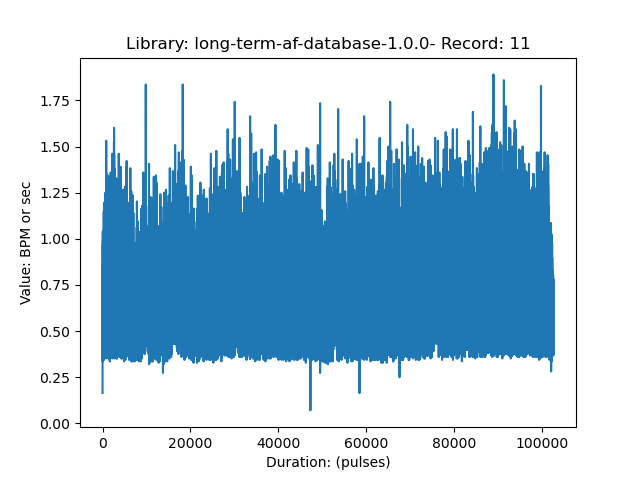
\includegraphics[width=.24\textwidth]{long-term-af-db/long-term-af-database-1.0.0_11.png}
		\caption{\gr Δείγμα βιβλιοθήκης \en Long Term AF Database \gr (αρχικά δείγματα/καταγραφές)}
	\end{figure}
	
	\item \en MIT-BIH Arrhythmia Database: \gr περιέχει 48 καταγραφές που ανήκουν σε 47 ασθενείς, με διάρκεια ελαφρώς μεγαλύτερη της μισής ώρας. Τα σήματα εδώ είναι συντομότερα και ο θόρυβος δε φαίνεται να πυκνώνει ακραία το σήμα. Συγκριτικά, λοιπόν, με την προηγούμενη βιβλιοθήκη παρατηρούνται με μεγαλύτερη ευυκολία περιοχές φυσιολογικής και μη λειτουργίας ακόμα και με το μάτι. Δε γίνεται συγκεκριμένος ο τύπος αρρυθμιών σε αυτή τη συλλογή, άρα γίνεται η υπόθεση πως περιέχει περισσότερες από μία. Η μορφολογία των σημάτων 
	διαφέρει: συμπεριλαμβάνονται τόσο σήματα με έντονο θόρυβο και μόνιμα άστατο καρδιακό ρυθμό, όσο και σήματα με ποικιλομορφίες (φαινομενική ομοιομορφία/ ηρεμία παλμών και ξαφνική απώλεια παλμών ή εμφάνιση πολύ υψηλών αριθμητικά τιμών). Είναι, επομένως, πιο εύκολα ερμηνεύσιμα σε σύγκριση με μερικές από τις υπόλοιπες μελετώμενες βιβλιοθήκες (Σχήμα 4.2). 
	\begin{figure}
		\centering
		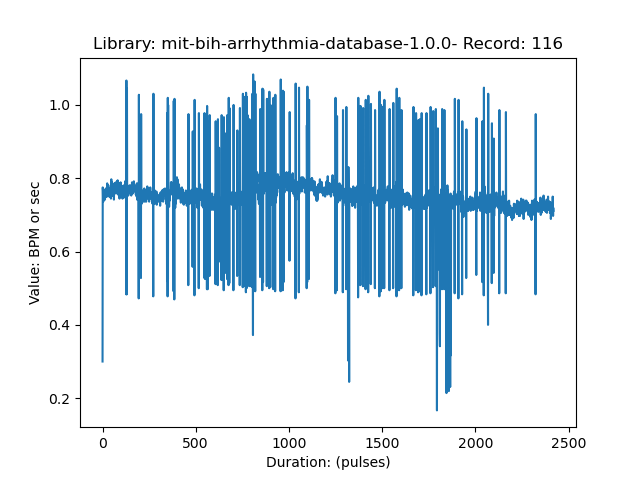
\includegraphics[width=.24\textwidth]{mitbih-arr-db/mit-bih-arrhythmia-database-1.0.0_116.png}
		\caption{\gr Δείγμα βιβλιοθήκης \en MIT-BIH Arrhythmia Database \gr (αρχικά δείγματα/καταγραφές)}
	\end{figure}
	\item \en MIT-BIH Atrial Fibrillation Database: \gr περιλαμβάνει 25 καταγραφές από ασθενείς με (κατά βάση) παροξυσμική κολπική μαρμαρυγή. Η διάρκεια των σημάτων είναι πολύ σύντομη, επομένως η εκτίμηση περιοχών μη φυσιολογικής λειτουργίας παρεμποδίζεται λόγω έλλειψης παρεμφερών δειγμάτων (Σχήμα 4.3).
	\begin{figure}
		\centering
		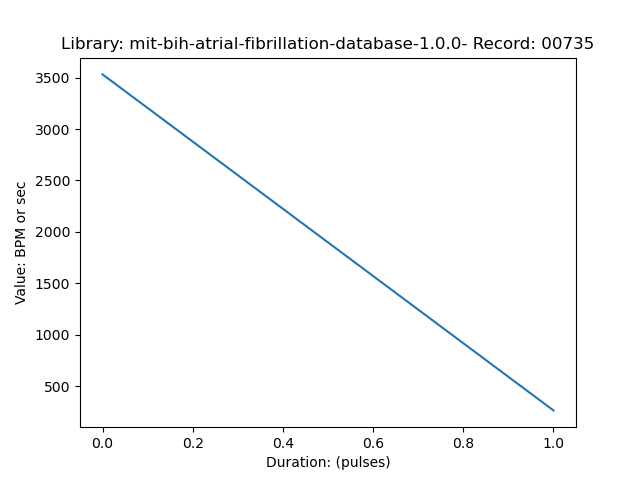
\includegraphics[width=.24\textwidth]{mitbih-af/mit-bih-atrial-fibrillation-database-1.0.0_00735.png}
		\caption{\gr Δείγμα βιβλιοθήκης \en MIT-BIH Atrial Fibrillation Database \gr (αρχικά δείγματα/καταγραφές)}
	\end{figure}
	\item \en MIT-BIH Malignant Ventricular Ectopy Database: \gr αυτή η ομάδα καταγραφών περιέχει κοιλιακές αρρυθμίες (παρατεταμένη κοιλιακή ταχυκαρδία, κοιλιακό πτερυγισμό και κοιλιακή μαρμαρυγή). Οι 22 καταγραφές έχουν διάρκεια μισής ώρας. Παρεμφερής με τη βιβλιοθήκη \en MIT-BIH Atrial Fibrillation Database \gr παρατηρείται η μικρής έκτασης διάρκεια στις καταγραφές και τίθεται το ερώτημα της δυνατότητας εξαγωγής συμπερασμάτων από αυτή τη συλλογή σημάτων (Σχήμα 4.4). 
	\begin{figure}
		\centering
		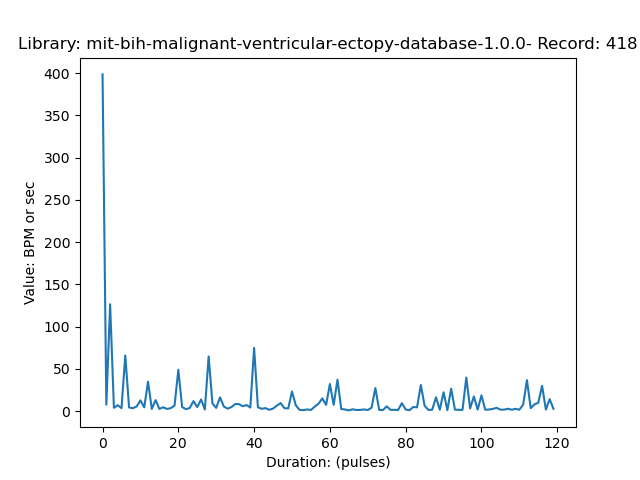
\includegraphics[width=.24\textwidth]{malignant/mit-bih-malignant-ventricular-ectopy-database-1.0.0_418.png}
		\caption{\gr Δείγμα βιβλιοθήκης \en MIT-BIH Malignant Ventricular Ectopy Database \gr (αρχικά δείγματα/καταγραφές)}
	\end{figure}
	\item \en MIT-BIH Supraventricular Arrhythmia Database: \gr αποτελείται από 78 καταγραφές διάρκειας 30 λεπτών (ανάμεσα σε 30 και 40) και οι ασθενείς υπέστησαν επεισόδια υπερκοιλιακών αρρυθμιών. Η τριαντάλεπτη καταγραφή κάνει πιο εύκολη τη διάκριση ανάμεσα σε αποκλίνοντες καρδιακούς παλμούς ακόμα και με το μάτι και διευκολύνει τόσο την ερμηνεία όσο και την αξιολόγηση των δειγμάτων. Όπως και στις υπόλοιπες βιβλιοθήκες, ο έντονος θόρυβος που παρατηρείται \en (spikes) \gr δεν είναι πραγματικοί καρδιακοί παλμοί αλλά θόρυβος που εμφανίζεται κατά την καταγραφή και δημιουργία των ηλεκτροκαρδιογραφημάτων (Σχήμα 4.5).
	\begin{figure}
		\centering
		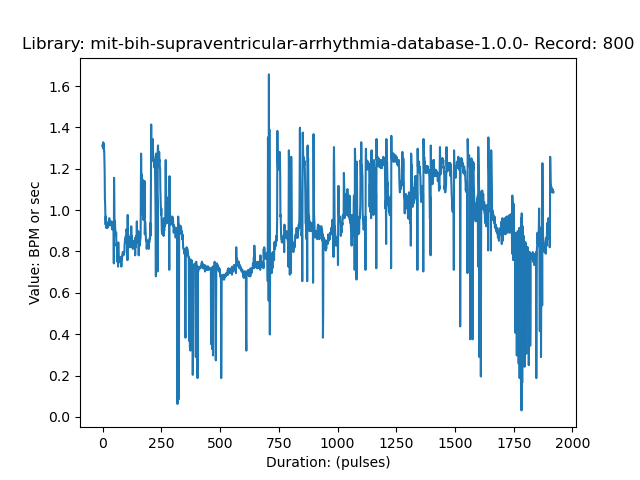
\includegraphics[width=.24\textwidth]{mitbih-supraventricular-db/mit-bih-supraventricular-arrhythmia-database-1.0.0_800.png}
		\caption{\gr Δείγμα βιβλιοθήκης \en MIT-BIH Supraventricular Arrhythmia Database \gr (αρχικά δείγματα/καταγραφές)}
	\end{figure}
	\item \en CU Ventricular Tachyarrhythmia Database: \gr αποτελείται από 35 καταγραφές διάρκειας περίπου 8 λεπτών και οι ασθενείς υπέστησαν επεισόδια παρατεταμένης κοιλιακής ταχυκαρδίας, κοιλιακού πτερυγισμού και κοιλιακής μαρμαρυγής. Από τα αρχικά ανεπεξέργαστα δείγματα παρατηρείται μεμονωμένος θόρυβος, δε φαίνεται, δηλαδή, να εμφανίζεται σε συνεχόμενα διαστήματα· γεγονός ενθαρρυντικό καθώς ο θόρυβος φαίνεται να είναι μειωμένος σε αντίθεση με άλλες συλλογές δεδομένων, διευκολύνοντας την εξαγωγή συμπερασμάτων. (Σχήμα 4.6)
	\begin{figure}
		\centering
		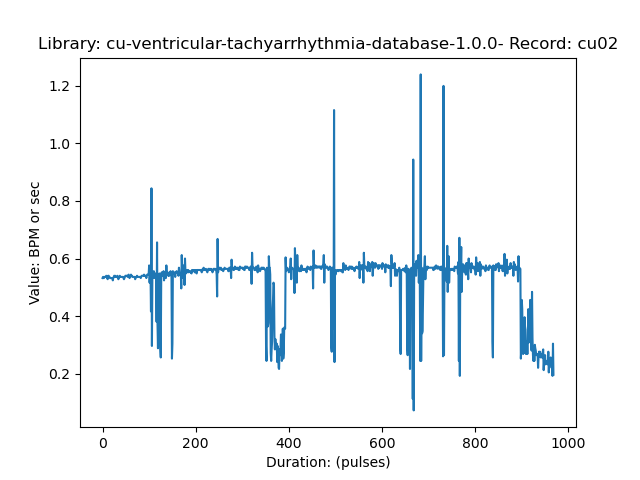
\includegraphics[width=.24\textwidth]{cu-ventricular/cu-ventricular-tachyarrhythmia-database-1.0.0_cu02.png}
		\caption{\gr Δείγμα βιβλιοθήκης \en CU Ventricular Tachyarrhythmia Database \gr (αρχικά δείγματα/καταγραφές)}
	\end{figure}
	\item \en Congestive Heart Failure RR Interval Database: \gr περιέχει 29 καταγραφές και η διάρκεια ποικίλει ανάλογα με την καταγραφή (Σχήμα 4.7).  Οι καταγραφές φαίνεται να περιέχουν μικρότερο ποσοστό θορύβου, γεγονός που αφήνει το σήμα σχετικά ανεπηρέαστο μετά την αφαίρεσή του.\gr
	\begin{figure}
		\centering
		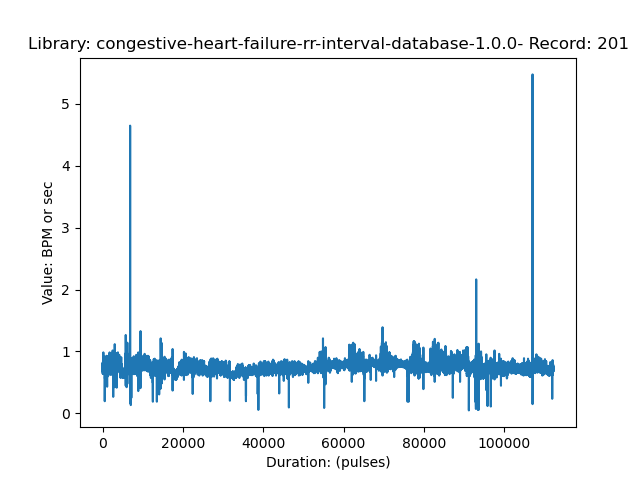
\includegraphics[width=.24\textwidth]{congestive-hf-db/congestive-heart-failure-rr-interval-database-1.0.0_201.png}
		\caption{ \gr Δείγμα βιβλιοθήκης \en Congestive Heart Failure RR Interval Database \gr (αρχικά δείγματα/καταγραφές)}
	\end{figure}
	\item \en CTU-CHB Intrapartum Cardiotocography Database: \gr περιέχει 552 δείγματα από εγκυμονούσες ασθενείς. Οι καταγραφές αποτελούν καρδιοτοκογραφήματα, τα οποία μπορούν να υποστούν επεξεργασία όμοια με τα ηλεκτροκαρδιογραφήματα. Οι καταγραφές έχουν διάρκεια μέχρι και 90 λεπτά (Σχήμα 4.8) πριν τη διαδικασία του ενεργού τοκετού. Η βιβλιοθήκη περιέχει επιπλέον αξιολόγηση διαφορετικών βιοχημικών παραγόντων όπως ο χρόνος κύησης, η πιθανότητα καισαρικής τομής, δεδομένα αναφορικά στη μητέρα και τα φυλετικά χαρακτηριστικά του μωρού. Τα σήματα αποτελούν από τα πιο έντονα σε μορφολογία, λόγω της ιδιαιτερότητας της φυσικής κατάστασης των ασθενών (γυναίκες κατά τη διάρκεια τοκετού, συσπάσεων).
	\begin{figure}
		\centering
		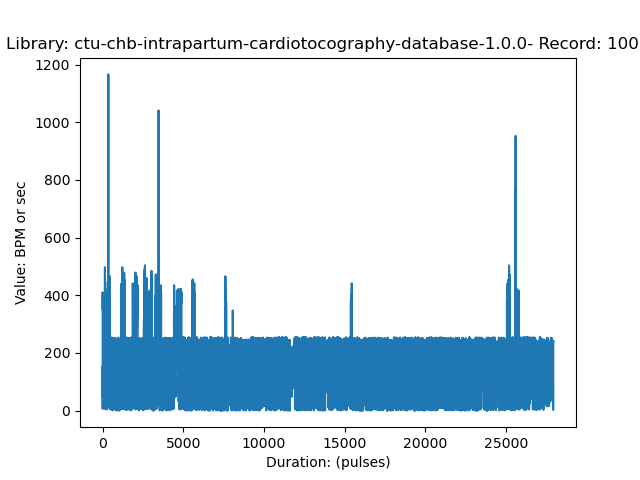
\includegraphics[width=.24\textwidth]{ctu/ctu-chb-intrapartum-cardiotocography-database-1.0.0_1001.png}
		\caption{Δείγμα βιβλιοθήκης \en CTU-CHB Intrapartum Cardiotocography Database \gr (αρχικά δείγματα/καταγραφές)}
	\end{figure}
	\item Fantasia Database: \gr 40 καταγραφές από είκοσι άτομα νεαρής ηλικίας και είκοσι ηλικιωμένους διάρκειας (ίση αναλογία γυναικών και ανδρών) 120 λεπτών. Η καταγραφή πραγματοποιήθηκε ενώ οι εθελοντές βρίσκονται σε κατάσταση ανάπαυσης και παρακολουθούν την ταινία \en Fantasia. \gr Αυτή η βάση δεδομένων αποτελείται από καταγραφές φυσιολογικής καρδιακής λειτουργίας σε κατάσταση ηρεμίας (υγιή άτομα, χωρίς καρδιακές παθήσεις) και συμπεριλήφθηκε για μια πιο ολοκληρωμένη εφαρμογή του αλγορίθμου (Σχήμα 4.9). Όπως παρατηρείται από το αρχικό δείγμα καταγραφών, υπάρχει θόρυβος ο οποίος διαχωρίζεται ευκολότερα μιας και η γεικότερη εικόνα των παλμών είναι ομοιόμορφη, χωρίς εμφάνιση αρρυθμιών.
	\begin{figure}
		\centering
		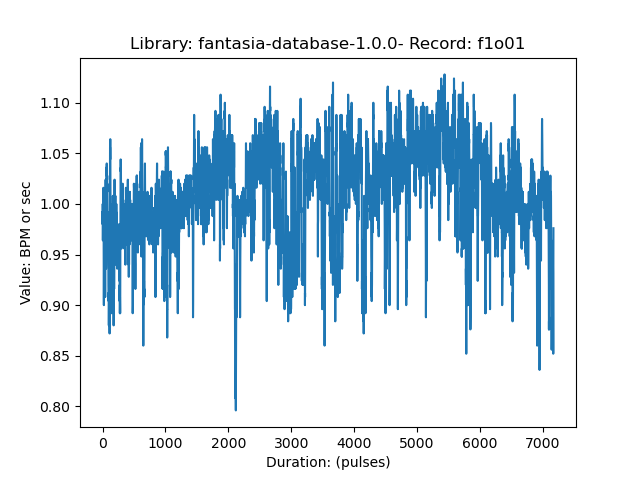
\includegraphics[width=.24\textwidth]{Fantasia/fantasia-database-1.0.0_f1o01.png}
		\caption{\gr Δείγμα βιβλιοθήκης \en Fantasia Database \gr (αρχικά δείγματα/καταγραφές)}
	\end{figure}
	\item Normal Sinus Rhythm RR Interval Database: \gr αποτελείται από 54 καταγραφές (η διάρκεια δεν είναι συγκεκριμένη) από 30 άνδρες ηλικίας 28 έως 76 ετών και 24 γυναίκες ηλικίας 58 έως 73 ετών (Σχήμα 4.10). Τα σήματα καταγράφηκαν σε κατάσταση ηρεμίας (δεν προσδιορίζεται αν οι εθελοντές πάσχουν από κάποια καρδιακή πάθηση) και η διάρκειά τους είναι μεγαλύτερη από 2 ώρες. Η παρουσία έντονων κορυφών παρατηρείται και σε αυτό το σύνολο καταγραφών· δεν αποτελούν, όμως, αρρυθμίες παρά το θόρυβο που αποτυπώθηκε κατά τη διάρκεια της καταγραφής (και αφαιρείται στη συνέχεια), έτσι ώστε να είναι εγκυρότερη η μελέτη, επεξεργασία και αξιολόγηση των σημάτων. 
	\begin{figure}
		\centering
		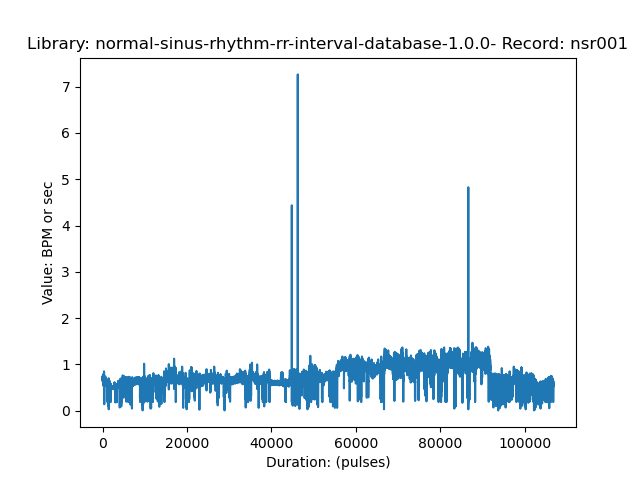
\includegraphics[width=.24\textwidth]{nsr/normal-sinus-rhythm-rr-interval-database-1.0.0_nsr001.png}
		\caption{\gr Δείγμα βιβλιοθήκης \en Normal Sinus Rhythm RR Interval Database \gr (αρχικά δείγματα/καταγραφές)}
	\end{figure}
\end{itemize}
\gr
\par
Παρατηρείται πως τα αρχικά σήματα δεν είναι κατάλληλα προς επεξεργασία στην αρχική τους μορφή. Οι συνθήκες καταγραφής έχουν εισάγει θόρυβο λόγω κακής επαφής των ηλεκτροδίων, κίνησης του ασθενούς ή αποκλίσεις του μηχανήματος. Γίνεται, λοιπόν, αναγκαία μια προεπεξεργασία προκειμένου να "φιλτραριστούν" τα σήματα. Μετά το φιλτράρισμα αυτό, τα σήματα θα είναι ευκολότερο να μελετηθούν, να επεξεργαστούν και να εφαρμοστούν οι αναγκαίες μέθοδοι και να εξαχθούν αποτελέσματα. 
\par
Τα αποτελέσματα αξιολογήθηκαν με βάση τη μορφολογία του σήματος (διάρκεια των καταγραφών, πυκνότητα αρρυθμιών ή/και έκτοπων συστολών). Η διάρκεια των σημάτων και τα διαφορετικά χαρακτηριστικά της κάθε βιβλιοθήκης παρουσιάζονται ξεχωριστά για την καθεμία.

\subsection{Μορφοποίηση πειραμάτων και κώδικας}
Για τη διεξαγωγή αυτών των πειραμάτων δομήθηκε ένας αλγόριθμος, του οποίου ο σκελετός είναι όμοιος με αυτόν που δημιουργήθηκε για το Έργο 82475/110444 - \en HOMore, \gr μιας και τα πειράματα του έργου αποτελούν μέρος αυτής της εργασίας. Η διαδικασία αποσκοπούσε στην απομάκρυνση του θορύβου από κάθε σήμα, όσο αυτό είναι εφικτό, και στη συνέχεια η μελέτη και επεξεργασία των σημάτων μέσω των παραθύρων. Τα παράθυρα δεν είναι τίποτα άλλο παρά τμήματα του ολικού σήματος χωρισμένα σε συγκεκριμένα χρονικά διαστήματα τα οποία καθορίστηκαν τυπικά, ως άξονας σύγκρισης ανάμεσα στις διαφορετικές βιβλιοθήκες (τα μεγέθη τους κυμαίνονται από 15 δευτερόλεπτα έως και 5 λεπτά). Σε κάθε ξεχωριστό παράθυρο, υπολογίζονται οι μετρικές και οι μέθοδοι εκτίμησης εντροπίας και στο τέλος αποτυπώνονται στο γράφημα τα τμήματα/παράθυρα με τις υψηλότερες τιμές της εκάστοτε εξεταζόμενης μετρικής που έφεραν τα υψηλότερα αποτελέσματα. Οι υψηλότερες τιμές αντιστοιχούν σε υψηλό και ακανόνιστο καρδιακό παλμό, δηλαδή αποτελούν τις περιοχές στις οποίες πρέπει να εστιαστεί η προσοχή του μελετητή (ως οι πιο επικίνδυνες).
\subsection{Τα βήματα}
Πιο συγκεκριμένα, τα βήματα του αλγορίθμου είναι τα ακόλουθα:
Σε πρώτο στάδιο, τα σήματα υπέστησαν προεπεξεργασία. Πραγματοποιήθηκε υπολογισμός των διαστημάτων \en RR \gr με βάση τα αρχικά δεδομένα καθώς αυτά δε βρίσκονταν στην επιθυμητή μορφή. Τα δεδομένα τροποποιούνται έτσι ώστε να μπορούν να υποστούν επεξεργασία σε όλες τις βιβλιοθήκες με τον ίδιο τρόπο. Αυτό πραγματοποιείται υπολογίζονταις τις αριθμητικές διαφορές ανάμεσα στους συνεχόμενους παλμούς. Οι βιβλιοθήκες που χρησιμοποιήθηκαν μετρώνται σε δευτερόλεπτα ή σε χτύπους ανά λεπτό. Ως τελικό βήμα καθορίζεται η αφαίρεση του θορύβου για την καλύτερη δυνατή εκτίμηση.
\par
Σε δεύτερο στάδιο, καθορίζονται οι τιμές των παραμέτρων. Η πρώτη παράμετρος είναι το μέγεθος του παραθύρου στο οποίο θα υπολογιστούν οι μέθοδοι και οι μέθοδοι εκτίμησης εντροπίας του \en HRV. \gr Οι δυνατές τιμές που μπορεί να λάβει αυτή η παράμετρος είναι 15, 30, 60, 120, 180, 240 και 300 (αντιστοιχούν σε δευτερόλεπτα). Στις βιβλιοθήκες με πιο σύντομες καταγραφές, το μέγεθος του παραθύρου κυμάνθηκε από 15 σε 60 δευτερόλεπτα. Στη συνέχεια αφαιρέθηκε ο θόρυβος. Ως πρώτο βήμα, απομακρύνθηκαν από το σήμα οι μηδενικές τιμές. Σε μερικές περιπτώσεις η τιμή μηδέν αντιστοιχεί σε απουσία παλμού, ενώ σε άλλες χειροκίνητη αφαίρεση θορύβου από το σήμα, ακόμα και απουσία καταγραφής λόγω κίνησης των ηλεκτροδίων. Αφαιρέθηκαν, επομένως, από το σήμα σε μια προσπάθεια αποφυγής αλλοίωσης των αποτελεσμάτων. Το δεύτερο φίλτρο που χρησιμοποιήθηκε "κόβει" τις ακραίες αριθμητικές τιμές όταν αυτές διαφέρουν περισσότερο από 25 τοις εκατό από τη μέση τιμή του σήματος (δοκιμάστηκαν διαφορετικά κατώφλια ώστε να επιλεχθεί η συγκεκριμένη ως καταλληλότερη). Το τρίτο φίλτρο που χρησιμοποιήθηκε συλλέγει όλες οι κορυφές του σήματος που απέχει αλγεβρικά (τιμή είτε υψηλότερη είτε χαμηλότερη) τουλάχιστον 25\% από τη διάμεσο των τριών προηγούμενων \en RR \gr διαστημάτων. Σε αυτές τις κορυφές έγινε αντικατάσταση της τιμής με τη διάμεσο. Το τέταρτο και τελευταίο φίλτρο είναι αρκετά απλό, καθώς θεωρεί ως θόρυβο τους παλμούς που απέχουν αριθμητικά από τον επόμενό τους περισσότερο από 25 τοις εκατό. Η τιμή αυτών των παλμών αντικαθίσταται σε αυτή την περίπτωση από την τιμή του επόμενου παλμού.
\par
Το τελικό βήμα ήταν η εκτίμηση των μετρικών, των μεθόδων εκτίμησης εντροπίας και των κυματιδίων \en Haar \gr σε κάθε ένα από τα δημιουργούμενα παράθυρα. Οι σκάλες εκτίμησης των κυματιδίων \en Haar \gr κυμαίνοται από δύο έως δέκα, έτσι ώστε να καλυφθεί μεγαλύτερο εύρος τιμών για πιο ακριβείς μετρήσεις (ως μέγιστη τιμή επιλέχθηκε το δέκα, μιας και σε υψηλότερες κλίμακες υπήρξε σύγκλιση των αποτελεσμάτων).
\par
Υπολογίστηκαν επίσης οι μέσες τιμές των μετρικών και μεθόδων για ολόκληρο το σήμα· οι τιμές, δηλαδή, που προέκυψαν από κάθε παράθυρο προστιθέμενες και διαιρεμένες με το μήκος των μετρήσεων του κύματος. Τα γραφήματα δημιουργήθηκαν από τις εκτιμώμενες τιμές του κάθε παραθύρου (κάθε "δείγμα" αποτελεί την τιμή του σήματος ή της εκάστοτε μετρικής και μεθόδου σε ένα συγκεκριμένο παράθυρο). Για τα αποτελέσματα του αλγορίθμου χρησιμοποιήθηκαν όλες οι μετρικές και μέθοδοι και σε κάθε βιβλιοθήκη εντοπίστηκαν οι πιο ακριβείς. Το πόρισμα αυτό προκύπτει από τα πειράματα τα οποία πραγματοποιήθηκαν σε αυτή τη διπλωματική εργασία, έπειτα από παρατήρηση των αποτελεσμάτων. 
\par
Με αυτό το σκεπτικό, επιλέχθηκαν οι υψηλότερες τιμές του πειράματος από την κάθε μία (από την πρώτη έως και τις έξι υψηλότερες) ώστε να προβληθούν στο τελικό διάγραμμα (το πλήθος των επιλεγμένων τιμών μεταβάλλεται εύκολα διότι αποτελεί παράμετρο της εκτέλεσης των πειραμάτων στο τερματικό). Ακόμα, μαζί με αυτές τις μετρικές, στη γραφική παράσταση του κάθε καρδιογραφήματος υπολογίζονται και οι τέσσερις υψηλότερες (σε τιμή) εκτιμήσεις των κυματιδίων \en Haar. \gr  
\par
Συνοπτικά, παραθέτονται τα βήματα του αλγορίθμου για τον εντοπισμό επικίνδυνων περιοχών κατά τη διάρκεια εξαγωγής των πειραμάτων.
\begin{itemize}
	\item Φιλτράρισμα των σημάτων.
	\item Προσδιορισμός των παραθύρων που θα χρησιμοποιηθούν. 
	\item Για κάθε ξεχωριστό παράθυρο, υπολογισμός των μετρικών.
	\item Για κάθε ξεχωριστό παράθυρο, υπολογισμός των μεθόδων εκτίμησης εντροπίας.
	\item Επιλογή των παραθύρων με τις υψηλότερες τιμές μετρικών ή μεθόδων.  
	\item Υπολογισμός των συντεταγμένων των συγκεκριμένων παραθύρων (τα παράθυρα είναι ισομεγέθη, στις περισσότερες περιπτώσεις 60 δευτερόλεπτα).
	\item Υπολογισμός γραφήματος (οι επικίνδυνες περιοχές διαφοροποιούνται για να είναι ευκολότερη η εστίαση του μελετητή ή του ιατρικού ερευνητή/γιατρού). Συνολικά για κάθε σήμα παράγονται γραφήματα με τις εκτιμώμενες επικίνδυνες περιοχές τόσο των μετρικών όσο και των κυματιδίων \en Haar. \gr Η διαδικασία αυτή επαναλαμβάνεται για όλα τα δείγματα κάθε βιβλιοθήκης. 
\end{itemize}


\subsection{Καθορισμός παραμέτρων}
Οι αναγκαίες παράμετροι στη διεκπεραίωση των ερευνητικών πειραμάτων ήταν οι ακόλουθες:
\begin{itemize}
	\item το μέγεθος του παραθύρου επεξεργασίας που λαμβάνει την τιμή του χρονικού διαστήματος σε δευτερόλεπτα (όνομα παραμέτρου στον κώδικα: $window size$)
	\item στη μέθοδο αφαίρεσης θορύβου, ο συνυπολογισμός των τριών προηγούμενων δειγμάτων από τα οποία υπολογίζεται το ποσοστό διαφοράς από τη διάμεσο (όνομα παραμέτρου στον κώδικα: $n previous values$) 
	\item το κατώφλι που επιλέχθηκε σε κάθε φίλτρο αφαίρεσης θορύβου (όνομα παραμέτρου στον κώδικα: $threshold$)
	\item η σκάλα ή επίπεδο στον υπολογισμό των κυματιδίων \en Haar \gr (όνομα παραμέτρου στον κώδικα: $scale$)
	\item η παράμετρος διάστασης του \en m-\gr διάστατου χώρου στον οποίο ενσωματώνεται το σήμα στις μεθόδους \en Approximate Entropy, Sample Entropy, Bubble Entropy \gr (όνομα παραμέτρου στον κώδικα: $m$)
	\item η παράμετρος κλίμακας (φίλτρο θορύβου) στις μεθόδους \en Approximate Entropy, Sample Entropy, Bubble Entropy \gr (όνομα παραμέτρου στον κώδικα: $r$)
\end{itemize}

\par
Συνοπτικά, η πορεία επεξεργασίας των σημάτων και ο αλγόριθμος παρουσιάζονται στο ακόλουθο διάγραμμα (Σχήμα 4.11):
\begin{figure}
	\centering
	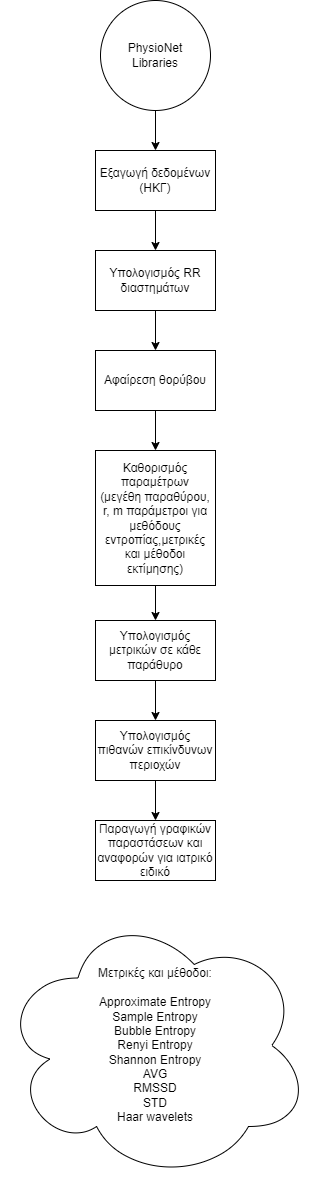
\includegraphics[width=0.4\textwidth]{Algorithm.png}
	\caption{Διαγραμματική απεικόνιση του αλορίθμου επεξεργασίας καρδιακών σημάτων}
\end{figure}


\section{Αποτελέσματα πειραματικής ανάλυσης}
Ο σχολιασμός κάθε βιβλιοθήκης θα παρατεθεί στη συνέχεια εξ ολοκλήρου για την κάθε μία, από την παραγωγή των διαγραμμάτων έως και το σχολιασμό των αποτελεσμάτων. 
\par 
\textbf{Σημείωση:} Στη συνέχεια παρουσιάζεται αυξημένο πλήθος πειραμάτων και κατά συνέπεια διαγραμμάτων, κάτι που μπορεί να κουράσει τον αναγνώστη. Ο όγκος αυτός δεν ήταν δυνατό να περιοριστεί διότι αποτελεί απόδειξη της λειτουργίας και απόδοσης του αλγορίθμου. Για αυτό το σκοπό, στο τέλος του κεφαλαίου πραγματοποιείται μια πιο συνοπτική ανακεφαλαίωση, ώστε να γίνει ευκολότερη η ερμηνεία των αποτελεσμάτων.
\par
\subsection{\en Long Term AF Database \gr}
Σε αυτή τη βιβλιοθήκη τα μεγέθη των παραθύρων που εφαρμόστηκαν (σε δευτερόλεπτα) ήταν τα [60, 120, 240, 300]. Τα δείγματα αυτής της βιβλιοθήκης αποτελούν αρνητικά παραδείγματα, διότι η διάρκεια των σημάτων είναι εκτενής. Αυτό, όμως που καθιστά τις εκτιμήσεις δύσκολες και πιθανώς άστοχες είναι η ένταση των παλμών στις καταγραφές. Τα σήματα είναι δασώδη, ή πριονωτά, κάτι που καθιστά το σήμα δύσκολο να ερμηνευθεί. Λίγες είναι οι περιπτώσεις στις οποίες τα δείγματα ευνοούν τις προβλέψεις και εκτιμήσεις του αλγορίθμου. 
Τα σήματα αρχικά είχαν την εξής εικόνα (χωρίς φιλτράρισμα θορύβου) (Σχήμα 4,12): 
\begin{figure}
	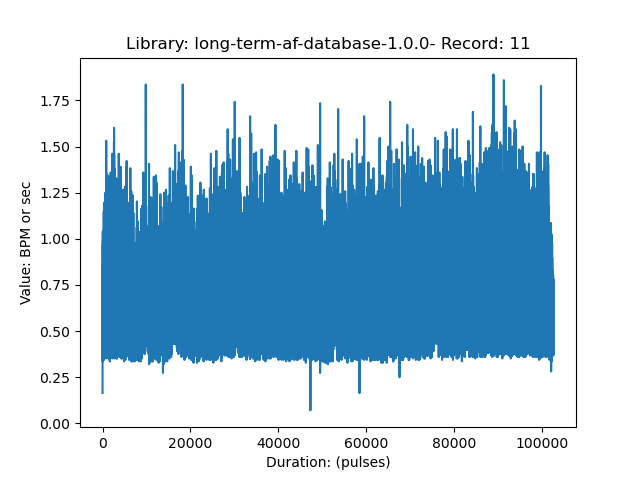
\includegraphics[width=.24\textwidth]{long-term-af-db/long-term-af-database-1.0.0_11.png}\hfill
	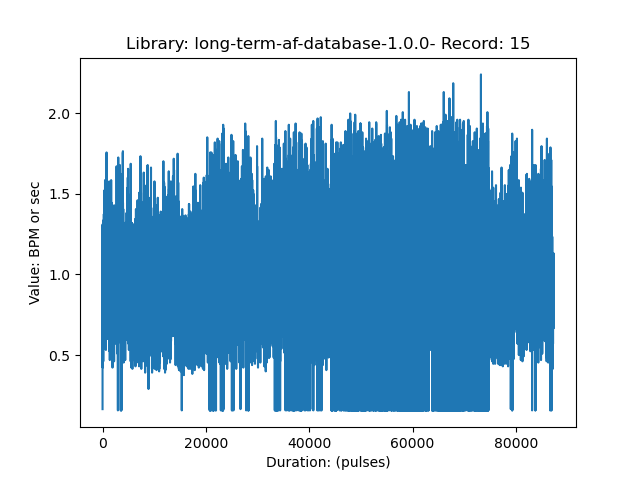
\includegraphics[width=.24\textwidth]{long-term-af-db/long-term-af-database-1.0.0_15.png}\hfill
	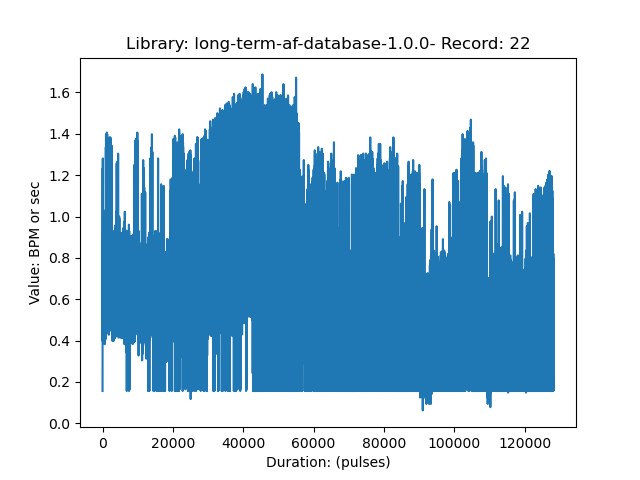
\includegraphics[width=.24\textwidth]{long-term-af-db/long-term-af-database-1.0.0_22.png}\hfill
	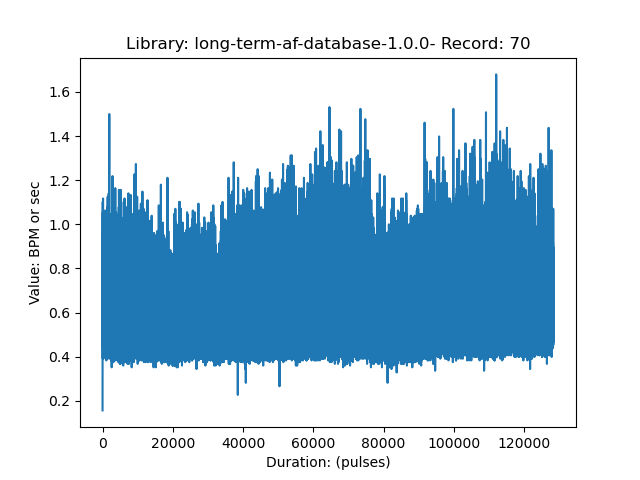
\includegraphics[width=.24\textwidth]{long-term-af-db/long-term-af-database-1.0.0_70.png}\hfill
	\\[\smallskipamount]
	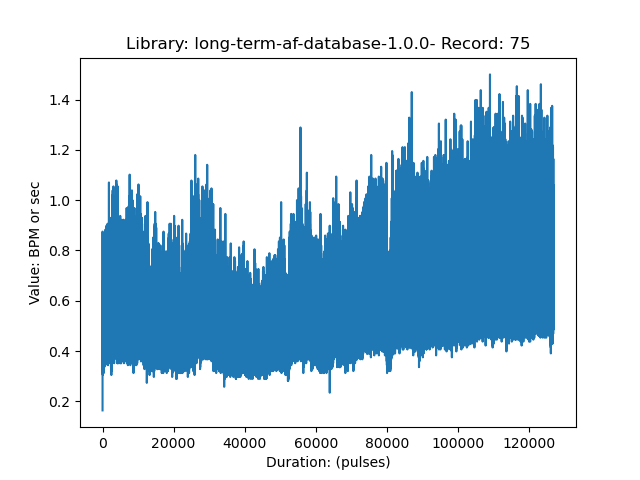
\includegraphics[width=.24\textwidth]{long-term-af-db/long-term-af-database-1.0.0_75.png}\hfill
	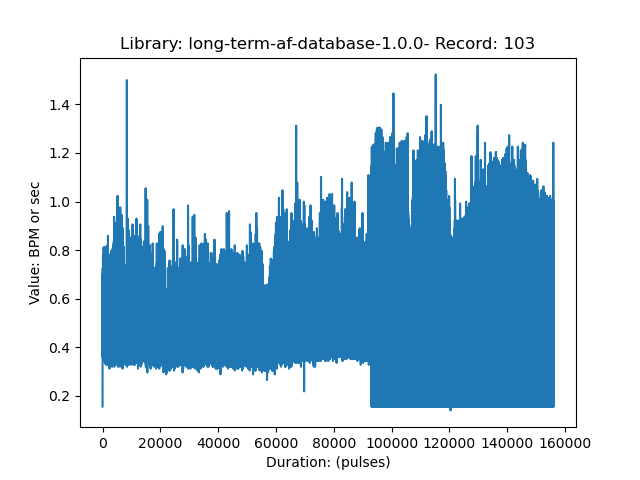
\includegraphics[width=.24\textwidth]{long-term-af-db/long-term-af-database-1.0.0_103.png}\hfill
	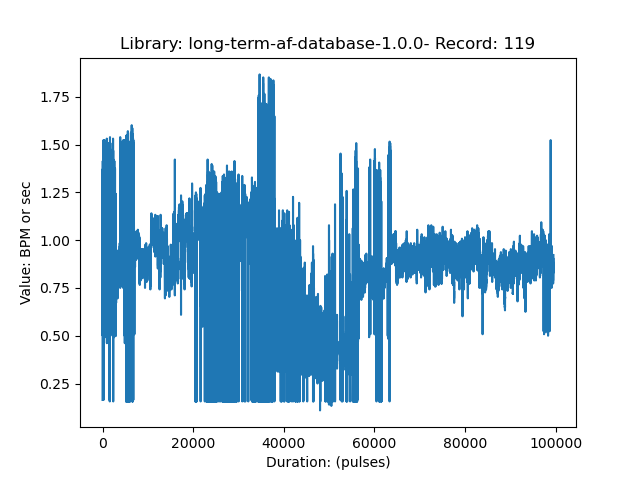
\includegraphics[width=.24\textwidth]{long-term-af-db/long-term-af-database-1.0.0_119.png}\hfill
	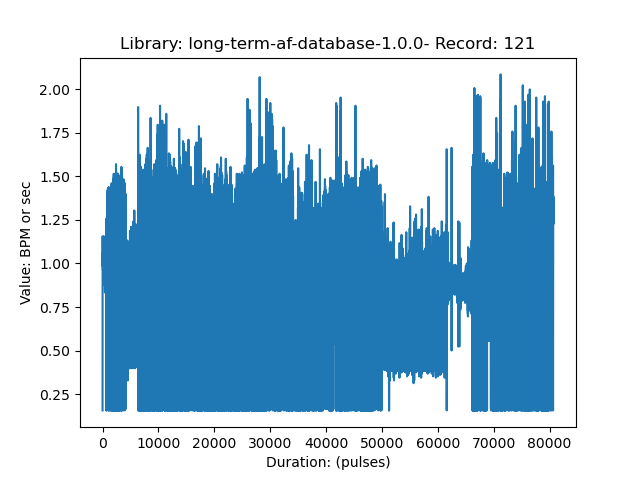
\includegraphics[width=.24\textwidth]{long-term-af-db/long-term-af-database-1.0.0_121.png}\hfill
	\\[\smallskipamount]
	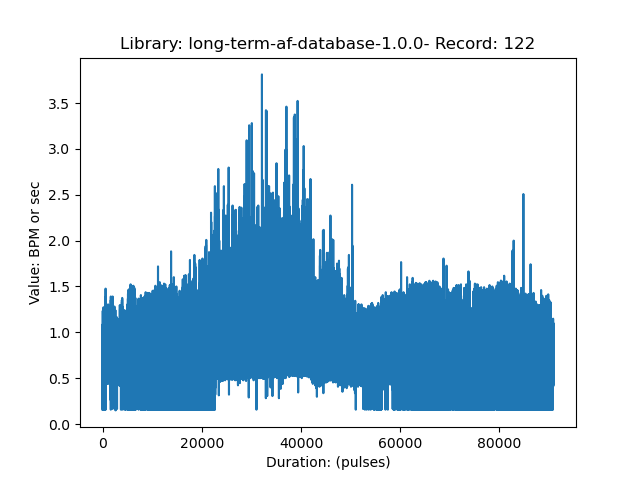
\includegraphics[width=.24\textwidth]{long-term-af-db/long-term-af-database-1.0.0_122.png}\hfill
	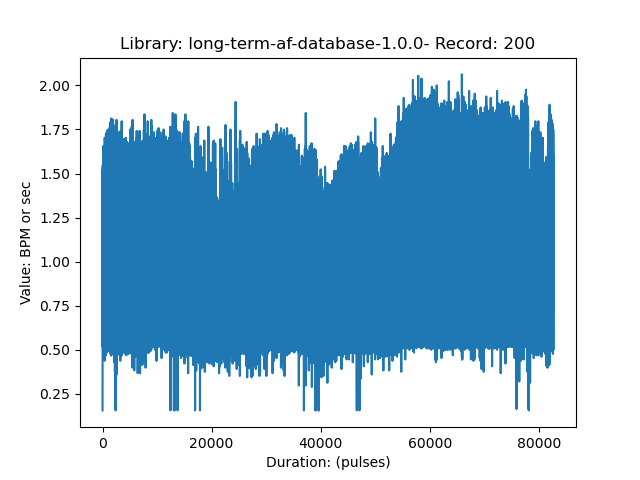
\includegraphics[width=.24\textwidth]{long-term-af-db/long-term-af-database-1.0.0_200.png}\hfill
	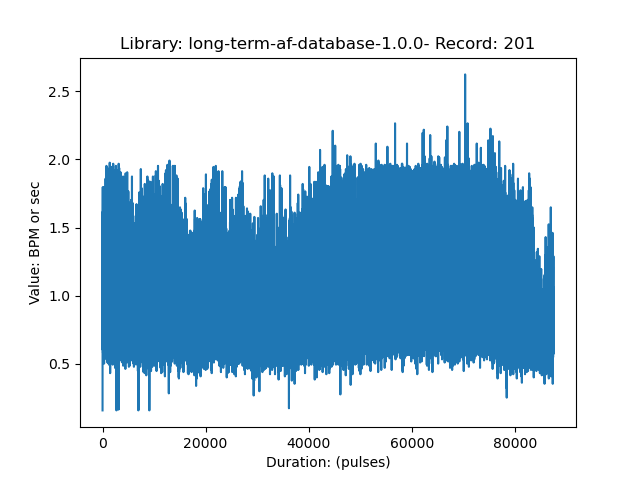
\includegraphics[width=.24\textwidth]{long-term-af-db/long-term-af-database-1.0.0_201.png}\hfill
	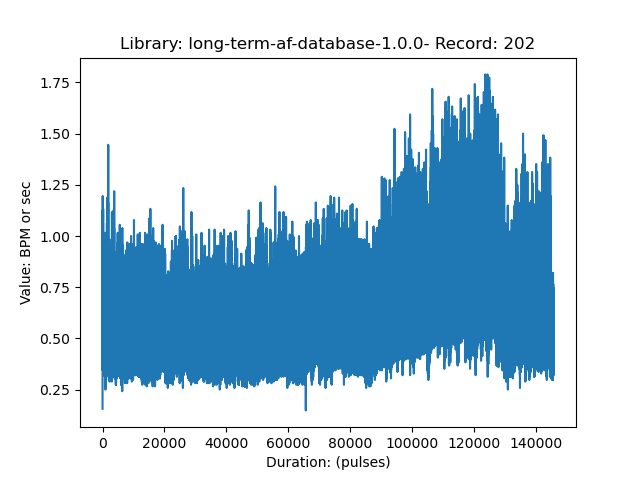
\includegraphics[width=.24\textwidth]{long-term-af-db/long-term-af-database-1.0.0_202.png}\hfill
	\caption{Συλλογή αποτελεσμάτων από τη βιβλιοθήκη \en Long Term AF Database \gr (αρχικά δείγματα/καταγραφές)}
\end{figure}
Μετά την εφαρμογή του αλγορίθμου τα αποτελέσματα ήταν τα εξής:
\begin{itemize}
	\item \en ApEn: \gr
	Τα αποτελέσματα αυτής της μεθόδου εκτίμησης εντροπίας δεν είναι εύστοχες. Κανένα από τα μεγέθη των παραθύρων δεν βελτιώνει ιδιαίτερα τις προβλέψεις. Ένα επιπλέον αρνητικό αποτέλεσμα αυτής της μεθόδου είναι πως όσο τα μεγέθη των παραθύρων μεταβάλλονται οι εκτιμήσεις της μεθόδου δεν παραμένουν σταθερές. Αυτό σημαίνει πως όσο τα παράθυρα αλλάζουν, η μέθοδος δε συνεχίζει να εστιάζει στην ίδια περιοχή, είτε η περιοχή είναι πιθανώς επικίνδυνη είτε όχι. 
	\par
	Μερικά ενδεικτικά δείγματα παρουσιάζονται στα Σχήματα 4.13 (παράδειγμα που υποδεικνύει την αλλαγή των "επικίνδυνων περιοχών" όσο τα παράθυρα αλλάζουν) και 4.14 (ενδεικτικά αποτελέσματα των εκτιμήσεων της \en ApEn) \gr: 
	\begin{figure}
		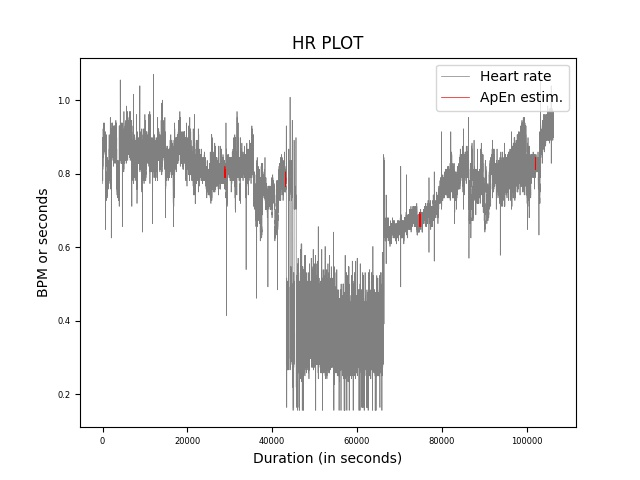
\includegraphics[width=.24\textwidth]{ApEn-long-term-af-db/long-term-af-database-1.0.0_00_60sec.jpeg}\hfill
		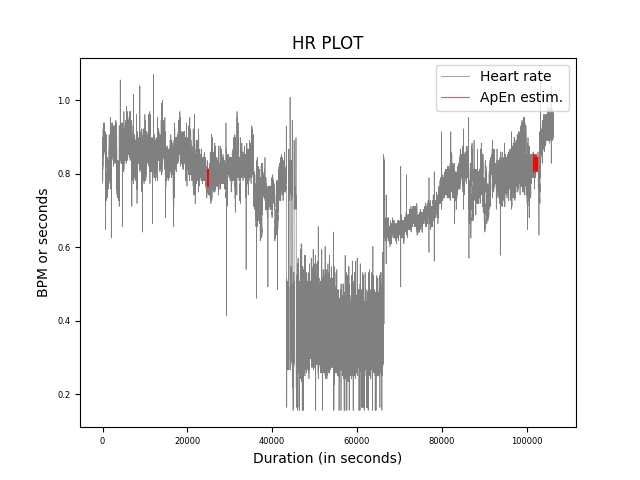
\includegraphics[width=.24\textwidth]{ApEn-long-term-af-db/long-term-af-database-1.0.0_00_120sec.jpeg}\hfill
		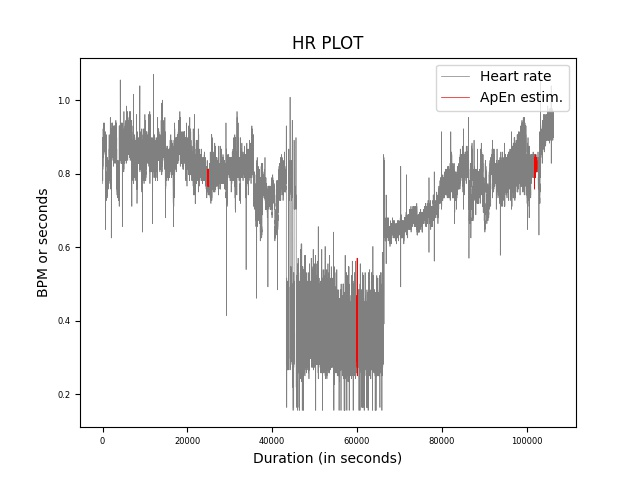
\includegraphics[width=.24\textwidth]{ApEn-long-term-af-db/long-term-af-database-1.0.0_00_180sec.jpeg}\hfill
		\centering
		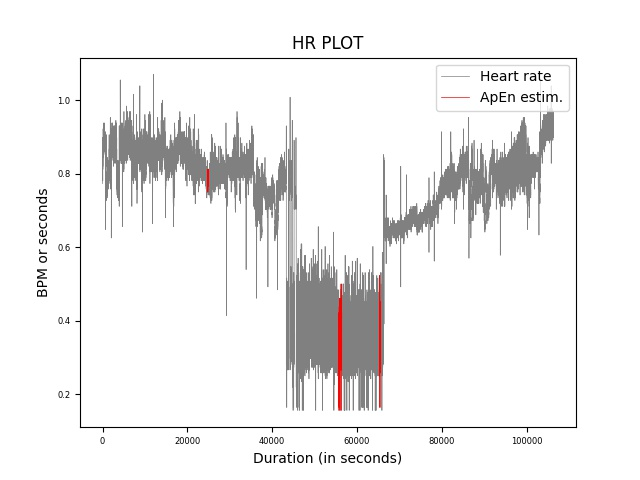
\includegraphics[width=.24\textwidth]{ApEn-long-term-af-db/long-term-af-database-1.0.0_00_240sec.jpeg}\hfill
		\caption{Συλλογή αποτελεσμάτων από τη βιβλιοθήκη \en Long Term AF Database \gr για τη μετρική \en ApEn \gr (αλλαγή μεγέθους παραθύρων)}
	\end{figure}
	\begin{figure}
		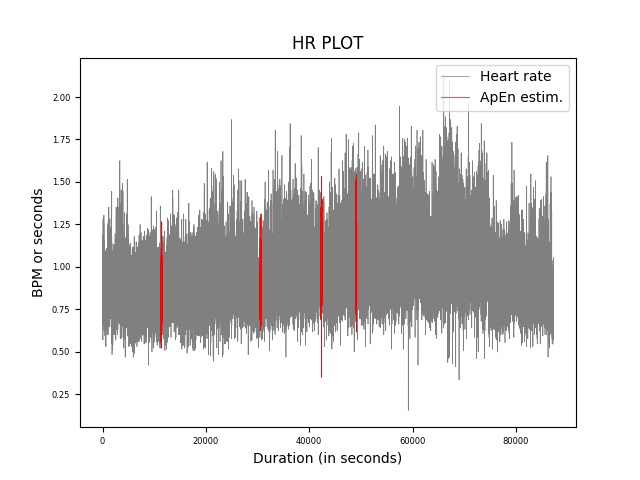
\includegraphics[width=.24\textwidth]{ApEn-long-term-af-db/long-term-af-database-1.0.0_15_240sec.jpeg}\hfill
		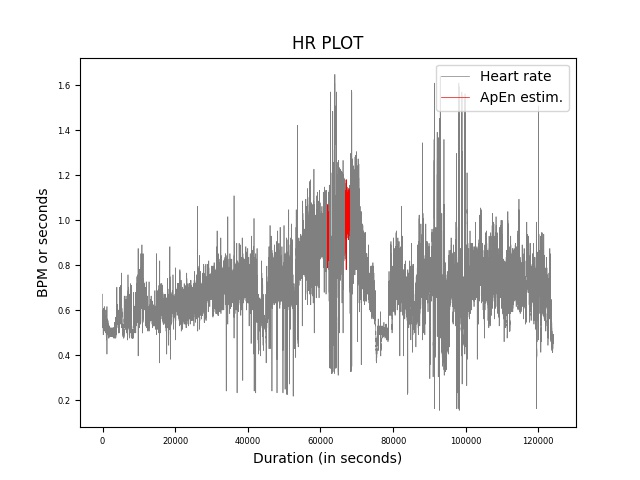
\includegraphics[width=.24\textwidth]{ApEn-long-term-af-db/long-term-af-database-1.0.0_16_240sec.jpeg}\hfill
		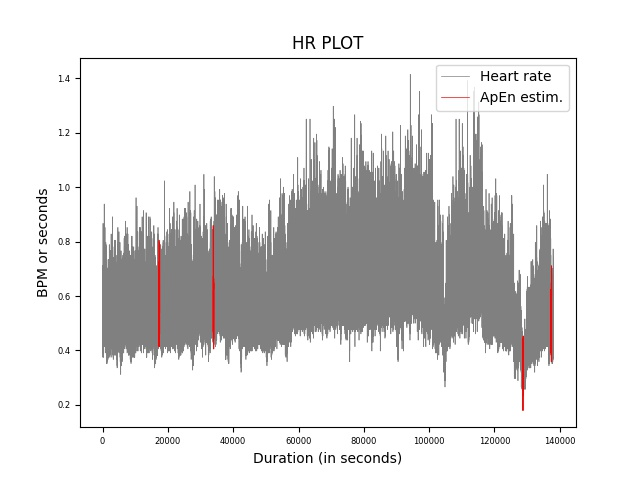
\includegraphics[width=.24\textwidth]{ApEn-long-term-af-db/long-term-af-database-1.0.0_17_240sec.jpeg}\hfill
		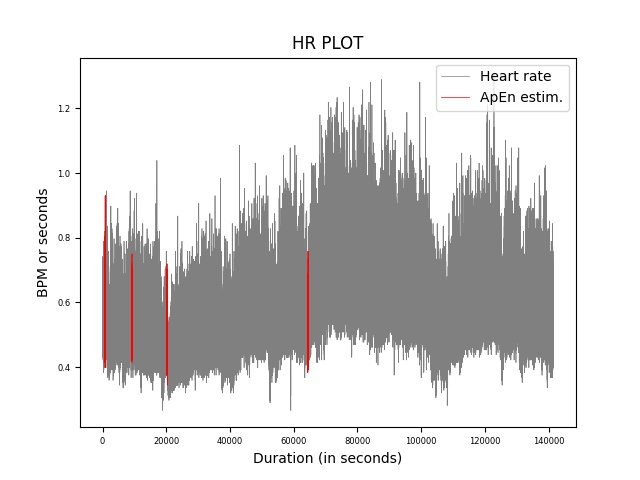
\includegraphics[width=.24\textwidth]{ApEn-long-term-af-db/long-term-af-database-1.0.0_18_240sec.jpeg}\hfill
		\\[\smallskipamount]
		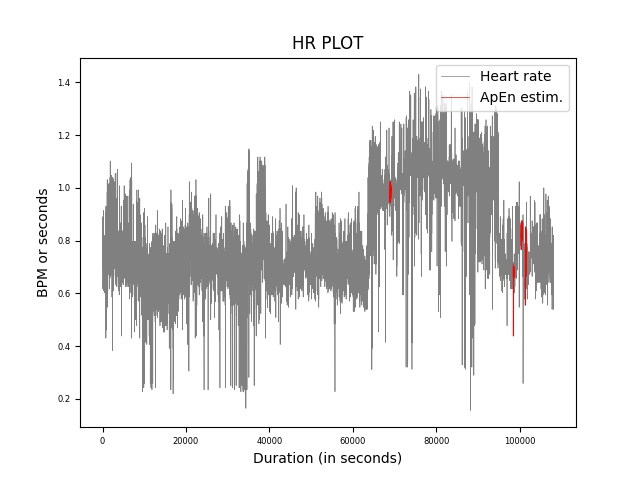
\includegraphics[width=.24\textwidth]{ApEn-long-term-af-db/long-term-af-database-1.0.0_19_240sec.jpeg}\hfill
		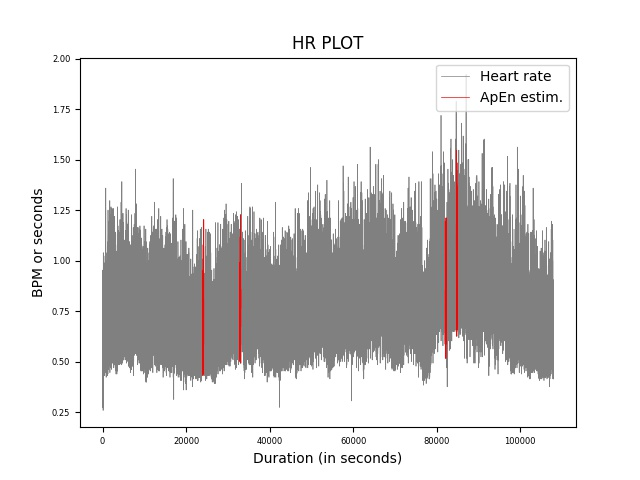
\includegraphics[width=.24\textwidth]{ApEn-long-term-af-db/long-term-af-database-1.0.0_20_240sec.jpeg}\hfill
		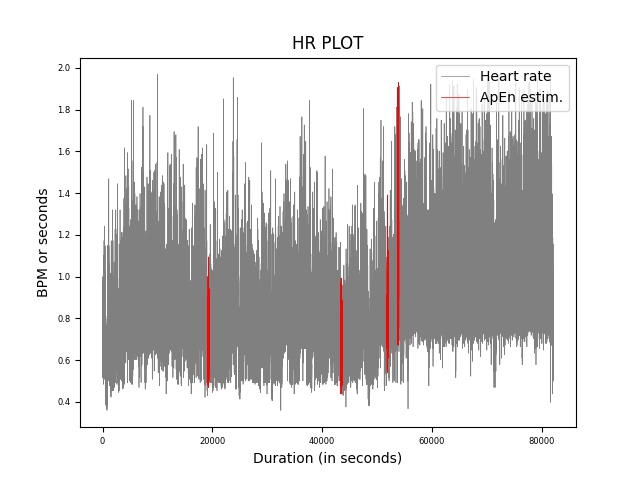
\includegraphics[width=.24\textwidth]{ApEn-long-term-af-db/long-term-af-database-1.0.0_21_240sec.jpeg}\hfill
		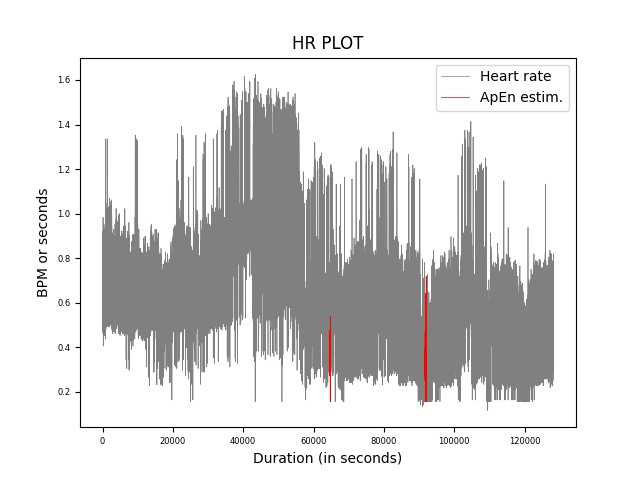
\includegraphics[width=.24\textwidth]{ApEn-long-term-af-db/long-term-af-database-1.0.0_22_240sec.jpeg}\hfill
		\\[\smallskipamount]
		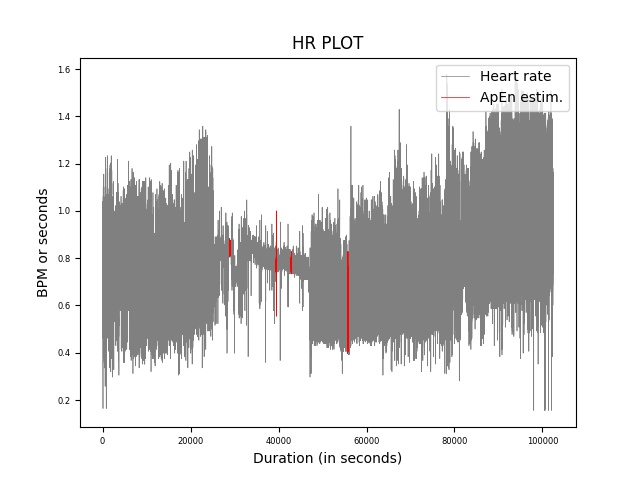
\includegraphics[width=.24\textwidth]{ApEn-long-term-af-db/long-term-af-database-1.0.0_23_240sec.jpeg}\hfill
		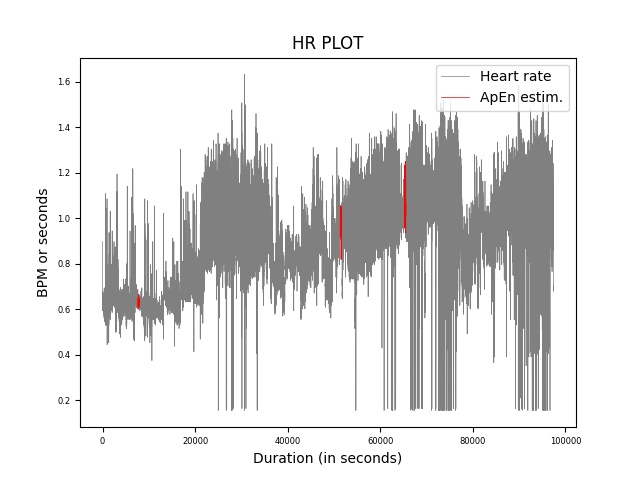
\includegraphics[width=.24\textwidth]{ApEn-long-term-af-db/long-term-af-database-1.0.0_24_240sec.jpeg}\hfill
		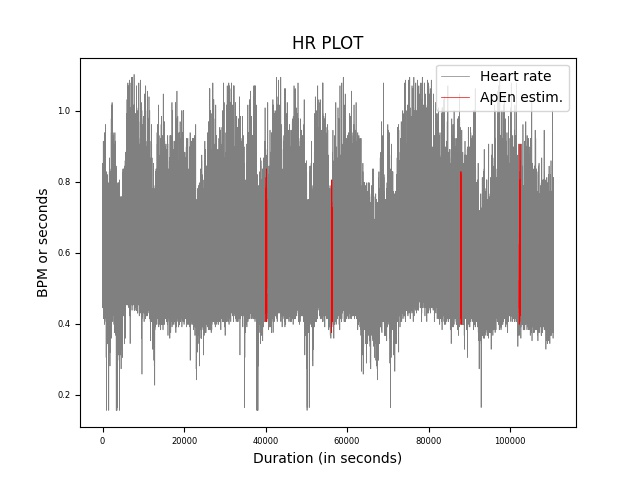
\includegraphics[width=.24\textwidth]{ApEn-long-term-af-db/long-term-af-database-1.0.0_25_240sec.jpeg}\hfill
		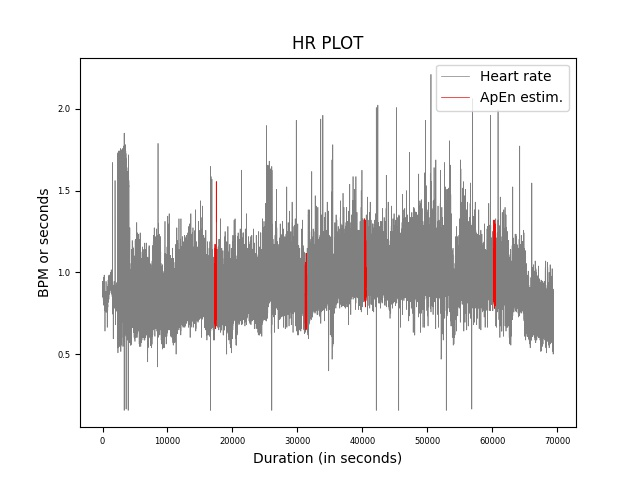
\includegraphics[width=.24\textwidth]{ApEn-long-term-af-db/long-term-af-database-1.0.0_26_240sec.jpeg}\hfill
		\caption{Συλλογή αποτελεσμάτων από τη βιβλιοθήκη \en Long Term AF Database \gr για τη μετρική \en ApEn \gr)}
	\end{figure}
	\item \en AVG: \gr Η συγκεκριμένη μέθοδος σε αντίθεση με την προηγούμενη έχει πιο εύστοχα αποτελέσματα και μεγαλύτερη σταθερότητα (Σχήμα 4.15). Υπάρχουν περιπτώσεις στις οποίες οι εκτιμήσεις ταυτίζονται με περιοχές-παλμούς με μη φυσιολογική καρδιακή λειτουργία, εξαιτίας της μορφολογίας του σήματος δεν είναι επιτυχείς (Σχήμα 4.16).
	\begin{figure}
		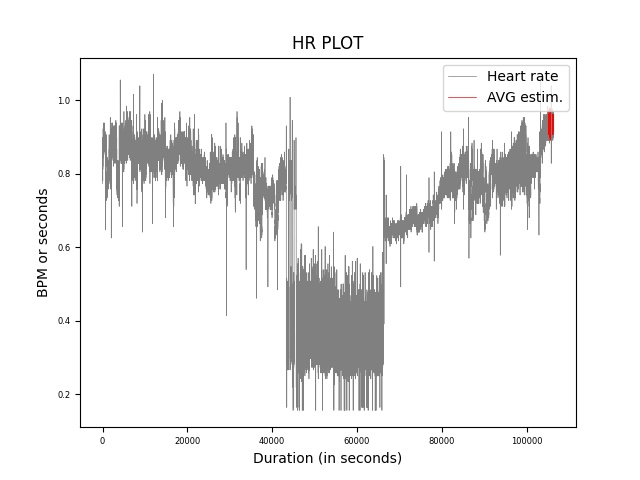
\includegraphics[width=.24\textwidth]{AVG-long-term-af-db/long-term-af-database-1.0.0_00_60sec.jpeg}\hfill
		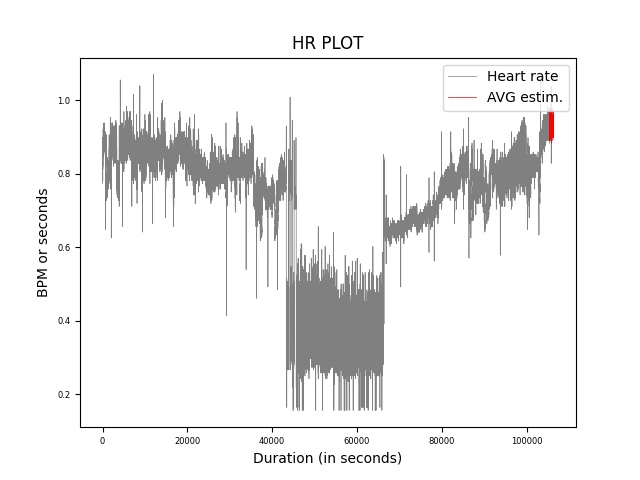
\includegraphics[width=.24\textwidth]{AVG-long-term-af-db/long-term-af-database-1.0.0_00_120sec.jpeg}\hfill
		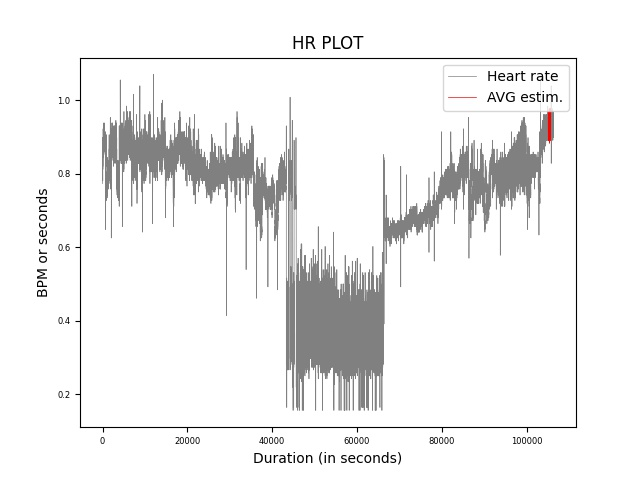
\includegraphics[width=.24\textwidth]{AVG-long-term-af-db/long-term-af-database-1.0.0_00_180sec.jpeg}\hfill
		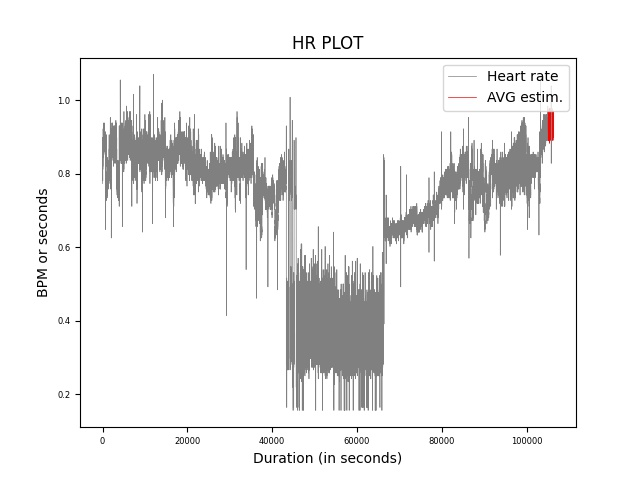
\includegraphics[width=.24\textwidth]{AVG-long-term-af-db/long-term-af-database-1.0.0_00_240sec.jpeg}\hfill
		\centering
		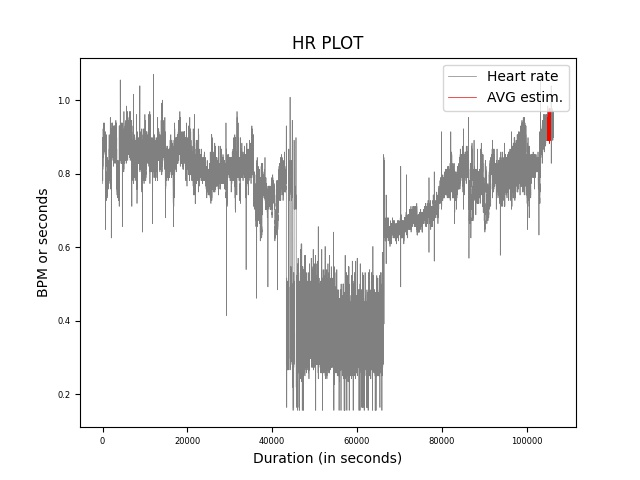
\includegraphics[width=.24\textwidth]{AVG-long-term-af-db/long-term-af-database-1.0.0_00_300sec.jpeg}\hfill
		\caption{Συλλογή αποτελεσμάτων από τη βιβλιοθήκη \en Long Term AF Database \gr για τη μετρική \en AVG \gr (αλλαγή μεγέθους παραθύρων)}
	\end{figure}
	\begin{figure}
		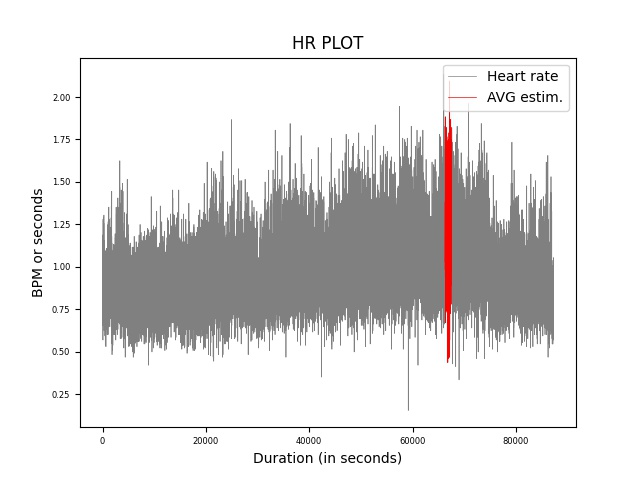
\includegraphics[width=.24\textwidth]{AVG-long-term-af-db/long-term-af-database-1.0.0_15_300sec.jpeg}\hfill
		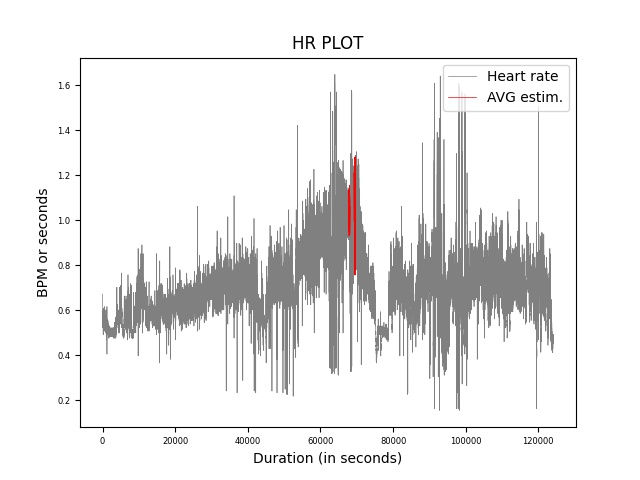
\includegraphics[width=.24\textwidth]{AVG-long-term-af-db/long-term-af-database-1.0.0_16_300sec.jpeg}\hfill
		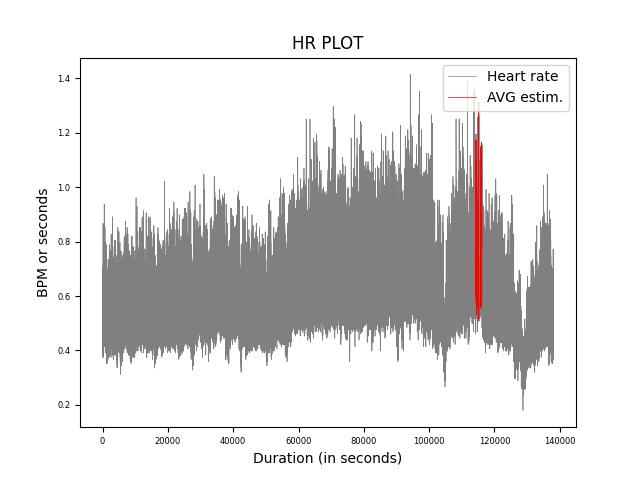
\includegraphics[width=.24\textwidth]{AVG-long-term-af-db/long-term-af-database-1.0.0_17_300sec.jpeg}\hfill
		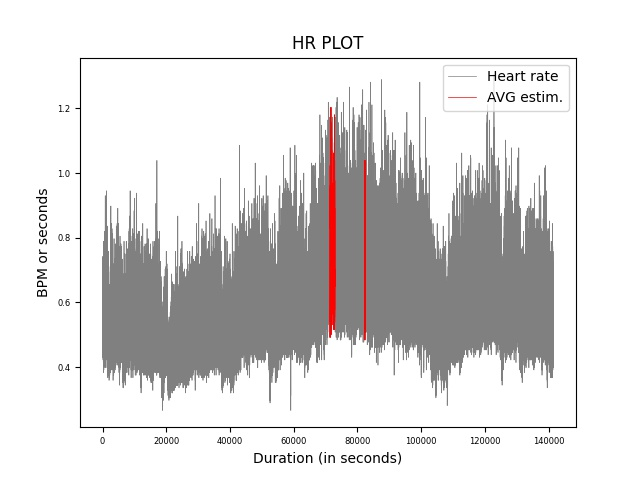
\includegraphics[width=.24\textwidth]{AVG-long-term-af-db/long-term-af-database-1.0.0_18_300sec.jpeg}\hfill
		\\[\smallskipamount]
		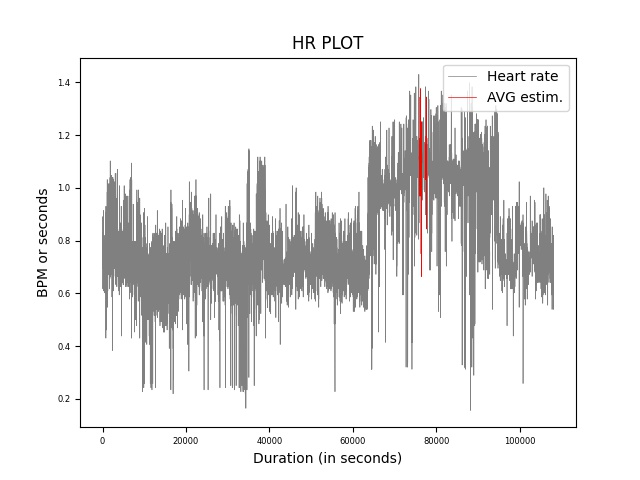
\includegraphics[width=.24\textwidth]{AVG-long-term-af-db/long-term-af-database-1.0.0_19_300sec.jpeg}\hfill
		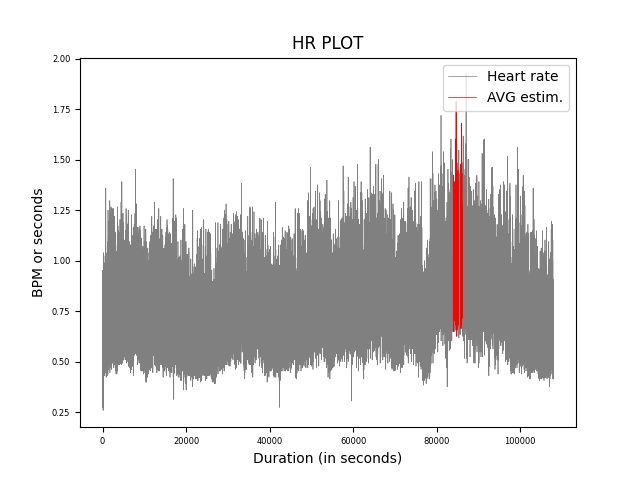
\includegraphics[width=.24\textwidth]{AVG-long-term-af-db/long-term-af-database-1.0.0_20_300sec.jpeg}\hfill
		\includegraphics[width=.24\textwidth]{AVG-long-term-af-db/long-term-af-database-1.0.0_21_300sec.jpeg}\hfill
		\includegraphics[width=.24\textwidth]{AVG-long-term-af-db/long-term-af-database-1.0.0_22_300sec.jpeg}\hfill
		\\[\smallskipamount]
		\includegraphics[width=.24\textwidth]{AVG-long-term-af-db/long-term-af-database-1.0.0_23_300sec.jpeg}\hfill
		\includegraphics[width=.24\textwidth]{AVG-long-term-af-db/long-term-af-database-1.0.0_24_300sec.jpeg}\hfill
		\includegraphics[width=.24\textwidth]{AVG-long-term-af-db/long-term-af-database-1.0.0_25_300sec.jpeg}\hfill
		\includegraphics[width=.24\textwidth]{AVG-long-term-af-db/long-term-af-database-1.0.0_26_300sec.jpeg}\hfill
		\caption{Συλλογή αποτελεσμάτων από τη βιβλιοθήκη \en Long Term AF Database \gr για τη μετρική \en AVG \gr)}
	\end{figure}
	\item  \en Bubble: \gr Σε αντίθεση με την \en ApEn \gr σε αυτή τη μέθοδο παρατηρείται πως όσο το μέγεθος του παραθύρου αυξάνεται, οι προβλέψεις του αλγορίθμου γίνονται πιο εύστοχες (Σχήμα 4.17), χωρίς αυτό να αναιρεί τη μη σταθερότητα της μεθόδου με την αλλαγή των μεγεθών σε κάθε δείγμα. Παρόλα αυτά τα αποτελέσματα είναι πιο ενθαρρυντικά (Σχήμα 4.18). 
	\begin{figure}
		\includegraphics[width=.24\textwidth]{Bubble-long-term-af-db/long-term-af-database-1.0.0_00_60sec.jpeg}\hfill
		\includegraphics[width=.24\textwidth]{Bubble-long-term-af-db/long-term-af-database-1.0.0_00_120sec.jpeg}\hfill
		\includegraphics[width=.24\textwidth]{Bubble-long-term-af-db/long-term-af-database-1.0.0_00_180sec.jpeg}\hfill
		\includegraphics[width=.24\textwidth]{Bubble-long-term-af-db/long-term-af-database-1.0.0_00_240sec.jpeg}\hfill
		\centering
		\includegraphics[width=.24\textwidth]{Bubble-long-term-af-db/long-term-af-database-1.0.0_00_300sec.jpeg}\hfill
		\caption{Συλλογή αποτελεσμάτων από τη βιβλιοθήκη \en Long Term AF Database \gr για τη μετρική \en Bubble \gr (αλλαγή μεγέθους παραθύρων)}
	\end{figure}
	\begin{figure}
		\includegraphics[width=.24\textwidth]{Bubble-long-term-af-db/long-term-af-database-1.0.0_15_240sec.jpeg}\hfill
		\includegraphics[width=.24\textwidth]{Bubble-long-term-af-db/long-term-af-database-1.0.0_16_240sec.jpeg}\hfill
		\includegraphics[width=.24\textwidth]{Bubble-long-term-af-db/long-term-af-database-1.0.0_17_240sec.jpeg}\hfill
		\includegraphics[width=.24\textwidth]{Bubble-long-term-af-db/long-term-af-database-1.0.0_18_240sec.jpeg}\hfill
		\\[\smallskipamount]
		\includegraphics[width=.24\textwidth]{Bubble-long-term-af-db/long-term-af-database-1.0.0_19_240sec.jpeg}\hfill
		\includegraphics[width=.24\textwidth]{Bubble-long-term-af-db/long-term-af-database-1.0.0_20_240sec.jpeg}\hfill
		\includegraphics[width=.24\textwidth]{Bubble-long-term-af-db/long-term-af-database-1.0.0_21_240sec.jpeg}\hfill
		\includegraphics[width=.24\textwidth]{Bubble-long-term-af-db/long-term-af-database-1.0.0_22_240sec.jpeg}\hfill
		\\[\smallskipamount]
		\includegraphics[width=.24\textwidth]{Bubble-long-term-af-db/long-term-af-database-1.0.0_23_240sec.jpeg}\hfill
		\includegraphics[width=.24\textwidth]{Bubble-long-term-af-db/long-term-af-database-1.0.0_24_240sec.jpeg}\hfill
		\includegraphics[width=.24\textwidth]{Bubble-long-term-af-db/long-term-af-database-1.0.0_25_240sec.jpeg}\hfill
		\includegraphics[width=.24\textwidth]{Bubble-long-term-af-db/long-term-af-database-1.0.0_26_240sec.jpeg}\hfill
		\caption{Συλλογή αποτελεσμάτων από τη βιβλιοθήκη \en Long Term AF Database \gr για τη μετρική \en Bubble \gr)}
	\end{figure}
	\item \en Rényi: \gr Η απόδοση αυτής της μετρικής θεωρείται μέτρια. Αυτό αιτιολογείται από τη μορφολογία του σήματος. Ενώ εντοπίζονται περιοχές που χαρακτηρίζονται ως μη φυσιολογικές, τα δείγματα βρίσκονται πολύ συχνά σε παρόμοια κατάσταση με αποτέλεσμα να μην εντοπίζονται οι πιο ακραίες από τις περιοχές. Αυτό που παρατηρείται είναι η εστίαση της μετρικής στις περιοχές με τις χαμηλότερες αριθμητικά τιμές και όχι στις υψηλές (Σχήματα 4.19, 4.20). 
	\begin{figure}
		\includegraphics[width=.24\textwidth]{Renyi-long-term-af/long-term-af-database-1.0.0_01_60sec.jpeg}\hfill
		\includegraphics[width=.24\textwidth]{Renyi-long-term-af/long-term-af-database-1.0.0_01_120sec.jpeg}\hfill
		\includegraphics[width=.24\textwidth]{Renyi-long-term-af/long-term-af-database-1.0.0_01_180sec.jpeg}\hfill
		\includegraphics[width=.24\textwidth]{Renyi-long-term-af/long-term-af-database-1.0.0_01_240sec.jpeg}\hfill
		\centering
		\includegraphics[width=.24\textwidth]{Renyi-long-term-af/long-term-af-database-1.0.0_01_300sec.jpeg}\hfill
		\caption{Συλλογή αποτελεσμάτων από τη βιβλιοθήκη \en Long Term AF Database \gr για τη μετρική \en Rényi \gr (αλλαγή μεγέθους παραθύρων)}
	\end{figure}
	\begin{figure}
		\includegraphics[width=.24\textwidth]{Renyi-long-term-af/long-term-af-database-1.0.0_00_300sec.jpeg}\hfill
		\includegraphics[width=.24\textwidth]{Renyi-long-term-af/long-term-af-database-1.0.0_105_240sec.jpeg}\hfill
		\includegraphics[width=.24\textwidth]{Renyi-long-term-af/long-term-af-database-1.0.0_116_300sec.jpeg}\hfill
		\includegraphics[width=.24\textwidth]{Renyi-long-term-af/long-term-af-database-1.0.0_119_240sec.jpeg}\hfill
		\includegraphics[width=.24\textwidth]{Renyi-long-term-af/long-term-af-database-1.0.0_120_300sec.jpeg}\hfill
		\\[\smallskipamount]
		\includegraphics[width=.24\textwidth]{Renyi-long-term-af/long-term-af-database-1.0.0_201_180sec.jpeg}\hfill
		\includegraphics[width=.24\textwidth]{Renyi-long-term-af/long-term-af-database-1.0.0_05_60sec.jpeg}\hfill
		\includegraphics[width=.24\textwidth]{Renyi-long-term-af/long-term-af-database-1.0.0_74_60sec.jpeg}\hfill
		\includegraphics[width=.24\textwidth]{Renyi-long-term-af/long-term-af-database-1.0.0_00_300sec.jpeg}\hfill
		\\[\smallskipamount]
		\includegraphics[width=.24\textwidth]{Renyi-long-term-af/long-term-af-database-1.0.0_08_120sec.jpeg}\hfill
		\includegraphics[width=.24\textwidth]{Renyi-long-term-af/long-term-af-database-1.0.0_122_60sec.jpeg}\hfill
		\includegraphics[width=.24\textwidth]{Renyi-long-term-af/long-term-af-database-1.0.0_206_60sec.jpeg}\hfill
		\includegraphics[width=.24\textwidth]{Renyi-long-term-af/long-term-af-database-1.0.0_208_300sec.jpeg}\hfill
		\caption{Συλλογή αποτελεσμάτων από τη βιβλιοθήκη \en Long Term AF Database \gr για τη μετρική \en Rényi \gr)}
	\end{figure}
	
	\item \en RMSSD: \gr Ίσως η μετρική με τα καλύτερα αποτελέσματα. Σταθερή όσο τα μεγέθη παραθύρων αλλάζουν (συγκλίνουν στις περισσότερες περιπτώσεις στην ίδια περιοχή εκτίμησης) και στην πλειοψηφία των δειγμάτων εντοπίζονται οι περιοχές με μεγαλύτερη πιθανότητα μη φυσιολογικής καρδιακής δραστηριότητας, αν και αυτό δε σημαίνει πολλά, λόγω της μόνιμης κατάστασης του σήματος. Ενδεικτικά αποτελέσματα των εκτιμήσεων αυτής της μετρικής εμφανίζονται στα Σχήματα 4.21, 4.22.
	
	\begin{figure}
		\includegraphics[width=.24\textwidth]{RMSSD-long-term-af-db/long-term-af-database-1.0.0_00_60sec.jpeg}\hfill
		\includegraphics[width=.24\textwidth]{RMSSD-long-term-af-db/long-term-af-database-1.0.0_00_120sec.jpeg}\hfill
		\includegraphics[width=.24\textwidth]{RMSSD-long-term-af-db/long-term-af-database-1.0.0_00_180sec.jpeg}\hfill
		\includegraphics[width=.24\textwidth]{RMSSD-long-term-af-db/long-term-af-database-1.0.0_00_240sec.jpeg}\hfill
		\centering
		\includegraphics[width=.24\textwidth]{RMSSD-long-term-af-db/long-term-af-database-1.0.0_00_300sec.jpeg}\hfill
		\caption{Συλλογή αποτελεσμάτων από τη βιβλιοθήκη \en Long Term AF Database \gr για τη μετρική \en RMSSD \gr (αλλαγή μεγέθους παραθύρων)}
	\end{figure}
	\begin{figure}
		\includegraphics[width=.24\textwidth]{RMSSD-long-term-af-db/long-term-af-database-1.0.0_15_240sec.jpeg}\hfill
		\includegraphics[width=.24\textwidth]{RMSSD-long-term-af-db/long-term-af-database-1.0.0_16_240sec.jpeg}\hfill
		\includegraphics[width=.24\textwidth]{RMSSD-long-term-af-db/long-term-af-database-1.0.0_17_240sec.jpeg}\hfill
		\includegraphics[width=.24\textwidth]{RMSSD-long-term-af-db/long-term-af-database-1.0.0_18_240sec.jpeg}\hfill
		\\[\smallskipamount]
		\includegraphics[width=.24\textwidth]{RMSSD-long-term-af-db/long-term-af-database-1.0.0_19_240sec.jpeg}\hfill
		\includegraphics[width=.24\textwidth]{RMSSD-long-term-af-db/long-term-af-database-1.0.0_20_240sec.jpeg}\hfill
		\includegraphics[width=.24\textwidth]{RMSSD-long-term-af-db/long-term-af-database-1.0.0_21_240sec.jpeg}\hfill
		\includegraphics[width=.24\textwidth]{RMSSD-long-term-af-db/long-term-af-database-1.0.0_22_240sec.jpeg}\hfill
		\\[\smallskipamount]
		\includegraphics[width=.24\textwidth]{RMSSD-long-term-af-db/long-term-af-database-1.0.0_23_240sec.jpeg}\hfill
		\includegraphics[width=.24\textwidth]{RMSSD-long-term-af-db/long-term-af-database-1.0.0_24_240sec.jpeg}\hfill
		\includegraphics[width=.24\textwidth]{RMSSD-long-term-af-db/long-term-af-database-1.0.0_25_240sec.jpeg}\hfill
		\includegraphics[width=.24\textwidth]{RMSSD-long-term-af-db/long-term-af-database-1.0.0_26_240sec.jpeg}\hfill
		\caption{Συλλογή αποτελεσμάτων από τη βιβλιοθήκη \en Long Term AF Database \gr για τη μετρική \en RMSSD \gr)}
	\end{figure}
	
	\item \en SampEn: \gr Η εικόνα που αποδίδει παραπέμπει στην εικόνα της \en ApEn \gr με την ίδια αστάθεια και άστοχη εκτίμηση. Αυτή η διαπίστωση είναι κάτι που εύκολα διακρίνεται και "με το μάτι" από τα αποτελέσματα των διαγραμμάτων στα Σχήματα 4.23, 4.24.
	
	
	\begin{figure}
		\includegraphics[width=.24\textwidth]{SampEn-long-term-af-db/long-term-af-database-1.0.0_00_60sec.jpeg}\hfill
		\includegraphics[width=.24\textwidth]{SampEn-long-term-af-db/long-term-af-database-1.0.0_00_120sec.jpeg}\hfill
		\includegraphics[width=.24\textwidth]{SampEn-long-term-af-db/long-term-af-database-1.0.0_00_180sec.jpeg}\hfill
		\includegraphics[width=.24\textwidth]{SampEn-long-term-af-db/long-term-af-database-1.0.0_00_240sec.jpeg}\hfill
		\centering
		\includegraphics[width=.24\textwidth]{SampEn-long-term-af-db/long-term-af-database-1.0.0_00_300sec.jpeg}\hfill
		\caption{Συλλογή αποτελεσμάτων από τη βιβλιοθήκη \en Long Term AF Database \gr για τη μετρική \en SampEn \gr (αλλαγή μεγέθους παραθύρων)}
	\end{figure}
	\begin{figure}
		\includegraphics[width=.24\textwidth]{SampEn-long-term-af-db/long-term-af-database-1.0.0_15_300sec.jpeg}\hfill
		\includegraphics[width=.24\textwidth]{SampEn-long-term-af-db/long-term-af-database-1.0.0_16_300sec.jpeg}\hfill
		\includegraphics[width=.24\textwidth]{SampEn-long-term-af-db/long-term-af-database-1.0.0_17_300sec.jpeg}\hfill
		\includegraphics[width=.24\textwidth]{SampEn-long-term-af-db/long-term-af-database-1.0.0_18_300sec.jpeg}\hfill
		\\[\smallskipamount]
		\includegraphics[width=.24\textwidth]{SampEn-long-term-af-db/long-term-af-database-1.0.0_19_300sec.jpeg}\hfill
		\includegraphics[width=.24\textwidth]{SampEn-long-term-af-db/long-term-af-database-1.0.0_20_300sec.jpeg}\hfill
		\includegraphics[width=.24\textwidth]{SampEn-long-term-af-db/long-term-af-database-1.0.0_21_300sec.jpeg}\hfill
		\includegraphics[width=.24\textwidth]{SampEn-long-term-af-db/long-term-af-database-1.0.0_22_300sec.jpeg}\hfill
		\\[\smallskipamount]
		\includegraphics[width=.24\textwidth]{SampEn-long-term-af-db/long-term-af-database-1.0.0_23_300sec.jpeg}\hfill
		\includegraphics[width=.24\textwidth]{SampEn-long-term-af-db/long-term-af-database-1.0.0_24_300sec.jpeg}\hfill
		\includegraphics[width=.24\textwidth]{SampEn-long-term-af-db/long-term-af-database-1.0.0_25_300sec.jpeg}\hfill
		\includegraphics[width=.24\textwidth]{SampEn-long-term-af-db/long-term-af-database-1.0.0_26_300sec.jpeg}\hfill
		\caption{Συλλογή αποτελεσμάτων από τη βιβλιοθήκη \en Long Term AF Database \gr για τη μετρική \en SampEn \gr)}
	\end{figure}
	
	\item \en Shannon: \gr Τα αποτελέσματα εκτίμησης αυτής της μεθόδου βρίσκονται σε μία μέση κατάσταση. Υπάρχουν τόσο δείγματα που εντοπίζουν παλμούς με πολύ υψηλές τιμές όσο και περιπτώσεις που οι εκτιμήσεις είναι εντελώς άστοχες. Ακόμα, η μέθοδος συγκλίνει στις περισσότερες περιπτώσεις στην ίδια περιοχή, ανεξαρτήτως του μεγέθους του παραθύρου (Σχήμα 4.25, Σχήμα 4.26). 
	
	\begin{figure}
		\includegraphics[width=.24\textwidth]{Shannon-long-term-af-db/long-term-af-database-1.0.0_15_60sec.jpeg}\hfill
		\includegraphics[width=.24\textwidth]{Shannon-long-term-af-db/long-term-af-database-1.0.0_15_120sec.jpeg}\hfill
		\includegraphics[width=.24\textwidth]{Shannon-long-term-af-db/long-term-af-database-1.0.0_15_180sec.jpeg}\hfill
		\includegraphics[width=.24\textwidth]{Shannon-long-term-af-db/long-term-af-database-1.0.0_15_240sec.jpeg}\hfill
		\centering
		\includegraphics[width=.24\textwidth]{Shannon-long-term-af-db/long-term-af-database-1.0.0_15_300sec.jpeg}\hfill
		\caption{Συλλογή αποτελεσμάτων από τη βιβλιοθήκη \en Long Term AF Database \gr για τη μετρική \en Shannon \gr (αλλαγή μεγέθους παραθύρων)}
	\end{figure}
	\begin{figure}
		\includegraphics[width=.24\textwidth]{Shannon-long-term-af-db/long-term-af-database-1.0.0_15_120sec.jpeg}\hfill
		\includegraphics[width=.24\textwidth]{Shannon-long-term-af-db/long-term-af-database-1.0.0_16_120sec.jpeg}\hfill
		\includegraphics[width=.24\textwidth]{Shannon-long-term-af-db/long-term-af-database-1.0.0_17_120sec.jpeg}\hfill
		\includegraphics[width=.24\textwidth]{Shannon-long-term-af-db/long-term-af-database-1.0.0_18_120sec.jpeg}\hfill
		\\[\smallskipamount]
		\includegraphics[width=.24\textwidth]{Shannon-long-term-af-db/long-term-af-database-1.0.0_19_120sec.jpeg}\hfill
		\includegraphics[width=.24\textwidth]{Shannon-long-term-af-db/long-term-af-database-1.0.0_20_120sec.jpeg}\hfill
		\includegraphics[width=.24\textwidth]{Shannon-long-term-af-db/long-term-af-database-1.0.0_21_120sec.jpeg}\hfill
		\includegraphics[width=.24\textwidth]{Shannon-long-term-af-db/long-term-af-database-1.0.0_22_120sec.jpeg}\hfill
		\\[\smallskipamount]
		\includegraphics[width=.24\textwidth]{Shannon-long-term-af-db/long-term-af-database-1.0.0_23_120sec.jpeg}\hfill
		\includegraphics[width=.24\textwidth]{Shannon-long-term-af-db/long-term-af-database-1.0.0_24_120sec.jpeg}\hfill
		\includegraphics[width=.24\textwidth]{Shannon-long-term-af-db/long-term-af-database-1.0.0_25_120sec.jpeg}\hfill
		\includegraphics[width=.24\textwidth]{Shannon-long-term-af-db/long-term-af-database-1.0.0_26_120sec.jpeg}\hfill
		\caption{Συλλογή αποτελεσμάτων από τη βιβλιοθήκη \en Long Term AF Database \gr για τη μετρική \en Shannon \gr)}
	\end{figure}
	\en
	\item STD:\gr Μία ακόμη μετρική με αρκετά εύστοχα αποτελέσματα, παραπέμπει στις εκτιμήσεις της \en RMSSD \gr με αρκετά μεγάλη σταθερότητα και ευστοχία (Σχήμα 4.27, Σχήμα 4.28).
	\begin{figure}
		\includegraphics[width=.24\textwidth]{STD-long-term-af-db/long-term-af-database-1.0.0_15_60sec.jpeg}\hfill
		\includegraphics[width=.24\textwidth]{STD-long-term-af-db/long-term-af-database-1.0.0_15_120sec.jpeg}\hfill
		\includegraphics[width=.24\textwidth]{STD-long-term-af-db/long-term-af-database-1.0.0_15_180sec.jpeg}\hfill
		\includegraphics[width=.24\textwidth]{STD-long-term-af-db/long-term-af-database-1.0.0_15_240sec.jpeg}\hfill
		\centering
		\includegraphics[width=.24\textwidth]{STD-long-term-af-db/long-term-af-database-1.0.0_15_300sec.jpeg}\hfill
		\caption{Συλλογή αποτελεσμάτων από τη βιβλιοθήκη \en Long Term AF Database \gr για τη μετρική \en STD \gr (αλλαγή μεγέθους παραθύρων)}
	\end{figure}
	\begin{figure}
		\includegraphics[width=.24\textwidth]{STD-long-term-af-db/long-term-af-database-1.0.0_15_300sec.jpeg}\hfill
		\includegraphics[width=.24\textwidth]{STD-long-term-af-db/long-term-af-database-1.0.0_16_300sec.jpeg}\hfill
		\includegraphics[width=.24\textwidth]{STD-long-term-af-db/long-term-af-database-1.0.0_17_300sec.jpeg}\hfill
		\includegraphics[width=.24\textwidth]{STD-long-term-af-db/long-term-af-database-1.0.0_18_300sec.jpeg}\hfill
		\\[\smallskipamount]
		\includegraphics[width=.24\textwidth]{STD-long-term-af-db/long-term-af-database-1.0.0_19_300sec.jpeg}\hfill
		\includegraphics[width=.24\textwidth]{STD-long-term-af-db/long-term-af-database-1.0.0_20_300sec.jpeg}\hfill
		\includegraphics[width=.24\textwidth]{STD-long-term-af-db/long-term-af-database-1.0.0_21_300sec.jpeg}\hfill
		\includegraphics[width=.24\textwidth]{STD-long-term-af-db/long-term-af-database-1.0.0_22_300sec.jpeg}\hfill
		\\[\smallskipamount]
		\includegraphics[width=.24\textwidth]{STD-long-term-af-db/long-term-af-database-1.0.0_23_300sec.jpeg}\hfill
		\includegraphics[width=.24\textwidth]{STD-long-term-af-db/long-term-af-database-1.0.0_24_300sec.jpeg}\hfill
		\includegraphics[width=.24\textwidth]{STD-long-term-af-db/long-term-af-database-1.0.0_25_300sec.jpeg}\hfill
		\includegraphics[width=.24\textwidth]{STD-long-term-af-db/long-term-af-database-1.0.0_26_300sec.jpeg}\hfill
		\caption{Συλλογή αποτελεσμάτων από τη βιβλιοθήκη \en Long Term AF Database \gr για τη μετρική \en STD \gr)}
	\end{figure}
	
	\item \en Haar wavelets: \gr Μια συνοπτική εικόνα για όλες τις κλίμακες των κυματιδίων (από κλίμακα 2 έως και 10) οδηγεί στο συμπέρασμα πως μπορούν να εντοπίσουν περιοχές που μπορούν πιθανώς να αποβούν επικίνδυνες στις περιπτώσεις που το καρδιογράφημα το επιτρέπει. Στα δείγματα των οποίων το σήμα βρισκόταν σε μόνιμη μη φυσιολογική κατάσταση, όπως και με τις προηγούμενες μετρικές, τα κυματίδια δε δείχουν τα ίδια αποτελέσματα. Όσο ο βαθμός της κλίμακας αυξάνεται, οι εκτιμήσεις φαίνεται να συγκλίνουν η μια στην άλλη και το ίδιο ισχύει για το μέγεθος του παραθύρου. Παραδείγματος χάριν, για μια συγκεκριμένη καταγραφή, στην κλίμακα 2 όσο το μέγεθος του παραθύρου αυξάνεται οι εκτιμήσεις δεν αποκλίνουν ιδιαίτερα η μία από την άλλη. Αντίθετα, φαίνεται να υπάρχει μια σύγκλιση. Η διαδικασία αυτή επαναλαμβάνεται για την πλειοψηφία των υπόλοιπων μεγεθών, τόσο για την κλίμακα εκτίμησης όσο και για τα μεγέθη των παραθύρων (Σχήμα 4.29). Μιας και οι περιοχές που εντοπίζονται από τα κυματίδια είναι σε μεγάλη πλειοψηφία παρόμοια ή πανομοιότυπα η απεικόνιση των εκτιμήσεων κατά τη μεταβολή των παραθύρων παραλείπεται (όταν η κλίμακα ισοδυναμεί με 10 οι εκτιμήσεις μεταβάλλονται ελάχιστα).
	
	\begin{figure}
		\centering
		\includegraphics[width=.24\textwidth]{Haar-long-term-af/Haar_scale_2_01_180sec.jpeg}\hfill
		\includegraphics[width=.24\textwidth]{Haar-long-term-af/Haar_scale_2_03_300sec.jpeg}\hfill
		\includegraphics[width=.24\textwidth]{Haar-long-term-af/Haar_scale_3_06_300sec.jpeg}\hfill
		\\[\smallskipamount]
		\includegraphics[width=.24\textwidth]{Haar-long-term-af/Haar_scale_3_08_240sec.jpeg}\hfill
		\includegraphics[width=.24\textwidth]{Haar-long-term-af/Haar_scale_4_15_60sec.jpeg}\hfill
		\includegraphics[width=.24\textwidth]{Haar-long-term-af/Haar_scale_4_16_180sec.jpeg}\hfill
		\includegraphics[width=.24\textwidth]{Haar-long-term-af/Haar_scale_5_16_180sec.jpeg}\hfill
		\\[\smallskipamount]
		\includegraphics[width=.24\textwidth]{Haar-long-term-af/Haar_scale_5_21_300sec.jpeg}\hfill
		\includegraphics[width=.24\textwidth]{Haar-long-term-af/Haar_scale_6_25_300sec.jpeg}\hfill
		\includegraphics[width=.24\textwidth]{Haar-long-term-af/Haar_scale_6_26_180sec.jpeg}\hfill
		\includegraphics[width=.24\textwidth]{Haar-long-term-af/Haar_scale_7_28_120sec.jpeg}\hfill
		\\[\smallskipamount]
		\includegraphics[width=.24\textwidth]{Haar-long-term-af/Haar_scale_7_30_180sec.jpeg}\hfill
		\includegraphics[width=.24\textwidth]{Haar-long-term-af/Haar_scale_8_68_300sec.jpeg}\hfill
		\includegraphics[width=.24\textwidth]{Haar-long-term-af/Haar_scale_8_68_300sec.jpeg}\hfill
		\includegraphics[width=.24\textwidth]{Haar-long-term-af/Haar_scale_9_103_120sec.jpeg}\hfill
		\\[\smallskipamount]
		\centering
		\includegraphics[width=.24\textwidth]{Haar-long-term-af/Haar_scale_9_104_300sec.jpeg}\hfill
		\includegraphics[width=.24\textwidth]{Haar-long-term-af/Haar_scale_10_122_300sec.jpeg}\hfill
		\includegraphics[width=.24\textwidth]{Haar-long-term-af/Haar_scale_10_122_300sec.jpeg}\hfill
		\caption{Συλλογή αποτελεσμάτων από τη βιβλιοθήκη \en Long Term AF Database \gr για τα κυματίδια \en Haar \gr)}
	\end{figure}
	
\end{itemize}
\subsection{\en MIT-BIH Arrhythmia Database \gr}
Σε αυτή την περίπτωση, τα αποτελέσματα είναι αρκετά ενθαρρυντικά. Τα δείγματα της συγκεκριμένης βάσης δε διαθέτουν ιδιαίτερο θόρυβο και έντονες αυξομειώσεις. Για αυτόν ακριβώς το λόγο, στα δείγματα στα οποία δε βρίσκονται σε μόνιμη αταξία, ο αλγόριθμος εντοπίζει αρκετά εύκολα και συχνά τις περιοχές που αποκλίνουν και οδηγούν στην εικόνα της "επικίνδυνης" περιοχής. Παρόλα αυτά, υπάρχουν και αρκετά δείγματα τα οποία, ενώ δε βρίσκονται σε μόνιμη κατάσταση εκτός του φυσιολογικού και οι διαταραχές είναι περιορισμένες, όταν εμφανίζονται, διαρκούν μεγάλη χρονική περίοδο. Με αυτό τον τρόπο, ενώ οι περιοχές που εντοπίζονται από τον αλγόριθμο είναι σωστές, δεν είναι οι μόνες ούτε και οι πιο έντονες, δίνοντας την εικόνα μιας λανθασμένης εκτίμησης. Σαν γενικότερο σχόλιο επομένως μπορεί να σημειωθεί πως όταν τα δείγματα είναι πιο ευκρινή και λιγότερο άστατα, οι εκτιμήσεις των μετρικών είναι αναμενόμενα πιο ακριβείς. Τα μεγέθη παραθύρων που εξετάστηκαν ήταν τα [60, 120, 180, 240, 300] δευτερόλεπτα. Τα αρχικά δείγματα είχαν την εξής εικόνα (Σχήμα 4.30): 
\begin{figure}
	\includegraphics[width=.24\textwidth]{mitbih-arr-db/mit-bih-arrhythmia-database-1.0.0_116.png}\hfill
	\includegraphics[width=.24\textwidth]{mitbih-arr-db/mit-bih-arrhythmia-database-1.0.0_117.png}\hfill
	\includegraphics[width=.24\textwidth]{mitbih-arr-db/mit-bih-arrhythmia-database-1.0.0_119.png}\hfill
	\includegraphics[width=.24\textwidth]{mitbih-arr-db/mit-bih-arrhythmia-database-1.0.0_121.png}\hfill
	\\[\smallskipamount]
	\includegraphics[width=.24\textwidth]{mitbih-arr-db/mit-bih-arrhythmia-database-1.0.0_122.png}\hfill
	\includegraphics[width=.24\textwidth]{mitbih-arr-db/mit-bih-arrhythmia-database-1.0.0_207.png}\hfill
	\includegraphics[width=.24\textwidth]{mitbih-arr-db/mit-bih-arrhythmia-database-1.0.0_208.png}\hfill
	\includegraphics[width=.24\textwidth]{mitbih-arr-db/mit-bih-arrhythmia-database-1.0.0_209.png}\hfill
	\\[\smallskipamount]
	\includegraphics[width=.24\textwidth]{mitbih-arr-db/mit-bih-arrhythmia-database-1.0.0_210.png}\hfill
	\includegraphics[width=.24\textwidth]{mitbih-arr-db/mit-bih-arrhythmia-database-1.0.0_222.png}\hfill
	\includegraphics[width=.24\textwidth]{mitbih-arr-db/mit-bih-arrhythmia-database-1.0.0_223.png}\hfill
	\includegraphics[width=.24\textwidth]{mitbih-arr-db/mit-bih-arrhythmia-database-1.0.0_234.png}\hfill
	\caption{Συλλογή αποτελεσμάτων από τη βιβλιοθήκη \en MIT-BIH Arrhythmia Database \gr (αρχικά δείγματα/καταγραφές)}
\end{figure}
Μετά την εφαρμογή του αλγορίθμου τα αποτελέσματα ήταν τα:
\begin{itemize}
	\item \en ApEn: \gr Σε αυτή τη βιβλιοθήκη παρατηρείται το εξής· όσο πιο ακραίες είναι οι τιμές των παραθύρων (τα 60 δευτερόλεπτα ή τα 300 παραδείγματος χάριν) τόσο πιο έγκυρες είναι οι εκτιμήσεις του αλγόριθμου. Παρόλα αυτά, αν και αυτή η μέθοδος καταφέρνει να εντοπίσει περιοχές με μη φυσιολογική λειτουργία (πάντα σε σύγκριση με τη μέση λειτουργία και τιμές ολόκληρου του σήματος) δεν καταφέρνει σε αρκετές περιπτώσεις να εντοπίσει τις μέγιστες ή ελάχιστες τιμές. 
	Μερικά δείγματα των εκτιμήσεων της \en ApEn \gr παρουσιάζονται εδώ (Σχήμα 4.31, Σχήμα 4.32):
	\begin{figure}
		\includegraphics[width=.24\textwidth]{ApEn-mitbih-arr-db/mit-bih-arrhythmia-database-1.0.0_109_60sec.jpeg}\hfill
		\includegraphics[width=.24\textwidth]{ApEn-mitbih-arr-db/mit-bih-arrhythmia-database-1.0.0_109_120sec.jpeg}\hfill
		\includegraphics[width=.24\textwidth]{ApEn-mitbih-arr-db/mit-bih-arrhythmia-database-1.0.0_109_180sec.jpeg}\hfill
		\includegraphics[width=.24\textwidth]{ApEn-mitbih-arr-db/mit-bih-arrhythmia-database-1.0.0_109_240sec.jpeg}\hfill
		\centering
		\includegraphics[width=.24\textwidth]{ApEn-mitbih-arr-db/mit-bih-arrhythmia-database-1.0.0_109_300sec.jpeg}\hfill
		\caption{Συλλογή αποτελεσμάτων από τη βιβλιοθήκη \en MIT-BIH Arrhythmia Database \gr για τη μετρική \en ApEn \gr (αλλαγή μεγέθους παραθύρων)}
	\end{figure}
	\begin{figure}
		\includegraphics[width=.24\textwidth]{ApEn-mitbih-arr-db/mit-bih-arrhythmia-database-1.0.0_111_60sec.jpeg}\hfill
		\includegraphics[width=.24\textwidth]{ApEn-mitbih-arr-db/mit-bih-arrhythmia-database-1.0.0_116_180sec.jpeg}\hfill
		\includegraphics[width=.24\textwidth]{ApEn-mitbih-arr-db/mit-bih-arrhythmia-database-1.0.0_117_120sec.jpeg}\hfill
		\includegraphics[width=.24\textwidth]{ApEn-mitbih-arr-db/mit-bih-arrhythmia-database-1.0.0_121_60sec.jpeg}\hfill
		\\[\smallskipamount]
		\includegraphics[width=.24\textwidth]{ApEn-mitbih-arr-db/mit-bih-arrhythmia-database-1.0.0_122_300sec.jpeg}\hfill
		\includegraphics[width=.24\textwidth]{ApEn-mitbih-arr-db/mit-bih-arrhythmia-database-1.0.0_123_60sec.jpeg}\hfill
		\includegraphics[width=.24\textwidth]{ApEn-mitbih-arr-db/mit-bih-arrhythmia-database-1.0.0_202_60sec.jpeg}\hfill
		\includegraphics[width=.24\textwidth]{ApEn-mitbih-arr-db/mit-bih-arrhythmia-database-1.0.0_205_180sec.jpeg}\hfill
		\\[\smallskipamount]
		\includegraphics[width=.24\textwidth]{ApEn-mitbih-arr-db/mit-bih-arrhythmia-database-1.0.0_207_60sec.jpeg}\hfill
		\includegraphics[width=.24\textwidth]{ApEn-mitbih-arr-db/mit-bih-arrhythmia-database-1.0.0_208_240sec.jpeg}\hfill
		\includegraphics[width=.24\textwidth]{ApEn-mitbih-arr-db/mit-bih-arrhythmia-database-1.0.0_212_240sec.jpeg}\hfill
		\includegraphics[width=.24\textwidth]{ApEn-mitbih-arr-db/mit-bih-arrhythmia-database-1.0.0_215_300sec.jpeg}\hfill
		\caption{Συλλογή αποτελεσμάτων από τη βιβλιοθήκη \en MIT-BIH Arrhythmia Database \gr για τη μετρική \en ApEn \gr)}
	\end{figure}
	\item \en AVG: \gr Σε αντίθεση με την προηγούμενη βιβλιοθήκη, εδώ τα αποτελέσματα των εκτιμήσεων δεν είναι τόσο ικανοποιητικά. Το γεγονός ότι τα αποτελέσματά της παραμένουν σταθερά όσο το μέγεθος του παραθύρου αλλάζει (δηλαδή οι περιοχές που εκτιμώνται ως μη φυσιολογικές είναι παρόμοιες ανεξαρτήτως του μεγέθους του πραθύρου), πολλές φορές αποτελεί μειονέκτημα. Ενώ υπάρχουν καταγραφές στις οποίες τα αποτελέσματα είναι εύστοχα, δεν ισχύει το ίδιο για το σύνολο των σημάτων. Στη συνέχεια παρουσιάζονται ενδεικτικά μερικά από τα αποτελέσματα (Σχήμα 4.33, Σχήμα 4.34).
	
	\begin{figure}
		\includegraphics[width=.24\textwidth]{AVG-mitbih-arr-db/mit-bih-arrhythmia-database-1.0.0_104_60sec.jpeg}\hfill
		\includegraphics[width=.24\textwidth]{AVG-mitbih-arr-db/mit-bih-arrhythmia-database-1.0.0_104_120sec.jpeg}\hfill
		\includegraphics[width=.24\textwidth]{AVG-mitbih-arr-db/mit-bih-arrhythmia-database-1.0.0_104_180sec.jpeg}\hfill
		\includegraphics[width=.24\textwidth]{AVG-mitbih-arr-db/mit-bih-arrhythmia-database-1.0.0_104_240sec.jpeg}\hfill
		\centering
		\includegraphics[width=.24\textwidth]{AVG-mitbih-arr-db/mit-bih-arrhythmia-database-1.0.0_104_300sec.jpeg}\hfill
		\caption{Συλλογή αποτελεσμάτων από τη βιβλιοθήκη \en MIT-BIH Arrhythmia Database \gr για τη μετρική \en AVG \gr με αρνητικά αποτελέσματα (αλλαγή μεγέθους παραθύρων)}
	\end{figure}
	
	\begin{figure}
		\includegraphics[width=.24\textwidth]{AVG-mitbih-arr-db/mit-bih-arrhythmia-database-1.0.0_105_300sec.jpeg}\hfill
		\includegraphics[width=.24\textwidth]{AVG-mitbih-arr-db/mit-bih-arrhythmia-database-1.0.0_107_60sec.jpeg}\hfill
		\includegraphics[width=.24\textwidth]{AVG-mitbih-arr-db/mit-bih-arrhythmia-database-1.0.0_111_300sec.jpeg}\hfill
		\includegraphics[width=.24\textwidth]{AVG-mitbih-arr-db/mit-bih-arrhythmia-database-1.0.0_208_120sec.jpeg}\hfill
		\\[\smallskipamount]
		\includegraphics[width=.24\textwidth]{AVG-mitbih-arr-db/mit-bih-arrhythmia-database-1.0.0_212_180sec.jpeg}\hfill
		\includegraphics[width=.24\textwidth]{AVG-mitbih-arr-db/mit-bih-arrhythmia-database-1.0.0_219_180sec.jpeg}\hfill
		\includegraphics[width=.24\textwidth]{AVG-mitbih-arr-db/mit-bih-arrhythmia-database-1.0.0_221_120sec.jpeg}\hfill
		\includegraphics[width=.24\textwidth]{AVG-mitbih-arr-db/mit-bih-arrhythmia-database-1.0.0_222_180sec.jpeg}\hfill
		\\[\smallskipamount]
		\includegraphics[width=.24\textwidth]{AVG-mitbih-arr-db/mit-bih-arrhythmia-database-1.0.0_230_240sec.jpeg}\hfill
		\includegraphics[width=.24\textwidth]{AVG-mitbih-arr-db/mit-bih-arrhythmia-database-1.0.0_231_180sec.jpeg}\hfill
		\includegraphics[width=.24\textwidth]{AVG-mitbih-arr-db/mit-bih-arrhythmia-database-1.0.0_232_240sec.jpeg}\hfill
		\includegraphics[width=.24\textwidth]{AVG-mitbih-arr-db/mit-bih-arrhythmia-database-1.0.0_234_120sec.jpeg}\hfill
		\caption{Συλλογή αποτελεσμάτων από τη βιβλιοθήκη \en MIT-BIH Arrhythmia Database \gr για τη μετρική \en AVG \gr)}
	\end{figure}
	
	\item \en Bubble: \gr Όπως και στην προηγούμενη βιβλιοθήκη, τα αποτελέσματα αυτής της μεθόδου εκτίμησης εντροπίας είναι πιο αξιόπιστα σε σύγκριση με την \en ApEn \gr. Στις περισσότερες καταγραφές καταφέρνει να εντοπίσει περιοχές του σήματος που αποκλίνουν από τη φυσιολογική λειτουργία της καρδιάς (συχνά και τις πιο "έντονες" περιοχές του σήματος). Αν και τα αποτελέσματα εντοπισμού είναι αρκετά ευνοϊκά, δεν είναι και αλάνθαστα. Στη συνέχεια παρουσιάζονται ενδεικτικά αποτελέσματα της μεθόδου (Σχήμα 4.35, Σχήμα 4.36).
	\begin{figure}
		\includegraphics[width=.24\textwidth]{Bubble-mitbih-arr-db/mit-bih-arrhythmia-database-1.0.0_104_60sec.jpeg}\hfill
		\includegraphics[width=.24\textwidth]{Bubble-mitbih-arr-db/mit-bih-arrhythmia-database-1.0.0_104_120sec.jpeg}\hfill
		\includegraphics[width=.24\textwidth]{Bubble-mitbih-arr-db/mit-bih-arrhythmia-database-1.0.0_104_180sec.jpeg}\hfill
		\includegraphics[width=.24\textwidth]{Bubble-mitbih-arr-db/mit-bih-arrhythmia-database-1.0.0_104_240sec.jpeg}\hfill
		\centering
		\includegraphics[width=.24\textwidth]{Bubble-mitbih-arr-db/mit-bih-arrhythmia-database-1.0.0_104_300sec.jpeg}\hfill
		\caption{Συλλογή αποτελεσμάτων από τη βιβλιοθήκη \en MIT-BIH Arrhythmia Database \gr για τη μετρική \en Bubble Entropy \gr (αλλαγή μεγέθους παραθύρων)}
	\end{figure}
	
	\begin{figure}
		\includegraphics[width=.24\textwidth]{Bubble-mitbih-arr-db/mit-bih-arrhythmia-database-1.0.0_105_300sec.jpeg}\hfill
		\includegraphics[width=.24\textwidth]{Bubble-mitbih-arr-db/mit-bih-arrhythmia-database-1.0.0_107_300sec.jpeg}\hfill
		\includegraphics[width=.24\textwidth]{Bubble-mitbih-arr-db/mit-bih-arrhythmia-database-1.0.0_109_180sec.jpeg}\hfill
		\includegraphics[width=.24\textwidth]{Bubble-mitbih-arr-db/mit-bih-arrhythmia-database-1.0.0_111_300sec.jpeg}\hfill
		\\[\smallskipamount]
		\includegraphics[width=.24\textwidth]{Bubble-mitbih-arr-db/mit-bih-arrhythmia-database-1.0.0_116_300sec.jpeg}\hfill
		\includegraphics[width=.24\textwidth]{Bubble-mitbih-arr-db/mit-bih-arrhythmia-database-1.0.0_117_240sec.jpeg}\hfill
		\includegraphics[width=.24\textwidth]{Bubble-mitbih-arr-db/mit-bih-arrhythmia-database-1.0.0_122_240sec.jpeg}\hfill
		\includegraphics[width=.24\textwidth]{Bubble-mitbih-arr-db/mit-bih-arrhythmia-database-1.0.0_207_300sec.jpeg}\hfill
		\\[\smallskipamount]
		\includegraphics[width=.24\textwidth]{Bubble-mitbih-arr-db/mit-bih-arrhythmia-database-1.0.0_219_240sec.jpeg}\hfill
		\includegraphics[width=.24\textwidth]{Bubble-mitbih-arr-db/mit-bih-arrhythmia-database-1.0.0_220_180sec.jpeg}\hfill
		\includegraphics[width=.24\textwidth]{Bubble-mitbih-arr-db/mit-bih-arrhythmia-database-1.0.0_232_300sec.jpeg}\hfill
		\includegraphics[width=.24\textwidth]{Bubble-mitbih-arr-db/mit-bih-arrhythmia-database-1.0.0_233_240sec.jpeg}\hfill
		\caption{Συλλογή αποτελεσμάτων από τη βιβλιοθήκη \en MIT-BIH Arrhythmia Database \gr για τη μετρική \en Bubble Entropy \gr)}
	\end{figure}
	
	\item \en Rényi: \gr Σε αυτή τη βιβλιοθήκη φαίνεται η απόδοσή της να βελτιώνεται σε σύγκριση με την προηγούμενη. Είναι πιθανό η συντομότερη διάρκεια των δειγμάτων να ευνοεί την εκτίμηση. Σε μεγάλο ποσοστό των δειγμάτων καταφέρνει να εντοπίσει περιοχές που αποκλίνουν σε μεγάλο βαθμό από τη μέση λειτουργία του σήματος και γενικότερα από τη φυσιολογική καρδιακή λειτουργία (Σχήματα 4.37, 4.38). 
	\begin{figure}
		\includegraphics[width=.24\textwidth]{Renyi-mitbih-arr-db/mit-bih-arrhythmia-database-1.0.0_112_60sec.jpeg}\hfill
		\includegraphics[width=.24\textwidth]{Renyi-mitbih-arr-db/mit-bih-arrhythmia-database-1.0.0_112_120sec.jpeg}\hfill
		\includegraphics[width=.24\textwidth]{Renyi-mitbih-arr-db/mit-bih-arrhythmia-database-1.0.0_112_180sec.jpeg}\hfill
		\includegraphics[width=.24\textwidth]{Renyi-mitbih-arr-db/mit-bih-arrhythmia-database-1.0.0_112_240sec.jpeg}\hfill
		\centering
		\includegraphics[width=.24\textwidth]{Renyi-mitbih-arr-db/mit-bih-arrhythmia-database-1.0.0_112_300sec.jpeg}\hfill
		\caption{Συλλογή αποτελεσμάτων από τη βιβλιοθήκη \en MIT-BIH Arrhythmia Database \gr για τη μετρική \en Rényi \gr (αλλαγή μεγέθους παραθύρων)}
	\end{figure}
	
	\begin{figure}
		\includegraphics[width=.24\textwidth]{Renyi-mitbih-arr-db/mit-bih-arrhythmia-database-1.0.0_213_60sec.jpeg}\hfill
		\includegraphics[width=.24\textwidth]{Renyi-mitbih-arr-db/mit-bih-arrhythmia-database-1.0.0_213_60sec.jpeg}\hfill
		\includegraphics[width=.24\textwidth]{Renyi-mitbih-arr-db/mit-bih-arrhythmia-database-1.0.0_233_60sec.jpeg}\hfill
		\includegraphics[width=.24\textwidth]{Renyi-mitbih-arr-db/mit-bih-arrhythmia-database-1.0.0_234_60sec.jpeg}\hfill
		\\[\smallskipamount]
		\includegraphics[width=.24\textwidth]{Renyi-mitbih-arr-db/mit-bih-arrhythmia-database-1.0.0_117_240sec.jpeg}\hfill
		\includegraphics[width=.24\textwidth]{Renyi-mitbih-arr-db/mit-bih-arrhythmia-database-1.0.0_119_180sec.jpeg}\hfill
		\includegraphics[width=.24\textwidth]{Renyi-mitbih-arr-db/mit-bih-arrhythmia-database-1.0.0_121_300sec.jpeg}\hfill
		\includegraphics[width=.24\textwidth]{Renyi-mitbih-arr-db/mit-bih-arrhythmia-database-1.0.0_124_300sec.jpeg}\hfill
		\\[\smallskipamount]
		\includegraphics[width=.24\textwidth]{Renyi-mitbih-arr-db/mit-bih-arrhythmia-database-1.0.0_202_180sec.jpeg}\hfill
		\includegraphics[width=.24\textwidth]{Renyi-mitbih-arr-db/mit-bih-arrhythmia-database-1.0.0_205_180sec.jpeg}\hfill
		\includegraphics[width=.24\textwidth]{Renyi-mitbih-arr-db/mit-bih-arrhythmia-database-1.0.0_207_240sec.jpeg}\hfill
		\includegraphics[width=.24\textwidth]{Renyi-mitbih-arr-db/mit-bih-arrhythmia-database-1.0.0_213_60sec.jpeg}\hfill
		\caption{Συλλογή αποτελεσμάτων από τη βιβλιοθήκη \en MIT-BIH Arrhythmia Database \gr για τη μετρική \en Rényi \gr}
	\end{figure}
	
	\item \en RMSSD: \gr Εξακολουθεί να παραμένει σταθερή στις εκτιμήσεις της και την ευστοχία τους, μιας και στην πλειοψηφία των περιπτώσεων καταφέρνει να εντοπίσει περιοχές με την υψηλότερη αποκλίνουσα από το φυσιολογικό λειτουργία. Αυτό που διαφέρει από την προηγούμενη βιβλιοθήκη, χωρίς αυτό να επηρεάζει απαραίτητα το αποτέλεσμα, είναι ότι δεν παραμένει τόσο σταθερή όσο μεταβάλλεται το μέγεθος του παραθύρου. Παρόλα αυτά, παραμένει από τις πιο ακριβείς μετρικές στο σύνολο αυτώ που χρησιμοποιήθηκαν σε αυτή τη μελέτη. Ακολουθούν μερικά από τα παραγόμενα γραφήματα με τα αποτελέσματα των εκτιμήσεων του αλγορίθμου (Σχήμα 4.39, Σχήμα 4.40). 
	\begin{figure}
		\includegraphics[width=.24\textwidth]{RMSSD-mitbih-arr-db/mit-bih-arrhythmia-database-1.0.0_101_60sec.jpeg}\hfill
		\includegraphics[width=.24\textwidth]{RMSSD-mitbih-arr-db/mit-bih-arrhythmia-database-1.0.0_101_120sec.jpeg}\hfill
		\includegraphics[width=.24\textwidth]{RMSSD-mitbih-arr-db/mit-bih-arrhythmia-database-1.0.0_101_180sec.jpeg}\hfill
		\includegraphics[width=.24\textwidth]{RMSSD-mitbih-arr-db/mit-bih-arrhythmia-database-1.0.0_101_240sec.jpeg}\hfill
		\centering
		\includegraphics[width=.24\textwidth]{RMSSD-mitbih-arr-db/mit-bih-arrhythmia-database-1.0.0_101_300sec.jpeg}\hfill
		\caption{Συλλογή αποτελεσμάτων από τη βιβλιοθήκη \en MIT-BIH Arrhythmia Database \gr για τη μετρική \en RMSSD \gr (αλλαγή μεγέθους παραθύρων)}
	\end{figure}
	
	\begin{figure}
		\includegraphics[width=.24\textwidth]{RMSSD-mitbih-arr-db/mit-bih-arrhythmia-database-1.0.0_102_120sec.jpeg}\hfill
		\includegraphics[width=.24\textwidth]{RMSSD-mitbih-arr-db/mit-bih-arrhythmia-database-1.0.0_103_180sec.jpeg}\hfill
		\includegraphics[width=.24\textwidth]{RMSSD-mitbih-arr-db/mit-bih-arrhythmia-database-1.0.0_105_240sec.jpeg}\hfill
		\includegraphics[width=.24\textwidth]{RMSSD-mitbih-arr-db/mit-bih-arrhythmia-database-1.0.0_107_300sec.jpeg}\hfill
		\\[\smallskipamount]
		\includegraphics[width=.24\textwidth]{RMSSD-mitbih-arr-db/mit-bih-arrhythmia-database-1.0.0_109_120sec.jpeg}\hfill
		\includegraphics[width=.24\textwidth]{RMSSD-mitbih-arr-db/mit-bih-arrhythmia-database-1.0.0_112_60sec.jpeg}\hfill
		\includegraphics[width=.24\textwidth]{RMSSD-mitbih-arr-db/mit-bih-arrhythmia-database-1.0.0_114_180sec.jpeg}\hfill
		\includegraphics[width=.24\textwidth]{RMSSD-mitbih-arr-db/mit-bih-arrhythmia-database-1.0.0_116_300sec.jpeg}\hfill
		\\[\smallskipamount]
		\includegraphics[width=.24\textwidth]{RMSSD-mitbih-arr-db/mit-bih-arrhythmia-database-1.0.0_121_180sec.jpeg}\hfill
		\includegraphics[width=.24\textwidth]{RMSSD-mitbih-arr-db/mit-bih-arrhythmia-database-1.0.0_202_240sec.jpeg}\hfill
		\includegraphics[width=.24\textwidth]{RMSSD-mitbih-arr-db/mit-bih-arrhythmia-database-1.0.0_220_240sec.jpeg}\hfill
		\includegraphics[width=.24\textwidth]{RMSSD-mitbih-arr-db/mit-bih-arrhythmia-database-1.0.0_222_300sec.jpeg}\hfill
		\caption{Συλλογή αποτελεσμάτων από τη βιβλιοθήκη \en MIT-BIH Arrhythmia Database \gr για τη μετρική \en RMSSD \gr}
	\end{figure}
	\item \en SampEn: \gr Οι εκτιμήσεις εξακολουθούν να αποτελούν άστοχα παραδείγματα, αλλά όταν η καταγραφή είναι πιο σύντομη, τότε καταφέρνει να εκτιμήσει τις επιθυμητές περιοχές. Το μέγεθος του παραθύρου δεν επηρεάζει ιδιαίτερα την εκτίμηση, δεν υπάρχουν δηλαδή περιπτώσεις στις οποίες τα ελάχιστης ή μέγιστης τιμής παράθυρα ευνοούν ή δυσκολεύουν την ακρίβεια της μεθόδου. Η γενικότερη εικόνα, όμως, δείχνει πως δεν αποτελεί την κατάλληλη μέθοδο για την εκτίμηση των συγκερκιμένων περιοχών. Μερικά από τα αποτελέσματα φαίνονται στα ακόλουθα γραφήματα (Σχήμα 4.41, Σχήμα 4.42)
	\begin{figure}
		\includegraphics[width=.24\textwidth]{SampEn-mitbih-arr-db/mit-bih-arrhythmia-database-1.0.0_112_60sec.jpeg}\hfill
		\includegraphics[width=.24\textwidth]{SampEn-mitbih-arr-db/mit-bih-arrhythmia-database-1.0.0_112_120sec.jpeg}\hfill
		\includegraphics[width=.24\textwidth]{SampEn-mitbih-arr-db/mit-bih-arrhythmia-database-1.0.0_112_180sec.jpeg}\hfill
		\includegraphics[width=.24\textwidth]{SampEn-mitbih-arr-db/mit-bih-arrhythmia-database-1.0.0_112_240sec.jpeg}\hfill
		\centering
		\includegraphics[width=.24\textwidth]{SampEn-mitbih-arr-db/mit-bih-arrhythmia-database-1.0.0_112_300sec.jpeg}\hfill
		\caption{Συλλογή αποτελεσμάτων από τη βιβλιοθήκη \en MIT-BIH Arrhythmia Database \gr για τη μετρική \en SampEn \gr (αλλαγή μεγέθους παραθύρων)}
	\end{figure}
	
	\begin{figure}
		\includegraphics[width=.24\textwidth]{SampEn-mitbih-arr-db/mit-bih-arrhythmia-database-1.0.0_101_120sec.jpeg}\hfill
		\includegraphics[width=.24\textwidth]{SampEn-mitbih-arr-db/mit-bih-arrhythmia-database-1.0.0_102_180sec.jpeg}\hfill
		\includegraphics[width=.24\textwidth]{SampEn-mitbih-arr-db/mit-bih-arrhythmia-database-1.0.0_104_300sec.jpeg}\hfill
		\includegraphics[width=.24\textwidth]{SampEn-mitbih-arr-db/mit-bih-arrhythmia-database-1.0.0_106_60sec.jpeg}\hfill
		\\[\smallskipamount]
		\includegraphics[width=.24\textwidth]{SampEn-mitbih-arr-db/mit-bih-arrhythmia-database-1.0.0_107_300sec.jpeg}\hfill
		\includegraphics[width=.24\textwidth]{SampEn-mitbih-arr-db/mit-bih-arrhythmia-database-1.0.0_109_60sec.jpeg}\hfill
		\includegraphics[width=.24\textwidth]{SampEn-mitbih-arr-db/mit-bih-arrhythmia-database-1.0.0_111_180sec.jpeg}\hfill
		\includegraphics[width=.24\textwidth]{SampEn-mitbih-arr-db/mit-bih-arrhythmia-database-1.0.0_114_240sec.jpeg}\hfill
		\\[\smallskipamount]
		\includegraphics[width=.24\textwidth]{SampEn-mitbih-arr-db/mit-bih-arrhythmia-database-1.0.0_116_300sec.jpeg}\hfill
		\includegraphics[width=.24\textwidth]{SampEn-mitbih-arr-db/mit-bih-arrhythmia-database-1.0.0_207_120sec.jpeg}\hfill
		\includegraphics[width=.24\textwidth]{SampEn-mitbih-arr-db/mit-bih-arrhythmia-database-1.0.0_209_240sec.jpeg}\hfill
		\includegraphics[width=.24\textwidth]{SampEn-mitbih-arr-db/mit-bih-arrhythmia-database-1.0.0_210_120sec.jpeg}\hfill
		\caption{Συλλογή αποτελεσμάτων από τη βιβλιοθήκη \en MIT-BIH Arrhythmia Database \gr για τη μετρική \en SampEn \gr}
	\end{figure}
	\item \en Shannon: \gr Οι εκτιμήσεις της συγκεκριμένης μεθόδου βρίσκονται σε μια ενδιάμεση κατάταξη. Το μέγεθος του παραθύρου δεν επηρεάζει με κάποιο τρόπο τις προβλέψεις, χωρίς ομως και να τις ευνοεί. Η περίπτωση στην οποία θα μπορούσε πιθανώς να φανεί χρήσιμη θα ήταν ο συνδυασμός της με κάποια άλλη μετρική. Ως μονάδα δεν μπορεί να θεωρηθεί η πιο έμπιστη. Μερικά αποτελέσματα ακολουθούν στα Σχήματα 4.43 και 4.44.
	\begin{figure}
		\includegraphics[width=.24\textwidth]{Shannon-mitbih-arr-db/mit-bih-arrhythmia-database-1.0.0_223_60sec.jpeg}\hfill
		\includegraphics[width=.24\textwidth]{Shannon-mitbih-arr-db/mit-bih-arrhythmia-database-1.0.0_223_120sec.jpeg}\hfill
		\includegraphics[width=.24\textwidth]{Shannon-mitbih-arr-db/mit-bih-arrhythmia-database-1.0.0_223_180sec.jpeg}\hfill
		\includegraphics[width=.24\textwidth]{Shannon-mitbih-arr-db/mit-bih-arrhythmia-database-1.0.0_223_240sec.jpeg}\hfill
		\centering
		\includegraphics[width=.24\textwidth]{Shannon-mitbih-arr-db/mit-bih-arrhythmia-database-1.0.0_223_300sec.jpeg}\hfill
		\caption{Συλλογή αποτελεσμάτων από τη βιβλιοθήκη \en MIT-BIH Arrhythmia Database \gr για τη μετρική \en Shannon Entropy \gr (αλλαγή μεγέθους παραθύρων)}
	\end{figure}
	
	\begin{figure}
		\includegraphics[width=.24\textwidth]{Shannon-mitbih-arr-db/mit-bih-arrhythmia-database-1.0.0_117_120sec.jpeg}\hfill
		\includegraphics[width=.24\textwidth]{Shannon-mitbih-arr-db/mit-bih-arrhythmia-database-1.0.0_121_300sec.jpeg}\hfill
		\includegraphics[width=.24\textwidth]{Shannon-mitbih-arr-db/mit-bih-arrhythmia-database-1.0.0_124_300sec.jpeg}\hfill
		\includegraphics[width=.24\textwidth]{Shannon-mitbih-arr-db/mit-bih-arrhythmia-database-1.0.0_212_240sec.jpeg}\hfill
		\\[\smallskipamount]
		\includegraphics[width=.24\textwidth]{Shannon-mitbih-arr-db/mit-bih-arrhythmia-database-1.0.0_217_300sec.jpeg}\hfill
		\includegraphics[width=.24\textwidth]{Shannon-mitbih-arr-db/mit-bih-arrhythmia-database-1.0.0_220_300sec.jpeg}\hfill
		\includegraphics[width=.24\textwidth]{Shannon-mitbih-arr-db/mit-bih-arrhythmia-database-1.0.0_222_300sec.jpeg}\hfill
		\includegraphics[width=.24\textwidth]{Shannon-mitbih-arr-db/mit-bih-arrhythmia-database-1.0.0_231_240sec.jpeg}\hfill
		\\[\smallskipamount]
		\includegraphics[width=.24\textwidth]{Shannon-mitbih-arr-db/mit-bih-arrhythmia-database-1.0.0_232_120sec.jpeg}\hfill
		\includegraphics[width=.24\textwidth]{Shannon-mitbih-arr-db/mit-bih-arrhythmia-database-1.0.0_233_180sec.jpeg}\hfill
		\includegraphics[width=.24\textwidth]{Shannon-mitbih-arr-db/mit-bih-arrhythmia-database-1.0.0_234_120sec.jpeg}\hfill
		\includegraphics[width=.24\textwidth]{SampEn-mitbih-arr-db/mit-bih-arrhythmia-database-1.0.0_207_120sec.jpeg}\hfill
		\caption{Συλλογή αποτελεσμάτων από τη βιβλιοθήκη \en MIT-BIH Arrhythmia Database \gr για τη μετρική \en Shannon Entropy \gr}
	\end{figure}
	
	\item \en STD: \gr Οι εκτιμήσεις είναι αρκετά εύστοχες. Η μέθοδος παραμένει στα δείγματα αυτής της βιβλιοθήκης σταθερή και πλησιάζει σε ακρίβεια την \en RMSSD. \gr Παρόλα αυτά, έχει μερικές παραπάνω αστοχίες από αυτή. Τα αποτελέσματα παρουσιάζονται παρακάτω (Σχήμα 4.45, Σχήμα 4.46):
	\begin{figure}
		\includegraphics[width=.24\textwidth]{STD-mitbih-arr-db/mit-bih-arrhythmia-database-1.0.0_234_60sec.jpeg}\hfill
		\includegraphics[width=.24\textwidth]{STD-mitbih-arr-db/mit-bih-arrhythmia-database-1.0.0_234_120sec.jpeg}\hfill
		\includegraphics[width=.24\textwidth]{STD-mitbih-arr-db/mit-bih-arrhythmia-database-1.0.0_234_180sec.jpeg}\hfill
		\includegraphics[width=.24\textwidth]{STD-mitbih-arr-db/mit-bih-arrhythmia-database-1.0.0_234_240sec.jpeg}\hfill
		\centering
		\includegraphics[width=.24\textwidth]{STD-mitbih-arr-db/mit-bih-arrhythmia-database-1.0.0_234_300sec.jpeg}\hfill
		\caption{Συλλογή αποτελεσμάτων από τη βιβλιοθήκη \en MIT-BIH Arrhythmia Database \gr για τη μετρική \en STD \gr (αλλαγή μεγέθους παραθύρων)}
	\end{figure}
	\begin{figure}
		\includegraphics[width=.24\textwidth]{STD-mitbih-arr-db/mit-bih-arrhythmia-database-1.0.0_100_180sec.jpeg}\hfill
		\includegraphics[width=.24\textwidth]{STD-mitbih-arr-db/mit-bih-arrhythmia-database-1.0.0_102_120sec.jpeg}\hfill
		\includegraphics[width=.24\textwidth]{STD-mitbih-arr-db/mit-bih-arrhythmia-database-1.0.0_106_120sec.jpeg}\hfill
		\includegraphics[width=.24\textwidth]{STD-mitbih-arr-db/mit-bih-arrhythmia-database-1.0.0_109_60sec.jpeg}\hfill
		\\[\smallskipamount]
		\includegraphics[width=.24\textwidth]{STD-mitbih-arr-db/mit-bih-arrhythmia-database-1.0.0_111_120sec.jpeg}\hfill
		\includegraphics[width=.24\textwidth]{STD-mitbih-arr-db/mit-bih-arrhythmia-database-1.0.0_112_300sec.jpeg}\hfill
		\includegraphics[width=.24\textwidth]{STD-mitbih-arr-db/mit-bih-arrhythmia-database-1.0.0_116_300sec.jpeg}\hfill
		\includegraphics[width=.24\textwidth]{STD-mitbih-arr-db/mit-bih-arrhythmia-database-1.0.0_121_240sec.jpeg}\hfill
		\\[\smallskipamount]
		\includegraphics[width=.24\textwidth]{STD-mitbih-arr-db/mit-bih-arrhythmia-database-1.0.0_124_240sec.jpeg}\hfill
		\includegraphics[width=.24\textwidth]{STD-mitbih-arr-db/mit-bih-arrhythmia-database-1.0.0_205_300sec.jpeg}\hfill
		\includegraphics[width=.24\textwidth]{STD-mitbih-arr-db/mit-bih-arrhythmia-database-1.0.0_213_240sec.jpeg}\hfill
		\includegraphics[width=.24\textwidth]{STD-mitbih-arr-db/mit-bih-arrhythmia-database-1.0.0_232_240sec.jpeg}\hfill
		\caption{Συλλογή αποτελεσμάτων από τη βιβλιοθήκη \en MIT-BIH Arrhythmia Database \gr για τη μετρική \en STD \gr}
	\end{figure}
	
	\item \en Haar wavelets: \gr Σε αυτή τη βιβλιοθήκη φαίνεται οι εκτιμήσεις να αποκλίνουν ελαφρώς περισσότερο σε σχέση με την προηγούμενη. Αυτό συμβαίνει επειδή οι καταγραφές είναι συντομότερες. Παρόλα αυτά, οι προβλέψεις του αλγορίθμου είναι συνεπείς στην πλειοψηφία των περιπτώσεων. Οι εκτιμήσεις παραμένουν όμοιες στις διαφορετικές τιμές των παραθύρων (από 60 έως και 300 δευτερόλεπτα) και στις αυξανόμενες τιμές της κλίμακας εκτίμησης των κυματιδίων. Αν και οι εκτιμήσεις εύστοχες, δεν αποτελούν την πιο ακριβή από τις μετρικές μιας και οι αστοχίες παραμένουν (Σχήμα 4.47).
	
	\begin{figure}
		\centering
		\includegraphics[width=.24\textwidth]{Haar-mit-bih-arr/Haar_scale_2_101_180sec.jpeg}\hfill
		\includegraphics[width=.24\textwidth]{Haar-mit-bih-arr/Haar_scale_2_103_240sec.jpeg}\hfill
		\includegraphics[width=.24\textwidth]{Haar-mit-bih-arr/Haar_scale_3_104_300sec.jpeg}\hfill
		\\[\smallskipamount]
		\includegraphics[width=.24\textwidth]{Haar-mit-bih-arr/Haar_scale_3_106_180sec.jpeg}\hfill
		\includegraphics[width=.24\textwidth]{Haar-mit-bih-arr/Haar_scale_4_108_120sec.jpeg}\hfill
		\includegraphics[width=.24\textwidth]{Haar-mit-bih-arr/Haar_scale_4_109_120sec.jpeg}\hfill
		\includegraphics[width=.24\textwidth]{Haar-mit-bih-arr/Haar_scale_5_121_240sec.jpeg}\hfill
		\\[\smallskipamount]
		\includegraphics[width=.24\textwidth]{Haar-mit-bih-arr/Haar_scale_5_121_240sec.jpeg}\hfill
		\includegraphics[width=.24\textwidth]{Haar-mit-bih-arr/Haar_scale_6_111_240sec.jpeg}\hfill
		\includegraphics[width=.24\textwidth]{Haar-mit-bih-arr/Haar_scale_6_112_60sec.jpeg}\hfill
		\includegraphics[width=.24\textwidth]{Haar-mit-bih-arr/Haar_scale_7_233_120sec.jpeg}\hfill
		\\[\smallskipamount]
		\includegraphics[width=.24\textwidth]{Haar-mit-bih-arr/Haar_scale_7_234_120sec.jpeg}\hfill
		\includegraphics[width=.24\textwidth]{Haar-mit-bih-arr/Haar_scale_8_201_240sec.jpeg}\hfill
		\includegraphics[width=.24\textwidth]{Haar-mit-bih-arr/Haar_scale_8_202_60sec.jpeg}\hfill
		\includegraphics[width=.24\textwidth]{Haar-mit-bih-arr/Haar_scale_9_101_180sec.jpeg}\hfill
		\\[\smallskipamount]
		\centering
		\includegraphics[width=.24\textwidth]{Haar-mit-bih-arr/Haar_scale_9_102_60sec.jpeg}\hfill
		\includegraphics[width=.24\textwidth]{Haar-mit-bih-arr/Haar_scale_10_207_240sec.jpeg}\hfill
		\includegraphics[width=.24\textwidth]{Haar-mit-bih-arr/Haar_scale_10_208_120sec.jpeg}\hfill
		\caption{Συλλογή αποτελεσμάτων από τη βιβλιοθήκη \en MIT-BIH Arrhythmia Database \gr για τα κυματίδια \en Haar \gr)}
	\end{figure}
	
\end{itemize}

\subsection{\en MIT-BIH Atrial Fibrillation Database \gr}
Η πολύ σύντομη διάρκεια των καταγραφών δεν επέτρεψαν στον αλγόριθμο να εφαρμοστεί σε αυτή τη βιβλιοθήκη. Τα μεγέθη παραθύρων που εφαρμόστηκαν ήταν τόσο τα 60, 120, 180, 240 και 300 δευτερόλεπτα αλλά και μικρότερου μεγέθους παράθυρα σε μια προσπάθεια προσαρμογής των αποτελεσμάτων. Τα πειραματικά μεγέθη αυτά είχαν διάρκεια 15, 20 και 30 δευτερόλεπτα· δεν μπόρεσαν όμως να αποδόσουν όπως αναμενόταν. Με αυτά τα αποτελέσματα, λήφθηκε η απόφαση να παραλειφθεί η βιβλιοθήκη από τη συλλογή πειραμάτων. Ενδεικτικά παρουσιάζονται τα αρχικά γραφήματα που προέκυψαν κατά την πρώτη φάση επεξεργασίας των σημάτων (Σχήμα 4.48).

\begin{figure}
	\includegraphics[width=.24\textwidth]{mitbih-af/mit-bih-atrial-fibrillation-database-1.0.0_00735.png}\hfill
	\includegraphics[width=.24\textwidth]{mitbih-af/mit-bih-atrial-fibrillation-database-1.0.0_03665.png}\hfill
	\includegraphics[width=.24\textwidth]{mitbih-af/mit-bih-atrial-fibrillation-database-1.0.0_04015.png}\hfill
	\includegraphics[width=.24\textwidth]{mitbih-af/mit-bih-atrial-fibrillation-database-1.0.0_04043.png}\hfill
	\\[\smallskipamount]
	\includegraphics[width=.24\textwidth]{mitbih-af/mit-bih-atrial-fibrillation-database-1.0.0_04048.png}\hfill
	\includegraphics[width=.24\textwidth]{mitbih-af/mit-bih-atrial-fibrillation-database-1.0.0_04126.png}\hfill
	\includegraphics[width=.24\textwidth]{mitbih-af/mit-bih-atrial-fibrillation-database-1.0.0_04746.png}\hfill
	\includegraphics[width=.24\textwidth]{mitbih-af/mit-bih-atrial-fibrillation-database-1.0.0_04908.png}\hfill
	\\[\smallskipamount]
	\includegraphics[width=.24\textwidth]{mitbih-af/mit-bih-atrial-fibrillation-database-1.0.0_04936.png}\hfill
	\includegraphics[width=.24\textwidth]{mitbih-af/mit-bih-atrial-fibrillation-database-1.0.0_05091.png}\hfill
	\includegraphics[width=.24\textwidth]{mitbih-af/mit-bih-atrial-fibrillation-database-1.0.0_05121.png}\hfill
	\includegraphics[width=.24\textwidth]{mitbih-af/mit-bih-atrial-fibrillation-database-1.0.0_05261.png}\hfill
	\\[\smallskipamount]
	\includegraphics[width=.24\textwidth]{mitbih-af/mit-bih-atrial-fibrillation-database-1.0.0_06426.png}\hfill
	\includegraphics[width=.24\textwidth]{mitbih-af/mit-bih-atrial-fibrillation-database-1.0.0_06453.png}\hfill
	\includegraphics[width=.24\textwidth]{mitbih-af/mit-bih-atrial-fibrillation-database-1.0.0_06995.png}\hfill
	\includegraphics[width=.24\textwidth]{mitbih-af/mit-bih-atrial-fibrillation-database-1.0.0_07162.png}\hfill
	\\[\smallskipamount]
	\includegraphics[width=.24\textwidth]{mitbih-af/mit-bih-atrial-fibrillation-database-1.0.0_07859.png}\hfill
	\includegraphics[width=.24\textwidth]{mitbih-af/mit-bih-atrial-fibrillation-database-1.0.0_07879.png}\hfill
	\includegraphics[width=.24\textwidth]{mitbih-af/mit-bih-atrial-fibrillation-database-1.0.0_07910.png}\hfill
	\includegraphics[width=.24\textwidth]{mitbih-af/mit-bih-atrial-fibrillation-database-1.0.0_08215.png}\hfill
	\\[\smallskipamount]
	\includegraphics[width=.24\textwidth]{mitbih-af/mit-bih-atrial-fibrillation-database-1.0.0_08219.png}\hfill
	\includegraphics[width=.24\textwidth]{mitbih-af/mit-bih-atrial-fibrillation-database-1.0.0_08378.png}\hfill
	\includegraphics[width=.24\textwidth]{mitbih-af/mit-bih-atrial-fibrillation-database-1.0.0_08405.png}\hfill
	\includegraphics[width=.24\textwidth]{mitbih-af/mit-bih-atrial-fibrillation-database-1.0.0_08434.png}\hfill
	\caption{Συλλογή αποτελεσμάτων από τη βιβλιοθήκη \en MIT-BIH Atrial Fibrilation Database \gr (αρχικά δείγματα/καταγραφές)}
\end{figure}

\subsection{\en MIT-BIH Malignant Ventricular Ectopy Database}
Η ίδια ακριβώς τακτική εφαρμόστηκε και σε αυτή τη βιβλιοθήκη και για τον ίδιο ακριβώς λόγο τα δεδομένα της παραλείφθηκαν από τη συλλογική έρευνα. Στο Σχήμα 4.49 φαίνονται τα αρχικά διαγράμματα της βιβλιοθήκης.

\begin{figure}
	\includegraphics[width=.24\textwidth]{malignant/mit-bih-malignant-ventricular-ectopy-database-1.0.0_418.png}\hfill
	\includegraphics[width=.24\textwidth]{malignant/mit-bih-malignant-ventricular-ectopy-database-1.0.0_419.png}\hfill
	\includegraphics[width=.24\textwidth]{malignant/mit-bih-malignant-ventricular-ectopy-database-1.0.0_420.png}\hfill
	\includegraphics[width=.24\textwidth]{malignant/mit-bih-malignant-ventricular-ectopy-database-1.0.0_421.png}\hfill
	\\[\smallskipamount]
	\includegraphics[width=.24\textwidth]{malignant/mit-bih-malignant-ventricular-ectopy-database-1.0.0_422.png}\hfill
	\includegraphics[width=.24\textwidth]{malignant/mit-bih-malignant-ventricular-ectopy-database-1.0.0_423.png}\hfill
	\includegraphics[width=.24\textwidth]{malignant/mit-bih-malignant-ventricular-ectopy-database-1.0.0_424.png}\hfill
	\includegraphics[width=.24\textwidth]{malignant/mit-bih-malignant-ventricular-ectopy-database-1.0.0_425.png}\hfill
	\\[\smallskipamount]
	\includegraphics[width=.24\textwidth]{malignant/mit-bih-malignant-ventricular-ectopy-database-1.0.0_426.png}\hfill
	\includegraphics[width=.24\textwidth]{malignant/mit-bih-malignant-ventricular-ectopy-database-1.0.0_427.png}\hfill
	\includegraphics[width=.24\textwidth]{malignant/mit-bih-malignant-ventricular-ectopy-database-1.0.0_428.png}\hfill
	\includegraphics[width=.24\textwidth]{malignant/mit-bih-malignant-ventricular-ectopy-database-1.0.0_429.png}\hfill
	\\[\smallskipamount]
	\includegraphics[width=.24\textwidth]{malignant/mit-bih-malignant-ventricular-ectopy-database-1.0.0_430.png}\hfill
	\includegraphics[width=.24\textwidth]{malignant/mit-bih-malignant-ventricular-ectopy-database-1.0.0_602.png}\hfill
	\includegraphics[width=.24\textwidth]{malignant/mit-bih-malignant-ventricular-ectopy-database-1.0.0_605.png}\hfill
	\includegraphics[width=.24\textwidth]{malignant/mit-bih-malignant-ventricular-ectopy-database-1.0.0_607.png}\hfill
	\\[\smallskipamount]
	\includegraphics[width=.24\textwidth]{malignant/mit-bih-malignant-ventricular-ectopy-database-1.0.0_609.png}\hfill
	\includegraphics[width=.24\textwidth]{malignant/mit-bih-malignant-ventricular-ectopy-database-1.0.0_610.png}\hfill
	\includegraphics[width=.24\textwidth]{malignant/mit-bih-malignant-ventricular-ectopy-database-1.0.0_611.png}\hfill
	\includegraphics[width=.24\textwidth]{malignant/mit-bih-malignant-ventricular-ectopy-database-1.0.0_612.png}\hfill
	\centering
	\includegraphics[width=.24\textwidth]{malignant/mit-bih-malignant-ventricular-ectopy-database-1.0.0_614.png}\hfill
	\includegraphics[width=.24\textwidth]{malignant/mit-bih-malignant-ventricular-ectopy-database-1.0.0_615.png}\hfill
	\caption{Συλλογή αποτελεσμάτων από τη βιβλιοθήκη \en MIT-BIH Malignant Ectopy Database \gr (αρχικά δείγματα/καταγραφές)}
\end{figure}

\subsection{\en MIT-BIH Supraventricular Arrhythmia Database \gr}
Πρόκειται για μια από τις πιο έγκυρες εκτιμήσεις στο σύνολο των βιβλιοθηκών. Τα σήματα διαθέτουν μια σταθερή και ήπια βάση και οι εξάρσεις του καρδιακού παλμού είναι μεμονωμένες, συμπυκνωμένες και σε τέτοια ένταση που ξεχωρίζουν πολύ εύκολα. Αποτελούν, λοιπόν, ιδανικές καταγραφές για το συγκεκριμένο αλγόριθμο. Σχεδόν σε κάθε περίπτωση οι περιοχές που αποκλίνουν έντονα εντοπίζονται και ταυτίζονται άμεσα με τις επιθυμητές και επικίνδυνες περιοχές καρδιακής δραστηριότητας. Μελετήθηκαν όλα τα συνήθη παράθυρα από 60 έως 300 δευτερόλεπτα. Ακολουθεί μια ενδεικτική αναπαράσταση των αρχικών δειγμάτων χωρίς καμία επεξεργασία (Σχήμα 4.50).
\begin{figure}
	\includegraphics[width=.24\textwidth]{mitbih-supraventricular-db/mit-bih-supraventricular-arrhythmia-database-1.0.0_800.png}\hfill
	\includegraphics[width=.24\textwidth]{mitbih-supraventricular-db/mit-bih-supraventricular-arrhythmia-database-1.0.0_807.png}\hfill
	\includegraphics[width=.24\textwidth]{mitbih-supraventricular-db/mit-bih-supraventricular-arrhythmia-database-1.0.0_809.png}\hfill
	\includegraphics[width=.24\textwidth]{mitbih-supraventricular-db/mit-bih-supraventricular-arrhythmia-database-1.0.0_810.png}\hfill
	\\[\smallskipamount]
	\includegraphics[width=.24\textwidth]{mitbih-supraventricular-db/mit-bih-supraventricular-arrhythmia-database-1.0.0_812.png}\hfill
	\includegraphics[width=.24\textwidth]{mitbih-supraventricular-db/mit-bih-supraventricular-arrhythmia-database-1.0.0_843.png}\hfill
	\includegraphics[width=.24\textwidth]{mitbih-supraventricular-db/mit-bih-supraventricular-arrhythmia-database-1.0.0_846.png}\hfill
	\includegraphics[width=.24\textwidth]{mitbih-supraventricular-db/mit-bih-supraventricular-arrhythmia-database-1.0.0_849.png}\hfill
	\\[\smallskipamount]
	\includegraphics[width=.24\textwidth]{mitbih-supraventricular-db/mit-bih-supraventricular-arrhythmia-database-1.0.0_858.png}\hfill
	\includegraphics[width=.24\textwidth]{mitbih-supraventricular-db/mit-bih-supraventricular-arrhythmia-database-1.0.0_874.png}\hfill
	\includegraphics[width=.24\textwidth]{mitbih-supraventricular-db/mit-bih-supraventricular-arrhythmia-database-1.0.0_882.png}\hfill
	\includegraphics[width=.24\textwidth]{mitbih-supraventricular-db/mit-bih-supraventricular-arrhythmia-database-1.0.0_894.png}\hfill
	\caption{Συλλογή αποτελεσμάτων από τη βιβλιοθήκη \en MIT-BIH Supraventricular Arrhythmia Database \gr (αρχικά δείγματα/καταγραφές)}
\end{figure}

Τα αποτελέσματα των μετρικών μετά την εφαρμογή του αλγορίθμου ήταν:
\begin{itemize}
	\item \en ApEn: \gr Στην περίπτωση αυτής της βιβλιοθήκης οι εκτιμήσεις της μεθόδου είναι αρκετά εύστοχες. Σε μεγάλο ποσοστό των δειγμάτων επιτυγχάνει να εντοπίσει περιοχές με αποκλίνουσα καρδιακή λειτουργία. Το μέγεθος του παραθύρου δε φάνηκε να έχει κάποια ιδιαίτερη βαρύτητα, καθώς οι εκτιμήσεις ήταν επιτυχείς τόσο στο συντομότερο παράθυρο όσο και στα μέγιστα χρονικά παράθυρα. Αυτό δε σημαίνει, βέβαια, πως δεν υπήρχαν αστοχίες, το πλήθος τους, όμως, ήταν αισθητά μειωμένο. Μερικά από τα αποτελέσματα των εκτιμήσεων φαίνονται στα επόμενα δύο σχήματα (Σχήμα 4.51, Σχήμα 4.51).
	
	\begin{figure}
		\includegraphics[width=.24\textwidth]{ApEn-mitbih-supraventricular-db/mit-bih-supraventricular-arrhythmia-database-1.0.0_858_60sec.jpeg}\hfill
		\includegraphics[width=.24\textwidth]{ApEn-mitbih-supraventricular-db/mit-bih-supraventricular-arrhythmia-database-1.0.0_858_120sec.jpeg}\hfill
		\includegraphics[width=.24\textwidth]{ApEn-mitbih-supraventricular-db/mit-bih-supraventricular-arrhythmia-database-1.0.0_858_180sec.jpeg}\hfill
		\includegraphics[width=.24\textwidth]{ApEn-mitbih-supraventricular-db/mit-bih-supraventricular-arrhythmia-database-1.0.0_858_240sec.jpeg}\hfill
		\centering
		\includegraphics[width=.24\textwidth]{ApEn-mitbih-supraventricular-db/mit-bih-supraventricular-arrhythmia-database-1.0.0_858_300sec.jpeg}\hfill
		\caption{Συλλογή αποτελεσμάτων από τη βιβλιοθήκη \en MIT-BIH Supraventricular Arrhythmia Database \gr για τη μετρική \en ApEn \gr (αλλαγή μεγέθους παραθύρων)}
	\end{figure}
	\begin{figure}
		\includegraphics[width=.24\textwidth]{ApEn-mitbih-supraventricular-db/mit-bih-supraventricular-arrhythmia-database-1.0.0_800_120sec.jpeg}\hfill
		\includegraphics[width=.24\textwidth]{ApEn-mitbih-supraventricular-db/mit-bih-supraventricular-arrhythmia-database-1.0.0_802_300sec.jpeg}\hfill
		\includegraphics[width=.24\textwidth]{ApEn-mitbih-supraventricular-db/mit-bih-supraventricular-arrhythmia-database-1.0.0_807_180sec.jpeg}\hfill
		\includegraphics[width=.24\textwidth]{ApEn-mitbih-supraventricular-db/mit-bih-supraventricular-arrhythmia-database-1.0.0_808_180sec.jpeg}\hfill
		\\[\smallskipamount]
		\includegraphics[width=.24\textwidth]{ApEn-mitbih-supraventricular-db/mit-bih-supraventricular-arrhythmia-database-1.0.0_809_180sec.jpeg}\hfill
		\includegraphics[width=.24\textwidth]{ApEn-mitbih-supraventricular-db/mit-bih-supraventricular-arrhythmia-database-1.0.0_827_120sec.jpeg}\hfill
		\includegraphics[width=.24\textwidth]{ApEn-mitbih-supraventricular-db/mit-bih-supraventricular-arrhythmia-database-1.0.0_840_240sec.jpeg}\hfill
		\includegraphics[width=.24\textwidth]{ApEn-mitbih-supraventricular-db/mit-bih-supraventricular-arrhythmia-database-1.0.0_847_240sec.jpeg}\hfill
		\\[\smallskipamount]
		\includegraphics[width=.24\textwidth]{ApEn-mitbih-supraventricular-db/mit-bih-supraventricular-arrhythmia-database-1.0.0_849_180sec.jpeg}\hfill
		\includegraphics[width=.24\textwidth]{ApEn-mitbih-supraventricular-db/mit-bih-supraventricular-arrhythmia-database-1.0.0_871_180sec.jpeg}\hfill
		\includegraphics[width=.24\textwidth]{ApEn-mitbih-supraventricular-db/mit-bih-supraventricular-arrhythmia-database-1.0.0_882_180sec.jpeg}\hfill
		\includegraphics[width=.24\textwidth]{ApEn-mitbih-supraventricular-db/mit-bih-supraventricular-arrhythmia-database-1.0.0_890_180sec.jpeg}\hfill
		\caption{Συλλογή αποτελεσμάτων από τη βιβλιοθήκη \en MIT-BIH Supraventricular Arrhythmia Database \gr για τη μετρική \en ApEn \gr}
	\end{figure}
	
	\item \en AVG: \gr Η απόδοση σε αυτή τη βιβλιοθήκη φαίνεται μέτρια. Ενώ, μεν, καταφέρνει να εντοπίσει τις ζητούμενες περιοχές σε αρκετά από τα δείγματα, υπάρχουν αρκετά στα οποία τα επιθυμητά αποτελέσματα δεν εντοπίζονται με κανένα από τα διαφορετικά παράθυρα. Σε σύγκριση με τις προηγούμενες βιβλιοθήκες, η απόδοσή της δε φαίνεται να έχει μειωθεί. Οι εκτιμήσεις της μεθόδου φαίνονται στα επόμενα σχήματα (Σχήμα 4.53, Σχήμα 4.54)
	
	\begin{figure}
		\includegraphics[width=.24\textwidth]{AVG-mitbih-supraventricular-db/mit-bih-supraventricular-arrhythmia-database-1.0.0_808_60sec.jpeg}\hfill
		\includegraphics[width=.24\textwidth]{AVG-mitbih-supraventricular-db/mit-bih-supraventricular-arrhythmia-database-1.0.0_808_120sec.jpeg}\hfill
		\includegraphics[width=.24\textwidth]{AVG-mitbih-supraventricular-db/mit-bih-supraventricular-arrhythmia-database-1.0.0_808_180sec.jpeg}\hfill
		\includegraphics[width=.24\textwidth]{AVG-mitbih-supraventricular-db/mit-bih-supraventricular-arrhythmia-database-1.0.0_808_240sec.jpeg}\hfill
		\centering
		\includegraphics[width=.24\textwidth]{AVG-mitbih-supraventricular-db/mit-bih-supraventricular-arrhythmia-database-1.0.0_808_300sec.jpeg}\hfill
		\caption{Συλλογή αποτελεσμάτων από τη βιβλιοθήκη \en MIT-BIH Supraventricular Arrhythmia Database \gr για τη μετρική \en AVG \gr (αλλαγή μεγέθους παραθύρων)}
	\end{figure}
	\begin{figure}
		\includegraphics[width=.24\textwidth]{AVG-mitbih-supraventricular-db/mit-bih-supraventricular-arrhythmia-database-1.0.0_809_300sec.jpeg}\hfill
		\includegraphics[width=.24\textwidth]{AVG-mitbih-supraventricular-db/mit-bih-supraventricular-arrhythmia-database-1.0.0_812_240sec.jpeg}\hfill
		\includegraphics[width=.24\textwidth]{AVG-mitbih-supraventricular-db/mit-bih-supraventricular-arrhythmia-database-1.0.0_827_300sec.jpeg}\hfill
		\includegraphics[width=.24\textwidth]{AVG-mitbih-supraventricular-db/mit-bih-supraventricular-arrhythmia-database-1.0.0_840_300sec.jpeg}\hfill
		\\[\smallskipamount]
		\includegraphics[width=.24\textwidth]{AVG-mitbih-supraventricular-db/mit-bih-supraventricular-arrhythmia-database-1.0.0_843_180sec.jpeg}\hfill
		\includegraphics[width=.24\textwidth]{AVG-mitbih-supraventricular-db/mit-bih-supraventricular-arrhythmia-database-1.0.0_849_300sec.jpeg}\hfill
		\includegraphics[width=.24\textwidth]{AVG-mitbih-supraventricular-db/mit-bih-supraventricular-arrhythmia-database-1.0.0_858_300sec.jpeg}\hfill
		\includegraphics[width=.24\textwidth]{AVG-mitbih-supraventricular-db/mit-bih-supraventricular-arrhythmia-database-1.0.0_871_180sec.jpeg}\hfill
		\\[\smallskipamount]
		\includegraphics[width=.24\textwidth]{AVG-mitbih-supraventricular-db/mit-bih-supraventricular-arrhythmia-database-1.0.0_874_300sec.jpeg}\hfill
		\includegraphics[width=.24\textwidth]{AVG-mitbih-supraventricular-db/mit-bih-supraventricular-arrhythmia-database-1.0.0_882_300sec.jpeg}\hfill
		\includegraphics[width=.24\textwidth]{AVG-mitbih-supraventricular-db/mit-bih-supraventricular-arrhythmia-database-1.0.0_886_300sec.jpeg}\hfill
		\includegraphics[width=.24\textwidth]{AVG-mitbih-supraventricular-db/mit-bih-supraventricular-arrhythmia-database-1.0.0_890_300sec.jpeg}\hfill
		\caption{Συλλογή αποτελεσμάτων από τη βιβλιοθήκη \en MIT-BIH Supraventricular Arrhythmia Database \gr για τη μετρική \en AVG \gr}
	\end{figure}
	
	\item \en Bubble: \gr Ενα από τα καλύτερα και πιο εύστοχα αποτελέσματα της μεθόδου εντοπίζονται σε αυτή τη βιβλιοθήκη. Σε κάθε ένα από τα δείγματα έχει εντοπιστεί τουλάχιστον μία από τις 3 περιοχές με τις πιο ακραίες τιμές, αν και δεν έχει επιτευχθεί ο εντοπισμός της κορυφαίας από αυτές. Ακόμα και έτσι, παρατηρείται υψηλός βαθμός ευστοχίας. Τα αποτελέσματα παρουσιάζονται ενδεικτικά στα σχήματα 4.55 και 4.56
	
	\begin{figure}
		\includegraphics[width=.24\textwidth]{Bubble-mitbih-supraventricular-db/mit-bih-supraventricular-arrhythmia-database-1.0.0_871_60sec.jpeg}\hfill
		\includegraphics[width=.24\textwidth]{Bubble-mitbih-supraventricular-db/mit-bih-supraventricular-arrhythmia-database-1.0.0_871_120sec.jpeg}\hfill
		\includegraphics[width=.24\textwidth]{Bubble-mitbih-supraventricular-db/mit-bih-supraventricular-arrhythmia-database-1.0.0_871_180sec.jpeg}\hfill
		\includegraphics[width=.24\textwidth]{Bubble-mitbih-supraventricular-db/mit-bih-supraventricular-arrhythmia-database-1.0.0_871_240sec.jpeg}\hfill
		\centering
		\includegraphics[width=.24\textwidth]{Bubble-mitbih-supraventricular-db/mit-bih-supraventricular-arrhythmia-database-1.0.0_871_300sec.jpeg}\hfill
		\caption{Συλλογή αποτελεσμάτων από τη βιβλιοθήκη \en MIT-BIH Supraventricular Arrhythmia Database \gr για τη μετρική \en Bubble Entropy \gr (αλλαγή μεγέθους παραθύρων)}
	\end{figure}
	\begin{figure}
		\includegraphics[width=.24\textwidth]{Bubble-mitbih-supraventricular-db/mit-bih-supraventricular-arrhythmia-database-1.0.0_802_120sec.jpeg}\hfill
		\includegraphics[width=.24\textwidth]{Bubble-mitbih-supraventricular-db/mit-bih-supraventricular-arrhythmia-database-1.0.0_807_300sec.jpeg}\hfill
		\includegraphics[width=.24\textwidth]{Bubble-mitbih-supraventricular-db/mit-bih-supraventricular-arrhythmia-database-1.0.0_808_120sec.jpeg}\hfill
		\includegraphics[width=.24\textwidth]{Bubble-mitbih-supraventricular-db/mit-bih-supraventricular-arrhythmia-database-1.0.0_810_240sec.jpeg}\hfill
		\\[\smallskipamount]
		\includegraphics[width=.24\textwidth]{Bubble-mitbih-supraventricular-db/mit-bih-supraventricular-arrhythmia-database-1.0.0_827_60sec.jpeg}\hfill
		\includegraphics[width=.24\textwidth]{Bubble-mitbih-supraventricular-db/mit-bih-supraventricular-arrhythmia-database-1.0.0_843_300sec.jpeg}\hfill
		\includegraphics[width=.24\textwidth]{Bubble-mitbih-supraventricular-db/mit-bih-supraventricular-arrhythmia-database-1.0.0_846_240sec.jpeg}\hfill
		\includegraphics[width=.24\textwidth]{Bubble-mitbih-supraventricular-db/mit-bih-supraventricular-arrhythmia-database-1.0.0_849_300sec.jpeg}\hfill
		\\[\smallskipamount]
		\includegraphics[width=.24\textwidth]{Bubble-mitbih-supraventricular-db/mit-bih-supraventricular-arrhythmia-database-1.0.0_856_300sec.jpeg}\hfill
		\includegraphics[width=.24\textwidth]{Bubble-mitbih-supraventricular-db/mit-bih-supraventricular-arrhythmia-database-1.0.0_858_180sec.jpeg}\hfill
		\includegraphics[width=.24\textwidth]{Bubble-mitbih-supraventricular-db/mit-bih-supraventricular-arrhythmia-database-1.0.0_882_300sec.jpeg}\hfill
		\includegraphics[width=.24\textwidth]{Bubble-mitbih-supraventricular-db/mit-bih-supraventricular-arrhythmia-database-1.0.0_890_240sec.jpeg}\hfill
		\caption{Συλλογή αποτελεσμάτων από τη βιβλιοθήκη \en MIT-BIH Supraventricular Arrhythmia Database \gr για τη μετρική \en Bubble Entropy \gr}
	\end{figure}
	
	\item \en Rényi: \gr Αρκετά ικανοποιητική φάνηκε η απόδοσή της σε αυτό το σύνολο δειγμάτων. Αν και οι αστοχίες παραμένουν (ειδικότερα σε μικρότερου μήκους παράθυρα), υπάρχουν περιπτώσεις στις οποίες ο αλγόριθμος εντοπίζει τμήματα που αποκλίνουν από τη φυσιολογική καρδιακή λειτουργία ( Σχήματα 4.57, 4.58).
	
	\begin{figure}
		\includegraphics[width=.24\textwidth]{Renyi-mitbih-supraventricular/mit-bih-supraventricular-arrhythmia-database-1.0.0_800_60sec.jpeg}\hfill
		\includegraphics[width=.24\textwidth]{Renyi-mitbih-supraventricular/mit-bih-supraventricular-arrhythmia-database-1.0.0_800_120sec.jpeg}\hfill
		\includegraphics[width=.24\textwidth]{Renyi-mitbih-supraventricular/mit-bih-supraventricular-arrhythmia-database-1.0.0_800_180sec.jpeg}\hfill
		\includegraphics[width=.24\textwidth]{Renyi-mitbih-supraventricular/mit-bih-supraventricular-arrhythmia-database-1.0.0_800_240sec.jpeg}\hfill
		\centering
		\includegraphics[width=.24\textwidth]{Renyi-mitbih-supraventricular/mit-bih-supraventricular-arrhythmia-database-1.0.0_800_300sec.jpeg}\hfill
		\caption{Συλλογή αποτελεσμάτων από τη βιβλιοθήκη \en MIT-BIH Supraventricular Arrhythmia Database \gr για τη μετρική \en Rényi \gr (αλλαγή μεγέθους παραθύρων)}
	\end{figure}
	\begin{figure}
		\includegraphics[width=.24\textwidth]{Renyi-mitbih-supraventricular/mit-bih-supraventricular-arrhythmia-database-1.0.0_802_60sec.jpeg}\hfill
		\includegraphics[width=.24\textwidth]{Renyi-mitbih-supraventricular/mit-bih-supraventricular-arrhythmia-database-1.0.0_808_60sec.jpeg}\hfill
		\includegraphics[width=.24\textwidth]{Renyi-mitbih-supraventricular/mit-bih-supraventricular-arrhythmia-database-1.0.0_843_60sec.jpeg}\hfill
		\includegraphics[width=.24\textwidth]{Renyi-mitbih-supraventricular/mit-bih-supraventricular-arrhythmia-database-1.0.0_858_60sec.jpeg}\hfill
		\\[\smallskipamount]
		\includegraphics[width=.24\textwidth]{Renyi-mitbih-supraventricular/mit-bih-supraventricular-arrhythmia-database-1.0.0_875_60sec.jpeg}\hfill
		\includegraphics[width=.24\textwidth]{Renyi-mitbih-supraventricular/mit-bih-supraventricular-arrhythmia-database-1.0.0_889_60sec.jpeg}\hfill
		\includegraphics[width=.24\textwidth]{Renyi-mitbih-supraventricular/mit-bih-supraventricular-arrhythmia-database-1.0.0_883_120sec.jpeg}\hfill
		\includegraphics[width=.24\textwidth]{Renyi-mitbih-supraventricular/mit-bih-supraventricular-arrhythmia-database-1.0.0_886_120sec.jpeg}\hfill
		\\[\smallskipamount]
		\includegraphics[width=.24\textwidth]{Renyi-mitbih-supraventricular/mit-bih-supraventricular-arrhythmia-database-1.0.0_840_180sec.jpeg}\hfill
		\includegraphics[width=.24\textwidth]{Renyi-mitbih-supraventricular/mit-bih-supraventricular-arrhythmia-database-1.0.0_844_240sec.jpeg}\hfill
		\includegraphics[width=.24\textwidth]{Renyi-mitbih-supraventricular/mit-bih-supraventricular-arrhythmia-database-1.0.0_846_240sec.jpeg}\hfill
		\includegraphics[width=.24\textwidth]{Renyi-mitbih-supraventricular/mit-bih-supraventricular-arrhythmia-database-1.0.0_871_120sec.jpeg}\hfill
		\caption{Συλλογή αποτελεσμάτων από τη βιβλιοθήκη \en MIT-BIH Supraventricular Arrhythmia Database \gr για τη μετρική \en Rényi \gr}
	\end{figure}
	
	\item \en RMSSD: \gr Σε αυτή τη βιβλιοθήκη η απόδοση όλων των μετρικών και μεθόδων φαίνεται να είναι αυξημένη, καθώς η \en RMSSD \gr αν και είναι σταθερά επιτυχής στις εκτιμήσεις της, σε αυτή την περίπτωση σημειώνει ακόμα καλύτερα αποτελέσματα, με μεγάλο ποσοστό ακρίβειας, κάτι που απεικονίζεται στα ακόλουθα διαγράμματα (Σχήμα 4.59, Σχήμα 4.60)
	
	\begin{figure}
		\includegraphics[width=.24\textwidth]{RMSSD-mitbih-supraventricular-db/mit-bih-supraventricular-arrhythmia-database-1.0.0_871_60sec.jpeg}\hfill
		\includegraphics[width=.24\textwidth]{RMSSD-mitbih-supraventricular-db/mit-bih-supraventricular-arrhythmia-database-1.0.0_871_120sec.jpeg}\hfill
		\includegraphics[width=.24\textwidth]{RMSSD-mitbih-supraventricular-db/mit-bih-supraventricular-arrhythmia-database-1.0.0_871_180sec.jpeg}\hfill
		\includegraphics[width=.24\textwidth]{RMSSD-mitbih-supraventricular-db/mit-bih-supraventricular-arrhythmia-database-1.0.0_871_240sec.jpeg}\hfill
		\centering
		\includegraphics[width=.24\textwidth]{RMSSD-mitbih-supraventricular-db/mit-bih-supraventricular-arrhythmia-database-1.0.0_871_300sec.jpeg}\hfill
		\caption{Συλλογή αποτελεσμάτων από τη βιβλιοθήκη \en MIT-BIH Supraventricular Arrhythmia Database \gr για τη μετρική \en RMSSD \gr (αλλαγή μεγέθους παραθύρων)}
	\end{figure}
	\begin{figure}
		\includegraphics[width=.24\textwidth]{RMSSD-mitbih-supraventricular-db/mit-bih-supraventricular-arrhythmia-database-1.0.0_800_240sec.jpeg}\hfill
		\includegraphics[width=.24\textwidth]{RMSSD-mitbih-supraventricular-db/mit-bih-supraventricular-arrhythmia-database-1.0.0_802_300sec.jpeg}\hfill
		\includegraphics[width=.24\textwidth]{RMSSD-mitbih-supraventricular-db/mit-bih-supraventricular-arrhythmia-database-1.0.0_843_180sec.jpeg}\hfill
		\includegraphics[width=.24\textwidth]{RMSSD-mitbih-supraventricular-db/mit-bih-supraventricular-arrhythmia-database-1.0.0_844_120sec.jpeg}\hfill
		\\[\smallskipamount]
		\includegraphics[width=.24\textwidth]{RMSSD-mitbih-supraventricular-db/mit-bih-supraventricular-arrhythmia-database-1.0.0_846_240sec.jpeg}\hfill
		\includegraphics[width=.24\textwidth]{RMSSD-mitbih-supraventricular-db/mit-bih-supraventricular-arrhythmia-database-1.0.0_856_120sec.jpeg}\hfill
		\includegraphics[width=.24\textwidth]{RMSSD-mitbih-supraventricular-db/mit-bih-supraventricular-arrhythmia-database-1.0.0_858_300sec.jpeg}\hfill
		\includegraphics[width=.24\textwidth]{RMSSD-mitbih-supraventricular-db/mit-bih-supraventricular-arrhythmia-database-1.0.0_882_180sec.jpeg}\hfill
		\\[\smallskipamount]
		\includegraphics[width=.24\textwidth]{RMSSD-mitbih-supraventricular-db/mit-bih-supraventricular-arrhythmia-database-1.0.0_883_240sec.jpeg}\hfill
		\includegraphics[width=.24\textwidth]{RMSSD-mitbih-supraventricular-db/mit-bih-supraventricular-arrhythmia-database-1.0.0_889_180sec.jpeg}\hfill
		\includegraphics[width=.24\textwidth]{RMSSD-mitbih-supraventricular-db/mit-bih-supraventricular-arrhythmia-database-1.0.0_890_120sec.jpeg}\hfill
		\includegraphics[width=.24\textwidth]{RMSSD-mitbih-supraventricular-db/mit-bih-supraventricular-arrhythmia-database-1.0.0_894_120sec.jpeg}\hfill
		\caption{Συλλογή αποτελεσμάτων από τη βιβλιοθήκη \en MIT-BIH Supraventricular Arrhythmia Database \gr για τη μετρική \en RMSSD \gr}
	\end{figure}
	
	\item \en SampEn: \gr Τα αποτελέσματα των εκτιμήσεων που προκύπτουν από την εφαρμογή της \en SampEn \gr είναι πιο εύστοχα από τις προηγούμενες βιβλιοθήκες. Ακόμα και αν δεν εντοπίζεται σε κάθε καταγραφή η πιο ακραία τιμή, στην πλειοψηφία των δειγμάτων εντοπίζονται περιοχές που ερμηνεύονται ως πιθανώς επικίνδυνες. Η αυξημένη αυτή ακρίβεια οφείλεται στη διάρκεια των καταγραφών και στη μορφολογία του σήματος. Ενδεικτικά αποτελέσματα ακολουθούν στα σχήματα 4.61 και 4.62:
	
	\begin{figure}
		\includegraphics[width=.24\textwidth]{SampEn-mitbih-supraventricular-db/mit-bih-supraventricular-arrhythmia-database-1.0.0_846_60sec.jpeg}\hfill
		\includegraphics[width=.24\textwidth]{SampEn-mitbih-supraventricular-db/mit-bih-supraventricular-arrhythmia-database-1.0.0_846_120sec.jpeg}\hfill
		\includegraphics[width=.24\textwidth]{SampEn-mitbih-supraventricular-db/mit-bih-supraventricular-arrhythmia-database-1.0.0_846_180sec.jpeg}\hfill
		\includegraphics[width=.24\textwidth]{SampEn-mitbih-supraventricular-db/mit-bih-supraventricular-arrhythmia-database-1.0.0_846_240sec.jpeg}\hfill
		\centering
		\includegraphics[width=.24\textwidth]{SampEn-mitbih-supraventricular-db/mit-bih-supraventricular-arrhythmia-database-1.0.0_846_300sec.jpeg}\hfill
		\caption{Συλλογή αποτελεσμάτων από τη βιβλιοθήκη \en MIT-BIH Supraventricular Arrhythmia Database \gr για τη μετρική \en SampEn \gr (αλλαγή μεγέθους παραθύρων)}
	\end{figure}
	\begin{figure}
		\includegraphics[width=.24\textwidth]{SampEn-mitbih-supraventricular-db/mit-bih-supraventricular-arrhythmia-database-1.0.0_809_300sec.jpeg}\hfill
		\includegraphics[width=.24\textwidth]{SampEn-mitbih-supraventricular-db/mit-bih-supraventricular-arrhythmia-database-1.0.0_810_240sec.jpeg}\hfill
		\includegraphics[width=.24\textwidth]{SampEn-mitbih-supraventricular-db/mit-bih-supraventricular-arrhythmia-database-1.0.0_812_240sec.jpeg}\hfill
		\includegraphics[width=.24\textwidth]{SampEn-mitbih-supraventricular-db/mit-bih-supraventricular-arrhythmia-database-1.0.0_827_120sec.jpeg}\hfill
		\\[\smallskipamount]
		\includegraphics[width=.24\textwidth]{SampEn-mitbih-supraventricular-db/mit-bih-supraventricular-arrhythmia-database-1.0.0_844_240sec.jpeg}\hfill
		\includegraphics[width=.24\textwidth]{SampEn-mitbih-supraventricular-db/mit-bih-supraventricular-arrhythmia-database-1.0.0_847_300sec.jpeg}\hfill
		\includegraphics[width=.24\textwidth]{SampEn-mitbih-supraventricular-db/mit-bih-supraventricular-arrhythmia-database-1.0.0_849_240sec.jpeg}\hfill
		\includegraphics[width=.24\textwidth]{SampEn-mitbih-supraventricular-db/mit-bih-supraventricular-arrhythmia-database-1.0.0_858_180sec.jpeg}\hfill
		\\[\smallskipamount]
		\includegraphics[width=.24\textwidth]{SampEn-mitbih-supraventricular-db/mit-bih-supraventricular-arrhythmia-database-1.0.0_882_300sec.jpeg}\hfill
		\includegraphics[width=.24\textwidth]{SampEn-mitbih-supraventricular-db/mit-bih-supraventricular-arrhythmia-database-1.0.0_886_300sec.jpeg}\hfill
		\includegraphics[width=.24\textwidth]{SampEn-mitbih-supraventricular-db/mit-bih-supraventricular-arrhythmia-database-1.0.0_889_240sec.jpeg}\hfill
		\includegraphics[width=.24\textwidth]{SampEn-mitbih-supraventricular-db/mit-bih-supraventricular-arrhythmia-database-1.0.0_890_300sec.jpeg}\hfill
		\caption{Συλλογή αποτελεσμάτων από τη βιβλιοθήκη \en MIT-BIH Supraventricular Arrhythmia Database \gr για τη μετρική \en SampEn \gr}
	\end{figure}
	\en
	\item Shannon: \gr Στην ίδια κλίμακα κινείται και αυτή η μέθοδος. Χωρίς τα αποτελέσματα να είναι ιδανικά, υπάρχει μια βελτίωση στις εκτιμήσεις, οι οποίες δεν εξαρτώνται από κάποιο συγκεκριμένο μέγεθος παραθύρου. Ακόμα και σε αυτή την περίπτωση, όσον αφορά την κατάταξη ανάμεσα στις μετρικές, η \en Shannon \gr εξακολουθεί να αξιολογείται ως μια "μέτρια" μέθοδος. Τα σχήματα 4.63 και 4.64 αποδεικνύουν ακριβώς αυτό: 
	
	\begin{figure}
		\includegraphics[width=.24\textwidth]{Shannon-mitbih-supraventricular-db/mit-bih-supraventricular-arrhythmia-database-1.0.0_871_60sec.jpeg}\hfill
		\includegraphics[width=.24\textwidth]{Shannon-mitbih-supraventricular-db/mit-bih-supraventricular-arrhythmia-database-1.0.0_871_120sec.jpeg}\hfill
		\includegraphics[width=.24\textwidth]{Shannon-mitbih-supraventricular-db/mit-bih-supraventricular-arrhythmia-database-1.0.0_871_180sec.jpeg}\hfill
		\includegraphics[width=.24\textwidth]{Shannon-mitbih-supraventricular-db/mit-bih-supraventricular-arrhythmia-database-1.0.0_871_240sec.jpeg}\hfill
		\centering
		\includegraphics[width=.24\textwidth]{Shannon-mitbih-supraventricular-db/mit-bih-supraventricular-arrhythmia-database-1.0.0_871_300sec.jpeg}\hfill
		\caption{Συλλογή αποτελεσμάτων από τη βιβλιοθήκη \en MIT-BIH Supraventricular Arrhythmia Database \gr για τη μετρική \en Shannon \gr (αλλαγή μεγέθους παραθύρων)}
	\end{figure}
	\begin{figure}
		\includegraphics[width=.24\textwidth]{Shannon-mitbih-supraventricular-db/mit-bih-supraventricular-arrhythmia-database-1.0.0_812_240sec.jpeg}\hfill
		\includegraphics[width=.24\textwidth]{Shannon-mitbih-supraventricular-db/mit-bih-supraventricular-arrhythmia-database-1.0.0_828_120sec.jpeg}\hfill
		\includegraphics[width=.24\textwidth]{Shannon-mitbih-supraventricular-db/mit-bih-supraventricular-arrhythmia-database-1.0.0_843_180sec.jpeg}\hfill
		\includegraphics[width=.24\textwidth]{Shannon-mitbih-supraventricular-db/mit-bih-supraventricular-arrhythmia-database-1.0.0_849_300sec.jpeg}\hfill
		\\[\smallskipamount]
		\includegraphics[width=.24\textwidth]{Shannon-mitbih-supraventricular-db/mit-bih-supraventricular-arrhythmia-database-1.0.0_858_300sec.jpeg}\hfill
		\includegraphics[width=.24\textwidth]{Shannon-mitbih-supraventricular-db/mit-bih-supraventricular-arrhythmia-database-1.0.0_874_120sec.jpeg}\hfill
		\includegraphics[width=.24\textwidth]{Shannon-mitbih-supraventricular-db/mit-bih-supraventricular-arrhythmia-database-1.0.0_882_120sec.jpeg}\hfill
		\includegraphics[width=.24\textwidth]{Shannon-mitbih-supraventricular-db/mit-bih-supraventricular-arrhythmia-database-1.0.0_883_120sec.jpeg}\hfill
		\\[\smallskipamount]
		\includegraphics[width=.24\textwidth]{Shannon-mitbih-supraventricular-db/mit-bih-supraventricular-arrhythmia-database-1.0.0_886_300sec.jpeg}\hfill
		\includegraphics[width=.24\textwidth]{Shannon-mitbih-supraventricular-db/mit-bih-supraventricular-arrhythmia-database-1.0.0_888_120sec.jpeg}\hfill
		\includegraphics[width=.24\textwidth]{Shannon-mitbih-supraventricular-db/mit-bih-supraventricular-arrhythmia-database-1.0.0_890_180sec.jpeg}\hfill
		\includegraphics[width=.24\textwidth]{Shannon-mitbih-supraventricular-db/mit-bih-supraventricular-arrhythmia-database-1.0.0_889_240sec.jpeg}\hfill
		\caption{Συλλογή αποτελεσμάτων από τη βιβλιοθήκη \en MIT-BIH Supraventricular Arrhythmia Database \gr για τη μετρική \en Shannon \gr}
	\end{figure}
	
	\item \en STD: \gr Ακολουθώντας τα αποτελέσματα της \en RMSSD, \gr οι εκτιμήσεις της \en STD \gr είναι στο μεγαλύτερο ποσοστό τους ακριβείς, επιτυγχάνοντας στον εντοπισμό περιοχών με τις πιο ακραίες τιμές. Οι εκτιμήσεις δεν οφείλουν την εγκυρότητά τους στο μέγεθος του παραθύρου, διότι οι εκτιμήσεις είναι επιτυχείς σε όλα τα διαφορετικά μεγέθη, χωρίς κάποιο να ξεχωρίζει σε μεγάλο βαθμό. Τα αποτελέσματα του αλγορίθμου φαίνονται στα σχήματα 4.65, 4.66:
	
	\begin{figure}
		\includegraphics[width=.24\textwidth]{STD-mitbih-supraventricular-db/mit-bih-supraventricular-arrhythmia-database-1.0.0_882_60sec.jpeg}\hfill
		\includegraphics[width=.24\textwidth]{STD-mitbih-supraventricular-db/mit-bih-supraventricular-arrhythmia-database-1.0.0_882_120sec.jpeg}\hfill
		\includegraphics[width=.24\textwidth]{STD-mitbih-supraventricular-db/mit-bih-supraventricular-arrhythmia-database-1.0.0_882_180sec.jpeg}\hfill
		\includegraphics[width=.24\textwidth]{STD-mitbih-supraventricular-db/mit-bih-supraventricular-arrhythmia-database-1.0.0_882_240sec.jpeg}\hfill
		\centering
		\includegraphics[width=.24\textwidth]{STD-mitbih-supraventricular-db/mit-bih-supraventricular-arrhythmia-database-1.0.0_882_300sec.jpeg}\hfill
		\caption{Συλλογή αποτελεσμάτων από τη βιβλιοθήκη \en MIT-BIH Supraventricular Arrhythmia Database \gr για τη μετρική \en STD \gr (αλλαγή μεγέθους παραθύρων)}
	\end{figure}
	\begin{figure}
		\includegraphics[width=.24\textwidth]{STD-mitbih-supraventricular-db/mit-bih-supraventricular-arrhythmia-database-1.0.0_802_240sec.jpeg}\hfill
		\includegraphics[width=.24\textwidth]{STD-mitbih-supraventricular-db/mit-bih-supraventricular-arrhythmia-database-1.0.0_808_180sec.jpeg}\hfill
		\includegraphics[width=.24\textwidth]{STD-mitbih-supraventricular-db/mit-bih-supraventricular-arrhythmia-database-1.0.0_809_60sec.jpeg}\hfill
		\includegraphics[width=.24\textwidth]{STD-mitbih-supraventricular-db/mit-bih-supraventricular-arrhythmia-database-1.0.0_810_60sec.jpeg}\hfill
		\\[\smallskipamount]
		\includegraphics[width=.24\textwidth]{STD-mitbih-supraventricular-db/mit-bih-supraventricular-arrhythmia-database-1.0.0_812_240sec.jpeg}\hfill
		\includegraphics[width=.24\textwidth]{STD-mitbih-supraventricular-db/mit-bih-supraventricular-arrhythmia-database-1.0.0_827_60sec.jpeg}\hfill
		\includegraphics[width=.24\textwidth]{STD-mitbih-supraventricular-db/mit-bih-supraventricular-arrhythmia-database-1.0.0_828_180sec.jpeg}\hfill
		\includegraphics[width=.24\textwidth]{STD-mitbih-supraventricular-db/mit-bih-supraventricular-arrhythmia-database-1.0.0_840_240sec.jpeg}\hfill
		\\[\smallskipamount]
		\includegraphics[width=.24\textwidth]{STD-mitbih-supraventricular-db/mit-bih-supraventricular-arrhythmia-database-1.0.0_843_180sec.jpeg}\hfill
		\includegraphics[width=.24\textwidth]{STD-mitbih-supraventricular-db/mit-bih-supraventricular-arrhythmia-database-1.0.0_844_300sec.jpeg}\hfill
		\includegraphics[width=.24\textwidth]{STD-mitbih-supraventricular-db/mit-bih-supraventricular-arrhythmia-database-1.0.0_846_240sec.jpeg}\hfill
		\includegraphics[width=.24\textwidth]{STD-mitbih-supraventricular-db/mit-bih-supraventricular-arrhythmia-database-1.0.0_849_120sec.jpeg}\hfill
		\caption{Συλλογή αποτελεσμάτων από τη βιβλιοθήκη \en MIT-BIH Supraventricular Arrhythmia Database \gr για τη μετρική \en STD \gr}
	\end{figure}
	
	\item \en Haar wavelets: \gr Τα αποτελέσματα είναι ενθαρρυντικά μιας και σε όλες τις κλίμακες των κυματιδίων υπάρχει ευστοχία στις εκτιμήσεις των πιθανών επικίνδυνων περιοχών. Αν και τα αποτελέσματα δεν είναι πανομοιότυπα, υπάρχει επικάλυψη ανάμεσα στα διαφορετικά μεγέθη. Ανάλογα με τη μορφολογία του δείγματος, η ευστοχία του αλγορίθμου μπορεί να αυξηθεί ή να μειωθεί. Ως γενική παρατήρηση σημειώνεται η επιτυχία και σταθερότητα στα αποτελέσματα, αν και οι αστοχίες παραμένουν ανεξαρτήτων της κλίμακας των κυματιδίων (Σχήμα 4.67). 
	
	\begin{figure}
		\centering
		\includegraphics[width=.24\textwidth]{Haar-mitbih-supraventricular-db/Haar_scale_2_800_180sec.jpeg}\hfill
		\includegraphics[width=.24\textwidth]{Haar-mitbih-supraventricular-db/Haar_scale_2_802_180sec.jpeg}\hfill
		\includegraphics[width=.24\textwidth]{Haar-mitbih-supraventricular-db/Haar_scale_3_808_300sec.jpeg}\hfill
		\\[\smallskipamount]
		\includegraphics[width=.24\textwidth]{Haar-mitbih-supraventricular-db/Haar_scale_3_809_240sec.jpeg}\hfill
		\includegraphics[width=.24\textwidth]{Haar-mitbih-supraventricular-db/Haar_scale_4_890_180sec.jpeg}\hfill
		\includegraphics[width=.24\textwidth]{Haar-mitbih-supraventricular-db/Haar_scale_4_894_60sec.jpeg}\hfill
		\includegraphics[width=.24\textwidth]{Haar-mitbih-supraventricular-db/Haar_scale_5_810_180sec.jpeg}\hfill
		\\[\smallskipamount]
		\includegraphics[width=.24\textwidth]{Haar-mitbih-supraventricular-db/Haar_scale_5_812_300sec.jpeg}\hfill
		\includegraphics[width=.24\textwidth]{Haar-mitbih-supraventricular-db/Haar_scale_6_886_60sec.jpeg}\hfill
		\includegraphics[width=.24\textwidth]{Haar-mitbih-supraventricular-db/Haar_scale_6_888_60sec.jpeg}\hfill
		\includegraphics[width=.24\textwidth]{Haar-mitbih-supraventricular-db/Haar_scale_7_871_60sec.jpeg}\hfill
		\\[\smallskipamount]
		\includegraphics[width=.24\textwidth]{Haar-mitbih-supraventricular-db/Haar_scale_7_874_120sec.jpeg}\hfill
		\includegraphics[width=.24\textwidth]{Haar-mitbih-supraventricular-db/Haar_scale_8_843_180sec.jpeg}\hfill
		\includegraphics[width=.24\textwidth]{Haar-mitbih-supraventricular-db/Haar_scale_8_844_180sec.jpeg}\hfill
		\includegraphics[width=.24\textwidth]{Haar-mitbih-supraventricular-db/Haar_scale_9_889_60sec.jpeg}\hfill
		\\[\smallskipamount]
		\centering
		\includegraphics[width=.24\textwidth]{Haar-mitbih-supraventricular-db/Haar_scale_9_890_120sec.jpeg}\hfill
		\includegraphics[width=.24\textwidth]{Haar-mitbih-supraventricular-db/Haar_scale_10_890_300sec.jpeg}\hfill
		\includegraphics[width=.24\textwidth]{Haar-mitbih-supraventricular-db/Haar_scale_10_894_60sec.jpeg}\hfill
		\caption{Συλλογή αποτελεσμάτων από τη βιβλιοθήκη \en MIT-BIH Supraventricular Arrhythmia Database \gr για τα κυματίδια \en Haar \gr)}
	\end{figure}
\end{itemize} 



\subsection{\en CU Ventricular Tachyarrhythmia Database \gr}
Σε όμοια κατάσταση με την προηγούμενη συλλογή καταγραφών, τα αποτελέσματα είναι σχεδόν εξίσου ακριβή και εύστοχα. Υπάρχει αρκετή ποικιλομορφία στα σήματα έτσι ώστε να εντοπίζονται και να ξεχωρίζουν αρκετά οι αποκλίσεις του καρδιακού παλμού. Ακόμα και στις περιπτώσεις στις οποίες το σήμα βρίσκεται σε μόνιμη απόκλιση από το φυσιολογικό, ο αλγόριθμος καταφέρνει να εντοπίζει τις αναμενόμενες περιοχές. Έχουν εφαρμοστεί όλα τα προβλεπόμενα μεγέθη παραθύρων, αλλά λόγω της μικρής διάρκειας των καταγραφών θα εξεταστούν τα πρώτα δύο, δηλαδή τα 60 και τα 120 δευτερόλεπτα. Τα αρχικά διαγράμματα μοιάζουν ως εξής (Σχήμα 4,68): 

\begin{figure}
	\includegraphics[width=.24\textwidth]{cu-ventricular/cu-ventricular-tachyarrhythmia-database-1.0.0_cu02.png}\hfill
	\includegraphics[width=.24\textwidth]{cu-ventricular/cu-ventricular-tachyarrhythmia-database-1.0.0_cu04.png}\hfill
	\includegraphics[width=.24\textwidth]{cu-ventricular/cu-ventricular-tachyarrhythmia-database-1.0.0_cu14.png}\hfill
	\includegraphics[width=.24\textwidth]{cu-ventricular/cu-ventricular-tachyarrhythmia-database-1.0.0_cu15.png}\hfill
	\\[\smallskipamount]
	\includegraphics[width=.24\textwidth]{cu-ventricular/cu-ventricular-tachyarrhythmia-database-1.0.0_cu20.png}\hfill
	\includegraphics[width=.24\textwidth]{cu-ventricular/cu-ventricular-tachyarrhythmia-database-1.0.0_cu21.png}\hfill
	\includegraphics[width=.24\textwidth]{cu-ventricular/cu-ventricular-tachyarrhythmia-database-1.0.0_cu27.png}\hfill
	\includegraphics[width=.24\textwidth]{cu-ventricular/cu-ventricular-tachyarrhythmia-database-1.0.0_cu28.png}\hfill
	\\[\smallskipamount]
	\includegraphics[width=.24\textwidth]{cu-ventricular/cu-ventricular-tachyarrhythmia-database-1.0.0_cu31.png}\hfill
	\includegraphics[width=.24\textwidth]{cu-ventricular/cu-ventricular-tachyarrhythmia-database-1.0.0_cu34.png}\hfill
	\includegraphics[width=.24\textwidth]{cu-ventricular/cu-ventricular-tachyarrhythmia-database-1.0.0_cu13.png}\hfill
	\includegraphics[width=.24\textwidth]{cu-ventricular/cu-ventricular-tachyarrhythmia-database-1.0.0_cu16.png}\hfill
	\caption{Συλλογή αποτελεσμάτων από τη βιβλιοθήκη \en CU Ventricular Tachyarrhythmia Database \gr (αρχικά δείγματα/καταγραφές)}
\end{figure}

Τα αποτελέσματα των μετρικών μετά την εφαρμογή του αλγορίθμου είναι τα εξής:
\begin{itemize}
	\item \en ApEn: \gr Όπως στην πλειοψηφία των μέχρι τώρα βιβλιοθηκών, η μέθοδος δεν έχει σε όλες τις καταγραφές τα θεωρητικά αναμενόμενα αποτελέσματα. Υπάρχουν, βέβαια, περιπτώσεις στις οποίες ο αλγόριθμος επιτυγχάνει το σκοπό του, όπως γίνεται κατανοητό από τα ακόλουθα γραφήματα (Σχήμα 4.69, Σχήμα 4.70).
	
	\begin{figure}
		\centering
		\includegraphics[width=.24\textwidth]{ApEn-cu-ventricular/cu-ventricular-tachyarrhythmia-database-1.0.0_cu02_60sec.jpeg}
		\includegraphics[width=.24\textwidth]{ApEn-cu-ventricular/cu-ventricular-tachyarrhythmia-database-1.0.0_cu02_120sec.jpeg}\hfill
		\caption{Συλλογή αποτελεσμάτων από τη βιβλιοθήκη \en CU Ventricular Tachyarrhythmia Database \gr για τη μετρική \en ApEn \gr (αλλαγή μεγέθους παραθύρων)}
	\end{figure}
	\begin{figure}
		\includegraphics[width=.24\textwidth]{ApEn-cu-ventricular/cu-ventricular-tachyarrhythmia-database-1.0.0_cu03_120sec.jpeg}\hfill
		\includegraphics[width=.24\textwidth]{ApEn-cu-ventricular/cu-ventricular-tachyarrhythmia-database-1.0.0_cu05_120sec.jpeg}\hfill
		\includegraphics[width=.24\textwidth]{ApEn-cu-ventricular/cu-ventricular-tachyarrhythmia-database-1.0.0_cu06_60sec.jpeg}\hfill
		\includegraphics[width=.24\textwidth]{ApEn-cu-ventricular/cu-ventricular-tachyarrhythmia-database-1.0.0_cu07_60sec.jpeg}\hfill
		\\[\smallskipamount]
		\includegraphics[width=.24\textwidth]{ApEn-cu-ventricular/cu-ventricular-tachyarrhythmia-database-1.0.0_cu11_120sec.jpeg}\hfill
		\includegraphics[width=.24\textwidth]{ApEn-cu-ventricular/cu-ventricular-tachyarrhythmia-database-1.0.0_cu15_120sec.jpeg}\hfill
		\includegraphics[width=.24\textwidth]{ApEn-cu-ventricular/cu-ventricular-tachyarrhythmia-database-1.0.0_cu16_120sec.jpeg}\hfill
		\includegraphics[width=.24\textwidth]{ApEn-cu-ventricular/cu-ventricular-tachyarrhythmia-database-1.0.0_cu17_120sec.jpeg}\hfill
		\\[\smallskipamount]
		\includegraphics[width=.24\textwidth]{ApEn-cu-ventricular/cu-ventricular-tachyarrhythmia-database-1.0.0_cu18_120sec.jpeg}\hfill
		\includegraphics[width=.24\textwidth]{ApEn-cu-ventricular/cu-ventricular-tachyarrhythmia-database-1.0.0_cu19_120sec.jpeg}\hfill
		\includegraphics[width=.24\textwidth]{ApEn-cu-ventricular/cu-ventricular-tachyarrhythmia-database-1.0.0_cu21_60sec.jpeg}\hfill
		\includegraphics[width=.24\textwidth]{ApEn-cu-ventricular/cu-ventricular-tachyarrhythmia-database-1.0.0_cu23_120sec.jpeg}\hfill
		\caption{Συλλογή αποτελεσμάτων από τη βιβλιοθήκη \en CU Ventricular Tachyarrhythmia Database \gr για τη μετρική \en ApEn \gr}
	\end{figure}
	
	\item \en AVG: \gr Σε αντίστοιχη κατάσταση βρίσκονται και οι εκτιμήσεις αυτής της μετρικής. Σε αρκετά από τα αρχεία, βέβαια, υπάρχουν εκτιμήσεις που συμπίπτουν με το επιθυμητό αποτέλεσμα. Ένας από τους λόγους που βοηθούν τις εκτιμήσεις είναι και η σχετικά μικρή διάρκεια των καταγραφών, κάνοντας πιο εύκολο τον εντοπισμό των πιθανών επικίνδυνων περιοχών (Σχήμα 4,71, Σχήμα 4,72).
	
	\begin{figure}
		\centering
		\includegraphics[width=.24\textwidth]{AVG-cu-ventricular/cu-ventricular-tachyarrhythmia-database-1.0.0_cu06_60sec.jpeg}
		\includegraphics[width=.24\textwidth]{AVG-cu-ventricular/cu-ventricular-tachyarrhythmia-database-1.0.0_cu06_120sec.jpeg}\hfill
		\caption{Συλλογή αποτελεσμάτων από τη βιβλιοθήκη \en CU Ventricular Tachyarrhythmia Database \gr για τη μετρική \en AVG \gr (αλλαγή μεγέθους παραθύρων)}
	\end{figure}
	\begin{figure}
		\includegraphics[width=.24\textwidth]{AVG-cu-ventricular/cu-ventricular-tachyarrhythmia-database-1.0.0_cu02_60sec.jpeg}\hfill
		\includegraphics[width=.24\textwidth]{AVG-cu-ventricular/cu-ventricular-tachyarrhythmia-database-1.0.0_cu03_300sec.jpeg}\hfill
		\includegraphics[width=.24\textwidth]{AVG-cu-ventricular/cu-ventricular-tachyarrhythmia-database-1.0.0_cu11_60sec.jpeg}\hfill
		\includegraphics[width=.24\textwidth]{AVG-cu-ventricular/cu-ventricular-tachyarrhythmia-database-1.0.0_cu10_120sec.jpeg}\hfill
		\\[\smallskipamount]
		\includegraphics[width=.24\textwidth]{AVG-cu-ventricular/cu-ventricular-tachyarrhythmia-database-1.0.0_cu14_120sec.jpeg}\hfill
		\includegraphics[width=.24\textwidth]{AVG-cu-ventricular/cu-ventricular-tachyarrhythmia-database-1.0.0_cu15_120sec.jpeg}\hfill
		\includegraphics[width=.24\textwidth]{AVG-cu-ventricular/cu-ventricular-tachyarrhythmia-database-1.0.0_cu16_60sec.jpeg}\hfill
		\includegraphics[width=.24\textwidth]{AVG-cu-ventricular/cu-ventricular-tachyarrhythmia-database-1.0.0_cu18_120sec.jpeg}\hfill
		\\[\smallskipamount]
		\includegraphics[width=.24\textwidth]{AVG-cu-ventricular/cu-ventricular-tachyarrhythmia-database-1.0.0_cu20_120sec.jpeg}\hfill
		\includegraphics[width=.24\textwidth]{AVG-cu-ventricular/cu-ventricular-tachyarrhythmia-database-1.0.0_cu21_60sec.jpeg}\hfill
		\includegraphics[width=.24\textwidth]{AVG-cu-ventricular/cu-ventricular-tachyarrhythmia-database-1.0.0_cu26_120sec.jpeg}\hfill
		\includegraphics[width=.24\textwidth]{AVG-cu-ventricular/cu-ventricular-tachyarrhythmia-database-1.0.0_cu28_120sec.jpeg}\hfill
		\caption{Συλλογή αποτελεσμάτων από τη βιβλιοθήκη \en CU Ventricular Tachyarrhythmia Database \gr για τη μετρική \en AVG \gr}
	\end{figure}
	
	\item \en Bubble: \gr Η συμπεριφορά της μεθόδου δεν αλλάζει ούτε σε αυτή τη βιβλιοθήκη, διατηρώντας μια ικανότητα εντοπισμού παλμών με αποκλίνουσα συμπεριφορά, χωρίς να είναι επιτυχής σε όλες τις περιπτώσεις (Σχήμα 4.73, Σχήμα 4.74).
	
	\begin{figure}
		\centering
		\includegraphics[width=.24\textwidth]{Bubble-cu-ventricular/cu-ventricular-tachyarrhythmia-database-1.0.0_cu02_60sec.jpeg}
		\includegraphics[width=.24\textwidth]{Bubble-cu-ventricular/cu-ventricular-tachyarrhythmia-database-1.0.0_cu02_120sec.jpeg}\hfill
		\caption{Συλλογή αποτελεσμάτων από τη βιβλιοθήκη \en CU Ventricular Tachyarrhythmia Database \gr για τη μετρική \en Bubble Entropy\gr (αλλαγή μεγέθους παραθύρων)}
	\end{figure}
	\begin{figure}
		\includegraphics[width=.24\textwidth]{Bubble-cu-ventricular/cu-ventricular-tachyarrhythmia-database-1.0.0_cu03_120sec.jpeg}\hfill
		\includegraphics[width=.24\textwidth]{Bubble-cu-ventricular/cu-ventricular-tachyarrhythmia-database-1.0.0_cu06_120sec.jpeg}\hfill
		\includegraphics[width=.24\textwidth]{Bubble-cu-ventricular/cu-ventricular-tachyarrhythmia-database-1.0.0_cu07_120sec.jpeg}\hfill
		\includegraphics[width=.24\textwidth]{Bubble-cu-ventricular/cu-ventricular-tachyarrhythmia-database-1.0.0_cu10_120sec.jpeg}\hfill
		\\[\smallskipamount]
		\includegraphics[width=.24\textwidth]{Bubble-cu-ventricular/cu-ventricular-tachyarrhythmia-database-1.0.0_cu11_120sec.jpeg}\hfill
		\includegraphics[width=.24\textwidth]{Bubble-cu-ventricular/cu-ventricular-tachyarrhythmia-database-1.0.0_cu14_60sec.jpeg}\hfill
		\includegraphics[width=.24\textwidth]{Bubble-cu-ventricular/cu-ventricular-tachyarrhythmia-database-1.0.0_cu15_120sec.jpeg}\hfill
		\includegraphics[width=.24\textwidth]{Bubble-cu-ventricular/cu-ventricular-tachyarrhythmia-database-1.0.0_cu16_60sec.jpeg}\hfill
		\\[\smallskipamount]
		\includegraphics[width=.24\textwidth]{Bubble-cu-ventricular/cu-ventricular-tachyarrhythmia-database-1.0.0_cu17_120sec.jpeg}\hfill
		\includegraphics[width=.24\textwidth]{Bubble-cu-ventricular/cu-ventricular-tachyarrhythmia-database-1.0.0_cu19_120sec.jpeg}\hfill
		\includegraphics[width=.24\textwidth]{Bubble-cu-ventricular/cu-ventricular-tachyarrhythmia-database-1.0.0_cu21_120sec.jpeg}\hfill
		\includegraphics[width=.24\textwidth]{Bubble-cu-ventricular/cu-ventricular-tachyarrhythmia-database-1.0.0_cu23_120sec.jpeg}\hfill
		\caption{Συλλογή αποτελεσμάτων από τη βιβλιοθήκη \en CU Ventricular Tachyarrhythmia Database \gr για τη μετρική \en Bubble Entropy \gr}
	\end{figure}
	
	\item \en Rényi: \gr Η απόδοσή της παραμένει μέτρια. Αν και θεωρητικά το μικρότερο μήκος των σημάτων βοηθάει στον πιο έγκυρο εντοπισμό των μη φυσιολογικών περιοχών, σε μεγάλο αριθμό δειγμάτων δεν καταφέρνει να τις εντοπίσει εύστοχα. Παρόλα αυτά δεν αποτυγχάνει εντελώς, μιας και παρατηρούνται  περιπτώσεις στις οποίες είναι έγκυρη (Σχήμα 4.75, 4.76).
	
	\begin{figure}
		\centering
		\includegraphics[width=.24\textwidth]{Renyi-cu-ventricular/cu-ventricular-tachyarrhythmia-database-1.0.0_cu18_60sec.jpeg}
		\includegraphics[width=.24\textwidth]{Renyi-cu-ventricular/cu-ventricular-tachyarrhythmia-database-1.0.0_cu18_120sec.jpeg}\hfill
		\includegraphics[width=.24\textwidth]{Renyi-cu-ventricular/cu-ventricular-tachyarrhythmia-database-1.0.0_cu18_180sec.jpeg}\hfill
		\includegraphics[width=.24\textwidth]{Renyi-cu-ventricular/cu-ventricular-tachyarrhythmia-database-1.0.0_cu18_240sec.jpeg}\hfill
		\includegraphics[width=.24\textwidth]{Renyi-cu-ventricular/cu-ventricular-tachyarrhythmia-database-1.0.0_cu18_300sec.jpeg}\hfill
		\caption{Συλλογή αποτελεσμάτων από τη βιβλιοθήκη \en CU Ventricular Tachyarrhythmia Database \gr για τη μετρική \en Rényi \gr (αλλαγή μεγέθους παραθύρων)}
	\end{figure}
	\begin{figure}
		\includegraphics[width=.24\textwidth]{Renyi-cu-ventricular/cu-ventricular-tachyarrhythmia-database-1.0.0_cu02_60sec.jpeg}\hfill
		\includegraphics[width=.24\textwidth]{Renyi-cu-ventricular/cu-ventricular-tachyarrhythmia-database-1.0.0_cu03_120sec.jpeg}\hfill
		\includegraphics[width=.24\textwidth]{Renyi-cu-ventricular/cu-ventricular-tachyarrhythmia-database-1.0.0_cu04_60sec.jpeg}\hfill
		\includegraphics[width=.24\textwidth]{Renyi-cu-ventricular/cu-ventricular-tachyarrhythmia-database-1.0.0_cu06_60sec.jpeg}\hfill
		\\[\smallskipamount]
		\includegraphics[width=.24\textwidth]{Renyi-cu-ventricular/cu-ventricular-tachyarrhythmia-database-1.0.0_cu10_180sec.jpeg}\hfill
		\includegraphics[width=.24\textwidth]{Renyi-cu-ventricular/cu-ventricular-tachyarrhythmia-database-1.0.0_cu11_240sec.jpeg}\hfill
		\includegraphics[width=.24\textwidth]{Renyi-cu-ventricular/cu-ventricular-tachyarrhythmia-database-1.0.0_cu15_60sec.jpeg}\hfill
		\includegraphics[width=.24\textwidth]{Renyi-cu-ventricular/cu-ventricular-tachyarrhythmia-database-1.0.0_cu16_60sec.jpeg}\hfill
		\\[\smallskipamount]
		\includegraphics[width=.24\textwidth]{Renyi-cu-ventricular/cu-ventricular-tachyarrhythmia-database-1.0.0_cu21_180sec.jpeg}\hfill
		\includegraphics[width=.24\textwidth]{Renyi-cu-ventricular/cu-ventricular-tachyarrhythmia-database-1.0.0_cu23_240sec.jpeg}\hfill
		\includegraphics[width=.24\textwidth]{Renyi-cu-ventricular/cu-ventricular-tachyarrhythmia-database-1.0.0_cu28_240sec.jpeg}\hfill
		\includegraphics[width=.24\textwidth]{Renyi-cu-ventricular/cu-ventricular-tachyarrhythmia-database-1.0.0_cu27_240sec.jpeg}\hfill
		\caption{Συλλογή αποτελεσμάτων από τη βιβλιοθήκη \en CU Ventricular Tachyarrhythmia Database \gr για τη μετρική \en Rényi \gr}
	\end{figure}
	
	\item \en RMSSD: \gr Εξακολουθεί να αποτελεί τη μετρική με τη μεγαλύτερη δυνατότητα εντοπισμού των επιθυμητών περιοχών και μάλιστα με μεγάλη επιτυχία. Μη επηρεαζόμενη από τα μεγέθη των παραθύρων, λειτουργεί με τον ίδιο τρόπο σε όλα τα δείγματα. Τα αποτελέσματα είναι εμφανή (Σχήμα 4.77, Σχήμα 4.78).
	
	\begin{figure}
		\centering
		\includegraphics[width=.24\textwidth]{RMSSD-cu-ventricular/cu-ventricular-tachyarrhythmia-database-1.0.0_cu07_60sec.jpeg}
		\includegraphics[width=.24\textwidth]{RMSSD-cu-ventricular/cu-ventricular-tachyarrhythmia-database-1.0.0_cu07_120sec.jpeg}\hfill
		\caption{Συλλογή αποτελεσμάτων από τη βιβλιοθήκη \en CU Ventricular Tachyarrhythmia Database \gr για τη μετρική \en RMSSD \gr (αλλαγή μεγέθους παραθύρων)}
	\end{figure}
	\begin{figure}
		\includegraphics[width=.24\textwidth]{RMSSD-cu-ventricular/cu-ventricular-tachyarrhythmia-database-1.0.0_cu02_60sec.jpeg}\hfill
		\includegraphics[width=.24\textwidth]{RMSSD-cu-ventricular/cu-ventricular-tachyarrhythmia-database-1.0.0_cu04_120sec.jpeg}\hfill
		\includegraphics[width=.24\textwidth]{RMSSD-cu-ventricular/cu-ventricular-tachyarrhythmia-database-1.0.0_cu06_120sec.jpeg}\hfill
		\includegraphics[width=.24\textwidth]{RMSSD-cu-ventricular/cu-ventricular-tachyarrhythmia-database-1.0.0_cu11_120sec.jpeg}\hfill
		\\[\smallskipamount]
		\includegraphics[width=.24\textwidth]{RMSSD-cu-ventricular/cu-ventricular-tachyarrhythmia-database-1.0.0_cu14_120sec.jpeg}\hfill
		\includegraphics[width=.24\textwidth]{RMSSD-cu-ventricular/cu-ventricular-tachyarrhythmia-database-1.0.0_cu15_120sec.jpeg}\hfill
		\includegraphics[width=.24\textwidth]{RMSSD-cu-ventricular/cu-ventricular-tachyarrhythmia-database-1.0.0_cu16_120sec.jpeg}\hfill
		\includegraphics[width=.24\textwidth]{RMSSD-cu-ventricular/cu-ventricular-tachyarrhythmia-database-1.0.0_cu18_60sec.jpeg}\hfill
		\\[\smallskipamount]
		\includegraphics[width=.24\textwidth]{RMSSD-cu-ventricular/cu-ventricular-tachyarrhythmia-database-1.0.0_cu20_60sec.jpeg}\hfill
		\includegraphics[width=.24\textwidth]{RMSSD-cu-ventricular/cu-ventricular-tachyarrhythmia-database-1.0.0_cu26_60sec.jpeg}\hfill
		\includegraphics[width=.24\textwidth]{RMSSD-cu-ventricular/cu-ventricular-tachyarrhythmia-database-1.0.0_cu28_120sec.jpeg}\hfill
		\includegraphics[width=.24\textwidth]{RMSSD-cu-ventricular/cu-ventricular-tachyarrhythmia-database-1.0.0_cu21_120sec.jpeg}\hfill
		\caption{Συλλογή αποτελεσμάτων από τη βιβλιοθήκη \en CU Ventricular Tachyarrhythmia Database \gr για τη μετρική \en RMSSD \gr}
	\end{figure}
	\en
	\item SampEn:\gr Τα μικρής διάρκειας σήματα φαίνεται να ευνοούν τις εκτιμήσεις της μεθόδου σε αυτή την βιβλιοθήκη. Αυτό δε σημαίνει πως αποτελεί την πλέον έμπιστη μετρική στον εντοπισμό των πιθανών επικίνδυνων περιοχών, αλλά πως πιθανότατα τα μικρότερης διάρκειας σήματα αυξάνουν το ποσοστό επιτυχίας της (Σχήμα 4.79, Σχήμα 4.80). 
	
	\begin{figure}
		\centering
		\includegraphics[width=.24\textwidth]{SampEn-cu-ventricular/cu-ventricular-tachyarrhythmia-database-1.0.0_cu31_60sec.jpeg}
		\includegraphics[width=.24\textwidth]{SampEn-cu-ventricular/cu-ventricular-tachyarrhythmia-database-1.0.0_cu31_120sec.jpeg}\hfill
		\caption{Συλλογή αποτελεσμάτων από τη βιβλιοθήκη \en CU Ventricular Tachyarrhythmia Database \gr για τη μετρική \en SampEn \gr (αλλαγή μεγέθους παραθύρων)}
	\end{figure}
	\begin{figure}
		\includegraphics[width=.24\textwidth]{SampEn-cu-ventricular/cu-ventricular-tachyarrhythmia-database-1.0.0_cu02_120sec.jpeg}\hfill
		\includegraphics[width=.24\textwidth]{SampEn-cu-ventricular/cu-ventricular-tachyarrhythmia-database-1.0.0_cu03_120sec.jpeg}\hfill
		\includegraphics[width=.24\textwidth]{SampEn-cu-ventricular/cu-ventricular-tachyarrhythmia-database-1.0.0_cu07_60sec.jpeg}\hfill
		\includegraphics[width=.24\textwidth]{SampEn-cu-ventricular/cu-ventricular-tachyarrhythmia-database-1.0.0_cu11_60sec.jpeg}\hfill
		\\[\smallskipamount]
		\includegraphics[width=.24\textwidth]{SampEn-cu-ventricular/cu-ventricular-tachyarrhythmia-database-1.0.0_cu14_120sec.jpeg}\hfill
		\includegraphics[width=.24\textwidth]{SampEn-cu-ventricular/cu-ventricular-tachyarrhythmia-database-1.0.0_cu15_60sec.jpeg}\hfill
		\includegraphics[width=.24\textwidth]{SampEn-cu-ventricular/cu-ventricular-tachyarrhythmia-database-1.0.0_cu16_60sec.jpeg}\hfill
		\includegraphics[width=.24\textwidth]{SampEn-cu-ventricular/cu-ventricular-tachyarrhythmia-database-1.0.0_cu17_120sec.jpeg}\hfill
		\\[\smallskipamount]
		\includegraphics[width=.24\textwidth]{SampEn-cu-ventricular/cu-ventricular-tachyarrhythmia-database-1.0.0_cu18_120sec.jpeg}\hfill
		\includegraphics[width=.24\textwidth]{SampEn-cu-ventricular/cu-ventricular-tachyarrhythmia-database-1.0.0_cu21_60sec.jpeg}\hfill
		\includegraphics[width=.24\textwidth]{SampEn-cu-ventricular/cu-ventricular-tachyarrhythmia-database-1.0.0_cu28_60sec.jpeg}\hfill
		\includegraphics[width=.24\textwidth]{SampEn-cu-ventricular/cu-ventricular-tachyarrhythmia-database-1.0.0_cu34_120sec.jpeg}\hfill
		\caption{Συλλογή αποτελεσμάτων από τη βιβλιοθήκη \en CU Ventricular Tachyarrhythmia Database \gr για τη μετρική \en SampEn \gr}
	\end{figure}
	
	\item \en Shannon: \gr Σε αυτή τη βιβλιοθήκη η \en Shannon Entropy \gr ενώ φαίνεται να μπορεί να εντοπίσει τους επιθυμητούς παλμούς, δε σημειώνει τον ίδιο βαθμό επιτυχία σε όλα τα αρχεία. Παρόλα αυτά, έχει μεγαλύτερη εγκυρότητα από άλλες μετρικές που έχουν αναφερθεί προηγουμένως. Αυτό είναι διακριτό στα παραγόμενα γραφήματα (Σχήμα 4.81, σχήμα 4.82).
	
	\begin{figure}
		\centering
		\includegraphics[width=.24\textwidth]{Shannon-cu-ventricular/cu-ventricular-tachyarrhythmia-database-1.0.0_cu28_60sec.jpeg}
		\includegraphics[width=.24\textwidth]{Shannon-cu-ventricular/cu-ventricular-tachyarrhythmia-database-1.0.0_cu28_120sec.jpeg}\hfill
		\caption{Συλλογή αποτελεσμάτων από τη βιβλιοθήκη \en CU Ventricular Tachyarrhythmia Database \gr για τη μετρική \en Shannon \gr (αλλαγή μεγέθους παραθύρων)}
	\end{figure}
	\begin{figure}
		\includegraphics[width=.24\textwidth]{Shannon-cu-ventricular/cu-ventricular-tachyarrhythmia-database-1.0.0_cu02_60sec.jpeg}\hfill
		\includegraphics[width=.24\textwidth]{Shannon-cu-ventricular/cu-ventricular-tachyarrhythmia-database-1.0.0_cu05_120sec.jpeg}\hfill
		\includegraphics[width=.24\textwidth]{Shannon-cu-ventricular/cu-ventricular-tachyarrhythmia-database-1.0.0_cu06_120sec.jpeg}\hfill
		\includegraphics[width=.24\textwidth]{Shannon-cu-ventricular/cu-ventricular-tachyarrhythmia-database-1.0.0_cu07_120sec.jpeg}\hfill
		\\[\smallskipamount]
		\includegraphics[width=.24\textwidth]{Shannon-cu-ventricular/cu-ventricular-tachyarrhythmia-database-1.0.0_cu10_120sec.jpeg}\hfill
		\includegraphics[width=.24\textwidth]{Shannon-cu-ventricular/cu-ventricular-tachyarrhythmia-database-1.0.0_cu11_120sec.jpeg}\hfill
		\includegraphics[width=.24\textwidth]{Shannon-cu-ventricular/cu-ventricular-tachyarrhythmia-database-1.0.0_cu14_120sec.jpeg}\hfill
		\includegraphics[width=.24\textwidth]{Shannon-cu-ventricular/cu-ventricular-tachyarrhythmia-database-1.0.0_cu15_120sec.jpeg}\hfill
		\\[\smallskipamount]
		\includegraphics[width=.24\textwidth]{Shannon-cu-ventricular/cu-ventricular-tachyarrhythmia-database-1.0.0_cu16_120sec.jpeg}\hfill
		\includegraphics[width=.24\textwidth]{Shannon-cu-ventricular/cu-ventricular-tachyarrhythmia-database-1.0.0_cu18_120sec.jpeg}\hfill
		\includegraphics[width=.24\textwidth]{Shannon-cu-ventricular/cu-ventricular-tachyarrhythmia-database-1.0.0_cu21_120sec.jpeg}\hfill
		\includegraphics[width=.24\textwidth]{Shannon-cu-ventricular/cu-ventricular-tachyarrhythmia-database-1.0.0_cu34_120sec.jpeg}\hfill
		\caption{Συλλογή αποτελεσμάτων από τη βιβλιοθήκη \en CU Ventricular Tachyarrhythmia Database \gr για τη μετρική \en Shannon \gr}
	\end{figure}
	
	\item \en STD: \gr Σε αυτή τη βιβλιοθήκη, η διάρκεια των καταγραφών ευνόησε τις εκτιμήσεις της μετρικής. Όπως και στα προηγούμενα γραφήματα, οι εκτιμήσεις είναι σε μεγάλο ποσοστό ακριβείς, όπως στην περίπτωση της \en RMSSD. \gr Ελάχιστες είναι οι περιπτώσεις στις οποίες αποτυγχάνει να εντοπίσει τις στοχευμένες περιοχές καρδιακής λειτουργίας, όπως φαίνεται στα παραγόμενα γραφήματα (Σχήμα 4.83, Σχήμα 4.84):
	
	\begin{figure}
		\centering
		\includegraphics[width=.24\textwidth]{STD-cu-ventricular/cu-ventricular-tachyarrhythmia-database-1.0.0_cu26_60sec.jpeg}
		\includegraphics[width=.24\textwidth]{STD-cu-ventricular/cu-ventricular-tachyarrhythmia-database-1.0.0_cu26_120sec.jpeg}\hfill
		\caption{Συλλογή αποτελεσμάτων από τη βιβλιοθήκη \en CU Ventricular Tachyarrhythmia Database \gr για τη μετρική \en STD \gr (αλλαγή μεγέθους παραθύρων)}
	\end{figure}
	\begin{figure}
		\includegraphics[width=.24\textwidth]{STD-cu-ventricular/cu-ventricular-tachyarrhythmia-database-1.0.0_cu02_120sec.jpeg}\hfill
		\includegraphics[width=.24\textwidth]{STD-cu-ventricular/cu-ventricular-tachyarrhythmia-database-1.0.0_cu03_120sec.jpeg}\hfill
		\includegraphics[width=.24\textwidth]{STD-cu-ventricular/cu-ventricular-tachyarrhythmia-database-1.0.0_cu05_120sec.jpeg}\hfill
		\includegraphics[width=.24\textwidth]{STD-cu-ventricular/cu-ventricular-tachyarrhythmia-database-1.0.0_cu06_120sec.jpeg}\hfill
		\\[\smallskipamount]
		\includegraphics[width=.24\textwidth]{STD-cu-ventricular/cu-ventricular-tachyarrhythmia-database-1.0.0_cu07_60sec.jpeg}\hfill
		\includegraphics[width=.24\textwidth]{STD-cu-ventricular/cu-ventricular-tachyarrhythmia-database-1.0.0_cu11_120sec.jpeg}\hfill
		\includegraphics[width=.24\textwidth]{STD-cu-ventricular/cu-ventricular-tachyarrhythmia-database-1.0.0_cu14_120sec.jpeg}\hfill
		\includegraphics[width=.24\textwidth]{STD-cu-ventricular/cu-ventricular-tachyarrhythmia-database-1.0.0_cu16_120sec.jpeg}\hfill
		\\[\smallskipamount]
		\includegraphics[width=.24\textwidth]{STD-cu-ventricular/cu-ventricular-tachyarrhythmia-database-1.0.0_cu18_60sec.jpeg}\hfill
		\includegraphics[width=.24\textwidth]{STD-cu-ventricular/cu-ventricular-tachyarrhythmia-database-1.0.0_cu20_60sec.jpeg}\hfill
		\includegraphics[width=.24\textwidth]{STD-cu-ventricular/cu-ventricular-tachyarrhythmia-database-1.0.0_cu28_60sec.jpeg}\hfill
		\includegraphics[width=.24\textwidth]{STD-cu-ventricular/cu-ventricular-tachyarrhythmia-database-1.0.0_cu31_120sec.jpeg}\hfill
		\caption{Συλλογή αποτελεσμάτων από τη βιβλιοθήκη \en CU Ventricular Tachyarrhythmia Database \gr για τη μετρική \en STD \gr}
	\end{figure}
	
	\item \en Haar wavelets: \gr Η απόδοση των κυματιδίων και σε αυτή τη βιβλιοθήκη παραμένει συγκριτικά από τις πιο έγκυρες. Όσο η κλίμακα εκτίμησης αυξάνεται, οι περιοχές που εκτιμώνται από τον αλγόριθμο δε διαφέρουν ιδιαίτερα, αν και λόγω των συντομότερων καταγραφών η επιλογή είναι πιο περιορισμένη και θεωρητικά εύκολη. Μιας και τα δείγματα είναι λιγότερα, θα παρουσιαστεί μια εκτίμηση από κάθε κλίμακα, προς αποφυγή επικάλυψης και επανάληψης (Σχήμα 4.85).
	
	\begin{figure}
		\centering
		\includegraphics[width=.24\textwidth]{haar-cu-ventricular/Haar_scale_2_cu02_60sec.jpeg}\hfill
		\includegraphics[width=.24\textwidth]{haar-cu-ventricular/Haar_scale_4_cu03_300sec.jpeg}\hfill
		\includegraphics[width=.24\textwidth]{haar-cu-ventricular/Haar_scale_4_cu04_60sec.jpeg}\hfill
		\\[\smallskipamount]
		\includegraphics[width=.24\textwidth]{haar-cu-ventricular/Haar_scale_5_cu05_120sec.jpeg}\hfill
		\includegraphics[width=.24\textwidth]{haar-cu-ventricular/Haar_scale_6_cu13_240sec.jpeg}\hfill
		\includegraphics[width=.24\textwidth]{haar-cu-ventricular/Haar_scale_7_cu04_60sec.jpeg}\hfill
		\includegraphics[width=.24\textwidth]{haar-cu-ventricular/Haar_scale_8_cu10_60sec.jpeg}\hfill
		\\[\smallskipamount]
		\centering
		\includegraphics[width=.24\textwidth]{haar-cu-ventricular/Haar_scale_9_cu16_180sec.jpeg}\hfill
		\includegraphics[width=.24\textwidth]{haar-cu-ventricular/Haar_scale_10_cu17_60sec.jpeg}\hfill
		\caption{Συλλογή αποτελεσμάτων από τη βιβλιοθήκη \en CU Ventricular Tachyarrhythmia Database \gr για τα κυματίδια \en Haar \gr)}
	\end{figure}
	
	\begin{figure}
		\centering
		\includegraphics[width=.24\textwidth]{Haar-mitbih-supraventricular-db/Haar_scale_2_800_180sec.jpeg}\hfill
		\includegraphics[width=.24\textwidth]{Haar-mitbih-supraventricular-db/Haar_scale_2_802_180sec.jpeg}\hfill
		\includegraphics[width=.24\textwidth]{Haar-mitbih-supraventricular-db/Haar_scale_3_808_300sec.jpeg}\hfill
		\\[\smallskipamount]
		\includegraphics[width=.24\textwidth]{Haar-mitbih-supraventricular-db/Haar_scale_3_809_240sec.jpeg}\hfill
		\includegraphics[width=.24\textwidth]{Haar-mitbih-supraventricular-db/Haar_scale_4_890_180sec.jpeg}\hfill
		\includegraphics[width=.24\textwidth]{Haar-mitbih-supraventricular-db/Haar_scale_4_894_60sec.jpeg}\hfill
		\includegraphics[width=.24\textwidth]{Haar-mitbih-supraventricular-db/Haar_scale_5_810_180sec.jpeg}\hfill
		\\[\smallskipamount]
		\includegraphics[width=.24\textwidth]{Haar-mitbih-supraventricular-db/Haar_scale_5_812_300sec.jpeg}\hfill
		\includegraphics[width=.24\textwidth]{Haar-mitbih-supraventricular-db/Haar_scale_6_886_60sec.jpeg}\hfill
		\includegraphics[width=.24\textwidth]{Haar-mitbih-supraventricular-db/Haar_scale_6_888_60sec.jpeg}\hfill
		\includegraphics[width=.24\textwidth]{Haar-mitbih-supraventricular-db/Haar_scale_7_871_60sec.jpeg}\hfill
		\\[\smallskipamount]
		\includegraphics[width=.24\textwidth]{Haar-mitbih-supraventricular-db/Haar_scale_7_874_120sec.jpeg}\hfill
		\includegraphics[width=.24\textwidth]{Haar-mitbih-supraventricular-db/Haar_scale_8_843_180sec.jpeg}\hfill
		\includegraphics[width=.24\textwidth]{Haar-mitbih-supraventricular-db/Haar_scale_8_844_180sec.jpeg}\hfill
		\includegraphics[width=.24\textwidth]{Haar-mitbih-supraventricular-db/Haar_scale_9_889_60sec.jpeg}\hfill
		\\[\smallskipamount]
		\centering
		\includegraphics[width=.24\textwidth]{Haar-mitbih-supraventricular-db/Haar_scale_9_890_120sec.jpeg}\hfill
		\includegraphics[width=.24\textwidth]{Haar-mitbih-supraventricular-db/Haar_scale_10_890_300sec.jpeg}\hfill
		\includegraphics[width=.24\textwidth]{Haar-mitbih-supraventricular-db/Haar_scale_10_894_60sec.jpeg}\hfill
		\caption{Συλλογή αποτελεσμάτων από τη βιβλιοθήκη \en MIT-BIH Supraventricular Arrhythmia Database \gr για τα κυματίδια \en Haar \gr)}
	\end{figure}
	
	
\end{itemize}

\subsection{\en Congestive Heart Failure RR Interval Database \gr}
Οσον αφορά τη συγκεκριμένη συλλογή δειγμάτων, τα σήματα παρουσιάζονται ως πιο έντονα, με αποτέλεσμα τα γραφήματα να εμφανίζονται οριακά σαν μια λωρίδα. Γίνεται εύκολα αντιληπτό, λοιπόν, πως τα αποτελέσματα του αλγορίθμου δεν είναι εύστοχα. Αυτό συμβαίνει, διότι, όταν το σήμα βρίσκεται σε μόνιμη ένταση, δεν υπάρχει η δυνατότητα εκτίμησης επιίνδυνης περιοχής (επικρατεί ομοιομορφία, οπότε όλο το σήμα βρίσκεται στην ίδια σχεδόν κατάσταση). Παρόλα αυτά, στις ελάχιστες περιπτώσεις που το σήμα παρουσιάζει μια ποικιλομορφία, γίνεται πιο εύστοχη εκτίμηση και πρόβλεψη από τον αλγόριθμο. Ένας ακόμα παράγοντας που πιθανώς δυσκολεύει τις εκτιμήσεις είναι η μεγάλη διάρκεια καταγραφής, η οποία δυσκολεύει την επιλογή των περιοχών με αποκλίνουσα καρδιακή λειτουργία. Χρησιμοποιήθηκαν και τα πέντε βασικά μεγέθη παραθύρου και τα αρχικά σήματα είχαν την εξής απεικόνιση (Σχήμα 4.87):
\begin{figure}
	\includegraphics[width=.24\textwidth]{congestive-hf-db/congestive-heart-failure-rr-interval-database-1.0.0_201.png}\hfill
	\includegraphics[width=.24\textwidth]{congestive-hf-db/congestive-heart-failure-rr-interval-database-1.0.0_202.png}\hfill
	\includegraphics[width=.24\textwidth]{congestive-hf-db/congestive-heart-failure-rr-interval-database-1.0.0_207.png}\hfill
	\includegraphics[width=.24\textwidth]{congestive-hf-db/congestive-heart-failure-rr-interval-database-1.0.0_213.png}\hfill
	\\[\smallskipamount]
	\includegraphics[width=.24\textwidth]{congestive-hf-db/congestive-heart-failure-rr-interval-database-1.0.0_215.png}\hfill
	\includegraphics[width=.24\textwidth]{congestive-hf-db/congestive-heart-failure-rr-interval-database-1.0.0_220.png}\hfill
	\includegraphics[width=.24\textwidth]{congestive-hf-db/congestive-heart-failure-rr-interval-database-1.0.0_221.png}\hfill
	\includegraphics[width=.24\textwidth]{congestive-hf-db/congestive-heart-failure-rr-interval-database-1.0.0_222.png}\hfill
	\\[\smallskipamount]
	\includegraphics[width=.24\textwidth]{congestive-hf-db/congestive-heart-failure-rr-interval-database-1.0.0_224.png}\hfill
	\includegraphics[width=.24\textwidth]{congestive-hf-db/congestive-heart-failure-rr-interval-database-1.0.0_225.png}\hfill
	\includegraphics[width=.24\textwidth]{congestive-hf-db/congestive-heart-failure-rr-interval-database-1.0.0_226.png}\hfill
	\includegraphics[width=.24\textwidth]{congestive-hf-db/congestive-heart-failure-rr-interval-database-1.0.0_228.png}\hfill
	\caption{Συλλογή αποτελεσμάτων από τη βιβλιοθήκη \en Congestive Heart Failure RR Interval Database \gr (αρχικά δείγματα/καταγραφές)}
\end{figure}

Μετά την εφαρμογή του αλγορίθμου τα αποτελέσματα ήταν τα εξής:
\begin{itemize}
	\item \en ApEn: \gr Ενώ στην πλειοψηφία τους οι εκτιμήσεις δεν είναι χρήσιμες, υπάρχουν ελάχιστες περιπτώσεις στις οποίες επιλέγονται παλμοί με υψηλότερες τιμές. Παρόλα αυτά, οι εκτιμήσεις δε θεωρούνται βάσιμες ή έμπιστες. Μερικά από τα αποτελέσματα εκτίμησης βρίσκονται στα παρακάτω σύνολα γραφημάτων (Σχήμα 4.88, Σχήμα 4.89):
	\begin{figure}
		\includegraphics[width=.24\textwidth]{ApEn-congestive-hf-db/congestive-heart-failure-rr-interval-database-1.0.0_209_60sec.jpeg}\hfill
		\includegraphics[width=.24\textwidth]{ApEn-congestive-hf-db/congestive-heart-failure-rr-interval-database-1.0.0_209_120sec.jpeg}\hfill
		\includegraphics[width=.24\textwidth]{ApEn-congestive-hf-db/congestive-heart-failure-rr-interval-database-1.0.0_209_180sec.jpeg}\hfill
		\includegraphics[width=.24\textwidth]{ApEn-congestive-hf-db/congestive-heart-failure-rr-interval-database-1.0.0_209_240sec.jpeg}\hfill
		\centering
		\includegraphics[width=.24\textwidth]{ApEn-congestive-hf-db/congestive-heart-failure-rr-interval-database-1.0.0_209_300sec.jpeg}\hfill
		\caption{Συλλογή αποτελεσμάτων από τη βιβλιοθήκη \en Congestive Heart Failure RR Interval Database \gr για τη μετρική \en ApEn \gr (αλλαγή μεγέθους παραθύρων)}
	\end{figure}
	\begin{figure}
		\includegraphics[width=.24\textwidth]{ApEn-congestive-hf-db/congestive-heart-failure-rr-interval-database-1.0.0_208_300sec.jpeg}\hfill
		\includegraphics[width=.24\textwidth]{ApEn-congestive-hf-db/congestive-heart-failure-rr-interval-database-1.0.0_210_300sec.jpeg}\hfill
		\includegraphics[width=.24\textwidth]{ApEn-congestive-hf-db/congestive-heart-failure-rr-interval-database-1.0.0_212_120sec.jpeg}\hfill
		\includegraphics[width=.24\textwidth]{ApEn-congestive-hf-db/congestive-heart-failure-rr-interval-database-1.0.0_213_300sec.jpeg}\hfill
		\\[\smallskipamount]
		\includegraphics[width=.24\textwidth]{ApEn-congestive-hf-db/congestive-heart-failure-rr-interval-database-1.0.0_214_240sec.jpeg}\hfill
		\includegraphics[width=.24\textwidth]{ApEn-congestive-hf-db/congestive-heart-failure-rr-interval-database-1.0.0_217_300sec.jpeg}\hfill
		\includegraphics[width=.24\textwidth]{ApEn-congestive-hf-db/congestive-heart-failure-rr-interval-database-1.0.0_221_300sec.jpeg}\hfill
		\includegraphics[width=.24\textwidth]{ApEn-congestive-hf-db/congestive-heart-failure-rr-interval-database-1.0.0_223_180sec.jpeg}\hfill
		\\[\smallskipamount]
		\includegraphics[width=.24\textwidth]{ApEn-congestive-hf-db/congestive-heart-failure-rr-interval-database-1.0.0_226_300sec.jpeg}\hfill
		\includegraphics[width=.24\textwidth]{ApEn-congestive-hf-db/congestive-heart-failure-rr-interval-database-1.0.0_227_300sec.jpeg}\hfill
		\includegraphics[width=.24\textwidth]{ApEn-congestive-hf-db/congestive-heart-failure-rr-interval-database-1.0.0_228_120sec.jpeg}\hfill
		\includegraphics[width=.24\textwidth]{ApEn-congestive-hf-db/congestive-heart-failure-rr-interval-database-1.0.0_229_180sec.jpeg}\hfill
		\caption{Συλλογή αποτελεσμάτων από τη βιβλιοθήκη \en Congestive Heart Failure RR Interval Database \gr για τη μετρική \en ApEn \gr}
	\end{figure}
	
	\item \en AVG: \gr Αν και τα αποτελέσματα είναι αρκετά πιο εύστοχα από την προηγούμενη μέθοδο, η πυκνότητα του σήματος δυσκολεύει τον ακριβή εντοπισμό των ζητούμενων περιοχών. Επιπλέον, η επιτυχία είναι μερική, μιας και δεν καταφέρνει σε όλα τα σήματα να εντοπίζει τις πιο ακραίες τιμές· καταφέρνει όμως, ως ένα βαθμό να εντοπίζει διαστήματα παλμών που αποκλίνουν από το φυσιολογικό. Το Σχήμα 4.90 και το Σχήμα 4.91 απεικονίζουν ενδεικτικά κάποια από τα αποτελέσματα εφαρμογής του αλγορίθμου. 
	
	\begin{figure}
		\includegraphics[width=.24\textwidth]{AVG-congestive-hf-db/congestive-heart-failure-rr-interval-database-1.0.0_225_60sec.jpeg}\hfill
		\includegraphics[width=.24\textwidth]{AVG-congestive-hf-db/congestive-heart-failure-rr-interval-database-1.0.0_225_120sec.jpeg}\hfill
		\includegraphics[width=.24\textwidth]{AVG-congestive-hf-db/congestive-heart-failure-rr-interval-database-1.0.0_225_180sec.jpeg}\hfill
		\includegraphics[width=.24\textwidth]{AVG-congestive-hf-db/congestive-heart-failure-rr-interval-database-1.0.0_225_240sec.jpeg}\hfill
		\centering
		\includegraphics[width=.24\textwidth]{AVG-congestive-hf-db/congestive-heart-failure-rr-interval-database-1.0.0_225_300sec.jpeg}\hfill
		\caption{Συλλογή αποτελεσμάτων από τη βιβλιοθήκη \en Congestive Heart Failure RR Interval Database \gr για τη μετρική \en AVG \gr (αλλαγή μεγέθους παραθύρων)}
	\end{figure}
	\begin{figure}
		\includegraphics[width=.24\textwidth]{AVG-congestive-hf-db/congestive-heart-failure-rr-interval-database-1.0.0_207_240sec.jpeg}\hfill
		\includegraphics[width=.24\textwidth]{AVG-congestive-hf-db/congestive-heart-failure-rr-interval-database-1.0.0_210_300sec.jpeg}\hfill
		\includegraphics[width=.24\textwidth]{AVG-congestive-hf-db/congestive-heart-failure-rr-interval-database-1.0.0_212_120sec.jpeg}\hfill
		\includegraphics[width=.24\textwidth]{AVG-congestive-hf-db/congestive-heart-failure-rr-interval-database-1.0.0_213_300sec.jpeg}\hfill
		\\[\smallskipamount]
		\includegraphics[width=.24\textwidth]{AVG-congestive-hf-db/congestive-heart-failure-rr-interval-database-1.0.0_214_240sec.jpeg}\hfill
		\includegraphics[width=.24\textwidth]{AVG-congestive-hf-db/congestive-heart-failure-rr-interval-database-1.0.0_218_240sec.jpeg}\hfill
		\includegraphics[width=.24\textwidth]{AVG-congestive-hf-db/congestive-heart-failure-rr-interval-database-1.0.0_221_60sec.jpeg}\hfill
		\includegraphics[width=.24\textwidth]{AVG-congestive-hf-db/congestive-heart-failure-rr-interval-database-1.0.0_226_300sec.jpeg}\hfill
		\\[\smallskipamount]
		\includegraphics[width=.24\textwidth]{AVG-congestive-hf-db/congestive-heart-failure-rr-interval-database-1.0.0_227_300sec.jpeg}\hfill
		\includegraphics[width=.24\textwidth]{AVG-congestive-hf-db/congestive-heart-failure-rr-interval-database-1.0.0_229_180sec.jpeg}\hfill
		\includegraphics[width=.24\textwidth]{AVG-congestive-hf-db/congestive-heart-failure-rr-interval-database-1.0.0_220_240sec.jpeg}\hfill
		\includegraphics[width=.24\textwidth]{AVG-congestive-hf-db/congestive-heart-failure-rr-interval-database-1.0.0_217_300sec.jpeg}\hfill
		\caption{Συλλογή αποτελεσμάτων από τη βιβλιοθήκη \en Congestive Heart Failure RR Interval Database \gr για τη μετρική \en AVG \gr}
	\end{figure}
	
	\item \en Bubble: \gr Σε αυτή τη βιβλιοθήκη η μέθοδος φαίνεται να αποτυγχάνει· στις καλύτερες περιπτώσεις, ίσως εντοπίζεται τμήμα του σήματος με υψηλότερες τιμές, παρόλα αυτά λόγω της μορφολογίας των καταγραφών, όλα τα σημεία του σήματος αποκλίνουν του φυσιολογικού, οπότε οι εκτιμήσεις δεν μπορούν να θεωρηθούν επιτυχείς. Στα ακόλουθα σήματα παρουσιάζονται ενδεικτικά οι εκτιμήσεις (Σχήμα 4.92, Σχήμα 4.93)
	
	\begin{figure}
		\includegraphics[width=.24\textwidth]{Bubble-congestive-hf-db/congestive-heart-failure-rr-interval-database-1.0.0_221_60sec.jpeg}\hfill
		\includegraphics[width=.24\textwidth]{Bubble-congestive-hf-db/congestive-heart-failure-rr-interval-database-1.0.0_221_120sec.jpeg}\hfill
		\includegraphics[width=.24\textwidth]{Bubble-congestive-hf-db/congestive-heart-failure-rr-interval-database-1.0.0_221_180sec.jpeg}\hfill
		\includegraphics[width=.24\textwidth]{Bubble-congestive-hf-db/congestive-heart-failure-rr-interval-database-1.0.0_221_240sec.jpeg}\hfill
		\centering
		\includegraphics[width=.24\textwidth]{Bubble-congestive-hf-db/congestive-heart-failure-rr-interval-database-1.0.0_221_300sec.jpeg}\hfill
		\caption{Συλλογή αποτελεσμάτων από τη βιβλιοθήκη \en Congestive Heart Failure RR Interval Database \gr για τη μετρική \en Bubble \gr (αλλαγή μεγέθους παραθύρων)}
	\end{figure}
	\begin{figure}
		\includegraphics[width=.24\textwidth]{Bubble-congestive-hf-db/congestive-heart-failure-rr-interval-database-1.0.0_201_180sec.jpeg}\hfill
		\includegraphics[width=.24\textwidth]{Bubble-congestive-hf-db/congestive-heart-failure-rr-interval-database-1.0.0_202_240sec.jpeg}\hfill
		\includegraphics[width=.24\textwidth]{Bubble-congestive-hf-db/congestive-heart-failure-rr-interval-database-1.0.0_206_300sec.jpeg}\hfill
		\includegraphics[width=.24\textwidth]{Bubble-congestive-hf-db/congestive-heart-failure-rr-interval-database-1.0.0_209_300sec.jpeg}\hfill
		\\[\smallskipamount]
		\includegraphics[width=.24\textwidth]{Bubble-congestive-hf-db/congestive-heart-failure-rr-interval-database-1.0.0_217_180sec.jpeg}\hfill
		\includegraphics[width=.24\textwidth]{Bubble-congestive-hf-db/congestive-heart-failure-rr-interval-database-1.0.0_218_240sec.jpeg}\hfill
		\includegraphics[width=.24\textwidth]{Bubble-congestive-hf-db/congestive-heart-failure-rr-interval-database-1.0.0_221_300sec.jpeg}\hfill
		\includegraphics[width=.24\textwidth]{Bubble-congestive-hf-db/congestive-heart-failure-rr-interval-database-1.0.0_223_240sec.jpeg}\hfill
		\\[\smallskipamount]
		\includegraphics[width=.24\textwidth]{Bubble-congestive-hf-db/congestive-heart-failure-rr-interval-database-1.0.0_221_300sec.jpeg}\hfill
		\includegraphics[width=.24\textwidth]{Bubble-congestive-hf-db/congestive-heart-failure-rr-interval-database-1.0.0_226_240sec.jpeg}\hfill
		\includegraphics[width=.24\textwidth]{Bubble-congestive-hf-db/congestive-heart-failure-rr-interval-database-1.0.0_228_120sec.jpeg}\hfill
		\includegraphics[width=.24\textwidth]{Bubble-congestive-hf-db/congestive-heart-failure-rr-interval-database-1.0.0_229_240sec.jpeg}\hfill
		\caption{Συλλογή αποτελεσμάτων από τη βιβλιοθήκη \en Congestive Heart Failure RR Interval Database \gr για τη μετρική \en Bubble Entropy}
	\end{figure}
	\en
	\item Rényi: \gr Σε αυτή τη βιβλιοθήκη η αποδοτικότητα της \en Renyi Entropy \gr δεν είναι ικανοποιητική. Ενώ υπάρχουν δείγματα στα οποία εντοπίζονται ακραίοι παλμοί, στην πλειοψηφία των περιπτώσεων είτε το πλήθος των ακραίων περιοχών υπερέχει του πλήθους αυτών που εντοπίζονται (λόγω της μορφολογίας του σήματος) είτε οι εκτιμήσεις της μετρικής είναι άστοχες (Σχήμα 4.94, 4.95). 
	
	\begin{figure}
		\includegraphics[width=.24\textwidth]{Renyi-congestive/congestive-heart-failure-rr-interval-database-1.0.0_229_60sec.jpeg}\hfill
		\includegraphics[width=.24\textwidth]{Renyi-congestive/congestive-heart-failure-rr-interval-database-1.0.0_229_120sec.jpeg}\hfill
		\includegraphics[width=.24\textwidth]{Renyi-congestive/congestive-heart-failure-rr-interval-database-1.0.0_229_180sec.jpeg}\hfill
		\includegraphics[width=.24\textwidth]{Renyi-congestive/congestive-heart-failure-rr-interval-database-1.0.0_229_240sec.jpeg}\hfill
		\centering
		\includegraphics[width=.24\textwidth]{Renyi-congestive/congestive-heart-failure-rr-interval-database-1.0.0_229_300sec.jpeg}\hfill
		\caption{Συλλογή αποτελεσμάτων από τη βιβλιοθήκη \en Congestive Heart Failure RR Interval Database \gr για τη μετρική \en Rényi \gr (αλλαγή μεγέθους παραθύρων)}
	\end{figure}
	\begin{figure}
		\includegraphics[width=.24\textwidth]{Renyi-congestive/congestive-heart-failure-rr-interval-database-1.0.0_203_180sec.jpeg}\hfill
		\includegraphics[width=.24\textwidth]{Renyi-congestive/congestive-heart-failure-rr-interval-database-1.0.0_204_120sec.jpeg}\hfill
		\includegraphics[width=.24\textwidth]{Renyi-congestive/congestive-heart-failure-rr-interval-database-1.0.0_205_120sec.jpeg}\hfill
		\includegraphics[width=.24\textwidth]{Renyi-congestive/congestive-heart-failure-rr-interval-database-1.0.0_206_180sec.jpeg}\hfill
		\\[\smallskipamount]
		\includegraphics[width=.24\textwidth]{Renyi-congestive/congestive-heart-failure-rr-interval-database-1.0.0_209_300sec.jpeg}\hfill
		\includegraphics[width=.24\textwidth]{Renyi-congestive/congestive-heart-failure-rr-interval-database-1.0.0_212_240sec.jpeg}\hfill
		\includegraphics[width=.24\textwidth]{Renyi-congestive/congestive-heart-failure-rr-interval-database-1.0.0_213_240sec.jpeg}\hfill
		\includegraphics[width=.24\textwidth]{Renyi-congestive/congestive-heart-failure-rr-interval-database-1.0.0_216_240sec.jpeg}\hfill
		\\[\smallskipamount]
		\includegraphics[width=.24\textwidth]{Renyi-congestive/congestive-heart-failure-rr-interval-database-1.0.0_218_300sec.jpeg}\hfill
		\includegraphics[width=.24\textwidth]{Renyi-congestive/congestive-heart-failure-rr-interval-database-1.0.0_219_300sec.jpeg}\hfill
		\includegraphics[width=.24\textwidth]{Renyi-congestive/congestive-heart-failure-rr-interval-database-1.0.0_222_300sec.jpeg}\hfill
		\includegraphics[width=.24\textwidth]{Renyi-congestive/congestive-heart-failure-rr-interval-database-1.0.0_228_240sec.jpeg}\hfill
		\caption{Συλλογή αποτελεσμάτων από τη βιβλιοθήκη \en Congestive Heart Failure RR Interval Database \gr για τη μετρική \en Rényi \gr}
	\end{figure}
	
	\item \en RMSSD: \gr Η συγκεκριμένη μετρική μοιάζει να μένει ανεπηρέαστη από τη διάρκεια και τη μορφολογία του σήματος, επιδεικνύοντας μια ιδιαίτερη ανθεκτικότητα. Στην πλειοψηφία των περιπτώσεων πετυχαίνει να εντοπίσει περιοχές παλμών με τις υψηλότερες ή χαμηλότερες τιμές. Στα ακόλουθα γραφήματα παρουσιάζονται μερικές από τις εκτιμήσεις (Σχήματα 4.96 και 4.97):
	
	\begin{figure}
		\includegraphics[width=.24\textwidth]{RMSSD-congestive-hf-db/congestive-heart-failure-rr-interval-database-1.0.0_201_60sec.jpeg}\hfill
		\includegraphics[width=.24\textwidth]{RMSSD-congestive-hf-db/congestive-heart-failure-rr-interval-database-1.0.0_201_120sec.jpeg}\hfill
		\includegraphics[width=.24\textwidth]{RMSSD-congestive-hf-db/congestive-heart-failure-rr-interval-database-1.0.0_201_180sec.jpeg}\hfill
		\includegraphics[width=.24\textwidth]{RMSSD-congestive-hf-db/congestive-heart-failure-rr-interval-database-1.0.0_201_240sec.jpeg}\hfill
		\centering
		\includegraphics[width=.24\textwidth]{RMSSD-congestive-hf-db/congestive-heart-failure-rr-interval-database-1.0.0_201_300sec.jpeg}\hfill
		\caption{Συλλογή αποτελεσμάτων από τη βιβλιοθήκη \en Congestive Heart Failure RR Interval Database \gr για τη μετρική \en RMSSD \gr (αλλαγή μεγέθους παραθύρων)}
	\end{figure}
	\begin{figure}
		\includegraphics[width=.24\textwidth]{RMSSD-congestive-hf-db/congestive-heart-failure-rr-interval-database-1.0.0_202_300sec.jpeg}\hfill
		\includegraphics[width=.24\textwidth]{RMSSD-congestive-hf-db/congestive-heart-failure-rr-interval-database-1.0.0_204_240sec.jpeg}\hfill
		\includegraphics[width=.24\textwidth]{RMSSD-congestive-hf-db/congestive-heart-failure-rr-interval-database-1.0.0_205_300sec.jpeg}\hfill
		\includegraphics[width=.24\textwidth]{RMSSD-congestive-hf-db/congestive-heart-failure-rr-interval-database-1.0.0_207_60sec.jpeg}\hfill
		\\[\smallskipamount]
		\includegraphics[width=.24\textwidth]{RMSSD-congestive-hf-db/congestive-heart-failure-rr-interval-database-1.0.0_211_120sec.jpeg}\hfill
		\includegraphics[width=.24\textwidth]{RMSSD-congestive-hf-db/congestive-heart-failure-rr-interval-database-1.0.0_212_180sec.jpeg}\hfill
		\includegraphics[width=.24\textwidth]{RMSSD-congestive-hf-db/congestive-heart-failure-rr-interval-database-1.0.0_214_300sec.jpeg}\hfill
		\includegraphics[width=.24\textwidth]{RMSSD-congestive-hf-db/congestive-heart-failure-rr-interval-database-1.0.0_216_120sec.jpeg}\hfill
		\\[\smallskipamount]
		\includegraphics[width=.24\textwidth]{RMSSD-congestive-hf-db/congestive-heart-failure-rr-interval-database-1.0.0_218_300sec.jpeg}\hfill
		\includegraphics[width=.24\textwidth]{RMSSD-congestive-hf-db/congestive-heart-failure-rr-interval-database-1.0.0_221_240sec.jpeg}\hfill
		\includegraphics[width=.24\textwidth]{RMSSD-congestive-hf-db/congestive-heart-failure-rr-interval-database-1.0.0_229_300sec.jpeg}\hfill
		\includegraphics[width=.24\textwidth]{RMSSD-congestive-hf-db/congestive-heart-failure-rr-interval-database-1.0.0_227_180sec.jpeg}\hfill
		\caption{Συλλογή αποτελεσμάτων από τη βιβλιοθήκη \en Congestive Heart Failure RR Interval Database \gr για τη μετρική \en RMSSD \gr}
	\end{figure}
	
	\item \en SampEn: \gr Η απόδοσή της \en Sample Entropy \gr δε φαίνεται να αλλάζει, καθώς η ακρίβεια με την οποία προβλέπει τις επικίνδυνες προβλέψεις δε μοιάζει να βελτιώνεται. Οριακά σε κανένα από τα δείγματα δε φαίνεται να εντοπίζει τις ακραίες επιθυμητές περιοχές (Σχήμα 4.98, Σχήμα 4.99).
	
	\begin{figure}
		\includegraphics[width=.24\textwidth]{SampEn-congestive-hf-db/congestive-heart-failure-rr-interval-database-1.0.0_223_60sec.jpeg}\hfill
		\includegraphics[width=.24\textwidth]{SampEn-congestive-hf-db/congestive-heart-failure-rr-interval-database-1.0.0_223_120sec.jpeg}\hfill
		\includegraphics[width=.24\textwidth]{SampEn-congestive-hf-db/congestive-heart-failure-rr-interval-database-1.0.0_223_180sec.jpeg}\hfill
		\includegraphics[width=.24\textwidth]{SampEn-congestive-hf-db/congestive-heart-failure-rr-interval-database-1.0.0_223_240sec.jpeg}\hfill
		\begin{center}
			\includegraphics[width=.24\textwidth]{SampEn-congestive-hf-db/congestive-heart-failure-rr-interval-database-1.0.0_223_300sec.jpeg}\hfill
			\caption{Συλλογή αποτελεσμάτων από τη βιβλιοθήκη \en Congestive Heart Failure RR Interval Database \gr για τη μετρική \en SampEn \gr (αλλαγή μεγέθους παραθύρων)}
		\end{center}
	\end{figure}
	\par
	\begin{figure}
		\includegraphics[width=.24\textwidth]{SampEn-congestive-hf-db/congestive-heart-failure-rr-interval-database-1.0.0_209_300sec.jpeg}\hfill
		\includegraphics[width=.24\textwidth]{SampEn-congestive-hf-db/congestive-heart-failure-rr-interval-database-1.0.0_210_300sec.jpeg}\hfill
		\includegraphics[width=.24\textwidth]{SampEn-congestive-hf-db/congestive-heart-failure-rr-interval-database-1.0.0_211_300sec.jpeg}\hfill
		\includegraphics[width=.24\textwidth]{SampEn-congestive-hf-db/congestive-heart-failure-rr-interval-database-1.0.0_213_240sec.jpeg}\hfill
		\\[\smallskipamount]
		\includegraphics[width=.24\textwidth]{SampEn-congestive-hf-db/congestive-heart-failure-rr-interval-database-1.0.0_214_240sec.jpeg}\hfill
		\includegraphics[width=.24\textwidth]{SampEn-congestive-hf-db/congestive-heart-failure-rr-interval-database-1.0.0_215_120sec.jpeg}\hfill
		\includegraphics[width=.24\textwidth]{SampEn-congestive-hf-db/congestive-heart-failure-rr-interval-database-1.0.0_217_300sec.jpeg}\hfill
		\includegraphics[width=.24\textwidth]{SampEn-congestive-hf-db/congestive-heart-failure-rr-interval-database-1.0.0_218_240sec.jpeg}\hfill
		\\[\smallskipamount]
		\includegraphics[width=.24\textwidth]{SampEn-congestive-hf-db/congestive-heart-failure-rr-interval-database-1.0.0_210_300sec.jpeg}\hfill
		\includegraphics[width=.24\textwidth]{SampEn-congestive-hf-db/congestive-heart-failure-rr-interval-database-1.0.0_220_300sec.jpeg}\hfill
		\includegraphics[width=.24\textwidth]{SampEn-congestive-hf-db/congestive-heart-failure-rr-interval-database-1.0.0_221_120sec.jpeg}\hfill
		\includegraphics[width=.24\textwidth]{SampEn-congestive-hf-db/congestive-heart-failure-rr-interval-database-1.0.0_222_300sec.jpeg}\hfill
		\caption{Συλλογή αποτελεσμάτων από τη βιβλιοθήκη \en Congestive Heart Failure RR Interval Database \gr για τη μετρική \en SampEn \gr}
	\end{figure}
	
	\item \en Shannon: \gr Αυτό που μπορεί να ειπωθεί, είναι πως η συγκεκριμένη μέθοδος βρίσκεταιγια ακόμα μία φορά στη μέση της κατάταξης. Σε μερικά από τα δείγματα επιτυγχάνει την επιτυχή πρόβλεψη επικίνδυνων περιοχών (ίσως όχι τις υψηλότερες από τις υψηλές τιμές) και σε κάποια άλλα δεν πλησιάζει στις αναμενόμενες εκτιμήσεις. Τα αποτελέσματα ήταν τα εξής (Σχήμα 4.100, Σχήμα 4.101):
	
	\begin{figure}
		\includegraphics[width=.24\textwidth]{SampEn-congestive-hf-db/congestive-heart-failure-rr-interval-database-1.0.0_223_60sec.jpeg}\hfill
		\includegraphics[width=.24\textwidth]{SampEn-congestive-hf-db/congestive-heart-failure-rr-interval-database-1.0.0_223_120sec.jpeg}\hfill
		\includegraphics[width=.24\textwidth]{SampEn-congestive-hf-db/congestive-heart-failure-rr-interval-database-1.0.0_223_180sec.jpeg}\hfill
		\includegraphics[width=.24\textwidth]{SampEn-congestive-hf-db/congestive-heart-failure-rr-interval-database-1.0.0_223_240sec.jpeg}\hfill
		\centering
		\includegraphics[width=.24\textwidth]{SampEn-congestive-hf-db/congestive-heart-failure-rr-interval-database-1.0.0_223_300sec.jpeg}\hfill
		\caption{Συλλογή αποτελεσμάτων από τη βιβλιοθήκη \en Congestive Heart Failure RR Interval Database \gr για τη μετρική \en Shannon \gr (αλλαγή μεγέθους παραθύρων)}
	\end{figure}
	\begin{figure}
		\includegraphics[width=.24\textwidth]{Shannon-congestive-hf-db/congestive-heart-failure-rr-interval-database-1.0.0_201_240sec.jpeg}\hfill
		\includegraphics[width=.24\textwidth]{Shannon-congestive-hf-db/congestive-heart-failure-rr-interval-database-1.0.0_202_180sec.jpeg}\hfill
		\includegraphics[width=.24\textwidth]{Shannon-congestive-hf-db/congestive-heart-failure-rr-interval-database-1.0.0_209_60sec.jpeg}\hfill
		\includegraphics[width=.24\textwidth]{Shannon-congestive-hf-db/congestive-heart-failure-rr-interval-database-1.0.0_211_120sec.jpeg}\hfill
		\\[\smallskipamount]
		\includegraphics[width=.24\textwidth]{Shannon-congestive-hf-db/congestive-heart-failure-rr-interval-database-1.0.0_212_300sec.jpeg}\hfill
		\includegraphics[width=.24\textwidth]{Shannon-congestive-hf-db/congestive-heart-failure-rr-interval-database-1.0.0_213_240sec.jpeg}\hfill
		\includegraphics[width=.24\textwidth]{Shannon-congestive-hf-db/congestive-heart-failure-rr-interval-database-1.0.0_214_300sec.jpeg}\hfill
		\includegraphics[width=.24\textwidth]{Shannon-congestive-hf-db/congestive-heart-failure-rr-interval-database-1.0.0_216_300sec.jpeg}\hfill
		\\[\smallskipamount]
		\includegraphics[width=.24\textwidth]{Shannon-congestive-hf-db/congestive-heart-failure-rr-interval-database-1.0.0_219_300sec.jpeg}\hfill
		\includegraphics[width=.24\textwidth]{Shannon-congestive-hf-db/congestive-heart-failure-rr-interval-database-1.0.0_221_60sec.jpeg}\hfill
		\includegraphics[width=.24\textwidth]{Shannon-congestive-hf-db/congestive-heart-failure-rr-interval-database-1.0.0_227_240sec.jpeg}\hfill
		\includegraphics[width=.24\textwidth]{Shannon-congestive-hf-db/congestive-heart-failure-rr-interval-database-1.0.0_228_120sec.jpeg}\hfill
		\caption{Συλλογή αποτελεσμάτων από τη βιβλιοθήκη \en Congestive Heart Failure RR Interval Database \gr για τη μετρική \en Shannon Entropy \gr}
	\end{figure}
	
	\item \en STD: \gr Στην ίδια λογική παρέμειναν οι εκτιμήσεις αυτής της μετρικής. Στην πλειοψηφία των δειγμάτων υπήρχαν επιτυχημένες εκτιμήσεις, ενώ το πλήθος των καταγραφών με μη επιτυχημένες προβλέψεις ήταν ελάχιστο. Τα αποτελέσματα ήταν τα ακόλουθα (Σχήμα 4.102, Σχήμα 4.103):
	
	\begin{figure}
		\includegraphics[width=.24\textwidth]{STD-congestive-hf-db/congestive-heart-failure-rr-interval-database-1.0.0_203_60sec.jpeg}\hfill
		\includegraphics[width=.24\textwidth]{STD-congestive-hf-db/congestive-heart-failure-rr-interval-database-1.0.0_203_120sec.jpeg}\hfill
		\includegraphics[width=.24\textwidth]{STD-congestive-hf-db/congestive-heart-failure-rr-interval-database-1.0.0_203_180sec.jpeg}\hfill
		\includegraphics[width=.24\textwidth]{STD-congestive-hf-db/congestive-heart-failure-rr-interval-database-1.0.0_203_240sec.jpeg}\hfill
		\centering
		\includegraphics[width=.24\textwidth]{STD-congestive-hf-db/congestive-heart-failure-rr-interval-database-1.0.0_203_300sec.jpeg}\hfill
		\caption{Συλλογή αποτελεσμάτων από τη βιβλιοθήκη \en Congestive Heart Failure RR Interval Database \gr για τη μετρική \en STD \gr (αλλαγή μεγέθους παραθύρων)}
	\end{figure}
	\begin{figure}
		\includegraphics[width=.24\textwidth]{STD-congestive-hf-db/congestive-heart-failure-rr-interval-database-1.0.0_201_120sec.jpeg}\hfill
		\includegraphics[width=.24\textwidth]{STD-congestive-hf-db/congestive-heart-failure-rr-interval-database-1.0.0_205_300sec.jpeg}\hfill
		\includegraphics[width=.24\textwidth]{STD-congestive-hf-db/congestive-heart-failure-rr-interval-database-1.0.0_207_180sec.jpeg}\hfill
		\includegraphics[width=.24\textwidth]{STD-congestive-hf-db/congestive-heart-failure-rr-interval-database-1.0.0_208_120sec.jpeg}\hfill
		\\[\smallskipamount]
		\includegraphics[width=.24\textwidth]{STD-congestive-hf-db/congestive-heart-failure-rr-interval-database-1.0.0_210_300sec.jpeg}\hfill
		\includegraphics[width=.24\textwidth]{STD-congestive-hf-db/congestive-heart-failure-rr-interval-database-1.0.0_214_60sec.jpeg}\hfill
		\includegraphics[width=.24\textwidth]{STD-congestive-hf-db/congestive-heart-failure-rr-interval-database-1.0.0_218_240sec.jpeg}\hfill
		\includegraphics[width=.24\textwidth]{STD-congestive-hf-db/congestive-heart-failure-rr-interval-database-1.0.0_221_240sec.jpeg}\hfill
		\\[\smallskipamount]
		\includegraphics[width=.24\textwidth]{STD-congestive-hf-db/congestive-heart-failure-rr-interval-database-1.0.0_224_60sec.jpeg}\hfill
		\includegraphics[width=.24\textwidth]{STD-congestive-hf-db/congestive-heart-failure-rr-interval-database-1.0.0_227_180sec.jpeg}\hfill
		\includegraphics[width=.24\textwidth]{STD-congestive-hf-db/congestive-heart-failure-rr-interval-database-1.0.0_229_240sec.jpeg}\hfill
		\includegraphics[width=.24\textwidth]{Shannon-congestive-hf-db/congestive-heart-failure-rr-interval-database-1.0.0_212_300sec.jpeg}\hfill
		\caption{Συλλογή αποτελεσμάτων από τη βιβλιοθήκη \en Congestive Heart Failure RR Interval Database \gr για τη μετρική \en STD \gr}
	\end{figure}
	
	\item \en Haar wavelets: \gr Οι εκτιμήσεις μεταβάλλονται ελαφρώς καθώς η κλίμακα των κυματιδίων αυξάνεται. Η απόδοση του αλγορίθμου είναι ικανοποιητική λαμβάνοντας υπόψιν τη μορφολογία, καθώς είναι αρκετές οι περιπτώσεις στις οποίες εντοπίζονται οι υψηλότερες κορυφές. Μπορεί η επιτυχία να μην είναι απόλυτη, όμως σε όλες τις τιμές της κλίμακας (από 2 έως και 10) υπάρχουν εύστοχες και ακριβείς προβλέψεις (Σχήμα 4.104). 
	
	\begin{figure}
		\centering
		\includegraphics[width=.24\textwidth]{Haar-chf/Haar_scale_2_201_300sec.jpeg}\hfill
		\includegraphics[width=.24\textwidth]{Haar-chf/Haar_scale_2_203_180sec.jpeg}\hfill
		\includegraphics[width=.24\textwidth]{Haar-chf/Haar_scale_3_205_120sec.jpeg}\hfill
		\\[\smallskipamount]
		\includegraphics[width=.24\textwidth]{Haar-chf/Haar_scale_3_207_240sec.jpeg}\hfill
		\includegraphics[width=.24\textwidth]{Haar-chf/Haar_scale_4_209_180sec.jpeg}\hfill
		\includegraphics[width=.24\textwidth]{Haar-chf/Haar_scale_4_210_300sec.jpeg}\hfill
		\includegraphics[width=.24\textwidth]{Haar-chf/Haar_scale_5_212_240sec.jpeg}\hfill
		\\[\smallskipamount]
		\includegraphics[width=.24\textwidth]{Haar-chf/Haar_scale_5_213_120sec.jpeg}\hfill
		\includegraphics[width=.24\textwidth]{Haar-chf/Haar_scale_6_216_60sec.jpeg}\hfill
		\includegraphics[width=.24\textwidth]{Haar-chf/Haar_scale_6_217_300sec.jpeg}\hfill
		\includegraphics[width=.24\textwidth]{Haar-chf/Haar_scale_7_220_120sec.jpeg}\hfill
		\\[\smallskipamount]
		\includegraphics[width=.24\textwidth]{Haar-chf/Haar_scale_7_221_120sec.jpeg}\hfill
		\includegraphics[width=.24\textwidth]{Haar-chf/Haar_scale_8_223_120sec.jpeg}\hfill
		\includegraphics[width=.24\textwidth]{Haar-chf/Haar_scale_8_224_120sec.jpeg}\hfill
		\includegraphics[width=.24\textwidth]{Haar-chf/Haar_scale_9_227_60sec.jpeg}\hfill
		\\[\smallskipamount]
		\centering
		\includegraphics[width=.24\textwidth]{Haar-chf/Haar_scale_9_228_240sec.jpeg}\hfill
		\includegraphics[width=.24\textwidth]{Haar-chf/Haar_scale_10_214_120sec.jpeg}\hfill
		\includegraphics[width=.24\textwidth]{Haar-chf/Haar_scale_10_216_120sec.jpeg}\hfill
		\caption{Συλλογή αποτελεσμάτων από τη βιβλιοθήκη \en Congestive Heart Failure RR Interval Database \gr για τα κυματίδια \en Haar \gr)}
	\end{figure}
	
\end{itemize}

\subsection{\en CTU-CHB Intrapartum Cardiotocography Database \gr}
Τα συγκεκριμένα καρδιοτοκογραφήματα αποφέρουν σε μεγάλη πλειοψηφία ενθαρρυντικά αποτελέσματα και εκτιμήσεις. Σε κάθε μεμονωμένη καταγραφή εντοπίζονται από τον αλγόριθμο περιοχές που φαινομενικά αποκλίνουν από το φυσιολογικό και παραπέμπουν σε ανησυχητική συμπεριφορά. Πρόκειται για αρκετά ταραχώδη σήματα, εμφανίζοντας, όμως, εναλλαγές που επιτρέπουν στον αλόριθμο να εντοπίσει τις ζητούμενες περιοχές. Αυτό δε συμβαίνει μόνιμα και σε όλες τις περιπτώσεις. Στα σήματα τα οποία εμφανίζουν αρκετές μη φυσιολογικές περιοχές, ενώ εντοπίζονται διαστήματα μη φυσιολογικής καρδιακής λειτουργίας, δεν επιλέγονται πάντα αυτές με τις υψηλότερες αλγεβρικές τιμές. Τα μεγέθη των παραθύρων που μελετήθηκαν ήταν τα 60, 120, 180, 240 και 300 δευτερόλεπτα και κάποια από τα δείγματα παρουσιάζονται ενδεικτικά στο Σχήμα 4.105:

\begin{figure}
	\includegraphics[width=.24\textwidth]{ctu/ctu-chb-intrapartum-cardiotocography-database-1.0.0_1001.png}\hfill
	\includegraphics[width=.24\textwidth]{ctu/ctu-chb-intrapartum-cardiotocography-database-1.0.0_1004.png}\hfill
	\includegraphics[width=.24\textwidth]{ctu/ctu-chb-intrapartum-cardiotocography-database-1.0.0_1005.png}\hfill
	\includegraphics[width=.24\textwidth]{ctu/ctu-chb-intrapartum-cardiotocography-database-1.0.0_1007.png}\hfill
	\\[\smallskipamount]
	\includegraphics[width=.24\textwidth]{ctu/ctu-chb-intrapartum-cardiotocography-database-1.0.0_1014.png}\hfill
	\includegraphics[width=.24\textwidth]{ctu/ctu-chb-intrapartum-cardiotocography-database-1.0.0_2011.png}\hfill
	\includegraphics[width=.24\textwidth]{ctu/ctu-chb-intrapartum-cardiotocography-database-1.0.0_2014.png}\hfill
	\includegraphics[width=.24\textwidth]{ctu/ctu-chb-intrapartum-cardiotocography-database-1.0.0_2015.png}\hfill
	\\[\smallskipamount]
	\includegraphics[width=.24\textwidth]{ctu/ctu-chb-intrapartum-cardiotocography-database-1.0.0_2017.png}\hfill
	\includegraphics[width=.24\textwidth]{ctu/ctu-chb-intrapartum-cardiotocography-database-1.0.0_2027.png}\hfill
	\includegraphics[width=.24\textwidth]{ctu/ctu-chb-intrapartum-cardiotocography-database-1.0.0_2038.png}\hfill
	\includegraphics[width=.24\textwidth]{ctu/ctu-chb-intrapartum-cardiotocography-database-1.0.0_2042.png}\hfill
	\caption{Συλλογή αποτελεσμάτων από τη βιβλιοθήκη \en CTU-CHB Intrapartum Cardiotocography Database \gr (αρχικά δείγματα/καταγραφές)}
\end{figure}

Μετά την εφαρμογή του αλγορίθμου τα αποτελέσματα των εκτιμήσεων ήταν τα εξής:
\begin{itemize}
	\item \en ApEn: \gr Στην περίπτωση αυτής της μεθόδου, οι εκτιμήσεις μοιάζουν να είναι πιο πετυχημένες σε σύγκριση με τις προηγούμενες βιβλιοθήκες. Υπάρχουν καταγραφές στις οποίες ο αλγόριθμος καταφέρνει να εντοπίσει αρκετά ακραίες τιμές. Αν και αυτός δεν είναι ο γενικός κανόνας, τα αποτελέσματα είναι πιο ενθαρρυντικά από ότι σε άλλες περιπτώσεις. Τα αποτελέσματα (ενδεικτικά) παρουσιάζονται στα σχήματα 4.106 και 4.107.
	
	\begin{figure}
		\includegraphics[width=.24\textwidth]{ApEn-ctu/ctu-chb-intrapartum-cardiotocography-database-1.0.0_1003_60sec.jpeg}\hfill
		\includegraphics[width=.24\textwidth]{ApEn-ctu/ctu-chb-intrapartum-cardiotocography-database-1.0.0_1003_120sec.jpeg}\hfill
		\includegraphics[width=.24\textwidth]{ApEn-ctu/ctu-chb-intrapartum-cardiotocography-database-1.0.0_1003_180sec.jpeg}\hfill
		\includegraphics[width=.24\textwidth]{ApEn-ctu/ctu-chb-intrapartum-cardiotocography-database-1.0.0_1003_240sec.jpeg}\hfill
		\centering
		\includegraphics[width=.24\textwidth]{ApEn-ctu/ctu-chb-intrapartum-cardiotocography-database-1.0.0_1003_300sec.jpeg}\hfill
		\caption{Συλλογή αποτελεσμάτων από τη βιβλιοθήκη \en CTU-CHB Intrapartum Cardiotocography Database \gr για τη μετρική \en ApEn \gr (αλλαγή μεγέθους παραθύρων)}
	\end{figure}
	\begin{figure}
		\includegraphics[width=.24\textwidth]{ApEn-ctu/ctu-chb-intrapartum-cardiotocography-database-1.0.0_1010_300sec.jpeg}\hfill
		\includegraphics[width=.24\textwidth]{ApEn-ctu/ctu-chb-intrapartum-cardiotocography-database-1.0.0_1011_120sec.jpeg}\hfill
		\includegraphics[width=.24\textwidth]{ApEn-ctu/ctu-chb-intrapartum-cardiotocography-database-1.0.0_1013_240sec.jpeg}\hfill
		\includegraphics[width=.24\textwidth]{ApEn-ctu/ctu-chb-intrapartum-cardiotocography-database-1.0.0_1014_300sec.jpeg}\hfill
		\\[\smallskipamount]
		\includegraphics[width=.24\textwidth]{ApEn-ctu/ctu-chb-intrapartum-cardiotocography-database-1.0.0_1017_120sec.jpeg}\hfill
		\includegraphics[width=.24\textwidth]{ApEn-ctu/ctu-chb-intrapartum-cardiotocography-database-1.0.0_1018_300sec.jpeg}\hfill
		\includegraphics[width=.24\textwidth]{ApEn-ctu/ctu-chb-intrapartum-cardiotocography-database-1.0.0_1019_300sec.jpeg}\hfill
		\includegraphics[width=.24\textwidth]{ApEn-ctu/ctu-chb-intrapartum-cardiotocography-database-1.0.0_1020_180sec.jpeg}\hfill
		\\[\smallskipamount]
		\includegraphics[width=.24\textwidth]{ApEn-ctu/ctu-chb-intrapartum-cardiotocography-database-1.0.0_1030_300sec.jpeg}\hfill
		\includegraphics[width=.24\textwidth]{ApEn-ctu/ctu-chb-intrapartum-cardiotocography-database-1.0.0_1040_300sec.jpeg}\hfill
		\includegraphics[width=.24\textwidth]{ApEn-ctu/ctu-chb-intrapartum-cardiotocography-database-1.0.0_1050_240sec.jpeg}\hfill
		\includegraphics[width=.24\textwidth]{ApEn-ctu/ctu-chb-intrapartum-cardiotocography-database-1.0.0_1060_240sec.jpeg}\hfill
		\caption{Συλλογή αποτελεσμάτων από τη βιβλιοθήκη \en CTU-CHB Intrapartum Cardiotocography Database \gr για τη μετρική \en ApEn \gr}
	\end{figure}
	
	\item \en AVG: \gr Οι εκτιμήσεις της μετρικής \en AVG \gr είναι αρκετά εύστοχες. Σχεδόν σε όλα τα δείγματα εντοπίζονται περιοχές με αποκλίνουσα συμπεριφορά. Τα αποτελέσματα είναι εμφανή στα ακόλουθα σχήματα (Σχήμα 4.108, 4.109):
	
	\begin{figure}
		\includegraphics[width=.24\textwidth]{AVG-ctu/ctu-chb-intrapartum-cardiotocography-database-1.0.0_1014_60sec.jpeg}\hfill
		\includegraphics[width=.24\textwidth]{AVG-ctu/ctu-chb-intrapartum-cardiotocography-database-1.0.0_1014_120sec.jpeg}\hfill
		\includegraphics[width=.24\textwidth]{AVG-ctu/ctu-chb-intrapartum-cardiotocography-database-1.0.0_1014_180sec.jpeg}\hfill
		\includegraphics[width=.24\textwidth]{AVG-ctu/ctu-chb-intrapartum-cardiotocography-database-1.0.0_1014_240sec.jpeg}\hfill
		\centering
		\includegraphics[width=.24\textwidth]{AVG-ctu/ctu-chb-intrapartum-cardiotocography-database-1.0.0_1014_300sec.jpeg}\hfill
		\caption{Συλλογή αποτελεσμάτων από τη βιβλιοθήκη \en CTU-CHB Intrapartum Cardiotocography Database \gr για τη μετρική \en AVG \gr (αλλαγή μεγέθους παραθύρων)}
	\end{figure}
	\begin{figure}
		\includegraphics[width=.24\textwidth]{AVG-ctu/ctu-chb-intrapartum-cardiotocography-database-1.0.0_1001_300sec.jpeg}\hfill
		\includegraphics[width=.24\textwidth]{AVG-ctu/ctu-chb-intrapartum-cardiotocography-database-1.0.0_1002_240sec.jpeg}\hfill
		\includegraphics[width=.24\textwidth]{AVG-ctu/ctu-chb-intrapartum-cardiotocography-database-1.0.0_1003_300sec.jpeg}\hfill
		\includegraphics[width=.24\textwidth]{AVG-ctu/ctu-chb-intrapartum-cardiotocography-database-1.0.0_1005_180sec.jpeg}\hfill
		\\[\smallskipamount]
		\includegraphics[width=.24\textwidth]{AVG-ctu/ctu-chb-intrapartum-cardiotocography-database-1.0.0_1006_300sec.jpeg}\hfill
		\includegraphics[width=.24\textwidth]{AVG-ctu/ctu-chb-intrapartum-cardiotocography-database-1.0.0_1010_180sec.jpeg}\hfill
		\includegraphics[width=.24\textwidth]{AVG-ctu/ctu-chb-intrapartum-cardiotocography-database-1.0.0_1016_180sec.jpeg}\hfill
		\includegraphics[width=.24\textwidth]{AVG-ctu/ctu-chb-intrapartum-cardiotocography-database-1.0.0_1018_300sec.jpeg}\hfill
		\\[\smallskipamount]
		\includegraphics[width=.24\textwidth]{AVG-ctu/ctu-chb-intrapartum-cardiotocography-database-1.0.0_1080_300sec.jpeg}\hfill
		\includegraphics[width=.24\textwidth]{AVG-ctu/ctu-chb-intrapartum-cardiotocography-database-1.0.0_1160_240sec.jpeg}\hfill
		\includegraphics[width=.24\textwidth]{AVG-ctu/ctu-chb-intrapartum-cardiotocography-database-1.0.0_1240_240sec.jpeg}\hfill
		\includegraphics[width=.24\textwidth]{AVG-ctu/ctu-chb-intrapartum-cardiotocography-database-1.0.0_1220_240sec.jpeg}\hfill
		\caption{Συλλογή αποτελεσμάτων από τη βιβλιοθήκη \en CTU-CHB Intrapartum Cardiotocography Database \gr για τη μετρική \en AVG \gr}
	\end{figure}
	
	\item \en Bubble: \gr Αυτή η βιβλιοθήκη αποτελεί από τις λίγες περιπτώσεις στις οποίες η μέθοδος παρουσιάζει κάθοδο στην απόδοσή της. Αν και υπάρχουν αρχεία στα οποία η μέθοδος αποτυγχάνει, παραμένουν και καταγραφές στις οποίες η μέθοδος είναι ακριβής (Σχήματα 4.110 και 4.111).
	
	\begin{figure}
		\includegraphics[width=.24\textwidth]{Bubble-ctu/ctu-chb-intrapartum-cardiotocography-database-1.0.0_1070_60sec.jpeg}\hfill
		\includegraphics[width=.24\textwidth]{Bubble-ctu/ctu-chb-intrapartum-cardiotocography-database-1.0.0_1070_120sec.jpeg}\hfill
		\includegraphics[width=.24\textwidth]{Bubble-ctu/ctu-chb-intrapartum-cardiotocography-database-1.0.0_1070_180sec.jpeg}\hfill
		\includegraphics[width=.24\textwidth]{Bubble-ctu/ctu-chb-intrapartum-cardiotocography-database-1.0.0_1070_240sec.jpeg}\hfill
		\centering
		\includegraphics[width=.24\textwidth]{Bubble-ctu/ctu-chb-intrapartum-cardiotocography-database-1.0.0_1070_300sec.jpeg}\hfill
		\caption{Συλλογή αποτελεσμάτων από τη βιβλιοθήκη \en CTU-CHB Intrapartum Cardiotocography Database \gr για τη μετρική \en Bubble \gr (αλλαγή μεγέθους παραθύρων)}
	\end{figure}
	\begin{figure}
		\includegraphics[width=.24\textwidth]{Bubble-ctu/ctu-chb-intrapartum-cardiotocography-database-1.0.0_1008_300sec.jpeg}\hfill
		\includegraphics[width=.24\textwidth]{Bubble-ctu/ctu-chb-intrapartum-cardiotocography-database-1.0.0_1009_300sec.jpeg}\hfill
		\includegraphics[width=.24\textwidth]{Bubble-ctu/ctu-chb-intrapartum-cardiotocography-database-1.0.0_1013_240sec.jpeg}\hfill
		\includegraphics[width=.24\textwidth]{Bubble-ctu/ctu-chb-intrapartum-cardiotocography-database-1.0.0_1017_180sec.jpeg}\hfill
		\\[\smallskipamount]
		\includegraphics[width=.24\textwidth]{Bubble-ctu/ctu-chb-intrapartum-cardiotocography-database-1.0.0_1040_240sec.jpeg}\hfill
		\includegraphics[width=.24\textwidth]{Bubble-ctu/ctu-chb-intrapartum-cardiotocography-database-1.0.0_1060_180sec.jpeg}\hfill
		\includegraphics[width=.24\textwidth]{Bubble-ctu/ctu-chb-intrapartum-cardiotocography-database-1.0.0_1090_300sec.jpeg}\hfill
		\includegraphics[width=.24\textwidth]{Bubble-ctu/ctu-chb-intrapartum-cardiotocography-database-1.0.0_1100_300sec.jpeg}\hfill
		\\[\smallskipamount]
		\includegraphics[width=.24\textwidth]{Bubble-ctu/ctu-chb-intrapartum-cardiotocography-database-1.0.0_1150_300sec.jpeg}\hfill
		\includegraphics[width=.24\textwidth]{Bubble-ctu/ctu-chb-intrapartum-cardiotocography-database-1.0.0_1160_300sec.jpeg}\hfill
		\includegraphics[width=.24\textwidth]{Bubble-ctu/ctu-chb-intrapartum-cardiotocography-database-1.0.0_1190_180sec.jpeg}\hfill
		\includegraphics[width=.24\textwidth]{Bubble-ctu/ctu-chb-intrapartum-cardiotocography-database-1.0.0_1240_300sec.jpeg}\hfill
		\caption{Συλλογή αποτελεσμάτων από τη βιβλιοθήκη \en CTU-CHB Intrapartum Cardiotocography Database \gr για τη μετρική \en Bubble \gr}
	\end{figure}
	
	\item \en Rényi: \gr Η ίδια απόδοση παρατηρείται και εδώ. Ενώ οι περιοχές που εντοπίζονται θεωρούνται αποκλίνουσες και πιθανώς επικίνδυνες, τα σήματα βρίσκονται σε μια μόνιμα άστατη κατάσταση (Σχήμα 4.112, 4.113). 
	
	\begin{figure}
		\includegraphics[width=.24\textwidth]{Renyi-ctu/ctu-chb-intrapartum-cardiotocography-database-1.0.0_1066_60sec.jpeg}\hfill
		\includegraphics[width=.24\textwidth]{Renyi-ctu/ctu-chb-intrapartum-cardiotocography-database-1.0.0_1066_120sec.jpeg}\hfill
		\includegraphics[width=.24\textwidth]{Renyi-ctu/ctu-chb-intrapartum-cardiotocography-database-1.0.0_1066_180sec.jpeg}\hfill
		\includegraphics[width=.24\textwidth]{Renyi-ctu/ctu-chb-intrapartum-cardiotocography-database-1.0.0_1066_240sec.jpeg}\hfill
		\centering
		\includegraphics[width=.24\textwidth]{Renyi-ctu/ctu-chb-intrapartum-cardiotocography-database-1.0.0_1066_300sec.jpeg}\hfill
		\caption{Συλλογή αποτελεσμάτων από τη βιβλιοθήκη \en CTU-CHB Intrapartum Cardiotocography Database \gr για τη μετρική \en Rényi \gr (αλλαγή μεγέθους παραθύρων)}
	\end{figure}
	\begin{figure}
		\includegraphics[width=.24\textwidth]{Renyi-ctu/ctu-chb-intrapartum-cardiotocography-database-1.0.0_1047_60sec.jpeg}\hfill
		\includegraphics[width=.24\textwidth]{Renyi-ctu/ctu-chb-intrapartum-cardiotocography-database-1.0.0_1035_300sec.jpeg}\hfill
		\includegraphics[width=.24\textwidth]{Renyi-ctu/ctu-chb-intrapartum-cardiotocography-database-1.0.0_1036_180sec.jpeg}\hfill
		\includegraphics[width=.24\textwidth]{Renyi-ctu/ctu-chb-intrapartum-cardiotocography-database-1.0.0_1040_60sec.jpeg}\hfill
		\\[\smallskipamount]
		\includegraphics[width=.24\textwidth]{Renyi-ctu/ctu-chb-intrapartum-cardiotocography-database-1.0.0_1041_300sec.jpeg}\hfill
		\includegraphics[width=.24\textwidth]{Renyi-ctu/ctu-chb-intrapartum-cardiotocography-database-1.0.0_1043_300sec.jpeg}\hfill
		\includegraphics[width=.24\textwidth]{Renyi-ctu/ctu-chb-intrapartum-cardiotocography-database-1.0.0_1047_60sec.jpeg}\hfill
		\includegraphics[width=.24\textwidth]{Renyi-ctu/ctu-chb-intrapartum-cardiotocography-database-1.0.0_1050_240sec.jpeg}\hfill
		\\[\smallskipamount]
		\includegraphics[width=.24\textwidth]{Renyi-ctu/ctu-chb-intrapartum-cardiotocography-database-1.0.0_1055_300sec.jpeg}\hfill
		\includegraphics[width=.24\textwidth]{Renyi-ctu/ctu-chb-intrapartum-cardiotocography-database-1.0.0_1056_300sec.jpeg}\hfill
		\includegraphics[width=.24\textwidth]{Renyi-ctu/ctu-chb-intrapartum-cardiotocography-database-1.0.0_1057_300sec.jpeg}\hfill
		\includegraphics[width=.24\textwidth]{Renyi-ctu/ctu-chb-intrapartum-cardiotocography-database-1.0.0_1058_240sec.jpeg}\hfill
		\caption{Συλλογή αποτελεσμάτων από τη βιβλιοθήκη \en CTU-CHB Intrapartum Cardiotocography Database \gr για τη μετρική \en Rényi \gr}
	\end{figure}
	
	\item \en RMSSD: \gr Η ακρίβεια της μετρικής παραμένει ίδια και σε αυτή τη βιβλιοθήκη.  Εξακολουθεί να παρέχει έγκυρες εκτιμήσεις σε μεγάλο ποσοστό των δειγμάτων. Τα παράθυρα μεγαλύτερου μεγέθους φαίνεται να εκτιμούν με μεγαλύτερη ακρίβεια τις επιθυμητές περιοχές. Τα αποτελέσματα σημειώνονται στα επόμενα γραφήματα (Σχήμα 4.114 και 4.115).
	
	\begin{figure}
		\includegraphics[width=.24\textwidth]{RMSSD-ctu/ctu-chb-intrapartum-cardiotocography-database-1.0.0_1100_60sec.jpeg}\hfill
		\includegraphics[width=.24\textwidth]{RMSSD-ctu/ctu-chb-intrapartum-cardiotocography-database-1.0.0_1100_120sec.jpeg}\hfill
		\includegraphics[width=.24\textwidth]{RMSSD-ctu/ctu-chb-intrapartum-cardiotocography-database-1.0.0_1100_180sec.jpeg}\hfill
		\includegraphics[width=.24\textwidth]{RMSSD-ctu/ctu-chb-intrapartum-cardiotocography-database-1.0.0_1100_240sec.jpeg}\hfill
		\centering
		\includegraphics[width=.24\textwidth]{RMSSD-ctu/ctu-chb-intrapartum-cardiotocography-database-1.0.0_1100_300sec.jpeg}\hfill
		\caption{Συλλογή αποτελεσμάτων από τη βιβλιοθήκη \en CTU-CHB Intrapartum Cardiotocography Database \gr για τη μετρική \en RMSSD \gr (αλλαγή μεγέθους παραθύρων)}
	\end{figure}
	\begin{figure}
		\includegraphics[width=.24\textwidth]{RMSSD-ctu/ctu-chb-intrapartum-cardiotocography-database-1.0.0_1010_300sec.jpeg}\hfill
		\includegraphics[width=.24\textwidth]{RMSSD-ctu/ctu-chb-intrapartum-cardiotocography-database-1.0.0_1020_180sec.jpeg}\hfill
		\includegraphics[width=.24\textwidth]{RMSSD-ctu/ctu-chb-intrapartum-cardiotocography-database-1.0.0_1040_300sec.jpeg}\hfill
		\includegraphics[width=.24\textwidth]{RMSSD-ctu/ctu-chb-intrapartum-cardiotocography-database-1.0.0_1060_300sec.jpeg}\hfill
		\\[\smallskipamount]
		\includegraphics[width=.24\textwidth]{RMSSD-ctu/ctu-chb-intrapartum-cardiotocography-database-1.0.0_1120_240sec.jpeg}\hfill
		\includegraphics[width=.24\textwidth]{RMSSD-ctu/ctu-chb-intrapartum-cardiotocography-database-1.0.0_1140_300sec.jpeg}\hfill
		\includegraphics[width=.24\textwidth]{RMSSD-ctu/ctu-chb-intrapartum-cardiotocography-database-1.0.0_1160_300sec.jpeg}\hfill
		\includegraphics[width=.24\textwidth]{RMSSD-ctu/ctu-chb-intrapartum-cardiotocography-database-1.0.0_1180_240sec.jpeg}\hfill
		\\[\smallskipamount]
		\includegraphics[width=.24\textwidth]{RMSSD-ctu/ctu-chb-intrapartum-cardiotocography-database-1.0.0_1220_300sec.jpeg}\hfill
		\includegraphics[width=.24\textwidth]{RMSSD-ctu/ctu-chb-intrapartum-cardiotocography-database-1.0.0_1230_300sec.jpeg}\hfill
		\includegraphics[width=.24\textwidth]{RMSSD-ctu/ctu-chb-intrapartum-cardiotocography-database-1.0.0_1250_300sec.jpeg}\hfill
		\includegraphics[width=.24\textwidth]{RMSSD-ctu/ctu-chb-intrapartum-cardiotocography-database-1.0.0_1230_300sec.jpeg}\hfill
		\caption{Συλλογή αποτελεσμάτων από τη βιβλιοθήκη \en CTU-CHB Intrapartum Cardiotocography Database \gr για τη μετρική \en RMSSD \gr}
	\end{figure}
	
	\item \en SampEn: \gr Η επιτυχία εκτίμησης της μετρικής φαίνεται να είναι υψηλότερη σε αυτή τη βιβλιοθήκη. Παρόλο που τα αποτελέσματα δεν είναι απόλυτα επιτυχή σε όλα τα δείγματα, η γενικότερη απόδοσή της είναι αρκετά αυξημένη, όπως φαίνεται στα σχήματα 4.116, 4.117.
	
	\begin{figure}
		\includegraphics[width=.24\textwidth]{SampEn-ctu/ctu-chb-intrapartum-cardiotocography-database-1.0.0_1018_60sec.jpeg}\hfill
		\includegraphics[width=.24\textwidth]{SampEn-ctu/ctu-chb-intrapartum-cardiotocography-database-1.0.0_1018_120sec.jpeg}\hfill
		\includegraphics[width=.24\textwidth]{SampEn-ctu/ctu-chb-intrapartum-cardiotocography-database-1.0.0_1018_180sec.jpeg}\hfill
		\includegraphics[width=.24\textwidth]{SampEn-ctu/ctu-chb-intrapartum-cardiotocography-database-1.0.0_1018_240sec.jpeg}\hfill
		\centering
		\includegraphics[width=.24\textwidth]{SampEn-ctu/ctu-chb-intrapartum-cardiotocography-database-1.0.0_1018_300sec.jpeg}\hfill
		\caption{Συλλογή αποτελεσμάτων από τη βιβλιοθήκη \en CTU-CHB Intrapartum Cardiotocography Database \gr για τη μετρική \en SampEn \gr (αλλαγή μεγέθους παραθύρων)}
	\end{figure}
	\begin{figure}
		\includegraphics[width=.24\textwidth]{SampEn-ctu/ctu-chb-intrapartum-cardiotocography-database-1.0.0_1003_240sec.jpeg}\hfill
		\includegraphics[width=.24\textwidth]{SampEn-ctu/ctu-chb-intrapartum-cardiotocography-database-1.0.0_1005_300sec.jpeg}\hfill
		\includegraphics[width=.24\textwidth]{SampEn-ctu/ctu-chb-intrapartum-cardiotocography-database-1.0.0_1006_240sec.jpeg}\hfill
		\includegraphics[width=.24\textwidth]{SampEn-ctu/ctu-chb-intrapartum-cardiotocography-database-1.0.0_1009_180sec.jpeg}\hfill
		\\[\smallskipamount]
		\includegraphics[width=.24\textwidth]{SampEn-ctu/ctu-chb-intrapartum-cardiotocography-database-1.0.0_1010_240sec.jpeg}\hfill
		\includegraphics[width=.24\textwidth]{SampEn-ctu/ctu-chb-intrapartum-cardiotocography-database-1.0.0_1013_300sec.jpeg}\hfill
		\includegraphics[width=.24\textwidth]{SampEn-ctu/ctu-chb-intrapartum-cardiotocography-database-1.0.0_1014_300sec.jpeg}\hfill
		\includegraphics[width=.24\textwidth]{SampEn-ctu/ctu-chb-intrapartum-cardiotocography-database-1.0.0_1016_180sec.jpeg}\hfill
		\\[\smallskipamount]
		\includegraphics[width=.24\textwidth]{SampEn-ctu/ctu-chb-intrapartum-cardiotocography-database-1.0.0_1017_120sec.jpeg}\hfill
		\includegraphics[width=.24\textwidth]{SampEn-ctu/ctu-chb-intrapartum-cardiotocography-database-1.0.0_1020_180sec.jpeg}\hfill
		\includegraphics[width=.24\textwidth]{SampEn-ctu/ctu-chb-intrapartum-cardiotocography-database-1.0.0_1060_240sec.jpeg}\hfill
		\includegraphics[width=.24\textwidth]{SampEn-ctu/ctu-chb-intrapartum-cardiotocography-database-1.0.0_1150_300sec.jpeg}\hfill
		\caption{Συλλογή αποτελεσμάτων από τη βιβλιοθήκη \en CTU-CHB Intrapartum Cardiotocography Database \gr για τη μετρική \en SampEn \gr}
	\end{figure}
	
	\item \en Shannon: \gr Τα αποτελέσματα της μετρικής είναι παρόμοια με τις προηγούμενες βιβλιοθήκες. Οι εκτιμήσεις δεν είναι ιδιαίτερα εύστοχες· αυτός είναι ένας από τους λόγους για τους οποίους η μετρική δεν αξιολογείται ως ιδιαίτερα έμπιστη (Σχήμα 4.118, Σχήμα 4.119).
	
	\begin{figure}
		\includegraphics[width=.24\textwidth]{Shannon-ctu/ctu-chb-intrapartum-cardiotocography-database-1.0.0_1017_60sec.jpeg}\hfill
		\includegraphics[width=.24\textwidth]{Shannon-ctu/ctu-chb-intrapartum-cardiotocography-database-1.0.0_1017_120sec.jpeg}\hfill
		\includegraphics[width=.24\textwidth]{Shannon-ctu/ctu-chb-intrapartum-cardiotocography-database-1.0.0_1017_180sec.jpeg}\hfill
		\includegraphics[width=.24\textwidth]{Shannon-ctu/ctu-chb-intrapartum-cardiotocography-database-1.0.0_1017_240sec.jpeg}\hfill
		\centering
		\includegraphics[width=.24\textwidth]{Shannon-ctu/ctu-chb-intrapartum-cardiotocography-database-1.0.0_1017_300sec.jpeg}\hfill
		\caption{Συλλογή αποτελεσμάτων από τη βιβλιοθήκη \en CTU-CHB Intrapartum Cardiotocography Database \gr για τη μετρική \en Shannon \gr (αλλαγή μεγέθους παραθύρων)}
	\end{figure}
	\begin{figure}
		\includegraphics[width=.24\textwidth]{Shannon-ctu/ctu-chb-intrapartum-cardiotocography-database-1.0.0_1003_240sec.jpeg}\hfill
		\includegraphics[width=.24\textwidth]{Shannon-ctu/ctu-chb-intrapartum-cardiotocography-database-1.0.0_1014_240sec.jpeg}\hfill
		\includegraphics[width=.24\textwidth]{Shannon-ctu/ctu-chb-intrapartum-cardiotocography-database-1.0.0_1015_300sec.jpeg}\hfill
		\includegraphics[width=.24\textwidth]{Shannon-ctu/ctu-chb-intrapartum-cardiotocography-database-1.0.0_1016_300sec.jpeg}\hfill
		\\[\smallskipamount]
		\includegraphics[width=.24\textwidth]{Shannon-ctu/ctu-chb-intrapartum-cardiotocography-database-1.0.0_1040_300sec.jpeg}\hfill
		\includegraphics[width=.24\textwidth]{Shannon-ctu/ctu-chb-intrapartum-cardiotocography-database-1.0.0_1060_300sec.jpeg}\hfill
		\includegraphics[width=.24\textwidth]{Shannon-ctu/ctu-chb-intrapartum-cardiotocography-database-1.0.0_1070_240sec.jpeg}\hfill
		\includegraphics[width=.24\textwidth]{Shannon-ctu/ctu-chb-intrapartum-cardiotocography-database-1.0.0_1080_240sec.jpeg}\hfill
		\\[\smallskipamount]
		\includegraphics[width=.24\textwidth]{Shannon-ctu/ctu-chb-intrapartum-cardiotocography-database-1.0.0_1090_240sec.jpeg}\hfill
		\includegraphics[width=.24\textwidth]{Shannon-ctu/ctu-chb-intrapartum-cardiotocography-database-1.0.0_1100_300sec.jpeg}\hfill
		\includegraphics[width=.24\textwidth]{Shannon-ctu/ctu-chb-intrapartum-cardiotocography-database-1.0.0_1150_180sec.jpeg}\hfill
		\includegraphics[width=.24\textwidth]{Shannon-ctu/ctu-chb-intrapartum-cardiotocography-database-1.0.0_1170_300sec.jpeg}\hfill
		\caption{Συλλογή αποτελεσμάτων από τη βιβλιοθήκη \en CTU-CHB Intrapartum Cardiotocography Database \gr για τη μετρική \en Shannon \gr}
	\end{figure}
	
	\item \en STD: \gr Οι ίδιες παρατηρήσεις ισχύουν και για αυτή τη μετρική, τουλάχιστον για τα δείγματα τα οποία δε βρίσκονται σε μόνιμή αποκλίνουσα κατάσταση. Με αυτόν τον σχόλιο, φαίνεται να διατηρεί την υψηλή της επιτυχία στην εκτίμηση των επιθυμητών περιοχών (Σχήμα 4.120, 4.121). 
	
	\begin{figure}
		\includegraphics[width=.24\textwidth]{STD-ctu/ctu-chb-intrapartum-cardiotocography-database-1.0.0_1001_60sec.jpeg}\hfill
		\includegraphics[width=.24\textwidth]{STD-ctu/ctu-chb-intrapartum-cardiotocography-database-1.0.0_1001_120sec.jpeg}\hfill
		\includegraphics[width=.24\textwidth]{STD-ctu/ctu-chb-intrapartum-cardiotocography-database-1.0.0_1001_180sec.jpeg}\hfill
		\includegraphics[width=.24\textwidth]{STD-ctu/ctu-chb-intrapartum-cardiotocography-database-1.0.0_1001_240sec.jpeg}\hfill
		\centering
		\includegraphics[width=.24\textwidth]{STD-ctu/ctu-chb-intrapartum-cardiotocography-database-1.0.0_1001_300sec.jpeg}\hfill
		\caption{Συλλογή αποτελεσμάτων από τη βιβλιοθήκη \en CTU-CHB Intrapartum Cardiotocography Database \gr για τη μετρική \en STD \gr (αλλαγή μεγέθους παραθύρων)}
	\end{figure}
	\begin{figure}
		\includegraphics[width=.24\textwidth]{STD-ctu/ctu-chb-intrapartum-cardiotocography-database-1.0.0_1003_300sec.jpeg}\hfill
		\includegraphics[width=.24\textwidth]{STD-ctu/ctu-chb-intrapartum-cardiotocography-database-1.0.0_1005_240sec.jpeg}\hfill
		\includegraphics[width=.24\textwidth]{STD-ctu/ctu-chb-intrapartum-cardiotocography-database-1.0.0_1006_300sec.jpeg}\hfill
		\includegraphics[width=.24\textwidth]{STD-ctu/ctu-chb-intrapartum-cardiotocography-database-1.0.0_1010_300sec.jpeg}\hfill
		\\[\smallskipamount]
		\includegraphics[width=.24\textwidth]{STD-ctu/ctu-chb-intrapartum-cardiotocography-database-1.0.0_1013_300sec.jpeg}\hfill
		\includegraphics[width=.24\textwidth]{STD-ctu/ctu-chb-intrapartum-cardiotocography-database-1.0.0_1015_300sec.jpeg}\hfill
		\includegraphics[width=.24\textwidth]{STD-ctu/ctu-chb-intrapartum-cardiotocography-database-1.0.0_1016_300sec.jpeg}\hfill
		\includegraphics[width=.24\textwidth]{STD-ctu/ctu-chb-intrapartum-cardiotocography-database-1.0.0_1060_300sec.jpeg}\hfill
		\\[\smallskipamount]
		\includegraphics[width=.24\textwidth]{STD-ctu/ctu-chb-intrapartum-cardiotocography-database-1.0.0_1070_240sec.jpeg}\hfill
		\includegraphics[width=.24\textwidth]{STD-ctu/ctu-chb-intrapartum-cardiotocography-database-1.0.0_1080_180sec.jpeg}\hfill
		\includegraphics[width=.24\textwidth]{STD-ctu/ctu-chb-intrapartum-cardiotocography-database-1.0.0_1100_300sec.jpeg}\hfill
		\includegraphics[width=.24\textwidth]{STD-ctu/ctu-chb-intrapartum-cardiotocography-database-1.0.0_1160_300sec.jpeg}\hfill
		\caption{Συλλογή αποτελεσμάτων από τη βιβλιοθήκη \en CTU-CHB Intrapartum Cardiotocography Database \gr για τη μετρική \en STD \gr}
	\end{figure}
	\item \en Haar wavelets: \gr Αν και τα σήματα θεωρούνται χαοτικά, στα δείγματα που παρυσιάζεται ελάχιστη εναλλαγή ανάμεσα στους παλμούς, τα κυματίδια καταφέρνουν να εντοπίσουν επικίνδυνες περιοχές στην πλειοψηφία των περιπτώσεων, παρατήρηση που ισχύει για όλα τα μεγέθη παραθύρων και όλες τις κλίμακες εκτίμησης των κυματιδίων (Σχήμα 4.122).
	
	\begin{figure}
		\centering
		\includegraphics[width=.24\textwidth]{haar-ctu/Haar_scale_2_1001_180sec.jpeg}\hfill
		\includegraphics[width=.24\textwidth]{haar-ctu/Haar_scale_2_1002_300sec.jpeg}\hfill
		\includegraphics[width=.24\textwidth]{haar-ctu/Haar_scale_3_1003_120sec.jpeg}\hfill
		\\[\smallskipamount]
		\includegraphics[width=.24\textwidth]{haar-ctu/Haar_scale_3_1004_240sec.jpeg}\hfill
		\includegraphics[width=.24\textwidth]{haar-ctu/Haar_scale_4_1006_300sec.jpeg}\hfill
		\includegraphics[width=.24\textwidth]{haar-ctu/Haar_scale_4_1007_300sec.jpeg}\hfill
		\includegraphics[width=.24\textwidth]{haar-ctu/Haar_scale_5_1009_300sec.jpeg}\hfill
		\\[\smallskipamount]
		\includegraphics[width=.24\textwidth]{haar-ctu/Haar_scale_5_1010_240sec.jpeg}\hfill
		\includegraphics[width=.24\textwidth]{haar-ctu/Haar_scale_6_1016_300sec.jpeg}\hfill
		\includegraphics[width=.24\textwidth]{haar-ctu/Haar_scale_6_1024_300sec.jpeg}\hfill
		\includegraphics[width=.24\textwidth]{haar-ctu/Haar_scale_7_1025_180sec.jpeg}\hfill
		\\[\smallskipamount]
		\includegraphics[width=.24\textwidth]{haar-ctu/Haar_scale_7_1026_180sec.jpeg}\hfill
		\includegraphics[width=.24\textwidth]{haar-ctu/Haar_scale_8_1024_180sec.jpeg}\hfill
		\includegraphics[width=.24\textwidth]{haar-ctu/Haar_scale_8_1027_120sec.jpeg}\hfill
		\includegraphics[width=.24\textwidth]{haar-ctu/Haar_scale_9_1037_300sec.jpeg}\hfill
		\\[\smallskipamount]
		\centering
		\includegraphics[width=.24\textwidth]{haar-ctu/Haar_scale_9_1042_240sec.jpeg}\hfill
		\includegraphics[width=.24\textwidth]{haar-ctu/Haar_scale_10_1104_120sec.jpeg}\hfill
		\includegraphics[width=.24\textwidth]{haar-ctu/Haar_scale_10_1105_180sec.jpeg}\hfill
		\caption{Συλλογή αποτελεσμάτων από τη βιβλιοθήκη \en CTU-CHB Intrapartum Cardiotocography Database \gr για τα κυματίδια \en Haar \gr)}
	\end{figure}
	
\end{itemize}

\subsection{\en Fantasia Database \gr}
Στις επόμ ενες δύο βιβλιοθήκες ο αλγόριθμος δεν είναι ιδιαίτερα εύστοχος, γεγονός που οφείλεται στο ότι το σήμα αν και δεν είναι απόλυτα σταθερό, αντιστοιχεί σε φυσιολογική καρδιακή δραστηριότητα και δεν αποκλίνει ιδιαίτερα ούτε διαθέτει έντονες αυξομειώσεις. Όταν, όμως, εμφανίζονται συγκεκριμένα απομονωμένα \en spikes, \gr εντοπίζονται άμεσα και ταυτίζονται ως αφύσικα. Ως γενική εικόνα ο αλγόριθμος φαίνεται να μη διαθέτει την απαραίτητη ευστοχία. Για αυτό το λόγο, εισήχθησαν τεχνητές αρρυθμίες και έκτοπες συστολές, όμοιες με αυτές της προπτυχιακής εργασίας με τίτλο "Εκτίμηση ιδιοτήτων της εντροπίας φυσαλίδων". Οι κατηγορίες των πειραμάτων ήταν:
\begin{itemize}
	\item Μηδενισμός συνεχόμενων \en RR \gr διαστημάτων μέσα στο καρδιογράφημα (απώλεια συνεχόμενων παλμών, ύπαρξη συνεχόμενων \en skipped beats \gr).
	\item Πολλαπλασιασμός συνεχόμενων \en RR \gr διαστημάτων κατά κάποιο ακέραιο αριθμό. Ο ακέραιος αριθμός ήταν το 3.
	\item \en A B+C \gr: Ενσωμάτωση δύο διαστημάτων σε ένα μεγαλύτερης διάρκειας. Αυτό καταδεικνύει την καθυστέρηση κάποιου παλμού, δημιουργώντας ένα πλατύτερο \en RR \gr διάστημα.
	\item \en A x B-x C \gr: Παρεμβολή ενός διαστήματος \en x \gr, δηλαδή ενός επιπλέον παλμού ενώ ο παλμός Β δε μετακινείται (συμβαίνει δηλαδή κανονικά). Στη συνέχεια οι παλμοί πραγματοποιούνται φυσιολογικά.
	\item \en A x B C \gr: Αντίθετα με πριν, ο Β παλμός μετακινείται (συμβαίνει δηλαδή σε διαφορετική χρονική στιγμή). Το ίδιο ισχύει σε όλους τους επόμενους παλμούς, προκαλόντας μια ολίσθηση.
	\item \en A x C \gr: Δεν υπάρχει κάποιος επιπρόσθετος παλμός. Παρουσιάζεται μια διαταραχή στο Β παλμό, που μπορεί να σημαίνει τη μετακίνησή του προς τα δεξιά ή τα αριστερά (να προηγηθεί ή να καθυστερήσει χρονικά). Αυτό μπορεί να συμβεί λόγω σφάλματος του αλγορίθμου εντοπισμού του \en QRS \gr συμπλέγματος, που μπορεί λόγω ύπαρξης θορύβου να εντοπίσει την κορυφή \en R \gr σε διαφορετικό σημείο. Επιπλέον, εκτός από την ύπαρξη θορύβου, μικρές μετατοπίσεις του Β μπορεί να οφείλονται και στη χαμηλή συχνότητα δειγματοληψίας του σήματος.
\end{itemize}

Προς αποφυγή επαναλήψεων, μιας και τα αποτελέσματα για κάθε μετρική/ μέθοδο ήταν όμοια για κάθε τύπο πειράματος θα σχολιαστούν όλα στην ίδια παράγραφο. 
\par
Η αρχική εικόνα των καταγραφών ήταν η (Σχήμα 4.123):

\begin{figure}[h!]
	\includegraphics[width=.24\textwidth]{Fantasia/fantasia-database-1.0.0_f1o01.png}\hfill
	\includegraphics[width=.24\textwidth]{Fantasia/fantasia-database-1.0.0_f1o04.png}\hfill
	\includegraphics[width=.24\textwidth]{Fantasia/fantasia-database-1.0.0_f1o07.png}\hfill
	\includegraphics[width=.24\textwidth]{Fantasia/fantasia-database-1.0.0_f1o08.png}\hfill
	\\[\smallskipamount]
	\includegraphics[width=.24\textwidth]{Fantasia/fantasia-database-1.0.0_f1o09.png}\hfill
	\includegraphics[width=.24\textwidth]{Fantasia/fantasia-database-1.0.0_f1y01.png}\hfill
	\includegraphics[width=.24\textwidth]{Fantasia/fantasia-database-1.0.0_f2o04.png}\hfill
	\includegraphics[width=.24\textwidth]{Fantasia/fantasia-database-1.0.0_f2o05.png}\hfill
	\\[\smallskipamount]
	\includegraphics[width=.24\textwidth]{Fantasia/fantasia-database-1.0.0_f2o08.png}\hfill
	\includegraphics[width=.24\textwidth]{Fantasia/fantasia-database-1.0.0_f2y03.png}\hfill
	\includegraphics[width=.24\textwidth]{Fantasia/fantasia-database-1.0.0_f2y05.png}\hfill
	\includegraphics[width=.24\textwidth]{Fantasia/fantasia-database-1.0.0_f2y07.png}\hfill
	\caption{Συλλογή αποτελεσμάτων από τη βιβλιοθήκη \en Fantasia Database \gr (αρχικά δείγματα/καταγραφές)}
\end{figure}

\par
Μετά την εφαρμογή των διαφορετικών αρρυθμιών και έκτοπων παλμών στα σήματα, τα αποτελέσματα ήταν τα εξής:

\begin{itemize}
	\item \en ApEn: \gr Αυτή η βιβλιοθήκη φαίνεται να μην ευνοεί τις εκτιμήσεις της \en ApEn, \gr μιας και τα αποτελέσματά της είναι από τα πιο αδύναμα. Ο τρόπος με τον οποίο δημιουργήθηκαν τα πρόσθετα πειράματα τα κάνει να διακρίνονται πολύ εύκολα. Το γεγονός ότη η \en ApEn \gr αποτυγχάνει ενισχύει το σχόλιο πως δεν αποτελεί κατάλληλη μέθοδο για την εκτίμηση των περιοχών που ζητούνται. Οι εκτιμήσεις φαίνονται εδώ (Σχήμα 4.124) 
	
	\begin{figure}[h!]
		\includegraphics[width=.24\textwidth]{fantasia-Apen/1/fantasia-database-1.0.0_16_f2o06_300sec .jpeg}\hfill
		\includegraphics[width=.24\textwidth]{fantasia-Apen/1/fantasia-database-1.0.0_19_f1o06_300sec .jpeg}\hfill
		\includegraphics[width=.24\textwidth]{fantasia-Apen/1/fantasia-database-1.0.0_20_f2o06_240sec .jpeg}\hfill
		\includegraphics[width=.24\textwidth]{fantasia-Apen/1/fantasia-database-1.0.0_20_f2y07_300sec .jpeg}\hfill
		\\[\smallskipamount]
		\includegraphics[width=.24\textwidth]{fantasia-Apen/2/fantasia-database-1.0.0_15_f2y10_300sec .jpeg}\hfill
		\includegraphics[width=.24\textwidth]{fantasia-Apen/2/fantasia-database-1.0.0_17_f1y04_300sec .jpeg}\hfill
		\includegraphics[width=.24\textwidth]{fantasia-Apen/2/fantasia-database-1.0.0_19_f2o09_300sec .jpeg}\hfill
		\includegraphics[width=.24\textwidth]{fantasia-Apen/2/fantasia-database-1.0.0_22_f2o04_300sec .jpeg}\hfill
		\\[\smallskipamount]
		\includegraphics[width=.24\textwidth]{fantasia-Apen/3/fantasia-database-1.0.0_19_f2y10_240sec .jpeg}\hfill
		\includegraphics[width=.24\textwidth]{fantasia-Apen/3/fantasia-database-1.0.0_22_f1y06_300sec .jpeg}\hfill
		\includegraphics[width=.24\textwidth]{fantasia-Apen/3/fantasia-database-1.0.0_22_f2o08_300sec .jpeg}\hfill
		\includegraphics[width=.24\textwidth]{fantasia-Apen/3/fantasia-database-1.0.0_23_f2o07_240sec .jpeg}\hfill
		\\[\smallskipamount]
		\includegraphics[width=.24\textwidth]{fantasia-Apen/4/fantasia-database-1.0.0_18_f1y07_300sec .jpeg}\hfill
		\includegraphics[width=.24\textwidth]{fantasia-Apen/4/fantasia-database-1.0.0_18_f2o07_300sec .jpeg}\hfill
		\includegraphics[width=.24\textwidth]{fantasia-Apen/4/fantasia-database-1.0.0_19_f1o04_300sec .jpeg}\hfill
		\includegraphics[width=.24\textwidth]{fantasia-Apen/4/fantasia-database-1.0.0_25_f1y09_300sec .jpeg}\hfill
		\\[\smallskipamount]
		\includegraphics[width=.24\textwidth]{fantasia-Apen/5/fantasia-database-1.0.0_19_f1o09_300sec .jpeg}\hfill
		\includegraphics[width=.24\textwidth]{fantasia-Apen/5/fantasia-database-1.0.0_31_f2y07_240sec .jpeg}\hfill
		\includegraphics[width=.24\textwidth]{fantasia-Apen/5/fantasia-database-1.0.0_33_f2o08_240sec .jpeg}\hfill
		\includegraphics[width=.24\textwidth]{fantasia-Apen/5/fantasia-database-1.0.0_34_f1y08_240sec .jpeg}\hfill
		\\[\smallskipamount]
		\includegraphics[width=.24\textwidth]{fantasia-Apen/6/fantasia-database-1.0.0_18_f1y07_300sec .jpeg}\hfill
		\includegraphics[width=.24\textwidth]{fantasia-Apen/6/fantasia-database-1.0.0_21_f2o04_300sec .jpeg}\hfill
		\includegraphics[width=.24\textwidth]{fantasia-Apen/6/fantasia-database-1.0.0_23_f2y08_300sec .jpeg}\hfill
		\includegraphics[width=.24\textwidth]{fantasia-Apen/6/fantasia-database-1.0.0_24_f1y03_300sec .jpeg}\hfill
		\caption{Συλλογή αποτελεσμάτων από τη βιβλιοθήκη \en Fantasia Database \gr για τη μετρική \en Apen \gr για τις 6 κατηγορίες πειραμάτων \en AB+C, AxBC, AxB-xC, AxC, \gr πολλαπλασιασμό με τη σταθερά 3 και μηδενισμός συνεχόμενων \en RR \gr διαστημάτων (4 δείγματα από την κάθε κατηγορία)}
	\end{figure}
	
	\item \en AVG: \gr Το ίδιο ισχύει για τις υπόλοιπες μετρικές, επομένως και για την \en AVG. \gr Ενώ καταφέρνει να εντοπίσει κάποιες από τις ζητούμενες περιοχές παραμένει στην κατηγορία των πιο αδύναμων μετρικών, όπως φαίνεται και στο σχήμα 4.125:
	
	\begin{figure}[h!]
		\includegraphics[width=.24\textwidth]{fantasia-AVG/1/fantasia-database-1.0.0_15_f1o09_300sec .jpeg}\hfill
		\includegraphics[width=.24\textwidth]{fantasia-AVG/1/fantasia-database-1.0.0_18_f1y07_300sec .jpeg}\hfill
		\includegraphics[width=.24\textwidth]{fantasia-AVG/1/fantasia-database-1.0.0_21_f2y03_300sec .jpeg}\hfill
		\includegraphics[width=.24\textwidth]{fantasia-AVG/1/fantasia-database-1.0.0_27_f2y04_300sec .jpeg}\hfill
		\\[\smallskipamount]
		\includegraphics[width=.24\textwidth]{fantasia-AVG/2/fantasia-database-1.0.0_19_f1y07_300sec .jpeg}\hfill
		\includegraphics[width=.24\textwidth]{fantasia-AVG/2/fantasia-database-1.0.0_19_f2y10_240sec .jpeg}\hfill
		\includegraphics[width=.24\textwidth]{fantasia-AVG/2/fantasia-database-1.0.0_20_f2o02_300sec .jpeg}\hfill
		\includegraphics[width=.24\textwidth]{fantasia-AVG/2/fantasia-database-1.0.0_24_f2y08_300sec .jpeg}\hfill
		\\[\smallskipamount]
		\includegraphics[width=.24\textwidth]{fantasia-AVG/3/fantasia-database-1.0.0_18_f1y07_300sec .jpeg}\hfill
		\includegraphics[width=.24\textwidth]{fantasia-AVG/3/fantasia-database-1.0.0_25_f2y10_180sec .jpeg}\hfill
		\includegraphics[width=.24\textwidth]{fantasia-AVG/3/fantasia-database-1.0.0_28_f1y01_300sec .jpeg}\hfill
		\includegraphics[width=.24\textwidth]{fantasia-AVG/3/fantasia-database-1.0.0_52_f2o02_120sec .jpeg}\hfill
		\\[\smallskipamount]
		\includegraphics[width=.24\textwidth]{fantasia-AVG/4/fantasia-database-1.0.0_23_f2o01_300sec .jpeg}\hfill
		\includegraphics[width=.24\textwidth]{fantasia-AVG/4/fantasia-database-1.0.0_24_f1y03_300sec .jpeg}\hfill
		\includegraphics[width=.24\textwidth]{fantasia-AVG/4/fantasia-database-1.0.0_34_f2o10_240sec .jpeg}\hfill
		\includegraphics[width=.24\textwidth]{fantasia-AVG/4/fantasia-database-1.0.0_39_f2y08_180sec .jpeg}\hfill
		\\[\smallskipamount]
		\includegraphics[width=.24\textwidth]{fantasia-AVG/5/fantasia-database-1.0.0_21_f1y04_300sec .jpeg}\hfill
		\includegraphics[width=.24\textwidth]{fantasia-AVG/5/fantasia-database-1.0.0_25_f2y06_300sec .jpeg}\hfill
		\includegraphics[width=.24\textwidth]{fantasia-AVG/5/fantasia-database-1.0.0_27_f1y08_300sec .jpeg}\hfill
		\includegraphics[width=.24\textwidth]{fantasia-AVG/5/fantasia-database-1.0.0_45_f2o01_180sec .jpeg}\hfill
		\\[\smallskipamount]
		\includegraphics[width=.24\textwidth]{fantasia-AVG/6/fantasia-database-1.0.0_18_f1y07_300sec .jpeg}\hfill
		\includegraphics[width=.24\textwidth]{fantasia-AVG/6/fantasia-database-1.0.0_19_f2y10_240sec .jpeg}\hfill
		\includegraphics[width=.24\textwidth]{fantasia-AVG/6/fantasia-database-1.0.0_20_f2y07_300sec .jpeg}\hfill
		\includegraphics[width=.24\textwidth]{fantasia-AVG/6/fantasia-database-1.0.0_21_f1o02_300sec .jpeg}\hfill
		\caption{Συλλογή αποτελεσμάτων από τη βιβλιοθήκη \en Fantasia Database \gr για τη μετρική \en AVG \gr για τις 6 κατηγορίες πειραμάτων \en AB+C, AxBC, AxB-xC, AxC, \gr πολλαπλασιασμό με τη σταθερά 3 και μηδενισμός συνεχόμενων \en RR \gr διαστημάτων (4 δείγματα από την κάθε κατηγορία)}
	\end{figure}
	
	\item \en Bubble: \gr Για τη συγκεκριμένη μέθοδο, οι εκτιμήσεις της υπήρξαν αρκετά έγκυρες στις περιπτώσεις μεταβολής των αρρυθμιών \en AB+C, AxBC, AxB-xC, AxC, \gr ενώ στη σειρά πειραμάτων με τον τριπλασιασμό των παλμών και το μηδενισμό συνεχόμενων \en RR \gr διαστημάτων, οι εκτιμήσεις δεν ήταν εξίσου εύστοχες (Σχήμα 4.126).
	
	\begin{figure}[h!]
		\includegraphics[width=.24\textwidth]{fantasia-Bubble/1/fantasia-database-1.0.0_17_f1y04_300sec .jpeg}\hfill
		\includegraphics[width=.24\textwidth]{fantasia-Bubble/1/fantasia-database-1.0.0_18_f1y07_300sec .jpeg}\hfill
		\includegraphics[width=.24\textwidth]{fantasia-Bubble/1/fantasia-database-1.0.0_18_f2o07_300sec .jpeg}\hfill
		\includegraphics[width=.24\textwidth]{fantasia-Bubble/1/fantasia-database-1.0.0_22_f1o07_300sec .jpeg}\hfill
		\\[\smallskipamount]
		\includegraphics[width=.24\textwidth]{fantasia-Bubble/2/fantasia-database-1.0.0_15_f1o09_300sec .jpeg}\hfill
		\includegraphics[width=.24\textwidth]{fantasia-Bubble/2/fantasia-database-1.0.0_18_f1o05_300sec .jpeg}\hfill
		\includegraphics[width=.24\textwidth]{fantasia-Bubble/2/fantasia-database-1.0.0_19_f1y07_300sec .jpeg}\hfill
		\includegraphics[width=.24\textwidth]{fantasia-Bubble/2/fantasia-database-1.0.0_20_f1o06_300sec .jpeg}\hfill
		\\[\smallskipamount]
		\includegraphics[width=.24\textwidth]{fantasia-Bubble/3/fantasia-database-1.0.0_15_f1o09_300sec .jpeg}\hfill
		\includegraphics[width=.24\textwidth]{fantasia-Bubble/3/fantasia-database-1.0.0_17_f1y04_300sec .jpeg}\hfill
		\includegraphics[width=.24\textwidth]{fantasia-Bubble/3/fantasia-database-1.0.0_18_f1y07_300sec .jpeg}\hfill
		\includegraphics[width=.24\textwidth]{fantasia-Bubble/3/fantasia-database-1.0.0_21_f1o02_300sec .jpeg}\hfill
		\\[\smallskipamount]
		\includegraphics[width=.24\textwidth]{fantasia-Bubble/4/fantasia-database-1.0.0_15_f1o09_300sec .jpeg}\hfill
		\includegraphics[width=.24\textwidth]{fantasia-Bubble/4/fantasia-database-1.0.0_18_f1y07_300sec .jpeg}\hfill
		\includegraphics[width=.24\textwidth]{fantasia-Bubble/4/fantasia-database-1.0.0_22_f1y05_300sec .jpeg}\hfill
		\includegraphics[width=.24\textwidth]{fantasia-Bubble/4/fantasia-database-1.0.0_28_f1y02_240sec .jpeg}\hfill
		\\[\smallskipamount]
		\includegraphics[width=.24\textwidth]{fantasia-Bubble/5/fantasia-database-1.0.0_21_f1y04_300sec .jpeg}\hfill
		\includegraphics[width=.24\textwidth]{fantasia-Bubble/5/fantasia-database-1.0.0_26_f1y06_300sec .jpeg}\hfill
		\includegraphics[width=.24\textwidth]{fantasia-Bubble/5/fantasia-database-1.0.0_29_f1y09_300sec .jpeg}\hfill
		\includegraphics[width=.24\textwidth]{fantasia-Bubble/5/fantasia-database-1.0.0_33_f1y06_240sec .jpeg}\hfill
		\\[\smallskipamount]
		\includegraphics[width=.24\textwidth]{fantasia-Bubble/6/fantasia-database-1.0.0_15_f2y10_300sec .jpeg}\hfill
		\includegraphics[width=.24\textwidth]{fantasia-Bubble/6/fantasia-database-1.0.0_18_f1y07_300sec .jpeg}\hfill
		\includegraphics[width=.24\textwidth]{fantasia-Bubble/6/fantasia-database-1.0.0_20_f2o06_240sec .jpeg}\hfill
		\includegraphics[width=.24\textwidth]{fantasia-Bubble/6/fantasia-database-1.0.0_20_f2y02_300sec .jpeg}\hfill
		\caption{Συλλογή αποτελεσμάτων από τη βιβλιοθήκη \en Fantasia Database \gr για τη μετρική \en Bubble \gr για τις 6 κατηγορίες πειραμάτων \en AB+C, AxBC, AxB-xC, AxC, \gr πολλαπλασιασμό με τη σταθερά 3 και μηδενισμός συνεχόμενων \en RR \gr διαστημάτων (4 δείγματα από την κάθε κατηγορία)}
	\end{figure}
	
	\item \en Rényi: \gr Η απόδοσή της διαφέρει ανάλογα με το είδος του πειράματος. Στα πειράματα του μηδενισμού συνεχόμενων τμημάτων τα αποτελέσματα είναι αρκετά επιτυχή, ειδικότερα στα μεγαλύτερα μεγέθη παραθύρου· σε αρκετές περιπτώσεις, μάλιστα, εντοπίζει όλα τεχνητά τμήματα σε όλα τα δείγματα. Στο πείραμα \en AB+C \gr δεν καταφέρνει να εντοπίσει κανένα από τε τεχνητά τμήματα και εστιάζει μόνο σε παλμούς με χαμηλές τιμές (σε αντίθεση με το πείραμα το οποίο δημιουργεί υψηλές τιμές) (Σχήμα 4.127)
	
	\begin{figure}[h!]
		\includegraphics[width=.24\textwidth]{Renyi-fantasia/AB+C/fantasia-database-1.0.0_23_f2o07_240sec .jpeg}\hfill
		\includegraphics[width=.24\textwidth]{Renyi-fantasia/AB+C/fantasia-database-1.0.0_28_f2o08_240sec .jpeg}\hfill
		\includegraphics[width=.24\textwidth]{Renyi-fantasia/AB+C/fantasia-database-1.0.0_30_f1o05_180sec .jpeg}\hfill
		\includegraphics[width=.24\textwidth]{Renyi-fantasia/AB+C/fantasia-database-1.0.0_34_f2o05_240sec .jpeg}\hfill
		\\[\smallskipamount]
		\includegraphics[width=.24\textwidth]{Renyi-fantasia/AxBC/fantasia-database-1.0.0_18_f1o05_300sec .jpeg}\hfill
		\includegraphics[width=.24\textwidth]{Renyi-fantasia/AxBC/fantasia-database-1.0.0_23_f1y06_300sec .jpeg}\hfill
		\includegraphics[width=.24\textwidth]{Renyi-fantasia/AxBC/fantasia-database-1.0.0_23_f1y08_300sec .jpeg}\hfill
		\includegraphics[width=.24\textwidth]{Renyi-fantasia/AxBC/fantasia-database-1.0.0_28_f2y04_300sec .jpeg}\hfill
		\\[\smallskipamount]
		\includegraphics[width=.24\textwidth]{Renyi-fantasia/AxB-xC/fantasia-database-1.0.0_142_f2y04_60sec .jpeg}\hfill
		\includegraphics[width=.24\textwidth]{Renyi-fantasia/AxB-xC/fantasia-database-1.0.0_15_f1o09_300sec .jpeg}\hfill
		\includegraphics[width=.24\textwidth]{Renyi-fantasia/AxB-xC/fantasia-database-1.0.0_22_f1o01_300sec .jpeg}\hfill
		\includegraphics[width=.24\textwidth]{Renyi-fantasia/AxB-xC/fantasia-database-1.0.0_35_f2y07_180sec .jpeg}\hfill
		\\[\smallskipamount]
		\includegraphics[width=.24\textwidth]{Renyi-fantasia/AxC/fantasia-database-1.0.0_36_f1o02_180sec .jpeg}\hfill
		\includegraphics[width=.24\textwidth]{Renyi-fantasia/AxC/fantasia-database-1.0.0_15_f1o09_300sec .jpeg}\hfill
		\includegraphics[width=.24\textwidth]{Renyi-fantasia/AxC/fantasia-database-1.0.0_27_f2o04_240sec .jpeg}\hfill
		\includegraphics[width=.24\textwidth]{Renyi-fantasia/AxC/fantasia-database-1.0.0_29_f1y04_180sec .jpeg}\hfill
		\\[\smallskipamount]
		%\includegraphics[width=.24\textwidth]{}\hfill
		%\includegraphics[width=.24\textwidth]{}\hfill
		%\includegraphics[width=.24\textwidth]{}\hfill
		%\includegraphics[width=.24\textwidth]{}\hfill
		\\[\smallskipamount]
		\includegraphics[width=.24\textwidth]{Renyi-fantasia/zeros/fantasia-database-1.0.0_19_f1o06_300sec .jpeg}\hfill
		\includegraphics[width=.24\textwidth]{Renyi-fantasia/zeros/fantasia-database-1.0.0_20_f2o03_300sec .jpeg}\hfill
		\includegraphics[width=.24\textwidth]{Renyi-fantasia/zeros/fantasia-database-1.0.0_26_f2o03_240sec .jpeg}\hfill
		\includegraphics[width=.24\textwidth]{Renyi-fantasia/zeros/fantasia-database-1.0.0_38_f1o07_180sec .jpeg}\hfill
		\caption{Συλλογή αποτελεσμάτων από τη βιβλιοθήκη \en Fantasia Database \gr για τη μετρική \en Rényi \gr για τις 6 κατηγορίες πειραμάτων \en AB+C, AxBC, AxB-xC, AxC, \gr πολλαπλασιασμό με τη σταθερά 3 και μηδενισμός συνεχόμενων \en RR \gr διαστημάτων (4 δείγματα από την κάθε κατηγορία)}
	\end{figure}
	
	\item \en RMSSD: \gr Η μεγάλη ευστοχία της μετρικής \en RMSSD \gr είναι ξεκάθαρη. Σε κάθε ένα από τα δείγματα καταφέρνει να εντοπίσει τουλάχιστον τη μία από τις δύο τεχνητές περιοχές στις οποίες το σήμα έχει υποστεί επεξεργασία, αποδίδοντας ξανά ένα από τα καλύτερα αποτελέσματα (Σχήμα 4.128). 
	
	\begin{figure}[h!]
		\includegraphics[width=.24\textwidth]{fantasia-RMSSD/1/fantasia-database-1.0.0_15_f1o09_300sec .jpeg}\hfill
		\includegraphics[width=.24\textwidth]{fantasia-RMSSD/1/fantasia-database-1.0.0_15_f2y10_300sec .jpeg}\hfill
		\includegraphics[width=.24\textwidth]{fantasia-RMSSD/1/fantasia-database-1.0.0_18_f2o07_300sec .jpeg}\hfill
		\includegraphics[width=.24\textwidth]{fantasia-RMSSD/1/fantasia-database-1.0.0_26_f2o03_240sec .jpeg}\hfill
		\\[\smallskipamount]
		\includegraphics[width=.24\textwidth]{fantasia-RMSSD/2/fantasia-database-1.0.0_15_f2y10_300sec .jpeg}\hfill
		\includegraphics[width=.24\textwidth]{fantasia-RMSSD/2/fantasia-database-1.0.0_20_f1o04_300sec .jpeg}\hfill
		\includegraphics[width=.24\textwidth]{fantasia-RMSSD/2/fantasia-database-1.0.0_21_f2o03_300sec .jpeg}\hfill
		\includegraphics[width=.24\textwidth]{fantasia-RMSSD/2/fantasia-database-1.0.0_27_f2y02_240sec .jpeg}\hfill
		\\[\smallskipamount]
		\includegraphics[width=.24\textwidth]{fantasia-RMSSD/3/fantasia-database-1.0.0_118_f1o01_60sec .jpeg}\hfill
		\includegraphics[width=.24\textwidth]{fantasia-RMSSD/3/fantasia-database-1.0.0_140_f2o05_60sec .jpeg}\hfill
		\includegraphics[width=.24\textwidth]{fantasia-RMSSD/3/fantasia-database-1.0.0_23_f1o03_300sec .jpeg}\hfill
		\includegraphics[width=.24\textwidth]{fantasia-RMSSD/3/fantasia-database-1.0.0_76_f2y05_120sec .jpeg}\hfill
		\\[\smallskipamount]
		\includegraphics[width=.24\textwidth]{fantasia-RMSSD/4/fantasia-database-1.0.0_15_f2y10_300sec .jpeg}\hfill
		\includegraphics[width=.24\textwidth]{fantasia-RMSSD/4/fantasia-database-1.0.0_19_f2y10_240sec .jpeg}\hfill
		\includegraphics[width=.24\textwidth]{fantasia-RMSSD/4/fantasia-database-1.0.0_29_f1y04_180sec .jpeg}\hfill
		\includegraphics[width=.24\textwidth]{fantasia-RMSSD/4/fantasia-database-1.0.0_29_f1y08_240sec .jpeg}\hfill
		\\[\smallskipamount]
		\includegraphics[width=.24\textwidth]{fantasia-RMSSD/5/fantasia-database-1.0.0_19_f1o09_300sec .jpeg}\hfill
		\includegraphics[width=.24\textwidth]{fantasia-RMSSD/5/fantasia-database-1.0.0_24_f2y02_300sec .jpeg}\hfill
		\includegraphics[width=.24\textwidth]{fantasia-RMSSD/5/fantasia-database-1.0.0_34_f2o01_240sec .jpeg}\hfill
		\includegraphics[width=.24\textwidth]{fantasia-RMSSD/5/fantasia-database-1.0.0_40_f2y09_240sec .jpeg}\hfill
		\\[\smallskipamount]
		\includegraphics[width=.24\textwidth]{fantasia-RMSSD/6/fantasia-database-1.0.0_15_f1o09_300sec .jpeg}\hfill
		\includegraphics[width=.24\textwidth]{fantasia-RMSSD/6/fantasia-database-1.0.0_21_f1o02_300sec .jpeg}\hfill
		\includegraphics[width=.24\textwidth]{fantasia-RMSSD/6/fantasia-database-1.0.0_21_f1y04_240sec .jpeg}\hfill
		\includegraphics[width=.24\textwidth]{fantasia-RMSSD/6/fantasia-database-1.0.0_65_f1y09_120sec .jpeg}\hfill
		\caption{Συλλογή αποτελεσμάτων από τη βιβλιοθήκη \en Fantasia Database \gr για τη μετρική \en RMSSD \gr για τις 6 κατηγορίες πειραμάτων \en AB+C, AxBC, AxB-xC, AxC, \gr πολλαπλασιασμό με τη σταθερά 3 και μηδενισμός συνεχόμενων \en RR \gr διαστημάτων (4 δείγματα από την κάθε κατηγορία)}
	\end{figure}
	
	\item \en SampEn: \gr Για ακόμη μια φορά, η μέθοδος δεν επιτυγχάνει το επιθυμητό ποσοστό ευστοχίας στις καταγραφές, κάτι που ισχύει και στο σύνολο των τεχνητών παλμών και έκτοπων περιοχών. Οι εκτιμήσεις είναι εύκολα αναγνώσιμες στο Σχήμα 4.129:
	
	\begin{figure}[h!]
		\includegraphics[width=.24\textwidth]{fantasia-SampEn/1/fantasia-database-1.0.0_15_f1o09_300sec .jpeg}\hfill
		\includegraphics[width=.24\textwidth]{fantasia-SampEn/1/fantasia-database-1.0.0_18_f1y07_300sec .jpeg}\hfill
		\includegraphics[width=.24\textwidth]{fantasia-SampEn/1/fantasia-database-1.0.0_23_f1o03_300sec .jpeg}\hfill
		\includegraphics[width=.24\textwidth]{fantasia-SampEn/1/fantasia-database-1.0.0_26_f2y01_300sec .jpeg}\hfill
		\\[\smallskipamount]
		\includegraphics[width=.24\textwidth]{fantasia-SampEn/2/fantasia-database-1.0.0_15_f1o09_300sec .jpeg}\hfill
		\includegraphics[width=.24\textwidth]{fantasia-SampEn/2/fantasia-database-1.0.0_19_f1y07_300sec .jpeg}\hfill
		\includegraphics[width=.24\textwidth]{fantasia-SampEn/2/fantasia-database-1.0.0_20_f1o04_300sec .jpeg}\hfill
		\includegraphics[width=.24\textwidth]{fantasia-SampEn/2/fantasia-database-1.0.0_23_f1o07_300sec .jpeg}\hfill
		\\[\smallskipamount]
		\includegraphics[width=.24\textwidth]{fantasia-SampEn/3/fantasia-database-1.0.0_15_f1o09_300sec .jpeg}\hfill
		\includegraphics[width=.24\textwidth]{fantasia-SampEn/3/fantasia-database-1.0.0_18_f1y07_300sec .jpeg}\hfill
		\includegraphics[width=.24\textwidth]{fantasia-SampEn/3/fantasia-database-1.0.0_20_f2o06_240sec .jpeg}\hfill
		\includegraphics[width=.24\textwidth]{fantasia-SampEn/3/fantasia-database-1.0.0_22_f2o08_300sec .jpeg}\hfill
		\\[\smallskipamount]
		\includegraphics[width=.24\textwidth]{fantasia-SampEn/4/fantasia-database-1.0.0_15_f1o09_300sec .jpeg}\hfill
		\includegraphics[width=.24\textwidth]{fantasia-SampEn/4/fantasia-database-1.0.0_18_f1o05_300sec .jpeg}\hfill
		\includegraphics[width=.24\textwidth]{fantasia-SampEn/4/fantasia-database-1.0.0_18_f1y07_300sec .jpeg}\hfill
		\includegraphics[width=.24\textwidth]{fantasia-SampEn/4/fantasia-database-1.0.0_20_f2o06_240sec .jpeg}\hfill
		\\[\smallskipamount]
		\includegraphics[width=.24\textwidth]{fantasia-SampEn/5/fantasia-database-1.0.0_19_f1o09_300sec .jpeg}\hfill
		\includegraphics[width=.24\textwidth]{fantasia-SampEn/5/fantasia-database-1.0.0_20_f2o06_300sec .jpeg}\hfill
		\includegraphics[width=.24\textwidth]{fantasia-SampEn/5/fantasia-database-1.0.0_22_f1o05_300sec .jpeg}\hfill
		\includegraphics[width=.24\textwidth]{fantasia-SampEn/5/fantasia-database-1.0.0_22_f1y07_300sec .jpeg}\hfill
		\\[\smallskipamount]
		\includegraphics[width=.24\textwidth]{fantasia-SampEn/6/fantasia-database-1.0.0_16_f2o06_300sec .jpeg}\hfill
		\includegraphics[width=.24\textwidth]{fantasia-SampEn/6/fantasia-database-1.0.0_19_f1o09_240sec .jpeg}\hfill
		\includegraphics[width=.24\textwidth]{fantasia-SampEn/6/fantasia-database-1.0.0_20_f2y02_300sec .jpeg}\hfill
		\includegraphics[width=.24\textwidth]{fantasia-SampEn/6/fantasia-database-1.0.0_26_f2y01_300sec .jpeg}\hfill
		\caption{Συλλογή αποτελεσμάτων από τη βιβλιοθήκη \en Fantasia Database \gr για τη μετρική \en SampEn \gr για τις 6 κατηγορίες πειραμάτων \en AB+C, AxBC, AxB-xC, AxC, \gr πολλαπλασιασμό με τη σταθερά 3 και μηδενισμός συνεχόμενων \en RR \gr διαστημάτων (4 δείγματα από την κάθε κατηγορία)}
	\end{figure}
	
	\item \en Shannon: \gr Επαναλαμβανόμενα, η μετρική αυτή αποδίδει μέτρια αποτελέσματα αλλά παρόλα αυτά καταφέρνει να εντοπίσει σε κάποιες περιπτώσεις τα ζητούμενα δεδομένα (Σχήμα 4.130).
	
	\begin{figure}[h!]
		\includegraphics[width=.24\textwidth]{fantasia-Shannon/1/fantasia-database-1.0.0_20_f2y02_300sec .jpeg}\hfill
		\includegraphics[width=.24\textwidth]{fantasia-Shannon/1/fantasia-database-1.0.0_21_f1o02_300sec .jpeg}\hfill
		\includegraphics[width=.24\textwidth]{fantasia-Shannon/1/fantasia-database-1.0.0_21_f1y04_240sec .jpeg}\hfill
		\includegraphics[width=.24\textwidth]{fantasia-Shannon/1/fantasia-database-1.0.0_22_f2o08_300sec .jpeg}\hfill
		\\[\smallskipamount]
		\includegraphics[width=.24\textwidth]{fantasia-Shannon/2/fantasia-database-1.0.0_15_f1o09_300sec .jpeg}\hfill
		\includegraphics[width=.24\textwidth]{fantasia-Shannon/2/fantasia-database-1.0.0_19_f1y07_300sec .jpeg}\hfill
		\includegraphics[width=.24\textwidth]{fantasia-Shannon/2/fantasia-database-1.0.0_20_f1o06_300sec .jpeg}\hfill
		\includegraphics[width=.24\textwidth]{fantasia-Shannon/2/fantasia-database-1.0.0_27_f2o10_300sec .jpeg}\hfill
		\\[\smallskipamount]
		\includegraphics[width=.24\textwidth]{fantasia-Shannon/3/fantasia-database-1.0.0_22_f2o08_300sec .jpeg}\hfill
		\includegraphics[width=.24\textwidth]{fantasia-Shannon/3/fantasia-database-1.0.0_38_f1y06_180sec .jpeg}\hfill
		\includegraphics[width=.24\textwidth]{fantasia-Shannon/3/fantasia-database-1.0.0_52_f2o02_120sec .jpeg}\hfill
		\includegraphics[width=.24\textwidth]{fantasia-Shannon/3/fantasia-database-1.0.0_69_f1o08_120sec .jpeg}\hfill
		\\[\smallskipamount]
		\includegraphics[width=.24\textwidth]{fantasia-Shannon/4/fantasia-database-1.0.0_117_f2o08_60sec .jpeg}\hfill
		\includegraphics[width=.24\textwidth]{fantasia-Shannon/4/fantasia-database-1.0.0_18_f2o07_300sec .jpeg}\hfill
		\includegraphics[width=.24\textwidth]{fantasia-Shannon/4/fantasia-database-1.0.0_22_f2o08_300sec .jpeg}\hfill
		\includegraphics[width=.24\textwidth]{fantasia-Shannon/4/fantasia-database-1.0.0_69_f2o10_120sec .jpeg}\hfill
		\\[\smallskipamount]
		\includegraphics[width=.24\textwidth]{fantasia-Shannon/5/fantasia-database-1.0.0_19_f1o09_300sec .jpeg}\hfill
		\includegraphics[width=.24\textwidth]{fantasia-Shannon/5/fantasia-database-1.0.0_21_f1y04_300sec .jpeg}\hfill
		\includegraphics[width=.24\textwidth]{fantasia-Shannon/5/fantasia-database-1.0.0_24_f1o09_240sec .jpeg}\hfill
		\includegraphics[width=.24\textwidth]{fantasia-Shannon/5/fantasia-database-1.0.0_24_f2y07_300sec .jpeg}\hfill
		\\[\smallskipamount]
		\includegraphics[width=.24\textwidth]{fantasia-Shannon/6/fantasia-database-1.0.0_15_f1o09_300sec .jpeg}\hfill
		\includegraphics[width=.24\textwidth]{fantasia-Shannon/6/fantasia-database-1.0.0_18_f1y07_300sec .jpeg}\hfill
		\includegraphics[width=.24\textwidth]{fantasia-Shannon/6/fantasia-database-1.0.0_21_f2o04_300sec .jpeg}\hfill
		\includegraphics[width=.24\textwidth]{fantasia-Shannon/6/fantasia-database-1.0.0_23_f2y08_300sec .jpeg}\hfill
		\caption{Συλλογή αποτελεσμάτων από τη βιβλιοθήκη \en Fantasia Database \gr για τη μετρική \en Shannon \gr για τις 6 κατηγορίες πειραμάτων \en AB+C, AxBC, AxB-xC, AxC, \gr πολλαπλασιασμό με τη σταθερά 3 και μηδενισμός συνεχόμενων \en RR \gr διαστημάτων (4 δείγματα από την κάθε κατηγορία)}
	\end{figure}
	
	\item \en STD: \gr Ό,τι έχει ειπωθεί για τα αποτελέσματα της \en RMSSD \gr ισχύει και για αυτή την μετρική. Σε κάθε ένα από τα δείγματα οι εκτιμήσεις καταφέρνουν να εντοπίσουν και τις δύο τεχνητές περιοχές. Στις περιπτώσεις που αυτό δε συμβαίνει, ο αλγόριθμος εντοπίζει τη μία από τις δύο. Και στις δύο κατηγορίες, πάντως, αποδίδει σε αρκετά υψηλό βαθμό. (Σχήμα 4.131).
	
	\begin{figure}[h!]
		\includegraphics[width=.24\textwidth]{fantasia-STD/1/fantasia-database-1.0.0_119_f2o01_60sec .jpeg}\hfill
		\includegraphics[width=.24\textwidth]{fantasia-STD/1/fantasia-database-1.0.0_18_f2o07_300sec .jpeg}\hfill
		\includegraphics[width=.24\textwidth]{fantasia-STD/1/fantasia-database-1.0.0_27_f2o10_300sec .jpeg}\hfill
		\includegraphics[width=.24\textwidth]{fantasia-STD/1/fantasia-database-1.0.0_55_f1o02_120sec .jpeg}\hfill
		\\[\smallskipamount]
		\includegraphics[width=.24\textwidth]{fantasia-STD/2/fantasia-database-1.0.0_15_f1o09_300sec .jpeg}\hfill
		\includegraphics[width=.24\textwidth]{fantasia-STD/2/fantasia-database-1.0.0_15_f2y10_300sec .jpeg}\hfill
		\includegraphics[width=.24\textwidth]{fantasia-STD/2/fantasia-database-1.0.0_20_f1o04_300sec .jpeg}\hfill
		\includegraphics[width=.24\textwidth]{fantasia-STD/2/fantasia-database-1.0.0_23_f2o08_300sec .jpeg}\hfill
		\\[\smallskipamount]
		\includegraphics[width=.24\textwidth]{fantasia-STD/3/fantasia-database-1.0.0_15_f2y10_300sec .jpeg}\hfill
		\includegraphics[width=.24\textwidth]{fantasia-STD/3/fantasia-database-1.0.0_20_f2o06_240sec .jpeg}\hfill
		\includegraphics[width=.24\textwidth]{fantasia-STD/3/fantasia-database-1.0.0_22_f1y06_300sec .jpeg}\hfill
		\includegraphics[width=.24\textwidth]{fantasia-STD/3/fantasia-database-1.0.0_25_f1y09_300sec .jpeg}\hfill
		\\[\smallskipamount]
		\includegraphics[width=.24\textwidth]{fantasia-STD/4/fantasia-database-1.0.0_27_f2o10_300sec .jpeg}\hfill
		\includegraphics[width=.24\textwidth]{fantasia-STD/4/fantasia-database-1.0.0_34_f2o10_240sec .jpeg}\hfill
		\includegraphics[width=.24\textwidth]{fantasia-STD/4/fantasia-database-1.0.0_38_f2o08_180sec .jpeg}\hfill
		\includegraphics[width=.24\textwidth]{fantasia-STD/4/fantasia-database-1.0.0_39_f1o03_180sec .jpeg}\hfill
		\\[\smallskipamount]
		\includegraphics[width=.24\textwidth]{fantasia-STD/5/fantasia-database-1.0.0_19_f2y10_300sec .jpeg}\hfill
		\includegraphics[width=.24\textwidth]{fantasia-STD/5/fantasia-database-1.0.0_20_f2o06_300sec .jpeg}\hfill
		\includegraphics[width=.24\textwidth]{fantasia-STD/5/fantasia-database-1.0.0_25_f2y06_300sec .jpeg}\hfill
		\includegraphics[width=.24\textwidth]{fantasia-STD/5/fantasia-database-1.0.0_27_f2o01_300sec .jpeg}\hfill
		\\[\smallskipamount]
		\includegraphics[width=.24\textwidth]{fantasia-STD/6/fantasia-database-1.0.0_15_f1o09_300sec .jpeg}\hfill
		\includegraphics[width=.24\textwidth]{fantasia-STD/6/fantasia-database-1.0.0_16_f2o06_300sec .jpeg}\hfill
		\includegraphics[width=.24\textwidth]{fantasia-STD/6/fantasia-database-1.0.0_20_f2y07_300sec .jpeg}\hfill
		\includegraphics[width=.24\textwidth]{fantasia-STD/6/fantasia-database-1.0.0_22_f2o08_300sec .jpeg}\hfill
		\caption{Συλλογή αποτελεσμάτων από τη βιβλιοθήκη \en Fantasia Database \gr για τη μετρική \en STD \gr για τις 6 κατηγορίες πειραμάτων \en AB+C, AxBC, AxB-xC, AxC, \gr πολλαπλασιασμό με τη σταθερά 3 και μηδενισμός συνεχόμενων \en RR \gr διαστημάτων (4 δείγματα από την κάθε κατηγορία)}
	\end{figure}
	
	\item \en Haar wavelets: \gr Σε αυτή τη βιβλιοθήκη φαίνεται πως η κλίμακα εκτίμησης και η ακρίβεια εντοπισμού των τεχνητών αρρυθμιών/ έκτοπων παλμών είναι δύο ανάλογες παράμετροι. Όσο η κλίμακα αυξάνεται τόσο πιο ακριβής είναι η απόδοση του αλγορίθμου. Τα αποτελέσματα είναι ορατά στον ακόλουθο πίνακα ο οποίος απεικονίζει την επιτυχία (σε ποσοστιαίο αριθμό, \%) της εκτίμησης των περιοχών ανά κλίμακα κυματιδίων \en Haar \gr σε κάθε μία από τις κατηγορίες πειράματων τεχνητού θορύβου (Πίνακας 1). Παρατηρείται πως δύο συγκεκριμένες κατηγορίες πειραμάτων παρουσιάζουν "ανοσία" στην κλίμακα εκτίμησης των κυματιδίων. Τα πειράματα αυτά είναι ο πολλαπλασιασμός χρονικών διαστημάτων με την αριθμητική σταθερά 3 και το πείραμα \en AB+C \gr και αυτό οφείλεται πιθανότατα στη μορφολογία την οποία δημιουργούν στο σήμα. Εμφανίζουν υψηλές κορυφές σε ένα κατά τα άλλα φυσιολογικό σήμα, κάτι που κάνει τον εντοπισμό τους ευκολότερο, σε αντίθεση με τις υπολοιπες κατηγορίες. Η ακρίβεια στις εκτιμήσεις του αλγορίθμου φαίνεται να αυξάνεται ραγδαία σε συγκεκριμένες κλίμακες και να παραμένει σχεδόν σταθερή από εκείνο το σημείο και μετά. Επομένως, μπορεί να θεωρηθεί πως οι μικρότερες σκάλες εκτίμησης των κυματιδίων δεν αποτελούν τόσο κατάλληλες μετρικές (για τις συγκεκριμένες κατηγορίες πειραμάτων) (Σχήμα 4.132).
	
	\begin{figure}
		\centering
		\includegraphics[width=.24\textwidth]{Haar-fantasia/Haar_scale_10_f1o01_300sec.jpeg}\hfill
		\includegraphics[width=.24\textwidth]{Haar-fantasia/Haar_scale_10_f1o03_300sec.jpeg}\hfill
		\includegraphics[width=.24\textwidth]{Haar-fantasia/Haar_scale_10_f1o06_180sec.jpeg}\hfill
		\\[\smallskipamount]
		\includegraphics[width=.24\textwidth]{Haar-fantasia/Haar_scale_2_f1y05_180sec.jpeg}\hfill
		\includegraphics[width=.24\textwidth]{Haar-fantasia/Haar_scale_2_f1y07_240sec.jpeg}\hfill
		\includegraphics[width=.24\textwidth]{Haar-fantasia/Haar_scale_7_f1o05_120sec.jpeg}\hfill
		\includegraphics[width=.24\textwidth]{Haar-chf/Haar_scale_5_212_240sec.jpeg}\hfill
		\\[\smallskipamount]
		\includegraphics[width=.24\textwidth]{Haar-fantasia/Haar_scale_8_f1o06_240sec.jpeg}\hfill
		\includegraphics[width=.24\textwidth]{Haar-fantasia/Haar_scale_8_f1o08_120sec.jpeg}\hfill
		\includegraphics[width=.24\textwidth]{Haar-fantasia/Haar_scale_8_f1y05_240sec.jpeg}\hfill
		\includegraphics[width=.24\textwidth]{Haar-fantasia/Haar_scale_8_f1y06_240sec.jpeg}\hfill
		\\[\smallskipamount]
		\includegraphics[width=.24\textwidth]{Haar-fantasia/Haar_scale_9_f1y01_60sec.jpeg}\hfill
		\includegraphics[width=.24\textwidth]{Haar-fantasia/Haar_scale_3_f1y04_240sec.jpeg}\hfill
		\includegraphics[width=.24\textwidth]{Haar-fantasia/Haar_scale_4_f1y09_120sec.jpeg}\hfill
		\includegraphics[width=.24\textwidth]{Haar-fantasia/Haar_scale_7_f1o04_240sec.jpeg}\hfill
		\\[\smallskipamount]
		\centering
		\includegraphics[width=.24\textwidth]{Haar-fantasia/Haar_scale_9_f1o07_120sec.jpeg}\hfill
		\includegraphics[width=.24\textwidth]{Haar-fantasia/Haar_scale_6_f1o03_120sec.jpeg}\hfill
		\includegraphics[width=.24\textwidth]{Haar-fantasia/Haar_scale_6_f1y04_60sec.jpeg}\hfill
		\caption{Συλλογή αποτελεσμάτων από τη βιβλιοθήκη \en Fantasia Database \gr για τα κυματίδια \en Haar \gr
			για τις 6 κατηγορίες πειραμάτων \en AB+C, AxBC, AxB-xC, AxC, \gr πολλαπλασιασμό με
			τη σταθερά 3 και μηδενισμός συνεχόμενων RR διαστημάτων (τυχαία δείγματα)}
	\end{figure}
	
	\begin{table}[h!]
		\begin{center}
			\caption{{Ποσοστά επιτυχίας με επιτυχία πρόβλεψης τουλάχιστον 50 τοις εκατό (δηλαδή εντοπισμός τουλάχιστον μίας από τις δύο τεχνητές περιοχές) για τη βιβλιοθήκη \en Fantasia Database \gr και όλες τις κλίμακες εκτίμησης των κυματιδίων \en Haar}}
			\begin{tabular}{||c | c | c | c | c ||} 
				
				\hline\hline
				\gr Πείραμα & 2 & 3 & 4 & 5   \\ [0.5ex] 
				\hline\hline
				\en zeros & 23.68 & 26.31 & 28.94 & 31.57 \\ 
				\hline
				\en multiply by 3 & 100 & 100 & 100 & 100 \\
				\hline
				\en A B + C & 100 & 100 & 100 & 100 \\
				\hline
				\en A x B C & 18.42 & 18.42 & 18.42 & 21.05 \\
				\hline
				\en A x B-x C & 26.31 & 39.47 & 26.31 & 23.68 \\ 
				\hline
				\en A x C & 26.31 & 36.84 & 31.57 & 23.68 \\ [1ex] 
				\hline
			\end{tabular}
		\end{center}
		
		\begin{center}
			\begin{tabular}{||c | c | c | c | c | c ||} 
				
				\hline\hline
				\gr Πείραμα & 6 & 7 & 8 & 9 & 10  \\ [0.5ex] 
				\hline\hline
				\en zeros & 100 & 100 & 100 & 100 & 100 \\ 
				\hline
				\en multiply by 3 & 100 & 100 & 100 & 100 & 100 \\
				\hline
				\en A B + C & 100 & 100 & 100 & 100 & 88.88 \\
				\hline
				\en A x B C & 100 & 100 & 100 & 100 & 100 \\
				\hline
				\en A x B-x C & 100 & 97.36 & 100 & 100 & 100 \\ 
				\hline
				\en A x C & 100 & 100 & 100 & 100 & 100 \\ [1ex] 
				\hline
			\end{tabular}
		\end{center}
	\end{table}
	
\end{itemize}

\subsection{\en Normal Sinus Rhythm RR Interval Database \gr}
Η ίδια διαδικασία ακολουθήθηκε και σε αυτή τη βιβλιοθήκη, μιας και αποτελείται και αυτή από καταγραφές φυσιολογικού σήματος. Για τα κυματίδια \en Haar \gr τα αποτελέσματα είναι ορατά στον Πίνακα 2 για όλες τις σκάλες εκτίμησης και όλες της κατηγορίες πειραμάτων (Σχήματα 4.133 έως 4.142).
\par
Οι παρατηρήσεις για την απόδοση των μετρικών είναι σχεδόν πανομοιότυπες με αυτές της \en Fantasia Database, \gr επομένως ο σχολιασμός παραλείπεται προς αποφυγή επαναληψημότητας και εξάντλησης του αναγνώστη.
\begin{table}[h!]
	\begin{center}
		\caption{Ποσοστά επιτυχίας με επιτυχία πρόβλεψης τουλάχιστον 50 τοις εκατό (δηλαδή εντοπισμός τουλάχιστον μίας από τις δύο τεχνητές περιοχές) για τη βιβλιοθήκη \en Sinus Rhythm RR Intervals \gr και όλες τις κλίμακες εκτίμησης των κυματιδίων \en Haar}
		\begin{tabular}{||c | c | c | c | c ||} 
			
			\hline\hline
			\gr Πείραμα & 2 & 3 & 4 & 5   \\ [0.5ex] 
			\hline\hline
			\en zeros & 1.85 & 0 & 1.85 & 79.6 \\ 
			\hline
			\en multiply by 3 & 100 & 100 & 100 & 100 \\
			\hline
			\en A B + C & 100 & 100 & 100 & 100 \\
			\hline
			\en A x B C & 3.7 & 3.7 & 7.4 & 5.55 \\
			\hline
			\en A x B-x C & 1.85 & 3.7 & 3.7 & 1.85 \\ 
			\hline
			\en A x C & 1.85 & 0 & 5.5 & 1.85 \\ [1ex] 
			\hline
		\end{tabular}
	\end{center}
	
	\begin{center}
		\begin{tabular}{||c | c | c | c | c | c ||} 
			
			\hline\hline
			\gr Πείραμα & 6 & 7 & 8 & 9 & 10  \\ [0.5ex] 
			\hline\hline
			\en zeros & 79.62 & 87.03 & 88.88 & 85.18 & 68.51 \\ 
			\hline
			\en multiply by 3 & 100 & 100 & 100 & 100 & 100 \\
			\hline
			\en A B + C & 100 & 100 & 100 & 100 & 88.88 \\
			\hline
			\en A x B C & 88.88 & 90.74 & 94.44 & 88.88 & 88.88 \\
			\hline
			\en A x B-x C & 90.74 & 92.59 & 90.74 & 92.59 & 94.44 \\ 
			\hline
			\en A x C & 90.74 & 94.44 & 90.74 & 92.59 & 90.74 \\ [1ex] 
			\hline
		\end{tabular}
		
	\end{center}
\end{table}

\begin{figure}[h!]
	\includegraphics[width=.24\textwidth]{nsr/normal-sinus-rhythm-rr-interval-database-1.0.0_nsr001.png}\hfill
	\includegraphics[width=.24\textwidth]{nsr/normal-sinus-rhythm-rr-interval-database-1.0.0_nsr004.png}\hfill
	\includegraphics[width=.24\textwidth]{nsr/normal-sinus-rhythm-rr-interval-database-1.0.0_nsr006.png}\hfill
	\includegraphics[width=.24\textwidth]{nsr/normal-sinus-rhythm-rr-interval-database-1.0.0_nsr012.png}\hfill
	\\[\smallskipamount]
	\includegraphics[width=.24\textwidth]{nsr/normal-sinus-rhythm-rr-interval-database-1.0.0_nsr017.png}\hfill
	\includegraphics[width=.24\textwidth]{nsr/normal-sinus-rhythm-rr-interval-database-1.0.0_nsr027.png}\hfill
	\includegraphics[width=.24\textwidth]{nsr/normal-sinus-rhythm-rr-interval-database-1.0.0_nsr029.png}\hfill
	\includegraphics[width=.24\textwidth]{nsr/normal-sinus-rhythm-rr-interval-database-1.0.0_nsr045.png}\hfill
	\\[\smallskipamount]
	\includegraphics[width=.24\textwidth]{nsr/normal-sinus-rhythm-rr-interval-database-1.0.0_nsr048.png}\hfill
	\includegraphics[width=.24\textwidth]{nsr/normal-sinus-rhythm-rr-interval-database-1.0.0_nsr049.png}\hfill
	\includegraphics[width=.24\textwidth]{nsr/normal-sinus-rhythm-rr-interval-database-1.0.0_nsr052.png}\hfill
	\includegraphics[width=.24\textwidth]{nsr/normal-sinus-rhythm-rr-interval-database-1.0.0_nsr053.png}\hfill
	\caption{Συλλογή αποτελεσμάτων από τη βιβλιοθήκη \en Normal Sinus Rhythm RR Interval Database \gr (αρχικά δείγματα/καταγραφές)}
\end{figure}

\begin{figure}[h!]
	\includegraphics[width=.24\textwidth]{nsr-APEn/1/normal-sinus-rhythm-rr-interval-database-1.0.0_341_nsr032_300sec .jpeg}\hfill
	\includegraphics[width=.24\textwidth]{nsr-APEn/1/normal-sinus-rhythm-rr-interval-database-1.0.0_345_nsr043_300sec .jpeg}\hfill
	\includegraphics[width=.24\textwidth]{nsr-APEn/1/normal-sinus-rhythm-rr-interval-database-1.0.0_396_nsr046_240sec .jpeg}\hfill
	\includegraphics[width=.24\textwidth]{nsr-APEn/1/normal-sinus-rhythm-rr-interval-database-1.0.0_599_nsr008_180sec .jpeg}\hfill
	\\[\smallskipamount]
	\includegraphics[width=.24\textwidth]{nsr-APEn/2/normal-sinus-rhythm-rr-interval-database-1.0.0_272_nsr022_300sec .jpeg}\hfill
	\includegraphics[width=.24\textwidth]{nsr-APEn/2/normal-sinus-rhythm-rr-interval-database-1.0.0_549_nsr012_180sec .jpeg}\hfill
	\includegraphics[width=.24\textwidth]{nsr-APEn/2/normal-sinus-rhythm-rr-interval-database-1.0.0_571_nsr006_180sec .jpeg}\hfill
	\includegraphics[width=.24\textwidth]{nsr-APEn/2/normal-sinus-rhythm-rr-interval-database-1.0.0_889_nsr051_120sec .jpeg}\hfill
	\\[\smallskipamount]
	\includegraphics[width=.24\textwidth]{nsr-APEn/3/normal-sinus-rhythm-rr-interval-database-1.0.0_325_nsr004_300sec .jpeg}\hfill
	\includegraphics[width=.24\textwidth]{nsr-APEn/3/normal-sinus-rhythm-rr-interval-database-1.0.0_337_nsr024_300sec .jpeg}\hfill
	\includegraphics[width=.24\textwidth]{nsr-APEn/3/normal-sinus-rhythm-rr-interval-database-1.0.0_339_nsr022_240sec .jpeg}\hfill
	\includegraphics[width=.24\textwidth]{nsr-APEn/3/normal-sinus-rhythm-rr-interval-database-1.0.0_600_nsr028_180sec .jpeg}\hfill
	\\[\smallskipamount]
	\includegraphics[width=.24\textwidth]{nsr-APEn/4/normal-sinus-rhythm-rr-interval-database-1.0.0_559_nsr017_180sec .jpeg}\hfill
	\includegraphics[width=.24\textwidth]{nsr-APEn/4/normal-sinus-rhythm-rr-interval-database-1.0.0_548_nsr012_180sec .jpeg}\hfill
	\includegraphics[width=.24\textwidth]{nsr-APEn/4/normal-sinus-rhythm-rr-interval-database-1.0.0_568_nsr020_240sec .jpeg}\hfill
	\includegraphics[width=.24\textwidth]{nsr-APEn/4/normal-sinus-rhythm-rr-interval-database-1.0.0_875_nsr030_120sec .jpeg}\hfill
	\\[\smallskipamount]
	\includegraphics[width=.24\textwidth]{nsr-APEn/5/normal-sinus-rhythm-rr-interval-database-1.0.0_332_nsr012_300sec .jpeg}\hfill
	\includegraphics[width=.24\textwidth]{nsr-APEn/5/normal-sinus-rhythm-rr-interval-database-1.0.0_343_nsr038_300sec .jpeg}\hfill
	\includegraphics[width=.24\textwidth]{nsr-APEn/5/normal-sinus-rhythm-rr-interval-database-1.0.0_404_nsr016_240sec .jpeg}\hfill
	\includegraphics[width=.24\textwidth]{nsr-APEn/5/normal-sinus-rhythm-rr-interval-database-1.0.0_555_nsr012_180sec .jpeg}\hfill
	\\[\smallskipamount]
	\includegraphics[width=.24\textwidth]{nsr-APEn/6/normal-sinus-rhythm-rr-interval-database-1.0.0_1929_nsr013_60sec .jpeg}\hfill
	\includegraphics[width=.24\textwidth]{nsr-APEn/6/normal-sinus-rhythm-rr-interval-database-1.0.0_372_nsr014_300sec .jpeg}\hfill
	\includegraphics[width=.24\textwidth]{nsr-APEn/6/normal-sinus-rhythm-rr-interval-database-1.0.0_372_nsr023_300sec .jpeg}\hfill
	\includegraphics[width=.24\textwidth]{nsr-APEn/6/normal-sinus-rhythm-rr-interval-database-1.0.0_381_nsr036_300sec .jpeg}\hfill
	\caption{Συλλογή αποτελεσμάτων από τη βιβλιοθήκη \en Normal Sinus Rhythm RR Interval Database \gr για τη μετρική \en ApEn \gr για τις 6 κατηγορίες πειραμάτων \en AB+C, AxBC, AxB-xC, AxC, \gr πολλαπλασιασμό με τη σταθερά 3 και μηδενισμός συνεχόμενων \en RR \gr διαστημάτων (4 δείγματα από την κάθε κατηγορία)}
\end{figure}

\begin{figure}[h!]
	\includegraphics[width=.24\textwidth]{nsr-AVG/1/normal-sinus-rhythm-rr-interval-database-1.0.0_319_nsr016_300sec .jpeg}\hfill
	\includegraphics[width=.24\textwidth]{nsr-AVG/1/normal-sinus-rhythm-rr-interval-database-1.0.0_372_nsr014_300sec .jpeg}\hfill
	\includegraphics[width=.24\textwidth]{nsr-AVG/1/normal-sinus-rhythm-rr-interval-database-1.0.0_465_nsr014_240sec .jpeg}\hfill
	\includegraphics[width=.24\textwidth]{nsr-AVG/1/normal-sinus-rhythm-rr-interval-database-1.0.0_570_nsr009_180sec .jpeg}\hfill
	\\[\smallskipamount]
	\includegraphics[width=.24\textwidth]{nsr-AVG/2/normal-sinus-rhythm-rr-interval-database-1.0.0_272_nsr022_300sec .jpeg}\hfill
	\includegraphics[width=.24\textwidth]{nsr-AVG/2/normal-sinus-rhythm-rr-interval-database-1.0.0_372_nsr014_300sec .jpeg}\hfill
	\includegraphics[width=.24\textwidth]{nsr-AVG/2/normal-sinus-rhythm-rr-interval-database-1.0.0_491_nsr035_240sec .jpeg}\hfill
	\includegraphics[width=.24\textwidth]{nsr-AVG/2/normal-sinus-rhythm-rr-interval-database-1.0.0_511_nsr019_240sec .jpeg}\hfill
	\\[\smallskipamount]
	\includegraphics[width=.24\textwidth]{nsr-AVG/3/normal-sinus-rhythm-rr-interval-database-1.0.0_1702_nsr038_60sec .jpeg}\hfill
	\includegraphics[width=.24\textwidth]{nsr-AVG/3/normal-sinus-rhythm-rr-interval-database-1.0.0_2154_nsr025_60sec .jpeg}\hfill
	\includegraphics[width=.24\textwidth]{nsr-AVG/3/normal-sinus-rhythm-rr-interval-database-1.0.0_337_nsr024_300sec .jpeg}\hfill
	\includegraphics[width=.24\textwidth]{nsr-AVG/3/normal-sinus-rhythm-rr-interval-database-1.0.0_875_nsr030_120sec .jpeg}\hfill
	\\[\smallskipamount]
	\includegraphics[width=.24\textwidth]{nsr-AVG/4/normal-sinus-rhythm-rr-interval-database-1.0.0_339_nsr038_300sec .jpeg}\hfill
	\includegraphics[width=.24\textwidth]{nsr-AVG/4/normal-sinus-rhythm-rr-interval-database-1.0.0_345_nsr021_300sec .jpeg}\hfill
	\includegraphics[width=.24\textwidth]{nsr-AVG/4/normal-sinus-rhythm-rr-interval-database-1.0.0_537_nsr025_240sec .jpeg}\hfill
	\includegraphics[width=.24\textwidth]{nsr-AVG/4/normal-sinus-rhythm-rr-interval-database-1.0.0_757_nsr020_180sec .jpeg}\hfill
	\\[\smallskipamount]
	\includegraphics[width=.24\textwidth]{nsr-AVG/5/normal-sinus-rhythm-rr-interval-database-1.0.0_345_nsr009_300sec .jpeg}\hfill
	\includegraphics[width=.24\textwidth]{nsr-AVG/5/normal-sinus-rhythm-rr-interval-database-1.0.0_363_nsr008_300sec .jpeg}\hfill
	\includegraphics[width=.24\textwidth]{nsr-AVG/5/normal-sinus-rhythm-rr-interval-database-1.0.0_561_nsr039_180sec .jpeg}\hfill
	\includegraphics[width=.24\textwidth]{nsr-AVG/5/normal-sinus-rhythm-rr-interval-database-1.0.0_661_nsr035_180sec .jpeg}\hfill
	\\[\smallskipamount]
	\includegraphics[width=.24\textwidth]{nsr-AVG/6/normal-sinus-rhythm-rr-interval-database-1.0.0_339_nsr038_300sec .jpeg}\hfill
	\includegraphics[width=.24\textwidth]{nsr-AVG/6/normal-sinus-rhythm-rr-interval-database-1.0.0_355_nsr001_300sec .jpeg}\hfill
	\includegraphics[width=.24\textwidth]{nsr-AVG/6/normal-sinus-rhythm-rr-interval-database-1.0.0_487_nsr005_240sec .jpeg}\hfill
	\includegraphics[width=.24\textwidth]{nsr-AVG/6/normal-sinus-rhythm-rr-interval-database-1.0.0_801_nsr010_120sec .jpeg}\hfill
	\caption{Συλλογή αποτελεσμάτων από τη βιβλιοθήκη \en Normal Sinus Rhythm RR Interval Database \gr για τη μετρική \en AVG \gr για τις 6 κατηγορίες πειραμάτων \en AB+C, AxBC, AxB-xC, AxC, \gr πολλαπλασιασμό με τη σταθερά 3 και μηδενισμός συνεχόμενων \en RR \gr διαστημάτων (4 δείγματα από την κάθε κατηγορία)}
\end{figure}

\begin{figure}[h!]
	\includegraphics[width=.24\textwidth]{nsr-Bubble/1/normal-sinus-rhythm-rr-interval-database-1.0.0_372_nsr014_300sec .jpeg}\hfill
	\includegraphics[width=.24\textwidth]{nsr-Bubble/1/normal-sinus-rhythm-rr-interval-database-1.0.0_408_nsr019_300sec .jpeg}\hfill
	\includegraphics[width=.24\textwidth]{nsr-Bubble/1/normal-sinus-rhythm-rr-interval-database-1.0.0_485_nsr026_240sec .jpeg}\hfill
	\includegraphics[width=.24\textwidth]{nsr-Bubble/1/normal-sinus-rhythm-rr-interval-database-1.0.0_864_nsr021_120sec .jpeg}\hfill
	\\[\smallskipamount]
	\includegraphics[width=.24\textwidth]{nsr-Bubble/2/normal-sinus-rhythm-rr-interval-database-1.0.0_256_nsr033_300sec .jpeg}\hfill
	\includegraphics[width=.24\textwidth]{nsr-Bubble/2/normal-sinus-rhythm-rr-interval-database-1.0.0_326_nsr034_300sec .jpeg}\hfill
	\includegraphics[width=.24\textwidth]{nsr-Bubble/2/normal-sinus-rhythm-rr-interval-database-1.0.0_400_nsr016_240sec .jpeg}\hfill
	\includegraphics[width=.24\textwidth]{nsr-Bubble/2/normal-sinus-rhythm-rr-interval-database-1.0.0_428_nsr006_240sec .jpeg}\hfill
	\\[\smallskipamount]
	\includegraphics[width=.24\textwidth]{nsr-Bubble/3/normal-sinus-rhythm-rr-interval-database-1.0.0_1855_nsr002_60sec .jpeg}\hfill
	\includegraphics[width=.24\textwidth]{nsr-Bubble/3/normal-sinus-rhythm-rr-interval-database-1.0.0_1867_nsr023_60sec .jpeg}\hfill
	\includegraphics[width=.24\textwidth]{nsr-Bubble/3/normal-sinus-rhythm-rr-interval-database-1.0.0_1966_nsr035_60sec .jpeg}\hfill
	\includegraphics[width=.24\textwidth]{nsr-Bubble/3/normal-sinus-rhythm-rr-interval-database-1.0.0_466_nsr023_240sec .jpeg}\hfill
	\\[\smallskipamount]
	\includegraphics[width=.24\textwidth]{nsr-Bubble/4/normal-sinus-rhythm-rr-interval-database-1.0.0_332_nsr039_300sec .jpeg}\hfill
	\includegraphics[width=.24\textwidth]{nsr-Bubble/4/normal-sinus-rhythm-rr-interval-database-1.0.0_335_nsr017_300sec .jpeg}\hfill
	\includegraphics[width=.24\textwidth]{nsr-Bubble/4/normal-sinus-rhythm-rr-interval-database-1.0.0_339_nsr022_240sec .jpeg}\hfill
	\includegraphics[width=.24\textwidth]{nsr-Bubble/4/normal-sinus-rhythm-rr-interval-database-1.0.0_424_nsr015_240sec .jpeg}\hfill
	\\[\smallskipamount]
	\includegraphics[width=.24\textwidth]{nsr-Bubble/5/normal-sinus-rhythm-rr-interval-database-1.0.0_325_nsr033_240sec .jpeg}\hfill
	\includegraphics[width=.24\textwidth]{nsr-Bubble/5/normal-sinus-rhythm-rr-interval-database-1.0.0_343_nsr038_300sec .jpeg}\hfill
	\includegraphics[width=.24\textwidth]{nsr-Bubble/5/normal-sinus-rhythm-rr-interval-database-1.0.0_360_nsr007_300sec .jpeg}\hfill
	\includegraphics[width=.24\textwidth]{nsr-Bubble/5/normal-sinus-rhythm-rr-interval-database-1.0.0_385_nsr036_300sec .jpeg}\hfill
	\\[\smallskipamount]
	\includegraphics[width=.24\textwidth]{nsr-Bubble/6/normal-sinus-rhythm-rr-interval-database-1.0.0_332_nsr039_300sec .jpeg}\hfill
	\includegraphics[width=.24\textwidth]{nsr-Bubble/6/normal-sinus-rhythm-rr-interval-database-1.0.0_400_nsr010_240sec .jpeg}\hfill
	\includegraphics[width=.24\textwidth]{nsr-Bubble/6/normal-sinus-rhythm-rr-interval-database-1.0.0_415_nsr039_240sec .jpeg}\hfill
	\includegraphics[width=.24\textwidth]{nsr-Bubble/6/normal-sinus-rhythm-rr-interval-database-1.0.0_424_nsr038_240sec .jpeg}\hfill
	\caption{Συλλογή αποτελεσμάτων από τη βιβλιοθήκη \en Normal Sinus Rhythm RR Interval Database \gr για τη μετρική \en Bubble \gr για τις 6 κατηγορίες πειραμάτων \en AB+C, AxBC, AxB-xC, AxC, \gr πολλαπλασιασμό με τη σταθερά 3 και μηδενισμός συνεχόμενων \en RR \gr διαστημάτων (4 δείγματα από την κάθε κατηγορία)}
\end{figure}

\begin{figure}[h!]
	\includegraphics[width=.24\textwidth]{Renyi-nsr/AB+C/normal-sinus-rhythm-rr-interval-database-1.0.0_1944_nsr026_60sec .jpeg}\hfill
	\includegraphics[width=.24\textwidth]{Renyi-nsr/AB+C/normal-sinus-rhythm-rr-interval-database-1.0.0_348_nsr049_300sec .jpeg}\hfill
	\includegraphics[width=.24\textwidth]{Renyi-nsr/AB+C/normal-sinus-rhythm-rr-interval-database-1.0.0_354_nsr051_300sec .jpeg}\hfill
	\includegraphics[width=.24\textwidth]{Renyi-nsr/AB+C/normal-sinus-rhythm-rr-interval-database-1.0.0_566_nsr038_180sec .jpeg}\hfill
	\\[\smallskipamount]
	\includegraphics[width=.24\textwidth]{Renyi-nsr/AxBC/normal-sinus-rhythm-rr-interval-database-1.0.0_256_nsr033_300sec .jpeg}\hfill
	\includegraphics[width=.24\textwidth]{Renyi-nsr/AxBC/normal-sinus-rhythm-rr-interval-database-1.0.0_272_nsr022_300sec .jpeg}\hfill
	\includegraphics[width=.24\textwidth]{Renyi-nsr/AxBC/normal-sinus-rhythm-rr-interval-database-1.0.0_349_nsr049_300sec .jpeg}\hfill
	\includegraphics[width=.24\textwidth]{Renyi-nsr/AxBC/normal-sinus-rhythm-rr-interval-database-1.0.0_389_nsr037_240sec .jpeg}\hfill
	\\[\smallskipamount]
	\includegraphics[width=.24\textwidth]{Renyi-nsr/AxB-xC/normal-sinus-rhythm-rr-interval-database-1.0.0_271_nsr022_300sec .jpeg}\hfill
	\includegraphics[width=.24\textwidth]{Renyi-nsr/AxB-xC/normal-sinus-rhythm-rr-interval-database-1.0.0_342_nsr041_300sec .jpeg}\hfill
	\includegraphics[width=.24\textwidth]{Renyi-nsr/AxB-xC/normal-sinus-rhythm-rr-interval-database-1.0.0_359_nsr008_300sec .jpeg}\hfill
	\includegraphics[width=.24\textwidth]{Renyi-nsr/AxB-xC/normal-sinus-rhythm-rr-interval-database-1.0.0_390_nsr048_300sec .jpeg}\hfill
	\\[\smallskipamount]    
	\iffalse
	\includegraphics[width=.24\textwidth]{Renyi-nsr/AxC/normal-sinus-rhythm-rr-interval-database-1.0.0_271_nsr022_300sec .jpeg .jpeg}\hfill
	\includegraphics[width=.24\textwidth]{Renyi-nsr/AxC/normal-sinus-rhythm-rr-interval-database-1.0.0_316_nsr045_300sec .jpeg .jpeg}\hfill
	\includegraphics[width=.24\textwidth]{Renyi-nsr/AxC/normal-sinus-rhythm-rr-interval-database-1.0.0_341_nsr032_300sec .jpeg .jpeg}\hfill
	\includegraphics[width=.24\textwidth]{Renyi-nsr/AxC/normal-sinus-rhythm-rr-interval-database-1.0.0_348_nsr049_300sec .jpeg .jpeg}\hfill
	\fi
	\\[\smallskipamount]
	\includegraphics[width=.24\textwidth]{Renyi-nsr/multiply/normal-sinus-rhythm-rr-interval-database-1.0.0_325_nsr004_300sec .jpeg}\hfill
	\includegraphics[width=.24\textwidth]{Renyi-nsr/multiply/normal-sinus-rhythm-rr-interval-database-1.0.0_339_nsr015_300sec .jpeg}\hfill
	\includegraphics[width=.24\textwidth]{Renyi-nsr/multiply/normal-sinus-rhythm-rr-interval-database-1.0.0_388_nsr026_300sec .jpeg}\hfill
	\includegraphics[width=.24\textwidth]{Renyi-nsr/multiply/normal-sinus-rhythm-rr-interval-database-1.0.0_399_nsr016_240sec .jpeg}\hfill
	\\[\smallskipamount]
	\iffalse
	\includegraphics[width=.24\textwidth]{Renyi-nsr/zeros/normal-sinus-rhythm-rr-interval-database-1.0.0_255_nsr033_300sec .jpeg .jpeg}\hfill
	\includegraphics[width=.24\textwidth]{Renyi-nsr/zeros/normal-sinus-rhythm-rr-interval-database-1.0.0_310_nsr037_300sec .jpeg .jpeg .jpeg}\hfill
	\includegraphics[width=.24\textwidth]{Renyi-nsr/zeros/normal-sinus-rhythm-rr-interval-database-1.0.0_328_nsr012_300sec .jpeg .jpeg}\hfill
	\includegraphics[width=.24\textwidth]{Renyi-nsr/zeros/normal-sinus-rhythm-rr-interval-database-1.0.0_349_nsr030_300sec .jpeg .jpeg}\hfill
	\fi
	\caption{Συλλογή αποτελεσμάτων από τη βιβλιοθήκη \en Normal Sinus Rhythm RR Interval Database \gr για τη μετρική \en Rényi \gr για τις 6 κατηγορίες πειραμάτων \en AB+C, AxBC, AxB-xC, AxC, \gr πολλαπλασιασμό με τη σταθερά 3 και μηδενισμός συνεχόμενων \en RR \gr διαστημάτων (4 δείγματα από την κάθε κατηγορία)}
\end{figure}

\begin{figure}[h!]
	\includegraphics[width=.24\textwidth]{nsr-RMSSD/1/normal-sinus-rhythm-rr-interval-database-1.0.0_310_nsr037_300sec .jpeg}\hfill
	\includegraphics[width=.24\textwidth]{nsr-RMSSD/1/normal-sinus-rhythm-rr-interval-database-1.0.0_325_nsr034_300sec .jpeg}\hfill
	\includegraphics[width=.24\textwidth]{nsr-RMSSD/1/normal-sinus-rhythm-rr-interval-database-1.0.0_451_nsr018_240sec .jpeg}\hfill
	\includegraphics[width=.24\textwidth]{nsr-RMSSD/1/normal-sinus-rhythm-rr-interval-database-1.0.0_801_nsr010_120sec .jpeg}\hfill
	\\[\smallskipamount]
	\includegraphics[width=.24\textwidth]{nsr-RMSSD/2/normal-sinus-rhythm-rr-interval-database-1.0.0_329_nsr012_300sec .jpeg}\hfill
	\includegraphics[width=.24\textwidth]{nsr-RMSSD/2/normal-sinus-rhythm-rr-interval-database-1.0.0_337_nsr024_300sec .jpeg}\hfill
	\includegraphics[width=.24\textwidth]{nsr-RMSSD/2/normal-sinus-rhythm-rr-interval-database-1.0.0_465_nsr014_240sec .jpeg}\hfill
	\includegraphics[width=.24\textwidth]{nsr-RMSSD/2/normal-sinus-rhythm-rr-interval-database-1.0.0_571_nsr009_180sec .jpeg}\hfill
	\\[\smallskipamount]
	\includegraphics[width=.24\textwidth]{nsr-RMSSD/3/normal-sinus-rhythm-rr-interval-database-1.0.0_1909_nsr036_60sec .jpeg}\hfill
	\includegraphics[width=.24\textwidth]{nsr-RMSSD/3/normal-sinus-rhythm-rr-interval-database-1.0.0_1929_nsr013_60sec .jpeg}\hfill
	\includegraphics[width=.24\textwidth]{nsr-RMSSD/3/normal-sinus-rhythm-rr-interval-database-1.0.0_2046_nsr019_60sec .jpeg}\hfill
	\includegraphics[width=.24\textwidth]{nsr-RMSSD/3/normal-sinus-rhythm-rr-interval-database-1.0.0_931_nsr014_120sec .jpeg}\hfill
	\\[\smallskipamount]
	%\includegraphics[width=.24\textwidth]{}\hfill
	\includegraphics[width=.24\textwidth]{nsr-RMSSD/4/normal-sinus-rhythm-rr-interval-database-1.0.0_2275_nsr020_60sec .jpeg}\hfill
	\includegraphics[width=.24\textwidth]{nsr-RMSSD/4/normal-sinus-rhythm-rr-interval-database-1.0.0_621_nsr023_180sec .jpeg}\hfill
	\includegraphics[width=.24\textwidth]{nsr-RMSSD/4/normal-sinus-rhythm-rr-interval-database-1.0.0_641_nsr033_120sec .jpeg}\hfill
	\\[\smallskipamount]
	\includegraphics[width=.24\textwidth]{nsr-RMSSD/5/normal-sinus-rhythm-rr-interval-database-1.0.0_1622_nsr016_60sec .jpeg}\hfill
	\includegraphics[width=.24\textwidth]{nsr-RMSSD/5/normal-sinus-rhythm-rr-interval-database-1.0.0_259_nsr033_300sec .jpeg}\hfill
	\includegraphics[width=.24\textwidth]{nsr-RMSSD/5/normal-sinus-rhythm-rr-interval-database-1.0.0_429_nsr038_240sec .jpeg}\hfill
	\includegraphics[width=.24\textwidth]{nsr-RMSSD/5/normal-sinus-rhythm-rr-interval-database-1.0.0_627_nsr014_180sec .jpeg}\hfill
	\\[\smallskipamount]
	\includegraphics[width=.24\textwidth]{nsr-RMSSD/6/normal-sinus-rhythm-rr-interval-database-1.0.0_645_nsr011_180sec .jpeg}\hfill
	\includegraphics[width=.24\textwidth]{nsr-RMSSD/6/normal-sinus-rhythm-rr-interval-database-1.0.0_654_nsr035_180sec .jpeg}\hfill
	\includegraphics[width=.24\textwidth]{nsr-RMSSD/6/normal-sinus-rhythm-rr-interval-database-1.0.0_927_nsr002_120sec .jpeg}\hfill
	\includegraphics[width=.24\textwidth]{nsr-RMSSD/6/normal-sinus-rhythm-rr-interval-database-1.0.0_964_nsr013_120sec .jpeg}\hfill
	\caption{Συλλογή αποτελεσμάτων από τη βιβλιοθήκη \en Normal Sinus Rhythm RR Interval Database \gr για τη μετρική \en RMSSD \gr για τις 6 κατηγορίες πειραμάτων \en AB+C, AxBC, AxB-xC, AxC, \gr πολλαπλασιασμό με τη σταθερά 3 και μηδενισμός συνεχόμενων \en RR \gr διαστημάτων (4 δείγματα από την κάθε κατηγορία)}
\end{figure}

\begin{figure}[h!]
	\includegraphics[width=.24\textwidth]{nsr-SampEn/1/normal-sinus-rhythm-rr-interval-database-1.0.0_1557_nsr037_60sec .jpeg}\hfill
	\includegraphics[width=.24\textwidth]{nsr-SampEn/1/normal-sinus-rhythm-rr-interval-database-1.0.0_1867_nsr023_60sec .jpeg}\hfill
	\includegraphics[width=.24\textwidth]{nsr-SampEn/1/normal-sinus-rhythm-rr-interval-database-1.0.0_372_nsr014_300sec .jpeg}\hfill
	\includegraphics[width=.24\textwidth]{nsr-SampEn/1/normal-sinus-rhythm-rr-interval-database-1.0.0_431_nsr021_240sec .jpeg}\hfill
	\\[\smallskipamount]
	\includegraphics[width=.24\textwidth]{nsr-SampEn/2/normal-sinus-rhythm-rr-interval-database-1.0.0_1078_nsr025_120sec .jpeg}\hfill
	\includegraphics[width=.24\textwidth]{nsr-SampEn/2/normal-sinus-rhythm-rr-interval-database-1.0.0_2049_nsr019_60sec .jpeg}\hfill
	\includegraphics[width=.24\textwidth]{nsr-SampEn/2/normal-sinus-rhythm-rr-interval-database-1.0.0_567_nsr038_180sec .jpeg}\hfill
	\includegraphics[width=.24\textwidth]{nsr-SampEn/2/normal-sinus-rhythm-rr-interval-database-1.0.0_571_nsr006_180sec .jpeg}\hfill
	\\[\smallskipamount]
	\includegraphics[width=.24\textwidth]{nsr-SampEn/3/normal-sinus-rhythm-rr-interval-database-1.0.0_1953_nsr005_60sec .jpeg}\hfill
	\includegraphics[width=.24\textwidth]{nsr-SampEn/3/normal-sinus-rhythm-rr-interval-database-1.0.0_2275_nsr020_60sec .jpeg}\hfill
	\includegraphics[width=.24\textwidth]{nsr-SampEn/3/normal-sinus-rhythm-rr-interval-database-1.0.0_592_nsr001_180sec .jpeg}\hfill
	\includegraphics[width=.24\textwidth]{nsr-SampEn/3/normal-sinus-rhythm-rr-interval-database-1.0.0_889_nsr001_120sec .jpeg}\hfill
	\\[\smallskipamount]
	\includegraphics[width=.24\textwidth]{nsr-SampEn/4/normal-sinus-rhythm-rr-interval-database-1.0.0_355_nsr001_300sec .jpeg}\hfill
	\includegraphics[width=.24\textwidth]{nsr-SampEn/4/normal-sinus-rhythm-rr-interval-database-1.0.0_372_nsr023_300sec .jpeg}\hfill
	\includegraphics[width=.24\textwidth]{nsr-SampEn/4/normal-sinus-rhythm-rr-interval-database-1.0.0_427_nsr006_240sec .jpeg}\hfill
	\includegraphics[width=.24\textwidth]{nsr-SampEn/4/normal-sinus-rhythm-rr-interval-database-1.0.0_431_nsr021_240sec .jpeg}\hfill
	\\[\smallskipamount]
	\includegraphics[width=.24\textwidth]{nsr-SampEn/5/normal-sinus-rhythm-rr-interval-database-1.0.0_1653_nsr034_60sec .jpeg}\hfill
	\includegraphics[width=.24\textwidth]{nsr-SampEn/5/normal-sinus-rhythm-rr-interval-database-1.0.0_2295_nsr020_60sec .jpeg}\hfill
	\includegraphics[width=.24\textwidth]{nsr-SampEn/5/normal-sinus-rhythm-rr-interval-database-1.0.0_573_nsr038_180sec .jpeg}\hfill
	\includegraphics[width=.24\textwidth]{nsr-SampEn/5/normal-sinus-rhythm-rr-interval-database-1.0.0_582_nsr021_180sec .jpeg}\hfill
	\\[\smallskipamount]
	\includegraphics[width=.24\textwidth]{nsr-SampEn/6/normal-sinus-rhythm-rr-interval-database-1.0.0_2275_nsr020_60sec .jpeg}\hfill
	\includegraphics[width=.24\textwidth]{nsr-SampEn/6/normal-sinus-rhythm-rr-interval-database-1.0.0_381_nsr036_300sec .jpeg}\hfill
	\includegraphics[width=.24\textwidth]{nsr-SampEn/6/normal-sinus-rhythm-rr-interval-database-1.0.0_931_nsr014_120sec .jpeg}\hfill
	\includegraphics[width=.24\textwidth]{nsr-SampEn/6/normal-sinus-rhythm-rr-interval-database-1.0.0_933_nsr023_120sec .jpeg}\hfill
	\caption{Συλλογή αποτελεσμάτων από τη βιβλιοθήκη \en Normal Sinus Rhythm RR Interval Database \gr για τη μετρική \en SampEn \gr για τις 6 κατηγορίες πειραμάτων \en AB+C, AxBC, AxB-xC, AxC, \gr πολλαπλασιασμό με τη σταθερά 3 και μηδενισμός συνεχόμενων \en RR \gr διαστημάτων (4 δείγματα από την κάθε κατηγορία)}
\end{figure}

\begin{figure}[h!]
	\includegraphics[width=.24\textwidth]{nsr-Shannon/1/normal-sinus-rhythm-rr-interval-database-1.0.0_271_nsr022_300sec .jpeg}\hfill
	\includegraphics[width=.24\textwidth]{nsr-Shannon/1/normal-sinus-rhythm-rr-interval-database-1.0.0_325_nsr034_300sec .jpeg}\hfill
	\includegraphics[width=.24\textwidth]{nsr-Shannon/1/normal-sinus-rhythm-rr-interval-database-1.0.0_332_nsr039_300sec .jpeg}\hfill
	\includegraphics[width=.24\textwidth]{nsr-Shannon/1/normal-sinus-rhythm-rr-interval-database-1.0.0_342_nsr006_300sec .jpeg}\hfill
	\\[\smallskipamount]
	\includegraphics[width=.24\textwidth]{nsr-Shannon/2/normal-sinus-rhythm-rr-interval-database-1.0.0_1931_nsr013_60sec .jpeg}\hfill
	\includegraphics[width=.24\textwidth]{nsr-Shannon/2/normal-sinus-rhythm-rr-interval-database-1.0.0_2278_nsr020_60sec .jpeg}\hfill
	\includegraphics[width=.24\textwidth]{nsr-Shannon/2/normal-sinus-rhythm-rr-interval-database-1.0.0_487_nsr029_240sec .jpeg}\hfill
	\includegraphics[width=.24\textwidth]{nsr-Shannon/2/normal-sinus-rhythm-rr-interval-database-1.0.0_900_nsr008_120sec .jpeg}\hfill
	\\[\smallskipamount]
	\includegraphics[width=.24\textwidth]{nsr-Shannon/3/normal-sinus-rhythm-rr-interval-database-1.0.0_392_nsr035_300sec .jpeg}\hfill
	\includegraphics[width=.24\textwidth]{nsr-Shannon/3/normal-sinus-rhythm-rr-interval-database-1.0.0_431_nsr021_240sec .jpeg}\hfill
	\includegraphics[width=.24\textwidth]{nsr-Shannon/3/normal-sinus-rhythm-rr-interval-database-1.0.0_444_nsr001_240sec .jpeg}\hfill
	\includegraphics[width=.24\textwidth]{nsr-Shannon/3/normal-sinus-rhythm-rr-interval-database-1.0.0_840_nsr017_120sec .jpeg}\hfill
	\\[\smallskipamount]
	\includegraphics[width=.24\textwidth]{nsr-Shannon/4/normal-sinus-rhythm-rr-interval-database-1.0.0_319_nsr010_300sec .jpeg}\hfill
	\includegraphics[width=.24\textwidth]{nsr-Shannon/4/normal-sinus-rhythm-rr-interval-database-1.0.0_372_nsr014_300sec .jpeg}\hfill
	\includegraphics[width=.24\textwidth]{nsr-Shannon/4/normal-sinus-rhythm-rr-interval-database-1.0.0_388_nsr037_240sec .jpeg}\hfill
	\includegraphics[width=.24\textwidth]{nsr-Shannon/4/normal-sinus-rhythm-rr-interval-database-1.0.0_389_nsr005_300sec .jpeg}\hfill
	\\[\smallskipamount]
	\includegraphics[width=.24\textwidth]{nsr-Shannon/5/normal-sinus-rhythm-rr-interval-database-1.0.0_1653_nsr034_60sec .jpeg}\hfill
	\includegraphics[width=.24\textwidth]{nsr-Shannon/5/normal-sinus-rhythm-rr-interval-database-1.0.0_341_nsr024_300sec .jpeg}\hfill
	\includegraphics[width=.24\textwidth]{nsr-Shannon/5/normal-sinus-rhythm-rr-interval-database-1.0.0_343_nsr038_300sec .jpeg}\hfill
	\includegraphics[width=.24\textwidth]{nsr-Shannon/5/normal-sinus-rhythm-rr-interval-database-1.0.0_456_nsr018_240sec .jpeg}\hfill
	\\[\smallskipamount]
	\includegraphics[width=.24\textwidth]{nsr-Shannon/6/normal-sinus-rhythm-rr-interval-database-1.0.0_1966_nsr035_60sec .jpeg}\hfill
	\includegraphics[width=.24\textwidth]{nsr-Shannon/6/normal-sinus-rhythm-rr-interval-database-1.0.0_392_nsr035_300sec .jpeg}\hfill
	\includegraphics[width=.24\textwidth]{nsr-Shannon/6/normal-sinus-rhythm-rr-interval-database-1.0.0_421_nsr024_240sec .jpeg}\hfill
	\includegraphics[width=.24\textwidth]{nsr-Shannon/6/normal-sinus-rhythm-rr-interval-database-1.0.0_566_nsr038_180sec .jpeg}\hfill
	\caption{Συλλογή αποτελεσμάτων από τη βιβλιοθήκη \en Normal Sinus Rhythm RR Interval Database \gr για τη μετρική \en Shannon \gr για τις 6 κατηγορίες πειραμάτων \en AB+C, AxBC, AxB-xC, AxC, \gr πολλαπλασιασμό με τη σταθερά 3 και μηδενισμός συνεχόμενων \en RR \gr διαστημάτων (4 δείγματα από την κάθε κατηγορία)}
\end{figure}

\begin{figure}[h!]
	\includegraphics[width=.24\textwidth]{nsr-STD/1/normal-sinus-rhythm-rr-interval-database-1.0.0_255_nsr033_300sec .jpeg}\hfill
	\includegraphics[width=.24\textwidth]{nsr-STD/1/normal-sinus-rhythm-rr-interval-database-1.0.0_324_nsr003_300sec .jpeg}\hfill
	\includegraphics[width=.24\textwidth]{nsr-STD/1/normal-sinus-rhythm-rr-interval-database-1.0.0_337_nsr024_300sec .jpeg}\hfill
	\includegraphics[width=.24\textwidth]{nsr-STD/1/normal-sinus-rhythm-rr-interval-database-1.0.0_360_nsr018_300sec .jpeg}\hfill
	\\[\smallskipamount]
	\includegraphics[width=.24\textwidth]{nsr-STD/2/normal-sinus-rhythm-rr-interval-database-1.0.0_256_nsr033_300sec .jpeg}\hfill
	\includegraphics[width=.24\textwidth]{nsr-STD/2/normal-sinus-rhythm-rr-interval-database-1.0.0_682_nsr019_180sec .jpeg}\hfill
	\includegraphics[width=.24\textwidth]{nsr-STD/2/normal-sinus-rhythm-rr-interval-database-1.0.0_965_nsr013_120sec .jpeg}\hfill
	\includegraphics[width=.24\textwidth]{nsr-STD/2/normal-sinus-rhythm-rr-interval-database-1.0.0_977_nsr005_120sec .jpeg}\hfill
	\\[\smallskipamount]
	\includegraphics[width=.24\textwidth]{nsr-STD/3/normal-sinus-rhythm-rr-interval-database-1.0.0_1022_nsr019_120sec .jpeg}\hfill
	\includegraphics[width=.24\textwidth]{nsr-STD/3/normal-sinus-rhythm-rr-interval-database-1.0.0_386_nsr011_300sec .jpeg}\hfill
	\includegraphics[width=.24\textwidth]{nsr-STD/3/normal-sinus-rhythm-rr-interval-database-1.0.0_372_nsr014_300sec .jpeg}\hfill
	\includegraphics[width=.24\textwidth]{nsr-STD/3/normal-sinus-rhythm-rr-interval-database-1.0.0_595_nsr007_180sec .jpeg}\hfill
	\\[\smallskipamount]
	\includegraphics[width=.24\textwidth]{nsr-STD/4/normal-sinus-rhythm-rr-interval-database-1.0.0_381_nsr036_300sec .jpeg}\hfill
	\includegraphics[width=.24\textwidth]{nsr-STD/4/normal-sinus-rhythm-rr-interval-database-1.0.0_388_nsr037_240sec .jpeg}\hfill
	\includegraphics[width=.24\textwidth]{nsr-STD/4/normal-sinus-rhythm-rr-interval-database-1.0.0_626_nsr027_180sec .jpeg}\hfill
	\includegraphics[width=.24\textwidth]{nsr-STD/4/normal-sinus-rhythm-rr-interval-database-1.0.0_850_nsr015_120sec .jpeg}\hfill
	\\[\smallskipamount]
	\includegraphics[width=.24\textwidth]{nsr-STD/5/normal-sinus-rhythm-rr-interval-database-1.0.0_1147_nsr020_120sec .jpeg}\hfill
	\includegraphics[width=.24\textwidth]{nsr-STD/5/normal-sinus-rhythm-rr-interval-database-1.0.0_2295_nsr020_60sec .jpeg}\hfill
	\includegraphics[width=.24\textwidth]{nsr-STD/5/normal-sinus-rhythm-rr-interval-database-1.0.0_569_nsr024_180sec .jpeg}\hfill
	\includegraphics[width=.24\textwidth]{nsr-STD/5/normal-sinus-rhythm-rr-interval-database-1.0.0_577_nsr006_180sec .jpeg}\hfill
	\\[\smallskipamount]
	\includegraphics[width=.24\textwidth]{nsr-STD/6/normal-sinus-rhythm-rr-interval-database-1.0.0_355_nsr001_300sec .jpeg}\hfill
	\includegraphics[width=.24\textwidth]{nsr-STD/6/normal-sinus-rhythm-rr-interval-database-1.0.0_360_nsr018_300sec .jpeg}\hfill
	\includegraphics[width=.24\textwidth]{nsr-STD/6/normal-sinus-rhythm-rr-interval-database-1.0.0_487_nsr029_240sec .jpeg}\hfill
	\includegraphics[width=.24\textwidth]{nsr-STD/6/normal-sinus-rhythm-rr-interval-database-1.0.0_566_nsr038_180sec .jpeg}\hfill
	\caption{Συλλογή αποτελεσμάτων από τη βιβλιοθήκη \en Normal Sinus Rhythm RR Interval Database \gr για τη μετρική \en STD \gr για τις 6 κατηγορίες πειραμάτων \en AB+C, AxBC, AxB-xC, AxC, \gr πολλαπλασιασμό με τη σταθερά 3 και μηδενισμός συνεχόμενων \en RR \gr διαστημάτων (4 δείγματα από την κάθε κατηγορία)}
\end{figure}

\begin{figure}
	\centering
	\includegraphics[width=.24\textwidth]{Haar-nsr/Haar_scale_7_nsr054_60sec.jpeg}\hfill
	\includegraphics[width=.24\textwidth]{Haar-nsr/Haar_scale_10_nsr052_60sec.jpeg}\hfill
	\includegraphics[width=.24\textwidth]{Haar-nsr/Haar_scale_7_nsr050_240sec.jpeg}\hfill
	\\[\smallskipamount]
	\includegraphics[width=.24\textwidth]{Haar-nsr/Haar_scale_10_nsr001_180sec.jpeg}\hfill
	\includegraphics[width=.24\textwidth]{Haar-nsr/Haar_scale_10_nsr022_300sec.jpeg}\hfill
	\includegraphics[width=.24\textwidth]{Haar-nsr/Haar_scale_10_nsr005_300sec.jpeg}\hfill
	\includegraphics[width=.24\textwidth]{Haar-nsr/Haar_scale_10_nsr018_300sec.jpeg}\hfill
	\\[\smallskipamount]
	\includegraphics[width=.24\textwidth]{Haar-nsr/Haar_scale_10_nsr022_300sec.jpeg}\hfill
	\includegraphics[width=.24\textwidth]{Haar-nsr/Haar_scale_10_nsr026_240sec.jpeg}\hfill
	\includegraphics[width=.24\textwidth]{Haar-nsr/Haar_scale_10_nsr034_180sec.jpeg}\hfill
	\includegraphics[width=.24\textwidth]{Haar-nsr/Haar_scale_10_nsr045_300sec.jpeg}\hfill
	\\[\smallskipamount]
	\includegraphics[width=.24\textwidth]{Haar-nsr/Haar_scale_10_nsr047_300sec.jpeg}\hfill
	\includegraphics[width=.24\textwidth]{Haar-nsr/Haar_scale_10_nsr049_300sec.jpeg}\hfill
	\includegraphics[width=.24\textwidth]{Haar-nsr/Haar_scale_10_nsr051_120sec.jpeg}\hfill
	\includegraphics[width=.24\textwidth]{Haar-nsr/Haar_scale_10_nsr052_300sec.jpeg}\hfill
	\\[\smallskipamount]
	\centering
	\includegraphics[width=.24\textwidth]{Haar-nsr/Haar_scale_10_nsr054_300sec.jpeg}\hfill
	\includegraphics[width=.24\textwidth]{Haar-nsr/Haar_scale_2_nsr045_300sec.jpeg}\hfill
	\includegraphics[width=.24\textwidth]{Haar-nsr/Haar_scale_2_nsr054_300sec.jpeg}\hfill
	\caption{Συλλογή αποτελεσμάτων από τη βιβλιοθήκη \en Normal Sinus Rhythm RR Interval Database \gr για τα κυματίδια \en Haar \gr
		για τις 6 κατηγορίες πειραμάτων \en AB+C, AxBC, AxB-xC, AxC, \gr πολλαπλασιασμό με
		τη σταθερά 3 και μηδενισμός συνεχόμενων \en RR \gr διαστημάτων (τυχαία δείγματα)}
\end{figure}


\section{Ανακεφαλαίωση/ συνοπτικές παρατηρήσεις για κάθε βιβλιοθήκη}
Σε αυτό το σημείο θα σχολιαστεί η διαφορά ανάμεσα στις μεθόδους εκτίμησης εντροπίας. Όπως παρατηρείται από τον εκτενή σχολιασμό κάθε μετρικής σε κάθε βιβλιοθήκη, σημειώνεται υπεροχή της \en Bubble Entropy \gr σε σχέση με τις συγγενικές τις \en Apen \gr και \en SampEn. \gr Παρά την όχι τόσο επιτυχημένη πρόβλεψη και των τριών συγκριτικά με τις υπολοιπες μετρικές φαίνεται καθαρά η σταθερότητα της πρώτης, σε αντίθεση με τις άλλες δύο, κάτι που οφείλεται στη δομή της και τη μειωμένη έως μηδενική της εξάρτηση από τις παραμέτρους \en m, r. \gr 
\par
Επιπλέον, λόγω της εκτενέστατης ανάλυσης των αποτελεσμάτων του αλγορίθμου σε όλες τις βιβλιοθήκης, θα γίνει μια σύντομη ανακεφαλαίωση προκειμένου να αποφευχθεί η σύγχυση που πιθανόν να δημιουργήθηκε εξαιτίας των πολλαπλών γραφημάτων και μετρικών.
\begin{itemize}
	\item \en Long Term AF Database: \gr Μια βιβλιοθήκη με σήματα μεγάλης διάρκειας και από τα πιο άστατα σήματα. Αυτό δυσκολεύει την εκτίμηση και τον εντοπισμό πιθανών επικίνδυνων περιοχών. Οι μετρικές που αποδίδουν καλύτερα είναι οι \en RMSSD \& STD, \gr οι οποίες από τη μία καταφέρνουν να εντοπίσουν σημεία με ακραίες αριθμητικά τιμές (υψηλότερη δραστηριότητα, πιθανότερο να αντιστοιχούν σε αρρυθμίες) αλλά δεν αρκούν καθώς τα σήματα βρίσκονται πολύ συχνά σε κρίσιμη καρδιακή λειτουργία. Τα κυματίδια \en Haar \gr επίσης φαίνεται να είναι αρκετά εύστοχα στον εντοπισμό περιοχών στα σήματα με αυξημένες (αριθμητικά) τιμές που παραπέμπουν σε αρρυθμία. Η επιτυχία του αλγορίθμου εδώ επηρεάζεται αρνητικά από τη μορφολογία του σήματος.
	\item \en MIT-BIH Arrhythmia Database: \gr Τα δείγματά της θεωρήθηκαν αρκετά πιο κατάλληλα, λόγω διάρκειας αλλά και μορφολογίας, μιας και ο καρδιακός παλμός εναλλάσσεται σε καταστάσεις ηρεμίας και καρδιακές αρρυθμίες, διευκολύνοντας τον αλγόριθμο να εντοπίσει τις ζητούμενες περιοχές. Οι μετρικές \en RMSSD \& STD \gr εντοπίζουν ξανά πιο εύστοχα τα κρίσιμα σημεία σε μεγάλο ποσοστό, όπως και τα κυματίδια \en Haar. \gr Οι υπόλοιπες μετρικές στην πλειοψηφία δείχνουν μια βελτίωση λόγω της μορφολογίας των δειγμάτων, επομένως στη συγκεκριμένη βιβλιοθήκη η απόδοση του αλγορίθμου αξιολογείται ως επιτυχία.
	\item \en MIT-BIH Supraventricular Arrhythmia Database: \gr Αποφέρει τα ίδια αποτελέσματα με την προηγούμενη βιβλιοθήκη, ευνοείται δηλαδή και αυτή από τη μορφολογία των δειγμάτων. Η απόδοση όλων των μετρικών είναι αυξημένη, κάτι που οδηγεί στην παρατήρηση ότι ο αλγόριθμος επιτυγχάνει το στόχο του στη συγκεκριμένη βιβλιοθήκη. Οι ακριβέστερες εκτιμήσεις εξακολουθούν να υπολογίζονται από τις μετρικές \en RMSSD, STD \gr και τα κυματίδια \en Haar. 
	\item CU Ventricular Tchyarrhythmia: \gr Τα σήματά της μοιάζουν σε μορφολογία με αυτά της \en MIT-BIH Supraventricular Arrhythmia Database \gr αλλά έχουν μικρότερη χρονική διάρκεια, κάτι που κάνει τα μεγαλύτερα μεγέθη παραθύρων να αστοχούν συγκριτικά με τα συντομότερα μεγέθη για τον απλό λόγο της υπερκάλυψης του σήματος, με τα μικρότερα μεγέθη μοιάζουν πιο κατάλληλα. Η κατάταξη των μετρικών παραμένει ίδια, κάτι που μοιάζει πλέον αναμενόμενο, έχοντας δημιουργήσει ένα μοτίβο ως προς την ικανότητά τους να εντοπίζουν τις πιθανές επικίνδυνες περιοχές. Παρόλα αυτά, υπάρχει σε όλες τις περιτπτώσεις περιθώριο λάθους και αστοχίας. Ο αλγόριθμος θεωρείται πως επιτυγχάνει το στόχο του και σε αυτή τη βιβλιοθήκη. 
	\item \en Congestive Heart Failure RR Interval Database: \gr Από τις πιο έντονες καταγραφές, το σήμα των δειγμάτων δυσκολεύει τη μελέτη, μιας και δεν υπάρχει καμία εναλλαγή με καταστάσεις ηρεμίας. Αντιθέτως τα σήματα φαίνεται να αντιστοιχούν σε καρδαική λειτουργία με μεγάλη πιθανότητα κινδύνου, κάτι που δεν  μπορεί να επιβεβαιωθεί από τον αλγόριθμο για τον προαναφερόμενο λόγο. Αν και οι τρεις προηγουμένως κορυφαίες μετρικές/μέθοδοι εξακολουθούν να εντοπίζουν πιθανές επικίνδυνες περιοχές, το σύνολο των περιοχών αυτών στα σήματα είναι αρκετά μεγαλύτερο από το εντοπιζόμενο, γεγονός που μειώνει την απόδοση του αλγορίθμου. Παρόλα αυτά, μπορεί να αποτελέσει ξεκάθαρο δείκτη της επικινδυνότητας του εκάστοτε σήματος και να εστιάσει την προσοχή των ιατρικών μελετητών ή ειδικών στη μελέτη του.
	\item \en CTU-CHB Intrapartum Cardiotocography Database: \gr Σε συνδυασμό με τη \en Long Term AF Database \gr και τη \en Congestive Heart Failure RR Interval Database \gr αποτελεί από τις πιο "δύσκολες" εκτιμήσεις, μιας και τα σήματα απεικονίζουν έντονη καρδιακή δραστηριότητα σε όλο τους το μήκος. Η εν λόγω βιβλιοθήκη, βέβαια, αναμένεται να διαθέτει άστατα σήματα λόγω της κατάστασης στην οποία βρίσκονται οι ασθενείς κατά την καταγραφή. 
	\item \en Fantasia Database \& Normal Sinus Rhythm RR Interval Database: \gr Οι αποδόσεις ήταν όμοιες και στς δύο βιβλιοθήκες, λόγω της επεξεργασίας που υπέστησαν (εισαγωγή θορύβου, έκτοπων συστολών). Η κατάταξη όσον αφορά τις μετρικές παραμένει ίδια, με τις \en RMSSD, STD \gr να υπερέχουν. Η κατάταξη επιβεβαιώνεται διότι με την επεξεργασία που υπέστησαν τα δείγματα οι αποκλίνουσες περιοχές ήταν πολύ εύκολα εντοπίσιμες ακόμα και με το μάτι. Μπορεί η επιτυχία να μην ήταν ιδια σε όλες τις κατηγορίες πειραμάτων, είναι όμως ξεκάθαρο ποιες μετρικές/μέθοδοι είναι οι καταλληλότερες. Το ίδιο ισχύει και για τα κυματίδια \en Haar, \gr τα οποία στις μεγαλύτερες κλίμακες σημειώνουν επιτυχία εντοπισμού έως και 100\%. Ως επιτυχία θεωρείται ο εντοπισμός τουλάχιστον ενός από τις δύο περιοχές επεξεργασίας στα καρδιογραφήματα. Θεωρείται πως ο αλγόριθμος επιτυγχάνει το σκοπό του τουλάχιστον όσον αφορά την επιτυχία των κορυφαίων μετρικών.
	\item  \en MIT-BIH Atrial Fibrillation Database \& MIT-BIH Malignant Ventricular Ectopy Database: \gr Σε αυτές τις δύο περιπτώσεις θεωρείται πως ο αλγόριθμος αποτυγχάνει, καθώς δεν είναι κατασκευασμένος να εντοπίζει επικίνδυνες περιοχές σε τόσο σύντομης χρονικής διάρκειας σήματα. Ακόμα και τα μικρότερα μεγέθη παραθύρων που εφαρμόστηκαν δεν κατάφεραν να αποδώσουν όπως ήταν αναμενόμενο. 
\end{itemize}

%\end{document}